\documentclass[twoside]{ZJUthesisv2}

% 该文档中首字符为“%”的均为注释行,不会在论文中出现

% 论文默认为双面模式,需单面模式请将第一行换为如下所示:
% \documentclass[oneside]{ZJUthesis}

% 取消目录中链接的颜色,方便打印
% 如需颜色,请将“false”改为“true”
\hypersetup{colorlinks=false}

%\usepackage[sectionbib]{chapterbib}

\begin{document}
%%%%%%%%%%%%%%%%%%%%%%%%%%%%%
%% 正文字体设定
%%%%%%%%%%%%%%%%%%%%%%%%%%%%%
\fangsong
\pagestyle{fancy}
\fancyhf{} %fancyhf实际是fancyhead与fancyfoot的合体,它的参数用H和F指定
\renewcommand{\headrulewidth}{0pt}%
\renewcommand{\footrulewidth}{0pt}%
\fancyfoot[RO]{\zihao{-5} ~\thepage~}
\fancyfoot[LE]{\zihao{-5} ~\thepage~}
%%%%%%%%%%%%%%%%%%%%%%%%%%%%%
%% 论文封面部分
%%%%%%%%%%%%%%%%%%%%%%%%%%%%%
% 中文封面内容

% 中图分类号
\classification{TN256}

% 单位代码
\serialnumber{10335}

% 密级,如需密级则将其前“%”去掉
\SecretLevel{无}

% 学号
\PersonalID{11130021}

\title{新型低驱动电压}
% 如果标题一行写不下,就写成两行,在下面的命令里写第二行,不需要两行则注释掉
\titletl{硅基光调制器的研究}
%\titletl{test}

%英文题目
\Etitle{Novel Low Driving-Voltage}
% 如果一行写不下,同中文题目设定,一行写不下则写两行,不需要就注释掉
\Etitletl{Optical Modulator on Silicon}

% 作者
\author{黄强盛}

\degree{博士}

% 导师
\supervisor{何赛灵}

% 合作导师,如果有的话,去掉注释,
%\cpsupervisor{某 \quad某某}

% 专业名称
\major{光通信技术}

% 研究方向
\researchdm{光通信技术}

% 所属学院
\institute{光电科学与工程学院}

%论文提交日期
\submitdate{2016年4月18日}

% 答辨日期
\defenddate{2016年6月}
\defenddateE{June, 2016}

% 生成封面
\makeCoverPage

%%%%%%%%%%%%%%%%%%%%%%%%%%%%%%
%% 中文题名页内容
%%%%%%%%%%%%%%%%%%%%%%%%%%%%%%
% 论文评阅人信息 注意两字名与三字名,两字职称与三字职称的写法,便于对齐
% 多余的名额直接注释掉即可,比如三个评阅人,把评阅人D,E注释掉即可
%\reviewersA{丘处机\hspace{1.5em}真人\hspace{1.5em}登州滨都宫\hspace{1em}}
%\reviewersB{葛\quad 洪\hspace{1.5em}方士\hspace{1.5em}罗浮山道观\hspace{1em}}
%\reviewersC{寇谦之\hspace{1.5em}天师\hspace{1.5em}嵩山中岳道场}
%\reviewersD{张三丰\hspace{1.5em}真君\hspace{1.5em}武当玉虚宫\hspace{1em}}
%\reviewersE{孙玄清\hspace{1.5em}真人\hspace{1.5em}崂山明霞洞\hspace{1em}}

% 答辩委员会信息,如果某一个单位比较长,
% 请在其它较短后面补上{hspace{Xem}},X是比最长的单位名少几个字
% 如果实际人数少于6人,多余的注释掉即可
%\chairman{唐三藏\hspace{1.5em}功佛\hspace{1.5em}洛阳大慈恩寺}
%\commissionerA{惠\quad 能\hspace{1.5em}方丈\hspace{1.5em}曹溪宝林寺\hspace{1em}}
%\commissionerB{智\quad 顗\hspace{1.5em}方丈\hspace{1.5em}天台山国清寺}
%\commissionerC{法\quad 藏\quad 大和尚\quad 洛阳佛授记寺}
%\commissionerD{道\quad 济\hspace{1.5em}和尚\hspace{1.5em}临安灵隐寺\hspace{1em}}
%\commissionerE{降\quad 龙\hspace{1.5em}尊者\hspace{1.5em}天竺大雷音寺}

% 生成中文题名页
\maketitle


%%%%%%%%%%%%%%%%%%%%%%%%%%%%%%
%% 英文封面内容,硕士论文可不要此页
%%%%%%%%%%%%%%%%%%%%%%%%%%%%%%
% 英文题名
\englishtitle{Novel Low Driving-Voltage}
% 如果题名一行写不下,就写到第二行,不需要则将其注释掉
\englishtitletl{Optical Modulator on Silicon}

% 评阅人信息,名字,职称,单位尽量用简写,否则会写不下
%\EreviewersA{Name\hspace{1.5em}Professional Title\hspace{1.5em}Organization}
%\EreviewersB{Name\hspace{1.5em}Professional Title\hspace{1.5em}Organization}
%\EreviewersC{Name\hspace{1.5em}Professional Title\hspace{1.5em}Organization}
%\EreviewersD{Name\hspace{1.5em}Professional Title\hspace{1.5em}Organization}
%\EreviewersE{Name\hspace{1.5em}Professional Title\hspace{1.5em}Organization}
%
%% 答辩委员会信息,同样尽量用简写,否则会写不下
%\Echairman{Name\hspace{1.5em}Professional Title\hspace{1.5em}Organization}
%\EcommissionerA{Name\hspace{1.5em}Professional Title\hspace{1.5em}Organization}
%\EcommissionerB{Name\hspace{1.5em}Professional Title\hspace{1.5em}Organization}
%\EcommissionerC{Name\hspace{1.5em}Professional Title\hspace{1.5em}Organization}
%\EcommissionerD{Name\hspace{1.5em}Professional Title\hspace{1.5em}Organization}
%\EcommissionerE{Name\hspace{1.5em}Professional Title\hspace{1.5em}Organization}

% 生成英文封面
\makeenglishtitle


%%%%%%%%%%%%%%%%%%%%%%%%%%%%%%
%% 原创声明与版权协议页
%%%%%%%%%%%%%%%%%%%%%%%%%%%%%%

\SignautreDateA{2016}{4}{18}
\SignautreDateB{2016}{4}{18}
\SignautreDateC{2016}{4}{18}
% 生成原创声明与版权协议页
\makeOSandCPRTpage


%%%%%%%%%%%%%%%%%%%%%%%%%%%%%%
%% 论文部分开始
%%%%%%%%%%%%%%%%%%%%%%%%%%%%%%
\ZJUfrontmatter

%%%%%%%%%%%%%%%%%%%%%%%%%%%%%%
%% 勘误页,一般没有
%%%%%%%%%%%%%%%%%%%%%%%%%%%%%%
%\begin{corrigenda}
这是一个勘误\index{勘误}章节,一般情况下是没有的。
\end{corrigenda}


%%%%%%%%%%%%%%%%%%%%%%%%%%%%%%
%% 致谢页
%%%%%%%%%%%%%%%%%%%%%%%%%%%%%%
\begin{thanks}
	
在进行5年的博士生涯的科研探索过程中,我受到很多人热心,真诚的帮助和鼓励。再此特别感谢。

在学术上,对我帮助和影响最大的莫过于我的导师何赛灵教授。感谢何老师在科研上对我的悉心指导和支持,给予我完善的实验条件和充满挑战性的研究课题。何老师思维敏捷,治学严谨,学识渊博,独具慧眼,让我影响深刻,值得我一生学习。

感谢浙江大学的老师和同学平时在学术上的指导,在生活上的帮助,在实验上的分享,在测试上的协助。感谢你们使我的博士生涯的生活变的丰富多彩。他们是:时尧成老师,戴道锌老师,闫春生老师,马云贵老师,钱骏老师,杨柳老师,高士明老师,沈建其老师,金毅老师,胡骏老师,唐涌波师兄,刘清坤师兄,徐培鹏师兄,管小伟师兄,陈朋鑫师兄,何应然师兄,唐建伟师兄,陈拓师兄,王健师兄,孙耀然师兄,蔡涛师兄,葛萧尘师兄,付鑫师姐,鲍芳琳,王少伟,刘一超,陈思涛,于龙海,黄凌晨,王晓坤,刘珂鑫,刘琦,张磊,张建豪,马珂奇,张森林,张宇光,寇鹏飞,王楠,刘鹏浩,郑佳久,吴昊,黄圣哲,杨林,吴田甜,兰璐,马兆峰,刘旋,钟卫佳,曾锐玺,童严,王凯,孙非,古晶,郭凯凯,林宏泽,董泳江,王俊楠,魏一振,叶高翱,初立亮,彭伟,尹延龙,刘卫喜,单海丰,李晨蕾,李江,陈敬业,陈讯等同学。另外,感谢超净室实验员胡鑫松和陈辉,对我实验上的帮助和指导。

感谢华南师范大学的老师和同学在科研上的帮助和指导。感谢你们让我在博士期间感受到了不同研究小组的气氛。非常珍惜和你们在科研项目上的合作。他们是:刘柳老师,陈建新,张晨昭,朱云涛,陈楷旋等同学。

感谢根特大学光子学研究小组的老师和同学,当我在比利时时,对我科研,实验和生活上无私的帮助和指导。感谢你们让我在博士期间体验了异国风味,给我带来生活和科研上的乐趣,并且给予我崭新的科研视角。他们是:Dries Van Thourhout, Gunther Roelkens, Steven Verstuyft, Liesbet Van Landschoot, 王哲超,厉彦璐,叶楠,谢卫强,朱云鹏,王瑞军,胡琛,张菁,田斌,赵浩澜,李昂,邢宇飞,李连艳,胡应涛,陈红涛等。

感谢浙江大学在我博士期间提供多次奖学金和交流平台,感谢光电系对我专业知识的培养,感谢光及电磁波研究中心对我科研生活的帮助,感谢国家留学基金委对我的资助。

最后,最衷心地感谢武英晨对我学术和生活的指导、帮助、支持和鼓励。最衷心地感谢我的父母、奶奶、外婆和亲人对我生活的无条件支持和帮助。最衷心地感谢我在天国的爷爷和外公,对我幼年的教导。

\begin{flushright}
	黄强盛
	
	2016年4月于启真湖畔
\end{flushright}

\end{thanks}


%%%%%%%%%%%%%%%%%%%%%%%%%%%%%%
%% 序言页
%%%%%%%%%%%%%%%%%%%%%%%%%%%%%%
%\begin{preface}
	
一晃又是快两年过去了,在使用中,我又对这个模版的部分内容进行了一定的微调,主要体现在:目录默认为分层结构,不再是以前默认是都顶格的结构;对脚注与正文的距离进行了调整,避免出现以前版本中的脚注离底部距离过大的问题;增加了对子图的支持;修正了第四级标题的字体等。整体上与上一版的没有大的区别,只有一些外观上的优化。这一版也基本是这个模版的最终稿了。接下来的部分仍然是以前的序言,仍然跟在下面。
	
上一版发布于2011年10月26日,发布之后的近两年来,陆陆续续收到一些邮件问关于使用中的一些问题,
我也算基本上做到一一解答。
同进也在着手准备根据提到的问题对这一版模版进行一定的修订,增补一些使用中普遍关心的难点问题。
因为事务冗杂缠身,加上关于参考文献格式调整部分的内容一直没有时间看明白,这个事情就一直拖下来了。
直到前一段断断续续看完了参考文献格式整理部分的帮助资料,搞清楚了它的实现思路原理,
才算又着手修订这一版教程。

在这过去的一年多里,接触到了\XeTeX{},对其强大的直接调用系统字体的能力表示赞叹,
于是将这个模版切换到了\XeTeX{}的环境下,将文件代码换成了对多语言兼容更好的UTF-8代码,
但同时保留对GBK码的兼容,具体不同之处会在后面的章节中提到。
因此新的一版分为UTF-8和GBK两个版本进行发布,两个版本使用上只有很细微的区别,
一般使用过程中可以忽略这个差别。

以下是原来的序言,此处照旧附上。


很早就听说过\LaTeX\index{\LaTeX}了,但却一直没有真正学习过,直到今年,需要处理一些大文档,想起了\LaTeX{}。
重新翻出\LaTeX{}的文档,从CCT开始,至于为什么是CCT,
因为Ctex\index{CTeX}提供的那个CTeX FAQ里对中文的第一个例子,就是以CCT
为例写的。
CCT是中科院的张林波研究员写的,帮助文档都是中文,看起来比较容易,但毕竟是好几年前的版本了,
更新也并不是那么及时,而且CCT\index{CCT}早期版本的字体是点阵字体,边缘很粗糙,
虽然不影响打印,但在这个年代还在用着这样的字体,着实不是那么舒服。
我又开始了第二个例子,CJK的尝试,在尝试CJK\index{CJK}的过程中,
无意中看到了CTeX的ctexart,ctexbook和ctexrep这几个基本模版,这才找到CTeX的门,
筒子们不要笑我绕了这么一大圈才摸进了CTeX的门,虽然从开始就使用的是CTeX的发行版。

这里也要说一下,CTeX提供的部分帮助文档内容也比较老了,一些操作现在新的软件虽然仍然兼容,
但已经不是新版软件推荐的做法了,比如,CTeX FAQ里面对于pdf文件的生成,
依然是先由latex.exe生成dvi文件,再由dvi文件生成ps文件,最后再生成pdf文件。
实际上,现在流行的新版\TeX{}类软件都已经将pdfTeX\index{pdfTeX}作为默认引擎,支持直接生成pdf文件,
而且dvi、ps文件的打开速度比pdf反而要慢许多。我使用的是64位系统,CTeX提供的安装包只支持32位系统,
我单独安装的MikTeX\index{MikTeX} x64\index{x64}版使用CTeX模版生成的dvi文件使用dvips\index{dvips}处理时会找不到字体,
因为这个问题,我找了很久,最后的结论是:dvips可以放弃了,直接使用dvipdfm\index{dvipdfm}更合适。

后来几天在\LaTeX{}的实践中看不少相关细节,开始对其模版产生了兴趣,
在88上\TeX{}版把置顶的ZJUthesis下了下来,就是写这个模版的基础,数学系模版。
下下来后发现这个模板给的例子pdf与当前学校使用的2008年论文模版差别老大了,从封面到目录,
章节格式,都是完全不一样,因此,决定着手做一个与学样提供的Word模版比较接近的模版。

在以2006年数学系模版为基础进行新模版编写的过程中,学了不少方法,
也发现老模版不少过时或者不合适的地方。
第一个学到的就是,从模版一开头就发现这个模版是以ctexbook这个模版为基础制作的,
做到模版完成的时候,
发现88的\TeX{}版置顶模版已经更新,我以为我白做了,
下下来一看,原来这个新的模版不是以ctexbook为基础制作的,而是更基础的\LaTeXe\index{\LaTeX}
对比自己基本完工的模版,才发现ctexbook为我省了很多工作量。只是一些修修改改就做到了很接近学校
word模版的效果。
ctexbook的新版已经直接将hyperref包打了进去,2006年数学系模版对hyperref\index{hyperref}的引用判断部分已经明显示过时,在用新版MikTeX运行的时候直接报错了。
在编写封面的时候,发现2006年的模版用了一个五列的表格,可这部分的内容只需要两列就够了,
直到我某天下载了中科院的模版后才明白,2006年版模版是从中科院模版改编而来,
中科院模版在封面上名字等内容的排列方式需要采用五列表格。这一部分,我也将其重新编写。

随着时代的推进,\LaTeX{}的各种功能包日渐丰富,很多过去只能从\LaTeXe{}代码写的功能,
如今可以通过相应的功能包直接实现,在这个模版中,我使用了几个新的功能包,
其中最新的当属刚刚发布的hyperref更新包,增加了hidelinks命令,可以直接将链接的边框去掉,
不用采用将边框颜色设为白色的方式了。

就像\LaTeX{}的版本总是在接近$\pi$的值一样,这份模版并不是完美的,比如对数学系的定理体系支持不足,
留在以后版本再发布或者请有兴趣的爱好者共同修改。编写这一版本的基本目的是没有任何\LaTeX{}基础的同学可以比较轻松地利用它给自己的毕业论文排一个满意的版面,整个模版没有留太多选项,
可供修改的选项只有两个:单面双面的选择和链接的颜色的有无。在模版中,我对绝大多数的语句,
都做了中文注释,解释其作用,方便有兴趣的同学研究,我也是一个初学者,作出的这份模版,
我想,应该是比较适合初学者胃口的。

\end{preface}


%%%%%%%%%%%%%%%%%%%%%%%%%%%%%%
%% 摘要
%%%%%%%%%%%%%%%%%%%%%%%%%%%%%%
\begin{abstract}

硅基平台不仅在传统半导体电子领域中有广泛运用,在微纳光子系统中也被广泛采用。
硅基平台成为了实现微纳光电子集成芯片的理想平台。光电子集成芯片中的光通信模块,能提高芯片间的通信速度,降低通信功耗。 
硅基光通信模块也给传统的半导体设计和制作带来新的挑战。因此,硅基光通信模块有着巨大的研究和实用价值。
光调制器做为光通信模块中不可缺少的一环,一直是该领域关注的重点。
其中低驱动电压的光调制器由于其驱动电路简单,能耗低,在光电子集成芯片中受到越来越多的关注。
本论文的研究包含了硅基平台上实现低驱动电压光调制器的两种新型方案。

第一个创新方案,采用混合集成技术,将直接带隙的III-V多量子阱材料直接键合到硅基光波导上面,利用III-V多量子阱材料的能带填充效应实现低驱动电压的电吸收光调制器。在这种硅基混合平台上,本文创新地设计了三段锥形耦合结构,从而抑制III-V波导中高阶模的激发,缩短了纯硅波导和混合集成III-V波导之间的耦合长度。该耦合结构长度只有8 $\mu$m,就能实现95\%以上能量的耦合。凭借这种设计思路,本文制作和测试了硅基混合集成的III-V电吸收光调制器。利用III-V材料高选择性腐蚀比的特性,我们摸索出全湿法制作III-V波导的工艺,简化了传统III-V波导的制作流程。我们首次展示了基于能带填充效应的低驱动电压电吸收光调制器。该调制器的长度有80 $\mu$m,驱动电压值只有50 mV,动态消光达到6.3 dB, 动态能耗只有0.29 fJ/bit,与此同时调制速率有1.25 Gbps。 这是目前报道中驱动电压最低的光调制器之一。基于能带填充效应的电吸收光调制器提供了一种实现低驱动电压,低功耗,小尺寸光调制器的新思路。

借助于电吸收光调制器在反偏电压下具有双工作状态的特点,我们测试了其作为光探测器的性能。我们验证了电吸收光调制器也可以作为高速的光探测器。它在-2 V的偏压下有0.86 A/W的响应度,并且它的探测速度能达到20 Gbps。利用这个特点,我们首次展示了集成级联的两个阵列波导光栅,6个高速光调制器,6个高速光探测器的单片硅基混合集成的光收发模块。借助于能带填充效应下,电吸收光调制器高消光比的特点,我们克服了级联阵列波导光栅的高插入损耗。当单个信道的收发传输速率在1.5~Gbps时,我们在光探测器端观测到了清晰的睁开的眼图。 

第二个创新方案, 利用低损耗微环对内部反射敏感的特点,我们设计了新型的基于可调反射镜和微环结构的纯硅基光调制器。这种硅基可调反射镜的微环光调制器,既比微环光调制器结构有更大的光学带宽,也比马赫-曾德尔光调制器的结构紧凑。我们设计的光调制器相位调制区域有200 $\mu$m时,理论预测的驱动电压只需要0.5 V,也能实现8 dB的消光比。接着,我们首次分析了调制微环内部反射率时,微环内光子寿命对调制带宽的影响。我发现此光调制器的调制带宽受到光子寿命的限制。

\keywords{集成光路~~硅基光调制器~~硅基混合集成平台~~电吸收调制器~~光探测器~~光收发模块}
\end{abstract}


%%%%%%%%%%%%%%%%%%%%%%%%%%%%%%
%% 英文摘要
%%%%%%%%%%%%%%%%%%%%%%%%%%%%%%
\begin{englishabstract}
Silicon-on-insulator platform is not only widely used in traditional semiconductor field, but also widely used in nanophotonic system. Silicon-on-insulator platform becomes an ideal platform to realize the optoelectronic nanochips due to its CMOS compatibility. The optical communication module, belonging to optoelectronic chips, can be used to improve the communication speed among chips, and reduce the energy consumption in communication. The optical communication module based on silicon-on-insulator platform also brings new challenges to the design and fabrication in the traditional semiconductor. Thus, the optical communication module based on silicon-on-insulator platform has great practical and research values. Optical modulator is an indispensable part in the optical communication module and attracts lots of attention. Low driving voltage optical modulators with simple driving voltage and low energy consumption, attract more and more attention in the optoelectronic integrated field. In this thesis, we focus on two new schemes to realize a low driving voltage optical modulator in silicon-on-insulator platform.

The first new scheme is based on hybrid integration technology. We can integrate the direct bandgap III-V material on the silicon waveguide. The low driving voltage optical modulator can be achieved by the band-filling effect with electroabsorption phenomenon in III-V multi-quantum wells. In this hybrid integration platform, we design a novel three-section taper coupler to reduce the coupling length between the silicon waveguide and the hybrid III-V waveguide, by inhibiting the unwanted high-order modes excited in the III-V waveguide. The coupler can achieve more than 95\% coupling efficiency in 100 nm bandwidth, with only 8 $\mu m$ length. Based on this design method, we fabricate and measure a silicon based hybrid III-V electroabsorption modulator. Thanks to the highly selective wet etching between different III-V materials, we find a new way to fabricate III-V waveguide only with wet etching process, simplifying the traditional  fabrication process. Then, we firstly present a low driving voltage electroabsorption modulator based on band-filling effect. For this 80 $\mu m$ long modulator, 1.25 Gbps modulation with a 6.3 dB extinction ratio is obtained using only a 50 mV peak-to-peak driving voltage and 0.29 fJ/bit dynamic power consumption. It is one of the lowest driving voltage modulators so far. Band-filling effect based electroabsorption modulator gives us a new way to realize a low driving voltage, low energy consumption and compact footprint optical modulator.

Thanks to the dual functional  electroabsorption modulator in the reverse bias, we measured its property as a photodetector. We test and verify that the electroabsorption can also be used as a high speed photodetector. In the -2 V reverse bias, the responsivity of the photodetector is 0.86 A/W, and its speed can be 20 Gbps. Based on its property, we firstly present a transceiver based on a single hybrid integrated III-V and silicon chip, including 2 cascaded arrayed waveguide gratings, 6 high speed optical modulators, 6 high speed photodetectors. Thanks to the high extinction ratio in the band-filling effect based electroabsorption modulator, we overcome the large insertion loss from the cascaded arrayed waveguide gratings. When the transmission speed in the single channel is 1.5 Gbps, we can see a clean open eye pattern from the photodetector.

In the second new scheme, we found that a low loss microring resonator is very sensitive to its internal reflection, so we design a new silicon optical modulator based on microring resonator integrated with a tunable reflector. This silicon based tunable reflector microring optical modulator not only has a larger optical bandwidth than the microring modulator, but also has a smaller footprint than the Mach-Zehnder modulator. The modulator section in this optical modulator is 200 $\mu m$ long, with a 0.5 V theoretical driving voltage. We firstly analyze the influence of the photon lifetime on the modulation bandwidth for this reflectivity modulation based modulator. We found that the modulation bandwidth is limited by the lifetime of the photons.

\englishkeywords{photonic integrated circuit, silicon based optical modulator, hybrid silicon platform, electroabsorption modulator, photodetector, optical transceiver}

\end{englishabstract}


%%%%%%%%%%%%%%%%%%%%%%%%%%%%%%
%% 插图列表
%%%%%%%%%%%%%%%%%%%%%%%%%%%%%%
%\ZJUListofFigures

%%%%%%%%%%%%%%%%%%%%%%%%%%%%%%
%% 表格列表
%%%%%%%%%%%%%%%%%%%%%%%%%%%%%%
%\ZJUListofTables

%%%%%%%%%%%%%%%%%%%%%%%%%%%%%%
%% 缩写、符号清单、术语表
%%%%%%%%%%%%%%%%%%%%%%%%%%%%%%
%\begin{ListofSymbol}
缩写、符号清单、术语表
\end{ListofSymbol}


%%%%%%%%%%%%%%%%%%%%%%%%%%%%%%
%% 目次页
%%%%%%%%%%%%%%%%%%%%%%%%%%%%%%
\ZJUcontents
%%%%%%%%%%%%%%%%%%%%%%%%%%%%%%
%% 正文内容部分开始
%%%%%%%%%%%%%%%%%%%%%%%%%%%%%%
\ZJUmainmatter
\pagestyle{fancy}
\fancyhf{} %fancyhf实际是fancyhead与fancyfoot的合体,它的参数用H和F指定
\renewcommand{\headrulewidth}{0.4pt}%
\renewcommand{\footrulewidth}{0pt}%
%\fancyhead[CE]{\songti\zihao{-5}\FancheadCEName}
%\fancyhead[CO]{\songti\zihao{-5}\leftmark}
\fancyhead[L]{\songti\zihao{-5}\FancheadCEName}
\fancyhead[R]{\songti\zihao{-5}\leftmark}
\fancyfoot[RO]{\zihao{-5} ~\thepage~}
\fancyfoot[LE]{\zihao{-5} ~\thepage~}

\chapter{绪论}
自从进入21世纪,互联网已经不仅成为人类不可分割的一部分,也成为越来越多设备不可缺少的功能。人类和设备对上网带宽的需求越来越大,这促进了信息技术领域的高速发展。为了满足人类和设备日益增长的带宽需求,光通信已经从主干网逐渐渗入到了房内。而在不远的将未来,光通信将迈向最后一步进入到处理器内部。而这对光通信的器件设备提出了新的要求。


传统光器件,虽然性能满足要求,但是由于其价格高,尺寸大,功耗大将无法满足大规模的应用。因此,研究人员从各方面不断尝试新的材料,新的结构探索高速,小尺寸,小功耗,价格低廉的解决方案。目前这个研究领域依旧热火朝天的进行着。


本章首先将介绍最有希望帮助光通信迈向最后一步的硅基光电子集成技术,接着着重讨论硅基光电子器件中的硅基光调制器,介绍其目前国内外的发展现状,最后将介绍在光调制器领域内由本作者首次完成的工作。


\section{硅基光电子集成技术的发展与现状}
随着信息技术的发展,短距离通信的速率不断提高。当数据的通信速率达到10 Gbps以上时,利用金属的电互联技术将会遇到能耗,串扰,损耗和电磁干扰等问题。尤其,面对当前云计算服务器间和多核处理器内,数据的交互需要在有限的空间内同时满足大带宽、低能耗和低成本的困境时,电互联的瓶颈凸显出来。电互联的这些缺点,可以通过光通信技术来解决。然而传统光通信由于单个光器件的成本高,集成度低,阻碍了传统光通信技术在短距离通信中的应用。

\begin{figure}[htb]
	\centering
	%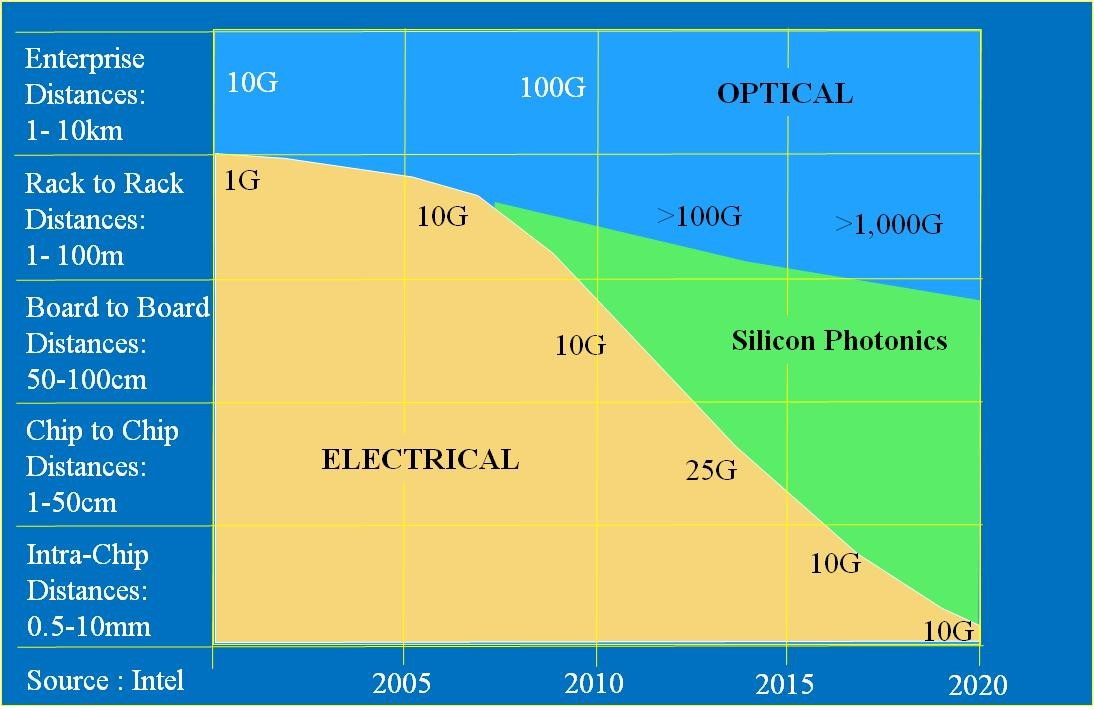
\includegraphics[width=\textwidth]{./Pictures/figure1.jpg}
	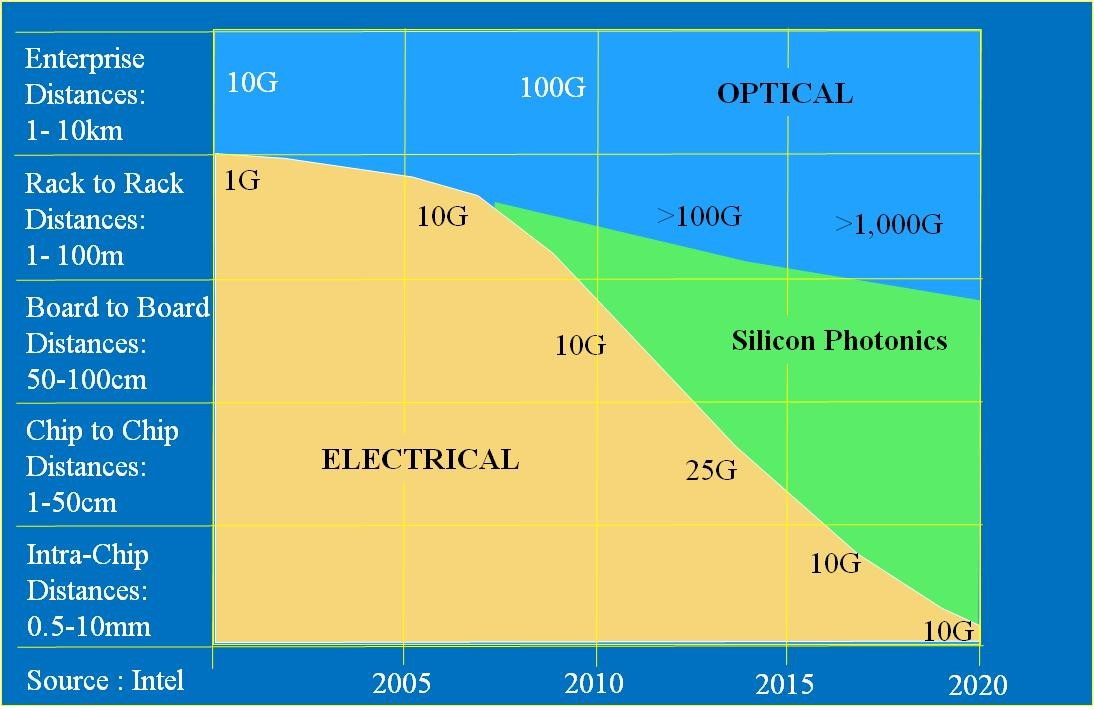
\includegraphics[width=12cm]{./Pictures/figure1.jpg}
	\caption{在不同通信距离下,电互联、硅基光通信和光纤通信的速率使用范围 \cite{Zuffada2012}}
	\label{figure1}
\end{figure}

硅基平台(Silicon-On-Insulator),即由硅衬底、二氧化硅绝缘层和硅薄膜构成的平台,不仅在传统半导体电子领域中有广泛运用,在微纳光子系统中也被广泛采用。硅基平台也成为了实现光电子集成芯片的理想平台。虽然,过去基于III-V材料的InP平台光电子平台已经实现了复杂的通信系统\cite{Meint2014an},比如片上波分复用的光收发器和多波长路由器,但是大规模应用需要价格低廉。除此之外,InP平台上的波导,垂直方向折射率差小只有1\%,导致波导的宽度和高度尺寸在工作波长量级。而硅基光波导在水平和高度方向都有将近60\%的高折射率差,因此光波导尺寸小。又因为硅基平台晶片的单位面积成本比InP晶片低,尺寸又比InP晶片大,所以硅基平台单个光器件的成本远小于InP平台。此外,硅基平台的小尺寸波导传输损耗最低达到 0.4 dB/cm \cite{Tsuyoshi2016low} 小于InP波导的最低传输损耗约为 1 dB/cm \cite{Meint2014an}。从而,硅基光电子平台越来在光通信领域受到人们的关注。

硅基光通信模块作为硅基光电子集成芯片的一个重要应用方向,其具有带宽大,功耗低,成本低的特点。图 \ref{figure1} 描述了电互联、硅基光通信和传统光纤通信和在不同距离下的适用速率范围 \cite{Zuffada2012}。图 \ref{figure1} 也预测了随着通信速率的逐年提高,硅基光通信在短距离将逐渐代替电互联。因此,硅基光集成芯片越来越受到各国的关注。美国在2004年率先提出了EPIC (Electronic and Photonic Integrated Circuits on Si)计划,研究硅基光电子集成平台,这将有助于通信,传感,微波光子学等研究方向的发展\cite{Shah2005}。欧洲在2008年提出了HELIOS (pHotonics ELectronics functional Integration on CMOS)计划,研究基于CMOS工艺的硅基光电子平台 \cite{HELIOS}。日本也紧跟而上,在2010年提出了PECST(Photonics and Electronics Convergence System Technology),推动硅基光电子平台的发展,实现芯片间的通信带宽密度达到10 Tb/s/cm\SP{2}\cite{Arakawa2013Silicon}。

光集成芯片的概念最早是由美国贝尔实验室的Miller在1969年提出来的\cite{miller1969}。随后1993, 美国空军科学研究实验室的Richard A. Soref提出了的硅基光电子集成芯片的概念\cite{Soref1993},见图 \ref{figure2} (a). 硅基光电子芯片是在同一片硅衬底上集成了负责逻辑和驱动的晶体管,负责光通信的激光器,调制器,光放大器,光探测器,光无源结构,光波导和光纤的耦合结构。在接下来的20多年内,全世界的知名高校和半导体公司都投入大量资金到这个领域中。在2011年,见图 \ref{figure2} (b), Intel厚积薄发推出了世界上第一款硅基光通信芯片包含了片上的激光器,纯硅调制器和硅锗探测器的光通信模块,实现了单通道12.5 Gbps的传输速率 \cite{Paniccia2011}。在2012年,见图 \ref{figure2} (c, d), IBM紧接发布了利用改进的90 nm CMOS工艺线,实现了在单个硅片上同时集成晶体管和的25 Gbps的光调制器和探测器 \cite{Assefa2012}。Intel虽然集成了激光器但是没能在单片上同时集成晶体管,而IBM虽然集成了晶体管,却没能集成激光器并且缺少完整光收发链路的展示。在2015年,美国伯克利大学和麻省理工大学的Chen Sun等首次展示了直接在商业化的45 nm CMOS流水线上,制作硅基光电子集成芯片 \cite{sun2015single}。该单块芯片,见图\ref{figure3} (a), 上不仅包含处理器,内存,还包含光收发模块。并且他们还展示了如图 \ref{figure3} (b) 所示的处理器的芯片和内存的芯片直接用光互联技术进行时时数据的运算和处理。虽然该硅基光电子芯片依旧缺少片上的激光器和放大器,但是该芯片是目前最复杂的单片硅基光电子芯片,包含了700万个晶体管和850个光模块。

\begin{figure}[htb]
	\centering
	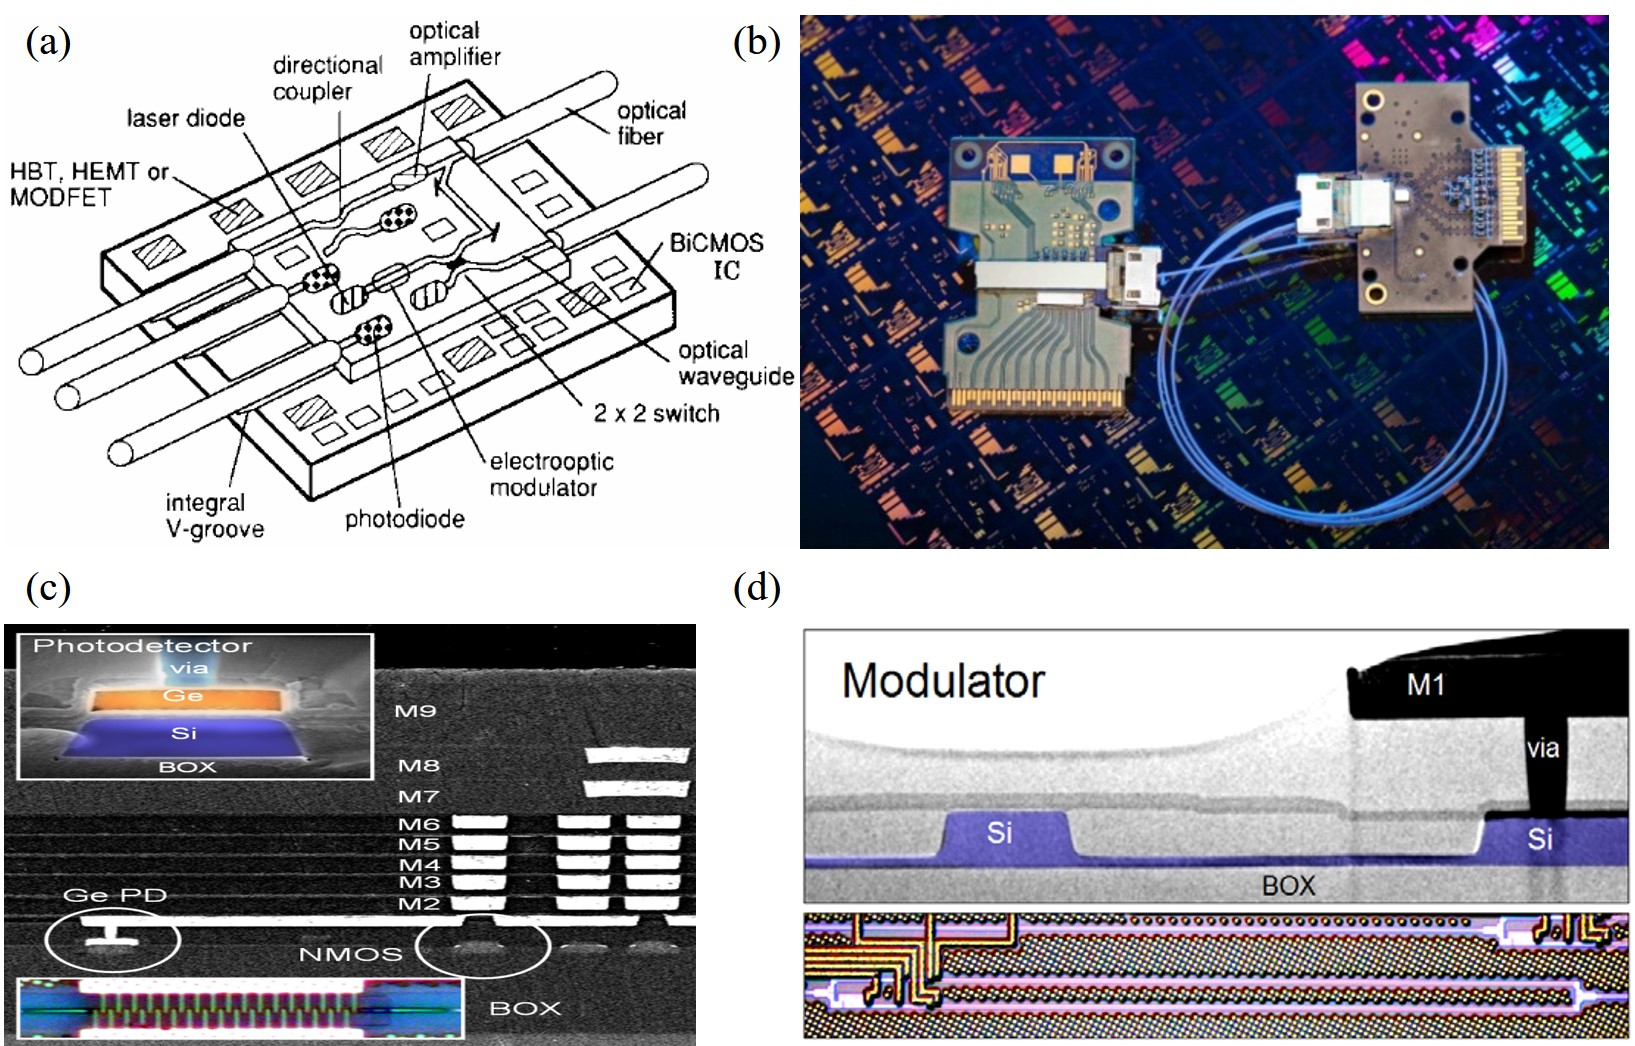
\includegraphics[width=12cm]{./Pictures/figure2.jpg}
	\caption{ (a) 最早的硅基光电子芯片概念图 \cite{Soref1993};(b)Intel的硅基光收发模块\cite{Paniccia2011};(c,d) IBM的硅基探测器和调制器\cite{Assefa2012}}
	\label{figure2}
\end{figure}

\begin{figure}[htb]
	\centering
	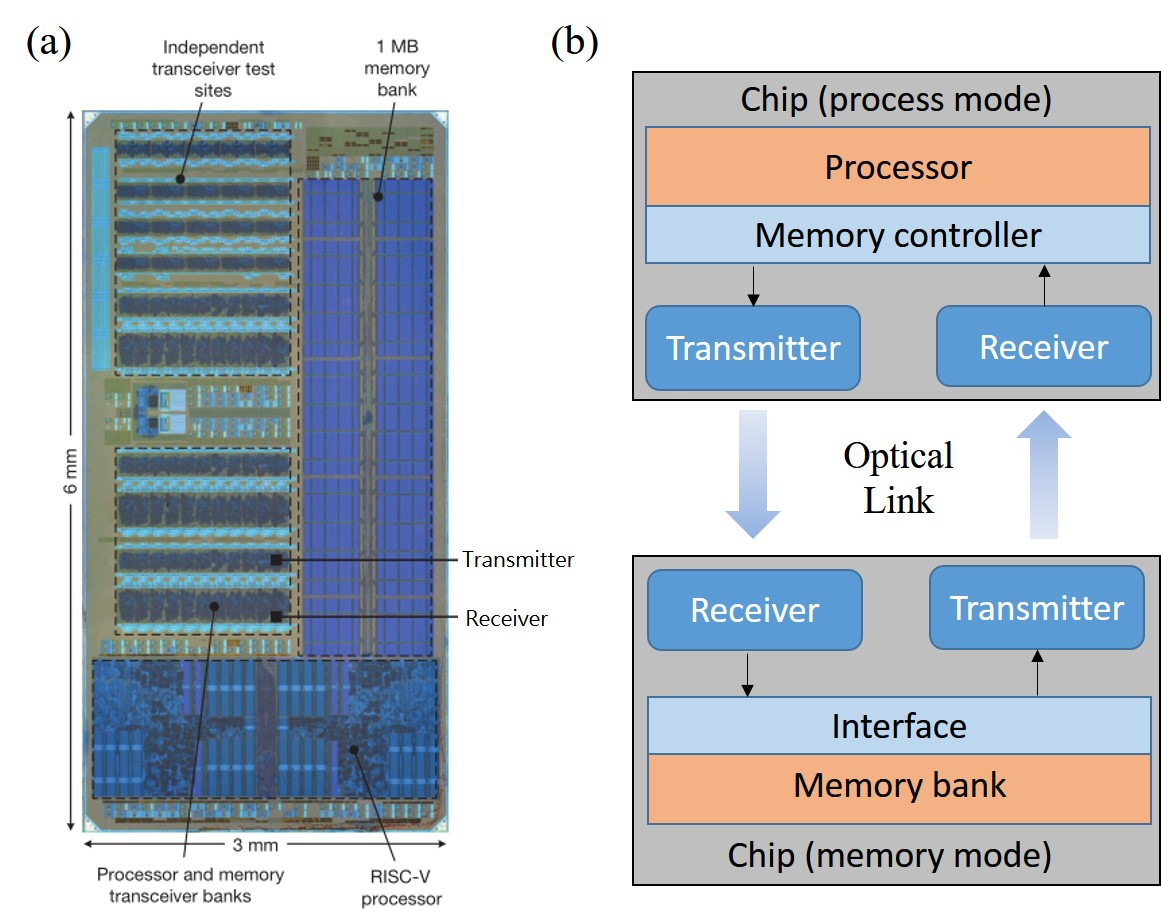
\includegraphics[width=10cm]{./Pictures/figure3.jpg}
	\caption{ (a) 单片硅基光电子芯片,包含处理器,内存,光收发模块\cite{sun2015single};(b) 处理器芯片和内存芯片间光互联示意图}
	\label{figure3}
\end{figure}

\section{硅基光调制器}
硅基光调制器做为硅基光通信模块中不可缺少的一环,用于电信号向光信号的转化,影响着光通信模块的通信速度和能耗,一直硅基光通信领域的重点和难点。虽然硅基光调制器的光学结构,电极和材料可以有很多种,但是评价硅基光调制器的性能好坏可以由以下5个指标看出:
\begin{enumerate}[(1)]
	\item 调制速率(Data Transfer Rate, BR),通常用单位时间内多少比特的信息从电信号转化为光信号来表示,单位是bps。在光调制器中调制速率一般是Gbps的数量级。描述调制器的速率还可以通过调制带宽的3 dB来表述($f$\SB{3-dB})。数字信号光调制器的电光响应频谱如同一个低通滤波器,$f$\SB{3-dB}就是调制器的电光响应降低到最大值的一半时的频率。调制器的调制速率大于调制器的调制带宽,两者的关系可以通过香农有噪信道编码定理(Shannon–Hartley theorem)联系。当没有噪声时,对于二进制编码调制速率可以达到调制带宽的两倍。
	\item 消光比(Extinction Ratio, ER)也称作调制深度,表示光在信号0和1时强度的比值,用dB表示。 消光比越高,信噪比也越好。
	\item 能耗(Energy Consumption, EC)表示将单个比特的信息从电信号转化到光信号上所消耗的电的能量。能耗的公式如下所示:
		\begin{equation}
		\label{Equ:EC}
		EC = CV_{pp}^{2}/4 + I_{average}V_{bias}/BR
		\end{equation}
	该公式分为两部分,第一部分是动态调制的能耗和第二部分是静态偏置的能耗。其中$C$是调制区域的等效电容,$V_{pp}$是驱动电压的峰峰值,$I_{average}$是直流偏置和吸收光子的而产生电流,$V_{bias}$是偏置电压,BR是调制速率。
	\item 插入损耗(Insertion Loss,IL)是调制器在全通状态下的输入光信号和输出信号的差值。插入损耗也会影响产生信号的信噪比。这些损耗包含调制器引入的反射,材料的损耗,模式不匹配引起的损耗。
	\item 器件尺寸(Footprint)是硅基光调制器光学结构加上调制区域电极结构的总尺寸。调制器的尺寸也是在硅基光调制器比较重要的参数,影响了调制器的集成度。尺寸越小的硅基光调制器在硅基光通信模块中越受到欢迎。
	\item 光学带宽(Optical bandwidth)是硅基光调制器调制波长的范围。通常谐振型的光调制器,调制波长窄,只能在谐振波长处调制。而其他类型的光调制器有比较大的光学带宽。	
\end{enumerate}

下面将讨论目前硅基光调制器在光学结构和电学结构的研究成果,概括不同材料在硅基平台上实现光调制器的最新进展。
\subsection{硅基光调制器的光学结构}
硅基光调制器如同传统的光调制器,是利用电信号改变材料折射率的实部或者虚部,从而调制器光信号的相位或者幅度。材料的折射率可以用可以表示为:
\begin{equation}
	\label{Equ:index}
	\widetilde{n(\lambda)} = n(\lambda) + j\kappa(\lambda) =  n(\lambda) + j\frac{\lambda\alpha(\lambda)}{2\pi}
\end{equation}
其中$n$为材料折射率的实部,$\kappa$为材料折射率的虚部(称作消光系数)。$\alpha$是材料单位长度的损耗。$n, \kappa, \alpha$都是和波长相关。其中$\kappa$和$\alpha$是线性关系。$n$和$\kappa$可以用通过Kramers-Kronig联系到一起\cite{o1981kramers}。

\begin{figure}[htb]
	\centering
	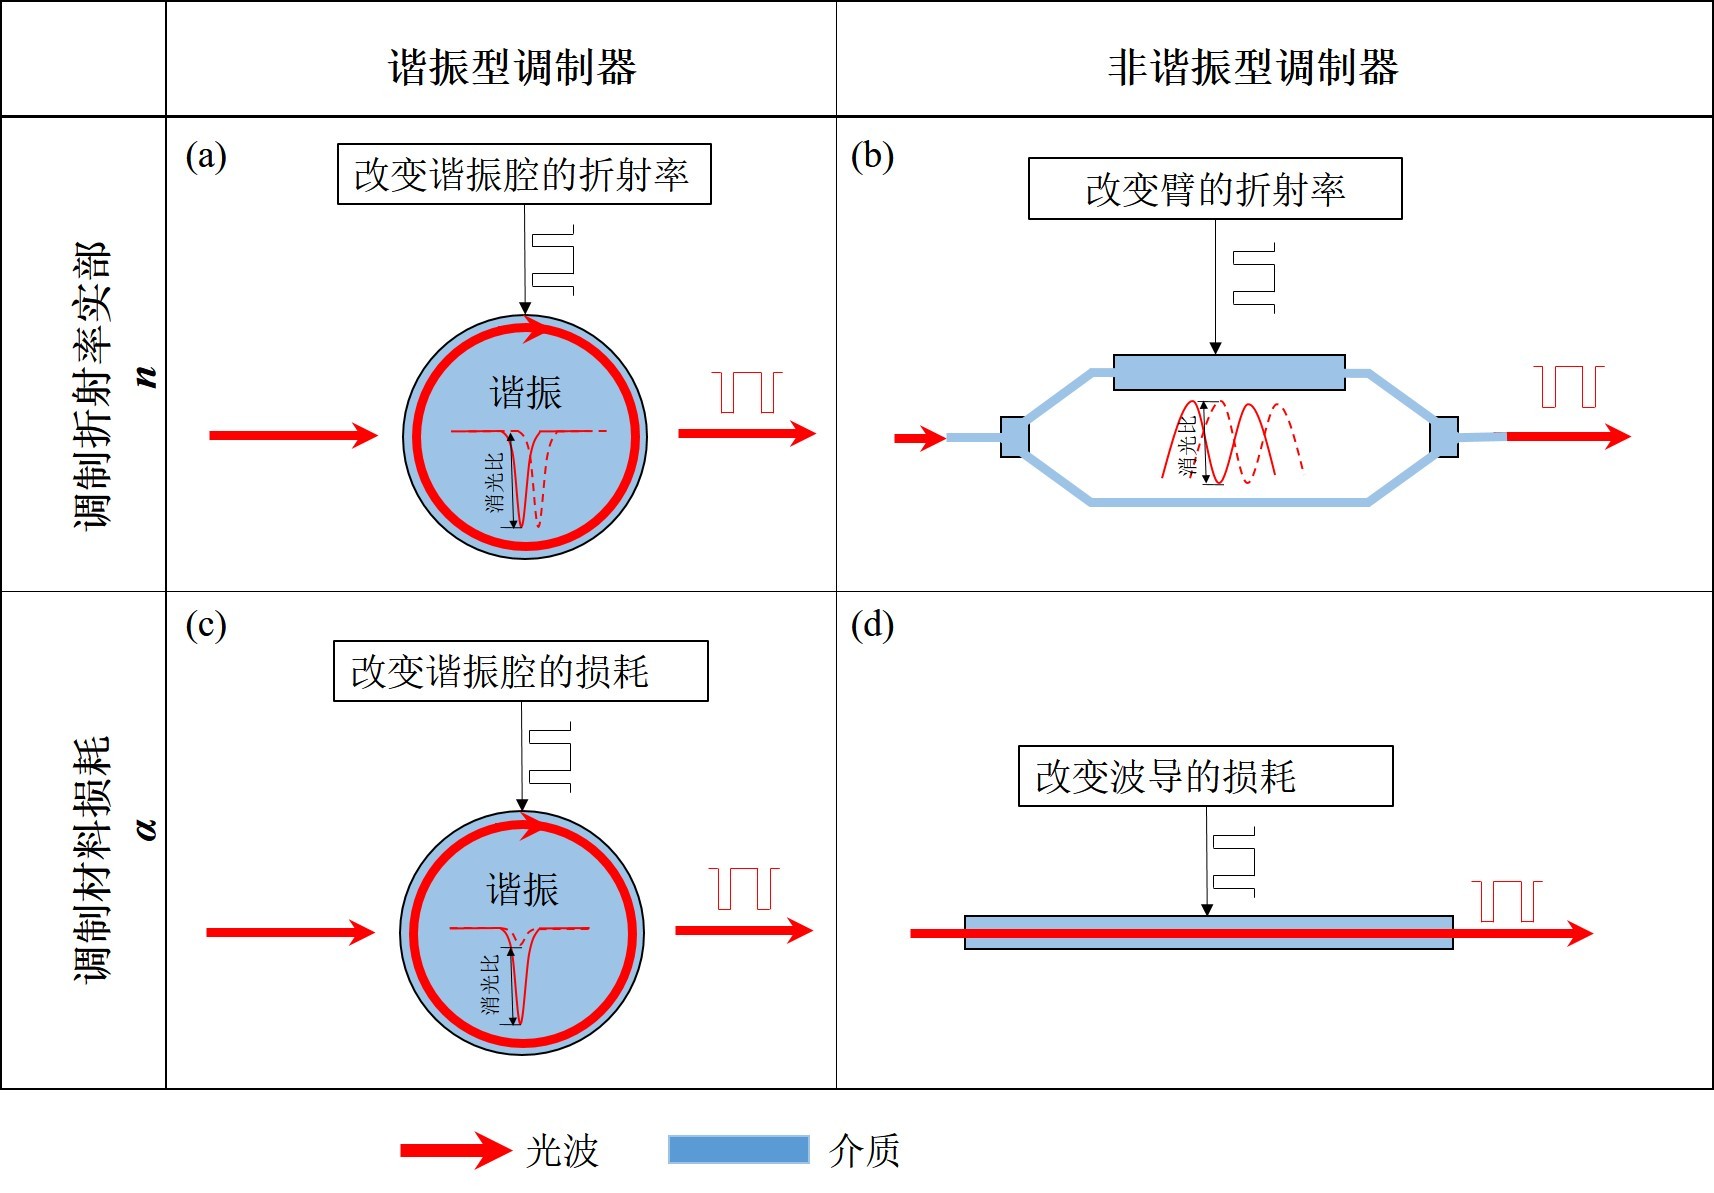
\includegraphics[width=12cm]{./Pictures/fig_mod_opt_type.jpg}
	\caption{ (a, b) 分别是通过调制折射率实部的谐振和非谐振型光调制器;(c, d)分别是通过调制材料损耗的谐振和非谐振型光调制}
	\label{fig_mod_opt_type}
\end{figure}
图 \ref{fig_mod_opt_type} 概括了硅基光调制器的光学结构的四大类型。前两类都是利用电光效应改变光的相位,再利用光学结构转化为光强度的变化。后两类是利用电吸收效应直接改变光的强度。

第一类如图\ref{fig_mod_opt_type} (a) 所示,通过调制折射率实部,改变谐振波长的位置,实现特定波长的调制。这类调制器的特点是结构紧凑,速度快,驱动电压小,能耗低。图\ref{fig_mod_opt_type_real} (a) 展示了最早利用这种结构实现的小尺寸硅基光调制器的实例\cite{xu2005micrometre}。该调制器利用载流子注入效应,调制硅波导的折射率,移动微环的谐振峰,从而实现谐振波长处光强的调制。

第二类如图\ref{fig_mod_opt_type} (b) 所示,也是通过调制折射率实部,实现相位的调制。这类调制器但是利用马赫曾德(MZI)结构,将一根波导上的相位变化,转变成强度调制器。其特点是速度快,光学带宽大。图\ref{fig_mod_opt_type_real} (b) 展示了最早利用这种结构的实现速度达到Gbps的硅基光调制器实例\cite{liu2004high}。该调制器也是利用载流子注入效应,实现马赫曾德一臂的相位变化,从而调制输出的光强。

第三类如图\ref{fig_mod_opt_type} (c)所示,通过调制微环的损耗,从而影响微环的谐振波长处的临界耦合系数,从而调制谐振波长的强度。这类调制器的特点是结构紧凑,驱动电压低,能耗低,速度快。图\ref{fig_mod_opt_type_real} (c) 展示了最早利用这种结构的硅基光调制器的实施方案\cite{Midrio2012graphene}。该调制器利用微环中部分硅波导上的石墨烯,调制石墨烯的损耗,导致微环损耗的变化,从而调制谐振波长处光的强度。由于这类调制器是最近2012年才提出的,目前只在氮化硅平台上有实例\cite{phare2015graphene},在硅基平台上没有实例,只有理论分析的结果\cite{Midrio2012graphene}。

第四类如图\ref{fig_mod_opt_type} (d)所示,直接通过改变波导的损耗,实现光强度的调制。这类调制器的特点是结构紧凑,能耗低,速度快,光学带宽大。图\ref{fig_mod_opt_type_real} (d) 展示了利用这种结构的硅基光调制器实例\cite{tang201150}。该调制器是将InP混合集成到硅波导上,再利用InP多量子阱材料(Multiple Quantum Well, MQW)中量子束缚Stark效应(Quantum Confined Stark Effect, QCSE)实现在不同电压下,材料吸收峰的移动,导致波导的损耗的变化,从而实现光强度的变化。

这四类调制器中的马赫曾德结构除了能用于将光的相位变化转变成强度变化外,还经常被用于高级调制码型的发生器,比如文献[\citenum{Dong2012coherent}]中就利用马赫曾德结构实现正交相移键控(Quadrature Phase-Shift Keying, QPSK)调制码形,并且结合了偏振复用,使单通道的调制速度提高到112 Gbps。
\begin{figure}[htb]
	\centering
	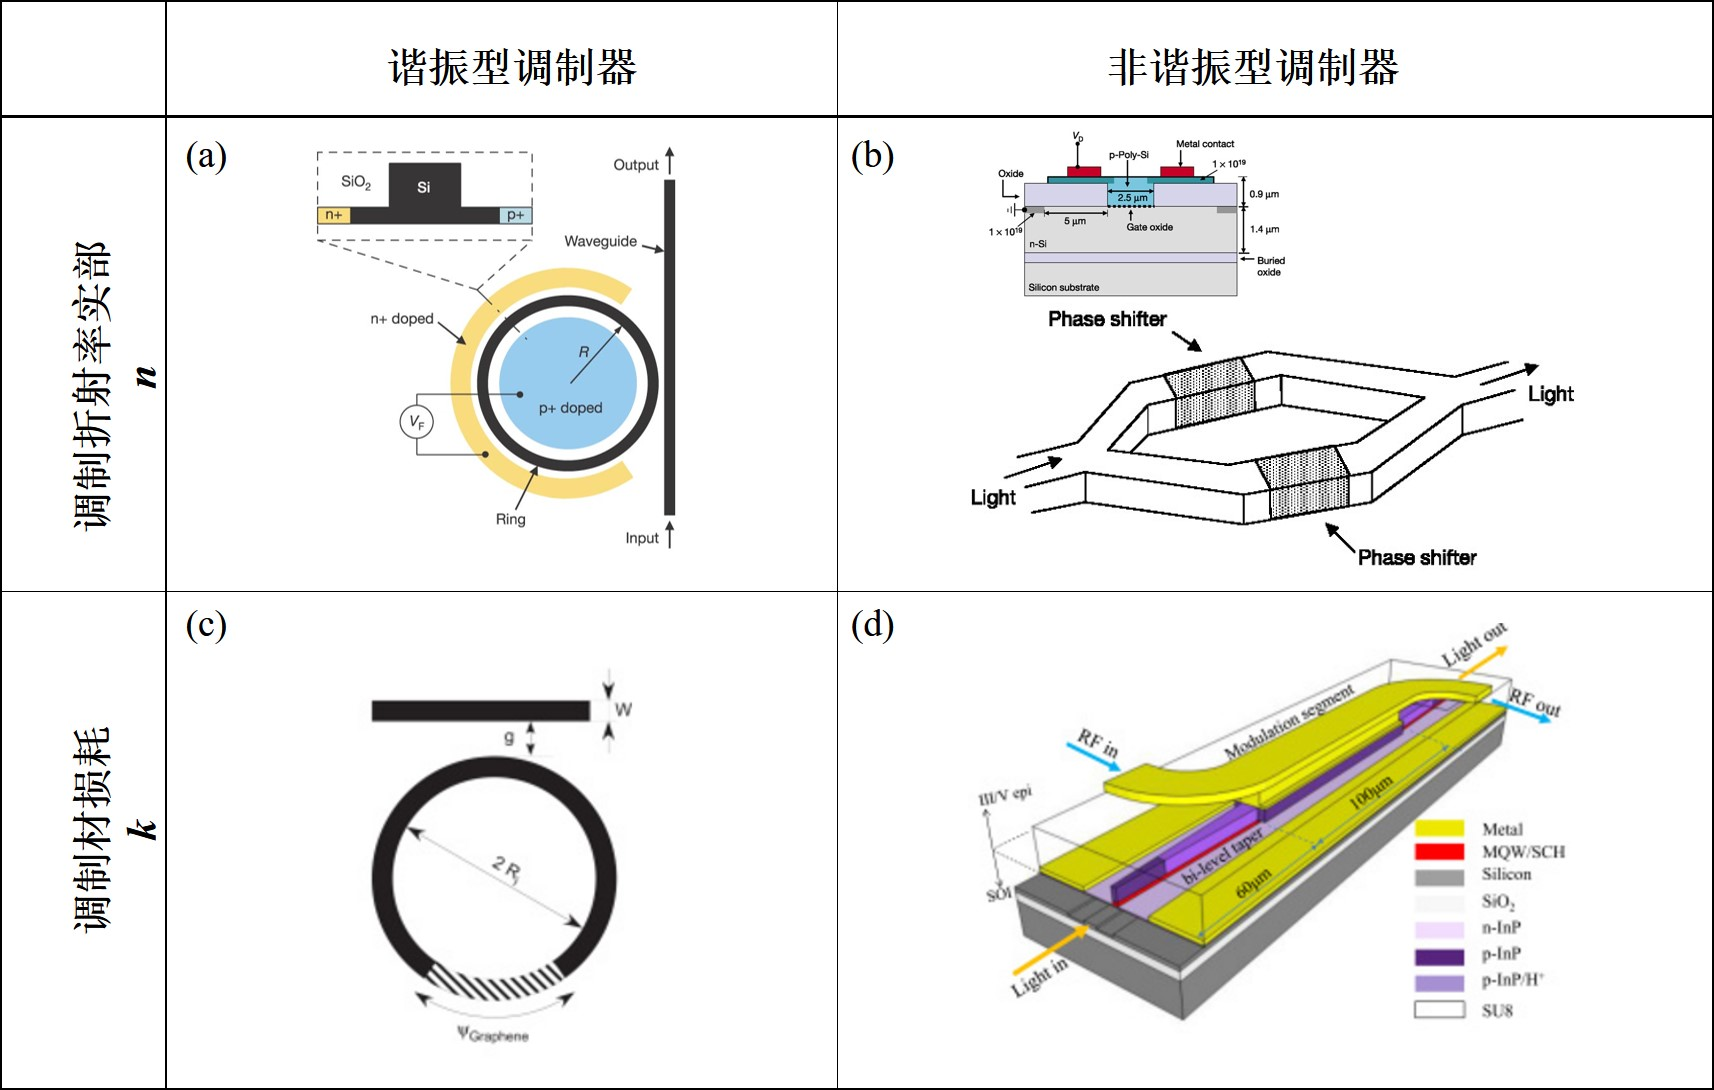
\includegraphics[width=12cm]{./Pictures/fig_mod_opt_type_real.jpg}
	\caption{ (a, b) 分别是通过调制折射率实部的谐振和非谐振型光调制器的实例\cite{xu2005micrometre,liu2004high};(c, d)分别是通过调制材料损耗的谐振和非谐振型光调制的实例\cite{Midrio2012graphene,tang201150}}
	\label{fig_mod_opt_type_real}
\end{figure}

\subsection{硅基光调制器的电极结构} \label{electrostructure}
硅基光调制器的电极结构对调制速率和能耗也有很大影响。图\ref{fig_mod_ele_type}展示了目前硅基光调制器所有的四种电极结构。这四种电极结构已经在InP光调制器和LiNbO\SB{3}光调制器上被广泛应用。下面将讨论这四种电极结构特点。

\begin{figure}[htb]
	\centering
	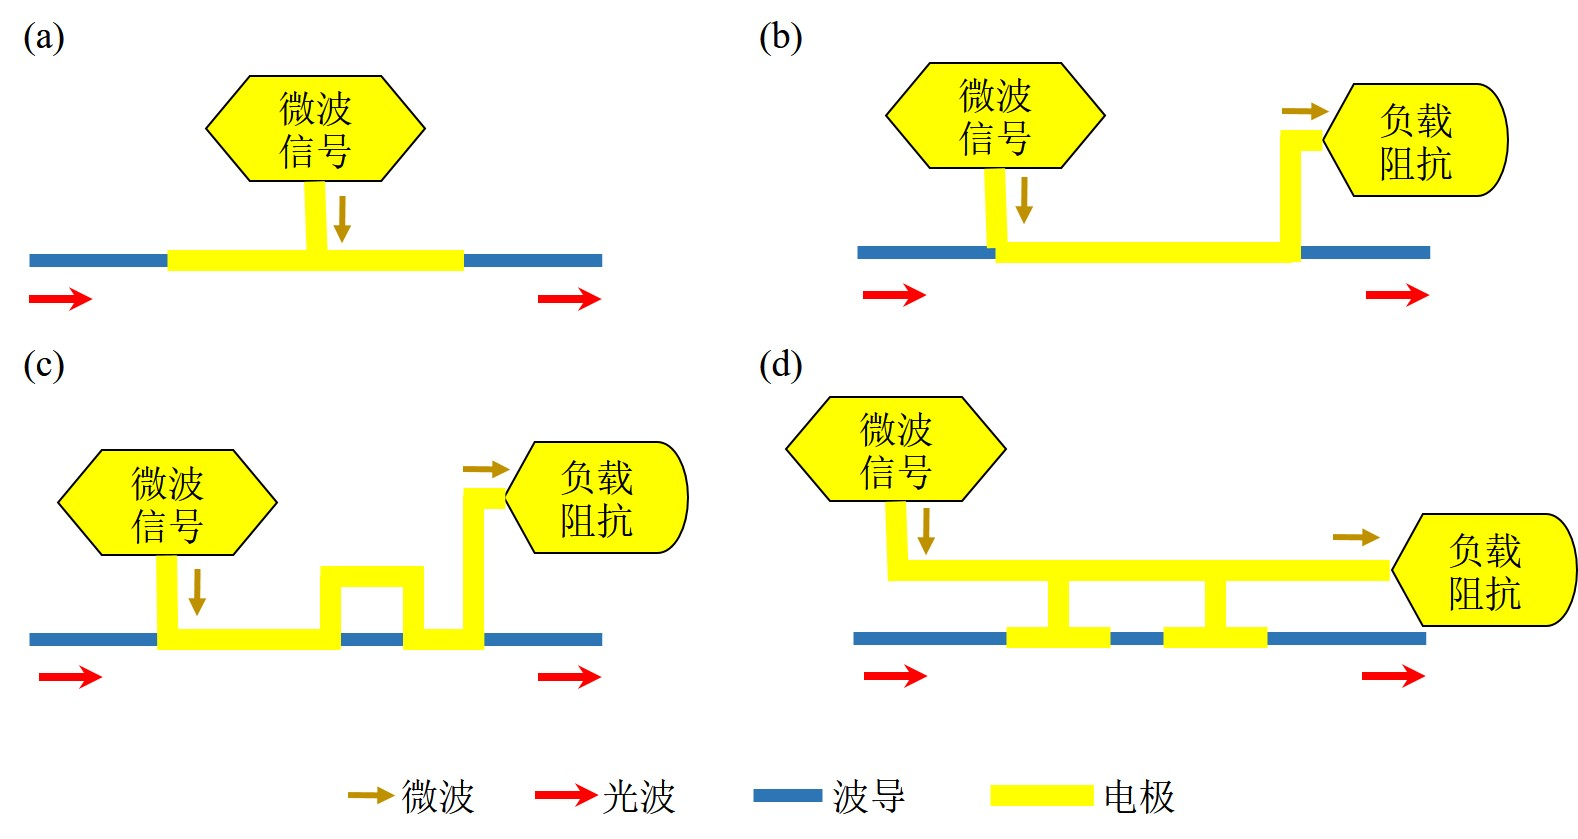
\includegraphics[width=12cm]{./Pictures/fig_mod_ele_type.jpg}
	\caption{ (a) 集总电极;(b)行波电极;(c)分段传输线电极;(d)电容负载行波电极}
	\label{fig_mod_ele_type}
\end{figure}

第一种电极称为集总电极(Lumped Electrode, LE)如图\ref{fig_mod_ele_type} (a)所示, 这种电极在调制区域的长度小于100 $\mu m$的硅基光调制器中被广泛使用,尤其是小型的谐振型硅基光调制器。由于这类电极末端没有负载是开路,导致微波信号末端反射,集总电极上成为驻波,从而降低所需外界的调制电压,同时也避免了偏置电压在负载上损失的能耗。因此,集总电极在小尺寸,低驱动电压,低能耗的电极上有广泛的应用。图\ref{fig_mod_ele_type_real} (a)展示了集总电极用于InP混合集成到硅波导上的调制器\cite{tang2012energy},实现了低能耗,低驱动电压,小尺寸的调制器。

第二中电极称为行波电极(Traveling Wave Electrode, TWE)如图\ref{fig_mod_ele_type} (b)所示,这种电极在调制区域大于100 $\mu m$的硅基调制器中被广泛使用,尤其是马赫曾德的硅基光调制器。由于这行波电极调制器需要将电极考虑成为传输线,因此需要设计电极本征阻抗与标准的微波器件的本征阻抗50 $\Omega$相匹配,并且使传输线的传播常数和波导中光的传播常数相匹配,从而尽可能提高调制器的调制带宽。因此,使用行波电极的调制器调制速度高于集总电极的调制器,但是在尺寸,驱动电压,能耗上差于集总电极的调制器。图\ref{fig_mod_ele_type_real} (b)展示了行波电极用于InP混合集成到硅波导上的调制器\cite{tang2012energy},实现了高速的硅基光调制器。

第三种电极称为分段传输线电极(Segmented Transmission Line Electrode, STLE)如图\ref{fig_mod_ele_type} (c)所示, 这种电极也是主要用于调制长度大于100 $\mu m$以上,并且电极的本征电阻和50 $\Omega$相差大,或者微波和光波的传播常数相差较大的硅基光调制器。分段传输线电极是行波电极的一个更为普遍的形式,相比行波电极,其调制带宽可以进一步提高,但是能耗不会有所减少,而尺寸将更进一步增大,。图\ref{fig_mod_ele_type_real} (c)展示了分段传输线电极用于InP混合集成到硅波导上的调制器\cite{tang2012energy},实现了目前调制速度最快的硅基光调制器。

第四种电极称为电容负载行波电极(Capacitively-Loaded Traveling-Wave Electrode, CLTWE)如图\ref{fig_mod_ele_type} (d)所示, 这种电极在硅基光调制器中的应用比较少,主要用于调制长度大于500 $\mu m$以上,并且电极的本征电阻和50 $\Omega$相差大,或者微波和光波的传播常数相差较大的硅基光调制器。由于电容负载行波电极整体和如同行波电极一样,但在单个周期内,调制器区域是集总电极,因此这类电极用于兼顾传输速度和低驱动电压。不过,由于在单个调制器区域还有没参与调制的电极,因此电容负载行波电极的尺寸比较大。图\ref{fig_mod_ele_type_real} (d)展示了电容负载行波电极用于InP混合集成到硅波导上的调制器\cite{tang2012energy},实现了马赫曾德的光调制器。

这四种电极各有优缺点,如果需要尺寸小,能耗低的调制器,可以采用集总电极。如果需要尽可能高的调制速度,或者调制器区域长度比较长时则可以采用行波电极或分段传输线电极结构。而电容负载行波电极是集总电极和分段传输线折中的形式,可以在这两种电极都无法满足要求的情况下使用。
\begin{figure}[htb]
	\centering
	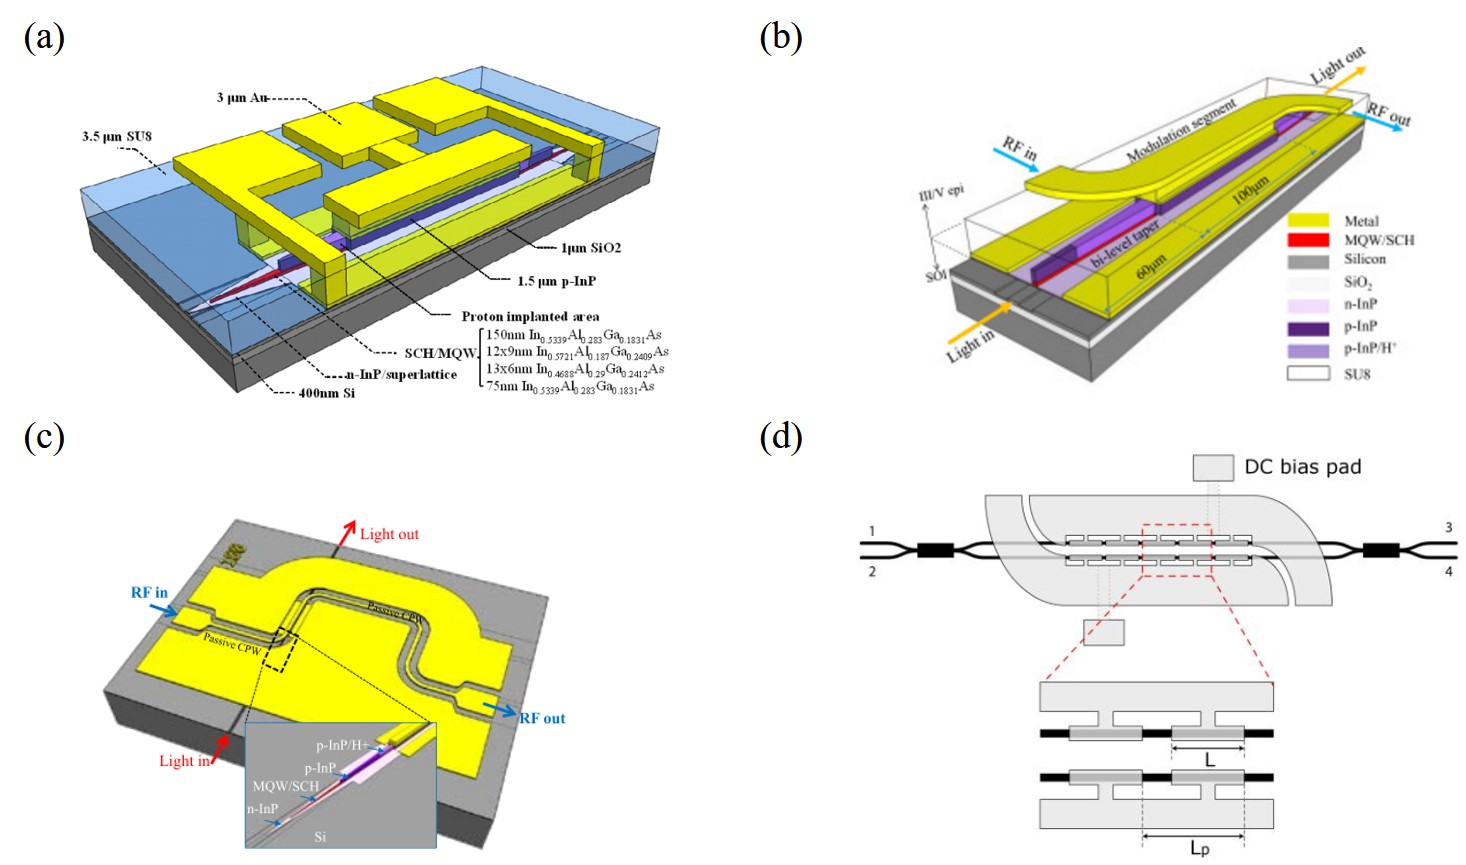
\includegraphics[width=12cm]{./Pictures/fig_mod_ele_type_real.jpg}
	\caption{ (a) 集总电极的实例\cite{tang2012energy};(b)行波电极实例\cite{tang201150};(c)分段传输线电极实例\cite{tang2012over};(d)电容负载行波电极实例\cite{chen2011forty}}
	\label{fig_mod_ele_type_real}
\end{figure}
\subsection{纯硅基光调制器} \label{pure_simodulator}
纯硅的光调制器可以与标准的半导体工艺完美结合,满足实际调制器小尺寸,低功耗或者高速,大光学带宽的需求,而且调制器的加工成本低。因此,纯硅硅光调制器一直是硅基光调制器中最热门的研究方向。不过由于硅是反演中心对称的晶体,导致它不具有线性电光效应,即Pockels效应,并且在通信1.3 $\mu m$ 和 1.55 $\mu m$处,二阶非线性Kerr也很弱\cite{soref1987electrooptical}。虽然硅的热光系数很大,但是热光效应作为光调制器速度太慢\cite{cocorullo1992thermo}。

目前,纯硅基光调制器采用的是等离子色散效应(plasma dispersion effect)实现速度达到Gbps以上的光调制器。硅基光调制器采用三种方式实现等离子色散效应,分别是载流子注入(Carrier injection),载流子聚集(Carrier accumulation)和载流子耗尽(Carrier depletion)。

载流子注入的实现方式是最早被提出来的,但是靠这种方式的调制器速度由硅中少数载流子寿命决定。目前载流子注入的光调制器速度最多达到Gbps,通过预加重(pre-emphasis)的特殊码形速度目前最高达到18 Gbps\cite{manipatruni2007high}。

载流子聚集对的方式是最早实现高于1 Gpbs的纯硅基光调制器。载流子聚集调制器是通过将自由载流子聚集到波导中的薄介质层附近从而实现改变折射率。因此,载流子聚集的调制器速度突破了少数载流子寿命的约束,调制速度由等效电容和电阻决定速率。由于薄介质层的厚度薄,载流子聚集效率低,等效电容大,从而影响了最高的速度,目前载流子聚集的光调制器最快达到25 Gbps\cite{fujikata201025}。

载流子耗尽的方式是目前实现最快硅基光调制器。载流子耗尽调制器是通过外界反向偏压,控制波导中耗尽区和光场相互作用的面积从而实现调制。因此,载流子耗尽的调制器也突破了载流子寿命的约束,调制速度也由等效电容和电阻决定速率。由于耗尽区的宽度可以通过本pn结的掺杂浓度,或者pin结构中i层的厚度,或者反向偏压的大小控制,因此等效电容可以方便的根据实际所需速率设计。目前载流子耗尽的光调制器最快速度达到了60 Gbps\cite{Xiao201360}。

由于纯硅基调制器和半导体工艺完美结合,因此大学实验室只能提供设计,然后提交给拥有完全流水线的半导体代工公司(比如比利时的Imec-ePIXfab \cite{Imec, absil2015silicon}、新加坡的OpSIS-IME \cite{novack201330}、美国的IBM的45nm的SOI半导体流水线\cite{narasimha2006high}等)生产制作。另外,中国的中芯国际(Semiconductor Manufacturing International Corporation, SMIC)也提供硅调制器的加工\cite{xu2012high,xiao2013high,Xiao201360}。表\ref{sil_mod}总结了近期纯硅基光调制器方面的最好的结果。目前纯硅基光调制器的最高调制速度达到了60 Gbps,能耗最低能到0.1 fJ/bit,驱动电压最低需要50 mV。

{
	\begin{table}[htb]
		\zihao{5}
		\caption{比较近期纯硅基光调制器的性能。PhC: 光子晶体;Ring:微环; Zigzag:锯齿;Disk:微盘;MZI:马赫曾德}
		\label{sil_mod}
		\centering
		\begin{tabular}[t]{p{1.5cm}ccp{1.2cm}ccccccc}
			\hline
			掺杂方式 & 光学结构 & 电极结构 & 调制区尺寸 & 调制速度 & 动态能耗 & 消光比 & 插入损耗 & 调制电压\\
			\hline
			lateral pn \cite{xiao2013high,Xiao201360} & MZI & TW  & 750 $\mu m$ & 60 Gbps & - & 4.4 dB & 2.0 dB& 6.5 V\\
			zigzag pn\cite{Xiao201360} & Ring & LE & 22 $\mu m$ & 60 Gbps & - & 4.2 dB & - & 6 V\\
			vertical pn\cite{timurdogan2014ultralow} & Disk & LE & 4.8 $\mu m$ & 44 Gbps & 17.4 fJ/bit & 8.0 dB & 0.92 dB & 2.2 V\\
			lateral pin\cite{shakoor2014ultra} & PhC & LE & ~6.0 $\mu m$ & 1 Gbps & 0.1 fJ/bit & 2.0 dB & - & 50 mV\\			
			lateral pn\cite{Pantouvaki201556} & Ring & LE & 10 $\mu m$ & 56 Gbps & 45 fJ/bit & 4.0 dB & 3.0 dB& 2.5 V\\
			lateral pipin\cite{Ziebell201240} & MZI & TW & 950 $\mu m$ & 40 Gbps & - & 3.2 dB & 2.5 dB & 6 V \\
			lateral pin\cite{Baba201350} & Ring & LE & 20 $\mu m$ & 50 Gbps & - & 4.6 dB & 5.2 dB & 1.96 V\\
			lateral pn\cite{Ding2013electro} & MZI & TW & 2 $mm$ & 40 Gbps & 32.4 fJ/bit & 3.5 dB & 12.5 dB & 0.36 V\\
			\hline
		\end{tabular}
	\end{table}
}

纯硅基光调制器波导的掺杂方式根据不同等离子色散实现方式分有很多种\cite{reed2010silicon},在此主要介绍三种常用且特色的方案,如图\ref{fig_silicon_mod_cross}所示。表\ref{sil_mod}也展示不同掺杂方式的硅基光调制器最新最好的性能。
第一种是水平掺杂的pn结或者pin结,如图\ref{fig_silicon_mod_cross}(a)所示。这种掺杂方式使用最为广泛,用于目前调制速度达到60 Gbps的纯硅基MZI光调制器(如图\ref{fig_silicon_mod}(a)所示)\cite{xiao2013high}。另外,驱动电压只有50 mV 并且能耗只有0.1 fJ/bit的光子晶体(Photonic Crystal, PhC)结构的纯硅基光调制器(如图\ref{fig_silicon_mod}(b)所示)也是采用了水平掺杂的pn结\cite{,shakoor2014ultra}。
第二种是交趾掺杂和其改进型的锯齿掺杂,如图\ref{fig_silicon_mod_cross}(b)所示。这种掺杂方式目前主要用于提高单位长度的调制效率,目前调制速度最快达到60 Gbps的纯硅基微环光调制器(如图\ref{fig_silicon_mod}(c)所示)就是采用这种结构\cite{Xiao201360}。
第三种是在2014年才提出的垂直方向pn结,如图\ref{fig_silicon_mod_cross}(c)所示。通过种掺杂方式,并且结合微盘结构(如图\ref{fig_silicon_mod_cross}(c)所示),具有pn掺杂谐振型光调制器中最高的电光效应,达到了250 pm/V,这是之前的十倍\cite{timurdogan2014ultralow}。

\begin{figure}[htb]
	\centering
	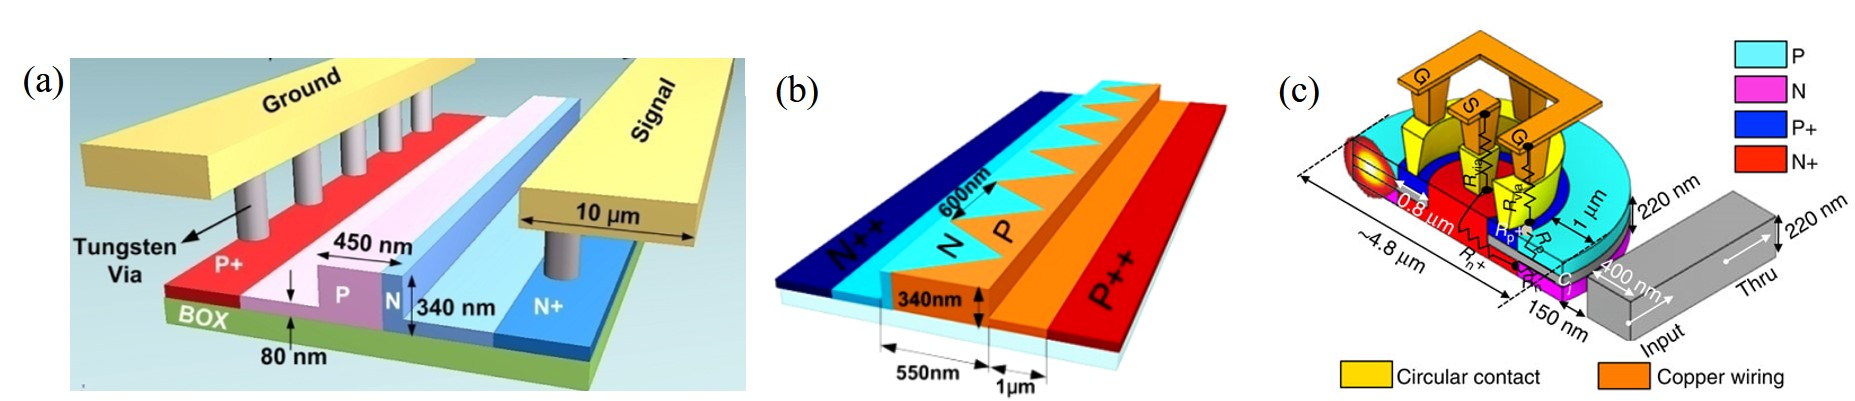
\includegraphics[width=15cm]{./Pictures/fig_silicon_mod_cross.jpg}
	\caption{ (a) 中心偏移的水平pn结\cite{xiao2013high};(b)齿状交趾的纵向pn结\cite{Xiao201360};(c)垂直方向的pn结\cite{timurdogan2014ultralow}}
	\label{fig_silicon_mod_cross}
\end{figure}

\begin{figure}[htb]
	\centering
	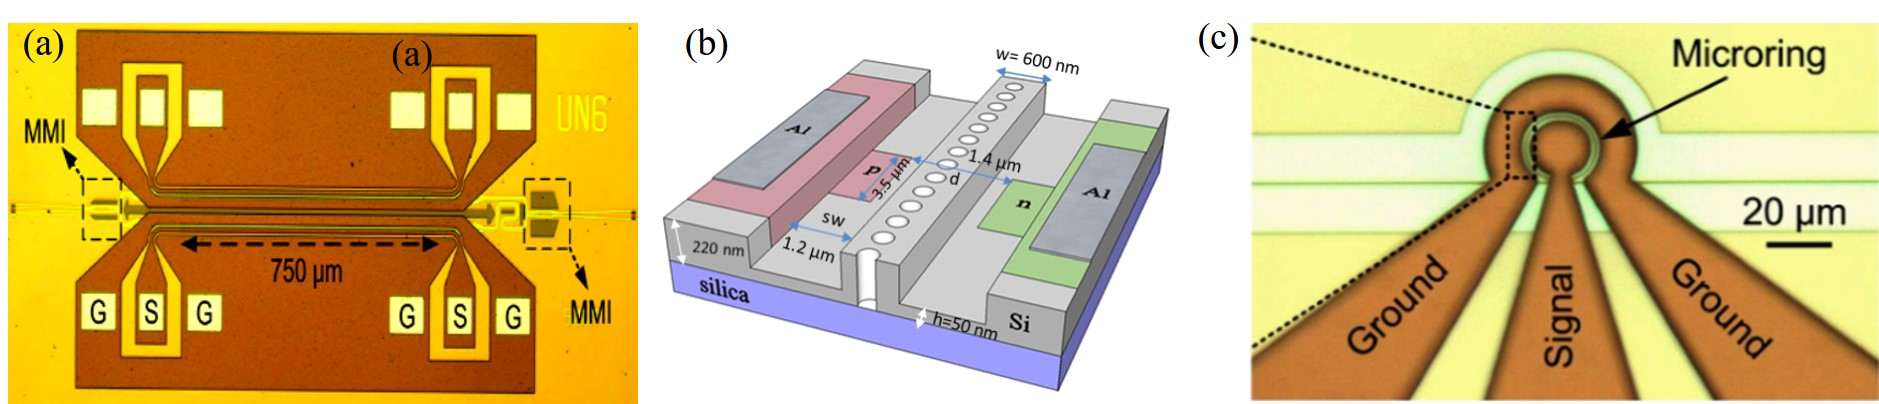
\includegraphics[width=15cm]{./Pictures/fig_silicon_mod.jpg}
	\caption{ (a) 60 Gbps的MZI纯硅基光调制器\cite{Xiao201360};(b)能耗0.1 fJ/bit的光子晶体纯硅基光调制器\cite{shakoor2014ultra};(c) 60 Gbps的锯齿掺杂微环纯硅基光调制器\cite{Xiao201360}}
	\label{fig_silicon_mod}
\end{figure}
\subsection{硅基外延锗硅光调制器}
为了克服纯硅基是间接带隙对的半导体,没有电吸收效应的缺点,因此需要将其他材料和硅集成实现光调制器。锗材料具有直接带隙半导体基于Franz-Keldysh现象的电吸收效应\cite{frova1965franz},并且锗材料也是如今CMOS工艺的标准材料,因此硅基外延锗硅(GeSi)光调制器成为了一个热门的研究方向。最早实现GeSi光调制器是2008年\cite{liu2008waveguide},研究人员通过在硅上先生长一层仅40 nm的GeSi缓冲层,在高温生长在Ge中掺有少量Si的GeSi材料,最后高温退火减少材料中的缺陷。除此之外,研究人员虽然在2005年,实现了硅上生长GeSi多量子阱结构并且发现了多量子阱中量子束缚Stark效应(Quantum Confined Stark Effect, QCSE)\cite{kuo2005strong},但是,研究人员在2010年,才实验展示了基于硅基GeSi多量子阱结构QCSE的电吸收调制器\cite{rong2010quantum}。表\ref{sil_ge_mod}展示了目前不同GeSi材料下的硅基外延锗光调制器的最佳工作性能。
{
	\begin{table}[htb]
		\zihao{5}
		\caption{近期硅基外延锗硅光调制器的最佳性能。FK:Franz-Keldysh;}
		\label{sil_ge_mod}
		\centering
		\begin{tabular}[t]{p{1.5cm}ccp{1.2cm}ccccccc}
			\hline
			调制原理 & 工作波长 & 电极结构 & 调制区尺寸 & 调制速度 & 动态能耗 & 消光比 & 插入损耗 & 调制电压\\
			\hline
			Ge FK\cite{Srinivasan201656} & 1615 nm & LE  & 40 $\mu m$ & 56 Gbps & 12.8 fJ/bit & 4.6 dB & 4.9 dB& 2 V\\
			GeSi FK\cite{Dazeng2013high} & 1550 nm & LE  & 50 $\mu m$ & 28 Gbps & 147 fJ/bit & 5.9 dB & 4.8 dB& 3 V\\
			Ge/GeSi QCSE\cite{chaisakul201223} & 1448 nm & LE & 90 $\mu m$ & 23 GHz & 108 fJ/bit & - & - & 1V\\
			\hline
		\end{tabular}
	\end{table}
}

从表\ref{sil_ge_mod}可以看出,目前调制速度最快(56 Gbps)和能耗最低(12.8 fJ/bit)的都是基于纯锗Franz-Keldysh现象的光调制器,其结构如图\ref{fig_ge_mod}(a)所示。它的尺寸和速度都可以与纯硅基微环光调制器相媲美,并且硅基锗的光调制器光学带宽大于22nm高于纯硅基微环光调制器\cite{Srinivasan201656}。不过,纯锗的光调制器工作波长是1615 nm附件,而合理配比Ge和Si的材料的组分能将工作波长移到1550 nm。目前硅基GeSi的光调制器速度达到28 Gbps依旧有提升的空间\cite{Dazeng2013high},结构如图\ref{fig_ge_mod}(b)。另外,由于基于Ge/GeSi 多量子阱结构光调制的也能调整工作波长,但是由于这种外延结构制作最为困难,外延结构如图\ref{fig_ge_mod}(c)所示,因此发展的比较缓慢。目前它在模拟信号下最快的调制速度只有23 GHz,工作波长是1448 nm。因此,硅基外延锗的光调制器仍需要继续研究,从而实现在通信波长1.55 $\mu m$处的高速,低功耗的光调制器。除此之外,由于硅波导和锗硅调制器的材料不同,波导结构尺寸不同,因此为了实现单片集成,任需要设计硅波导到锗硅调制器的光学耦合结构。目前采用的是通过硅波导的宽度渐变的锥形结构和硅锗波导进行端面耦合,如图\ref{fig_ge_mod}(d)所示。

\begin{figure}[htb]
	\centering
	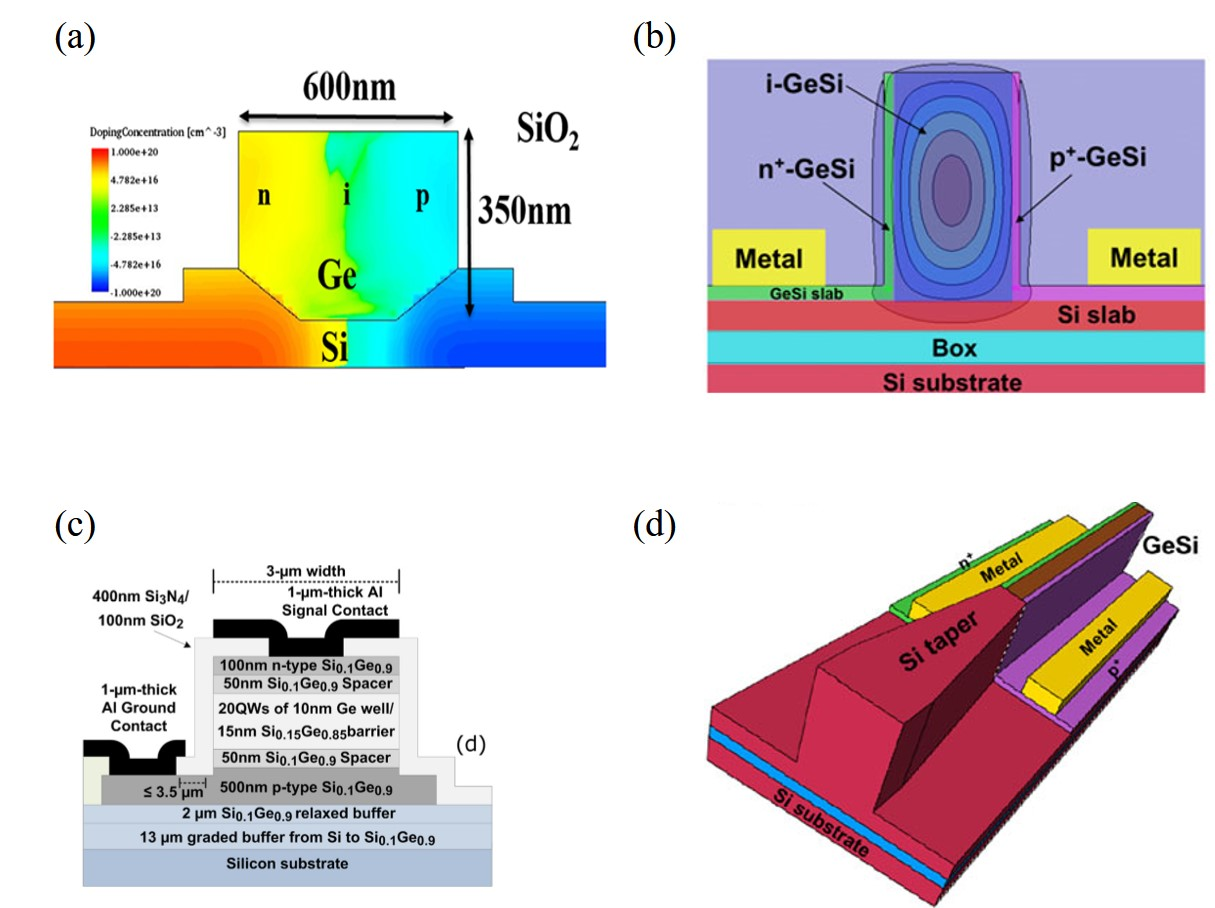
\includegraphics[width=12cm]{./Pictures/fig_ge_mod.jpg}
	\caption{ (a) 硅基锗光调制器\cite{Srinivasan201656};(b)硅基锗硅光调制器\cite{Dazeng2013high};(c)硅基锗硅多量子阱光调制器\cite{chaisakul201223};(d)硅波导和锗硅光调制器的耦合结构\cite{Dazeng2013high}}
	\label{fig_ge_mod}
\end{figure}
\subsection{硅基石墨烯光调制器}
石墨烯自从2004年被英国的研究人员发现\cite{novoselov2004electric},就在各个领域内被广泛应用。硅基石墨烯光调制器首次由是美国伯克利大学张翔小组实现,结构如图\ref{sil_graphene_mod}(a)所示,实现了小信号的3dB调制带宽达到了1.2 GHz.虽然首次展示的硅基石墨烯光调制器的速度受到器件的电容和电阻制约,但是石墨烯光调制器具有结构紧凑(40 $\mu m$),插入损耗低(2.4 dB),光学带宽大(>180 nm)的特点。随后很多研究人员,投入到高速石墨烯光调制器的研究中。
{
	\begin{table}[htb]
		\zihao{5}
		\caption{硅基石墨烯光调制器。EAM: Electro-absorption Modulator;EOM:Electro-optic Modulator;Term:Terminates}
		\label{sil_graphene_mod}
		\centering
		\begin{tabular}[t]{p{1.5cm}cp{0.8cm}p{1.2cm}ccccc}
			\hline
			调制原理 & 光学带宽 & 电极结构 & 调制区尺寸 & 调制速度 & 动态能耗 & 消光比 & 插入损耗 & 调制电压\\
			\hline
			Graphene EAM\cite{liu2011graphene} & >180 nm & LE  & 40 $\mu m$ & 1.2 GHz & - & 2.4 dB & - & 3 V\\
			Graphene EAM\cite{liu2012double} & -  & LE  & 40 $\mu m$ & 1 GHz & 1 pJ/bit & 6.5 dB & 4 dB & 3 V\\
			Graphene EAM\cite{hu2014broadband} & >80 nm & LE  & 50 $\mu m$ & 10 Gbps & 350 fJ/bit & 2.5 dB & 4 dB& 2.5 V\\
			Graphene Ring\cite{phare2015graphene} & - & LE (Term) & 30 $\mu m$ & 22 Gbps & 800 fJ/bit & - & -14 dB & 7.5 V\\
			\hline
		\end{tabular}
	\end{table}
}

表\ref{sil_graphene_mod}展示具有代表性的硅基石墨烯光调制器。双层石墨烯调制器,如图\ref{sil_graphene_mod}(b)所示,增加了光与石墨烯的相互作用,提高了的石墨烯光调制器的调制深度。随后,比利时的Imec提出的如图\ref{sil_graphene_mod}(c)所示的硅基石墨烯光调制器,通过合理设计硅波导的掺杂浓度和尺寸,以及石墨烯的和硅之间间隔,将调制器的调制速度提高到了10 Gbps\cite{liu2011graphene, hu2016broadband}。最近美国康奈尔大学的Lipson小组利用石墨烯调制微环的损耗从而影响微环的临界耦合系数,而微环的透射谱对临界耦合系数很敏感,进而实现30 GHz的石墨烯光调制器,结构如图\ref{sil_graphene_mod}(d)所示。该石墨烯的光调制器虽然制作于氮化硅的衬底,但是这种结构也可以应用于未来的高速硅基石墨烯光调制器。

\begin{figure}[htb]
	\centering
	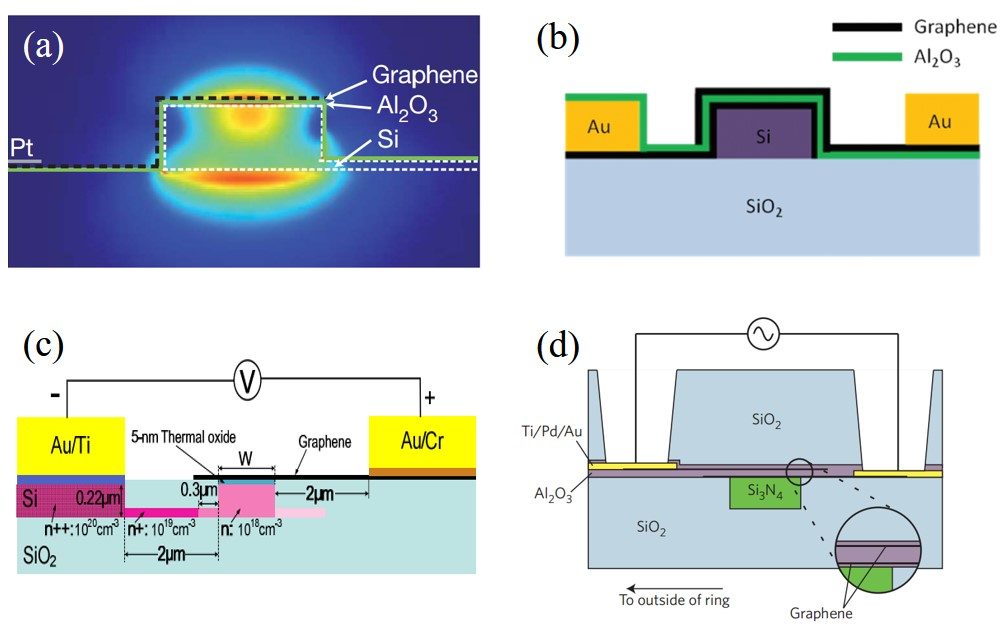
\includegraphics[width=12cm]{./Pictures/fig_graphene_mod.jpg}
	\caption{ (a) 硅基单层石墨烯光调制器\cite{liu2011graphene};(b)硅基双层石墨烯光调制器\cite{liu2012double};(c)硅基单层石墨烯光调制器\cite{hu2014broadband, hu2016broadband};(d)氮化硅基石墨烯光调制器\cite{phare2015graphene}}
	\label{fig_ge_mod}
\end{figure}

\subsection{硅基聚合物光调制器}
聚合物光调制器一直是研究的热点。目前世界上所有平台中的光调制器,调制速度最快的就是基于聚合物的光调制器。这个光调制速是在2002年由美国贝尔实验室实现的,调制带宽达到了1.6 THz\cite{lee2002broadband}。目前世界上硅基平台上的所有光调制器,调制速度最快的并且调制区域尺寸最小的也是基于聚合物的光调制器。这个光调制器是在2015年由瑞士苏黎世理工实现的,利用表面等离子体槽型波导,将光约束到纳米尺度,调制器的微波小信号3 dB带宽大于70 GHz,调制速度达到了72 Gbps,调制区域的尺寸只有6  $\mu m$。 聚合物除了速度快,其电光系数也很高,达到了230 pm/V \cite{palmer2014high},这与目前最好的纯硅光调制器的电光系数250 pm/V \cite{timurdogan2014ultralow}相当。
{
	\begin{table}[htb]
		\zihao{5}
		\caption{硅基聚合物光调制器。MZM:  Mach–Zehnder modulator;SOH: Silicon-Organic Hybrid Modulator}
		\label{sil_polymer_mod}
		\centering
		\begin{tabular}[t]{p{1.5cm}cp{1.2cm}ccccccc}
			\hline
			调制原理 & 电极结构 & 调制区尺寸 & 调制速度 & 动态能耗 & 消光比 & 插入损耗 & 调制电压\\
			\hline
			SOH\cite{palmer2014high} & LE  & 0.25 $mm$ & 40 Gbps & 420 fJ/bit & 9 dB & 6 dB & 2.1 V\\
			SOH\cite{palmer2014high} & TW  & 1.0 $mm$ & 40 Gbps & - & 8.9 dB & 6 dB & 1.5 V\\	
			SOH\cite{koeber2015femtojoule} & LE  & 1.0 $mm$ & 12.5 Gbps & 0.7 fJ/bit & -B & 6 dB & 1.5 V\\			
			Plamonic MZM\cite{haffner2015all} & LE  & 6 $\mu m$ & 72 Gbps & 25 fJ/bit & - & 8 dB & 6 V\\
			\hline
		\end{tabular}
	\end{table}
}
表\ref{sil_polymer_mod}展示了最近硅基聚合物光调制器的性能。传统的硅基聚合物光调制器是用槽型波导\cite{almeida2004guiding},将大部分光强约束到中间的聚合物中,如图\ref{fig_polymer_mod}(a)所示\cite{palmer2014high,liu2015recent}。传统的硅基聚合物光调制器利用MZI结构,如图\ref{fig_polymer_mod}(b)所示,速度能达到了40 Gbps。这类光调制器能耗最低达到0.7 fJ/bit.而最近采用表面等离子体槽型槽型波导结构,将调制器的尺寸从$10^3 \mu m$量级缩小到$\mu m$量级,速度也提高到了72 Gbps(受到测试仪器的带宽限制)\cite{haffner2015all}。这种调制器的器件结构和波导界面模场分布如图\ref{fig_polymer_mod}(c, d)所示。目前这种调制器阵列也被制作出来,展示了 4 $\times$ 36 Gbps的发射阵列\cite{heni2015high}。不过,硅基基于表面等离子体槽型波导的聚合物光调制器仍然需要进一步降低能耗,降低驱动电压,提高这类调制器的竞争力。
\begin{figure}[htb]
	\centering
	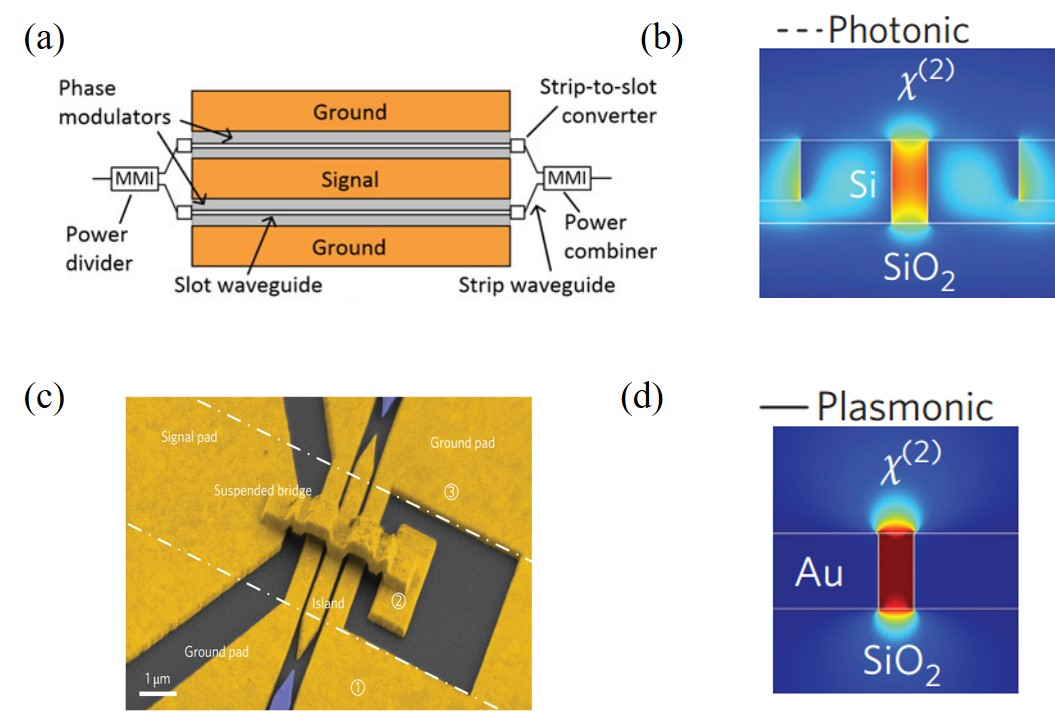
\includegraphics[width=12cm]{./Pictures/fig_polymer_mod.jpg}
	\caption{ (a) 硅基聚合物光调制器结构图\cite{palmer2014high};(b)硅基槽型波导模场分布\cite{palmer2014high};(c)硅基基于表面等离子体槽型波导聚合物型光调制器结构图\cite{haffner2015all};(d)硅基槽型表面等离子体波导模场分布图\cite{haffner2015all}}
	\label{fig_polymer_mod}
\end{figure}

\subsection{硅基其他电光材料光调制器}
目前主干网的光通信网络中,光调制器依旧大量采用铌酸锂(LiNbO\SB{3})光调制器。因此,很多研究人员尝试将铌酸锂等高电光系数的固体材料集成到硅平台上。表\ref{sil_others_mod}展示了最近将铌酸锂和钛酸钡(BaTiO\SB{3})薄膜混合集成到硅平台上,实现光调制器的性能。
{
	\begin{table}[htb]
		\zihao{5}
		\caption{硅基铌酸锂和钛酸钡的光调制器。}
		\label{sil_others_mod}
		\centering
		\begin{tabular}[t]{p{1.5cm}cp{1.2cm}ccccccc}
			\hline
			调制原理  & 电极结构 & 调制区尺寸 & 调制速度 & 动态能耗 & 消光比 & 插入损耗 & 调制电压\\
			\hline
			LiNbO\SB{3}\cite{chen2014hybrid} & LE  & 30 $\mu m$ & 9 Gbps & 4.4 pJ/bit & 3 dB & 5 dB & 5 V\\
			BaTiO\SB{3}\cite{xiong2014active} & LE  & 750 $\mu m$ & 300 Mbps & - & 3 dB & - & 6.6 V\\
			\hline
		\end{tabular}
	\end{table}
}
从表\ref{sil_others_mod}可以看出,这些材料的硅基光调制器性能还未完全开发。硅基铌酸锂光调制器采用铌酸锂薄膜放置到硅波导上表面,波导界面模场和器件结构图见图\ref{fig_othter_mod.jpg}(a,b)。这种光调制器最好的调制和能耗性能只有 9 Gbps和4.4 pJ/bit。最近高电光细数的钛酸钡被用于硅基光调制器,其电光系数达到了213 ± 49 pm/V \cite{xiong2014active},这种光调制器的结构和波导界面模场分布图如\ref{fig_othter_mod.jpg}(c-e)所示。虽然此光调制器速度目前只有 300 Mbps,通过合理设计电极仍然有提高的趋势。除此之外,压电陶瓷薄膜具有高电光系数(240 pm/V)也成功被溅射到了硅衬底上\cite{george2015lanthanide},这也是实现硅基新电光材料光调制器的新方案。未来将会有越来越多的新电光材料集成到硅平台上。
\begin{figure}[htb]
	\centering
	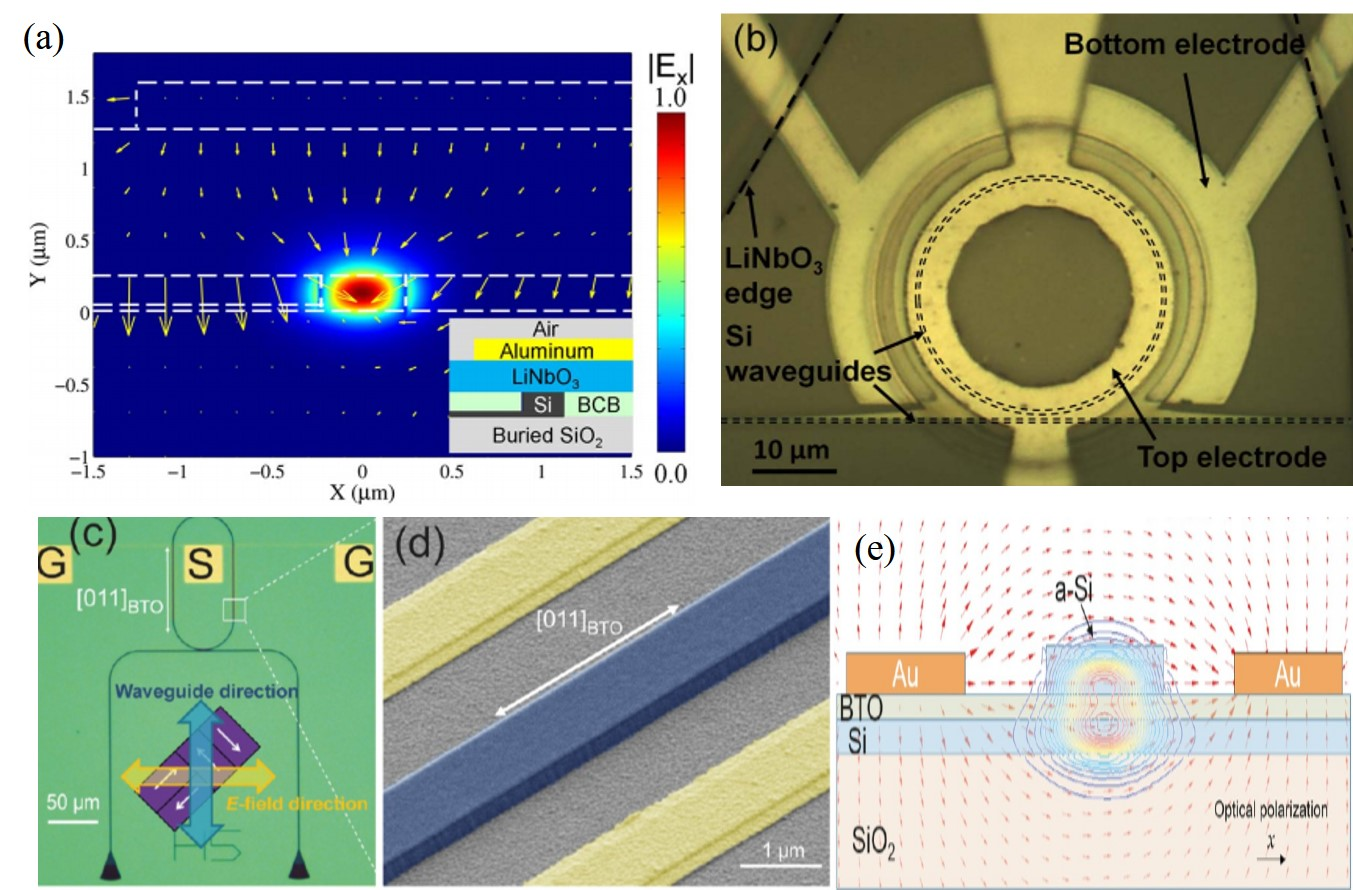
\includegraphics[width=12cm]{./Pictures/fig_othter_mod.jpg}
	\caption{ (a)硅基LiNbO3光调制器的截面和模场分布\cite{chen2014hybrid};(b)硅基LiNbO3光调器的俯视图\cite{palmer2014high};(c)硅基BaTiO3光调器的俯视图\cite{xiong2014active};(d)硅基BaTiO3光调器的局部放大图\cite{xiong2014active};(e)硅基BaTiO3光调器波导截面的模场分布图\cite{xiong2014active}}
	\label{fig_othter_mod.jpg}
\end{figure}
\subsection{硅基混合集成III-V光调制器}
自从1984年贝尔实验的研究人员发现了III-V量子阱中有强烈的量子束缚Stark效应(Quantum Confined Stark Effect, QCSE),可以实现电吸收调制器调\cite{miller1984band, wood1984high}。到如今, InP衬底的电吸收光调制器速度不仅达到了100 Gbps,并且与III-V激光器单片集成到了一起\cite{chacinski2009monolithically, kazmierski2009100}。另外根据Kramers-Kronig,材料折射率虚部的变化也会影响材料折射率实部,电吸收调制器不仅能做强度调制器,也能做相位调制器。文献[\citenum{poirier2015inp}]中,研究人员展示了单片集成III-V激光器和III-V相位调制器,实现了100 Gbps的双极化正交相移键控(Dual Polarization Quadrature Phase-Shift Keying, DP-QPSK)调制的发射器\cite{poirier2015inp}。 除此之外,高速电吸收调制器还有一个独特用处,可以同时作为高速探测器\cite{miller1985electric}。基于电吸收调制器这个特点,实现了单片集成的光收发模块\cite{welstand1996dual,chen2016wavelength},单片集成的光电光转化的微波发生器\cite{zhou2014compact}。

将III-V和Si混合集成在一起,一直是研究人员的梦想。可是III-V和Si的晶格具有8.1\%的不匹配程度,在Si上无法完美长出大面积III-V晶体。最近在硅基上虽然可以通过利用缓冲层和限制缺陷扩展的结构,外延生长InP的纳米线,实现了光泵浦激光器\cite{wang2015room},但是距离直接生长出III-V量子阱结构还差距很远。因此,目前是研究人员还是采用键合的方式将III-V和Si混合集成在一起,利用III-V直接带隙的特点,实现在硅基上电泵浦激光器,高速电吸收调制器,高速光探测器和半导体放大器\cite{liang2010hybrid,roelkens2010iii,liang2010recent,duan2014hybrid}。

\begin{figure}[htb]
	\centering
	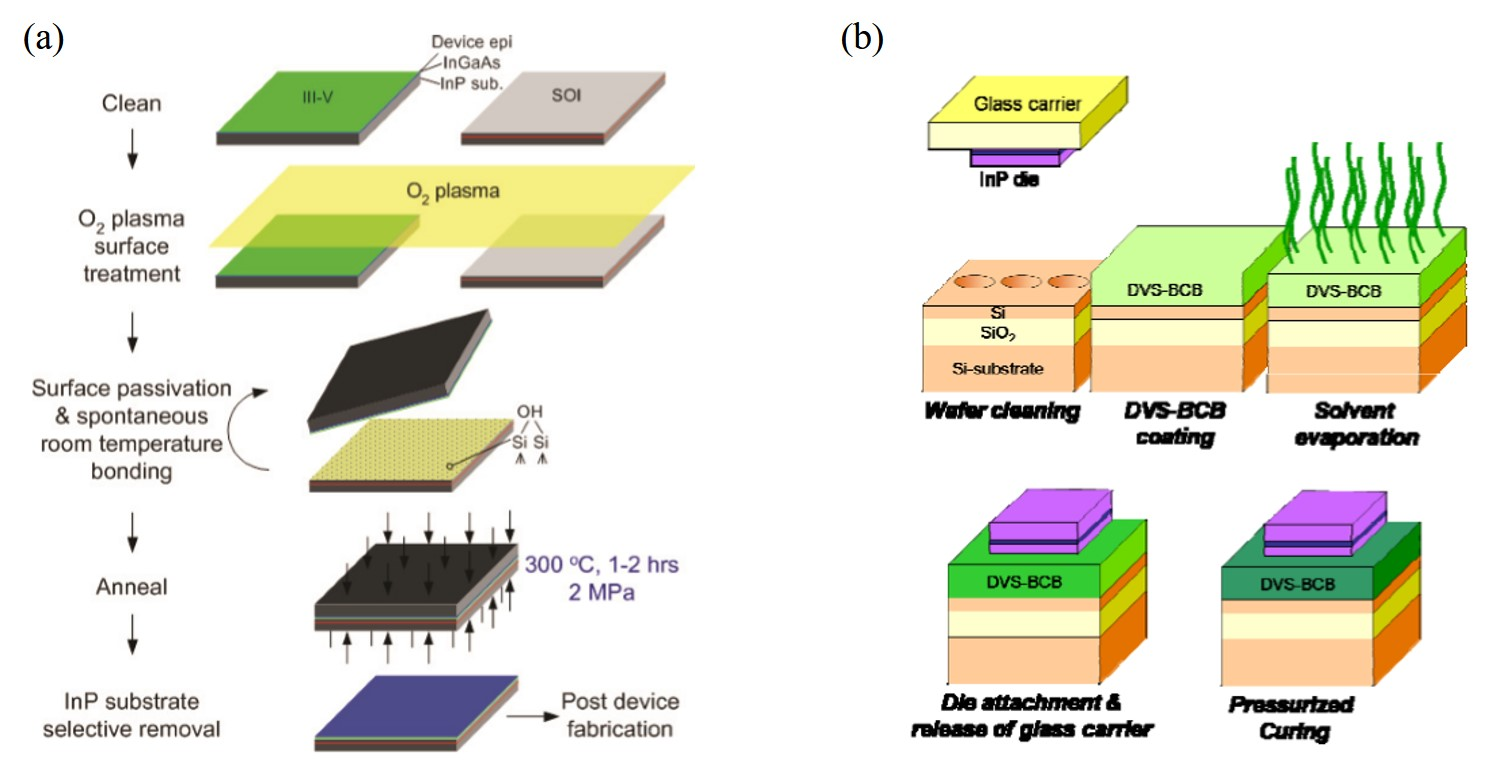
\includegraphics[width=14cm]{./Pictures/fig_bonding_methods.jpg}
	\caption{ (a) III-V和Si直接键合的工艺流程 \cite{liang2010hybrid, roelkens2010iii};(b) III-V和Si粘贴键合的工艺流程 \cite{liang2010hybrid, roelkens2010iii}}
\label{fig_bonding_methods}
\end{figure}

目前,有两种主流键合方式将III-V和Si混合集成在一起。第一种方式是III-V/Si直接键合,具体流程如图\ref{fig_bonding_methods}(a)所示。在III-V和Si键合表面先用氧等离子体分别活化,然后再将III-V和Si贴合,放置到300摄氏度的高压环境中退火。这种方法最早是瑞典的乌普萨拉大学的研究人员提出\cite{pasquariello2002plasma},而后经由美国加州大学圣塔芭芭拉分校的研究人员进一步优化\cite{liang2010hybrid},解决了键合表面产生气体的问题,不仅实现了第一个硅基混合集成的电泵浦III-V激光器\cite{fang2006electrically},也实现了第一个硅基混合集成的电吸收调制器\cite{kuo2008high}。第二种方式是III-V/SI粘贴键合,具体流程如图\ref{fig_bonding_methods}(b)所示。在III-V和Si表面中间添加一层粘贴剂,将它们紧密地键合在一起。虽然有很多种聚合物可以作为III-V和Si的粘贴剂,但是这种粘贴剂不仅不需要足够的粘贴强度,还需要厚度需要小于100 nm,便于光在硅波导和III-V波导之间的耦合。比利时根特大学的研究人员,利用稀释后的DVS-BCB(divinylsiloxane-bisbenzocyclobutene)聚合物实现了III-V和Si中间的粘贴层小于100nm\cite{liang2010hybrid, roelkens2010iii}。基于III-V/SI粘贴键合的混合集成平台上也同样实现了激光器,电吸收调制器等器件\cite{roelkens2015iii}。

\begin{figure}[htb]
	\centering
	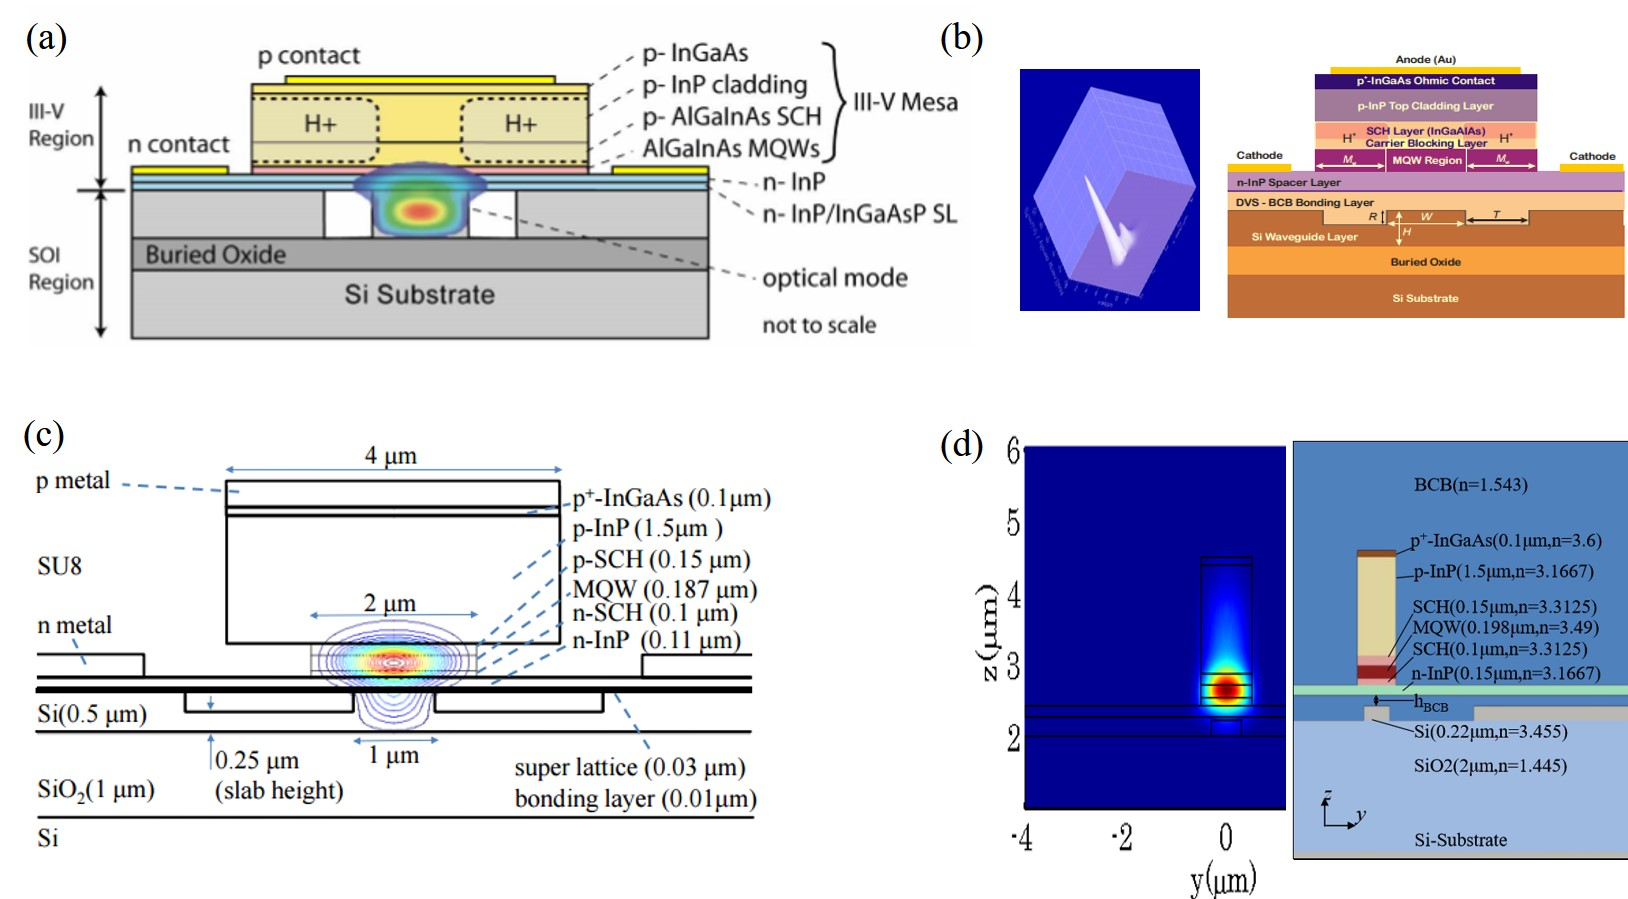
\includegraphics[width=12cm]{./Pictures/fig_hybrid_wg_cross.jpg}
	\caption{ (a) III-V/Si直接键合的混合集成波导截面结构和模场分布图\cite{fang2006electrically};(b) III-V/Si粘贴键合的混合波导模场分布图(左)和截面结构图(右)\cite{stankovic2010evanescently};(c) 用于调制器的III-V/Si直接键合的混合集成波导截面结构和模场分布图\cite{tang201150};(d) 用于调制器的III-V/Si粘贴键合的混合集成波导截面结构和模场分布图}
	\label{fig_hybrid_wg_cross}
\end{figure}

III-V/Si直接键合相比III-V/Si粘贴键合,III-V和Si之间的间隔更为紧密。图\ref{fig_hybrid_wg_cross}(a)展示了III-V/Si直接键合的混合集成波导截面结构和模场分布图,可以看到大部分光场集中在硅波导中,有部分倏逝波耦合到了III-V波导中。III-V/Si粘贴键合下,虽然他们之间的间隔相比而言比较远,但是由于粘贴剂的存在,对III-V和Si表面的粗糙度和洁净度容忍度更大\cite{gunther2007}。图\ref{fig_hybrid_wg_cross}(b)展示了III-V/Si粘贴键合的混合集成波导截面结构和模场分布图,光场也是大部分集中在硅波导中。不过,对于调制器而言,器件的尺寸越小,器件的电容就会越小,微波电极的损耗也越小,调制速度就会越快,因此需要将光大部分集中到III-V波导中,提高调制效率。图\ref{fig_hybrid_wg_cross}(b, c)分别展示了III-V/Si直接和粘贴键合平台下,调制器波导截面结构和模场分布图,可以两者结构中,通过减小硅波导的宽度,将光场大部分集中在III-V波导中,从而提高单位长度的调制效率,减少调制器尺寸。

硅基混合集成III-V光调制器自从2008年实现以后,性能逐年提高,电极种类囊括了图\ref{fig_mod_ele_type}中的四类,光学结构包含了图\ref{fig_mod_opt_type}中的三类。从表\ref{sil_IIIV_mod}中可以看出,调制速度最快的是采用TW和STLE结构的,速度到了50 Gbps,并且STLE电极的电光调制3 dB带宽达到了74 GHz\cite{tang2012over},这个调制速度和纯硅基光调制器的调制速度相当。最小尺寸的硅基混合集成III-V光调制器是采用图\ref{fig_mod_opt_type}中的第四种结构,基于调制微环的损耗,从而调制谐振波长的光强。该器件的示意图和实际器件如图\ref{fig_eam_ring}所示\cite{Srinivasan2012micro}。它直径24 $\mu m$的尺寸与纯硅基光调制器相比,还是偏大。在表中,我们也增加了自己最近的研究成果,实现了驱动电压只要50 mV, 动态功耗0.29 fJ/bit的电吸收光调制器。这种低驱动电压,低能耗的硅基混合集成III-V光调制器是目前所有光调制器中,驱动电压最低一类,并且在同样最低驱动电压下,实现了目前最大的消光比。除此之外,硅基混合集成的III-V电吸收调制器具有双工作模式,可以作为高速光探测器。凭借电吸收调制器的这种特性,我们展示了单片集成的光收发模块\cite{chen2016wavelength}。
{
	\begin{table}[htb]
		\zihao{5}
		\caption{硅基混合集成III-V光调制器研究进程。}
		\label{sil_IIIV_mod}
		\centering
		\begin{tabular}[t]{p{2cm}p{1cm}p{1cm}p{1.2cm}cccp{1cm}c}
			\hline
			键合方式  & \tabincell{c}{工作 \\ 方式} &\tabincell{c}{电极 \\ 结构}  & \tabincell{c}{调制区 \\ 尺寸} & 调制速度 & 动态能耗 & 消光比 & \tabincell{c}{插入 \\ 损耗} & 调制电压\\
			\hline
			直接键合\cite{kuo2008high} & EAM & LE & 250 $\mu m$ & 10 Gbps & - & 10 dB & 3 dB & 0.82 V\\
			直接键合\cite{tang201150} & EAM & TW & 100 $\mu m$ & 50 Gbps & 400 fJ/bit & 8.8 dB & 5 dB & 2 V\\
			直接键合\cite{tang2012over} & EAM & STLE & 100 $\mu m$ & 50 Gbps & 484 fJ/bit & 9.6 dB & 5 dB & 6.6 V\\
			直接键合\cite{tang2012energy} & EAM & LE & 100 $\mu m$ & 40 Gbps & 20 fJ/bit & 5 dB & 9 dB & 0.5 V\\
			直接键合\cite{chen2011forty} & EOM & CLTWE & 500 $\mu m$ & 40 Gbps & - & 6 dB & 9 dB & 4 V\\
			直接键合\cite{Srinivasan2012micro} & \tabincell{c}{EOM\\(Ring)} & LE & 24 $\mu m$ & - & 60 fJ/bit & - & - & 4 V\\
			粘贴键合\cite{fu20155} & EAM & LE  & 100 $\mu m$ & 28 Gbps & 200 fJ/bit & 5 dB & 1.2 dB & 2.4 V\\
			\tabincell{c}{粘贴键合 \\ (本论文工作)} & EAM & LE  & 80 $\mu m$ & 1.25 Gbps & 0.29 fJ/bit & 6.3 dB & 5 dB & 0.05 V\\
			\hline
		\end{tabular}
	\end{table}
}

\begin{figure}[htb]
	\centering
	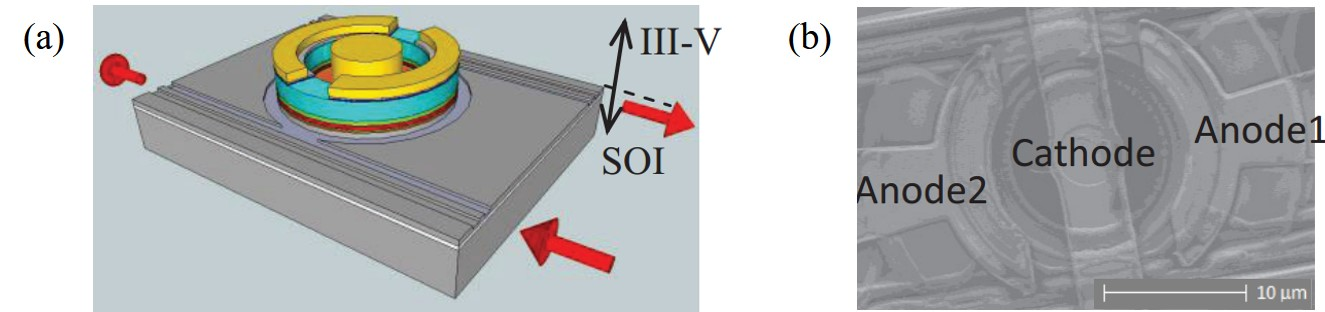
\includegraphics[width=12cm]{./Pictures/fig_eam_ring.jpg}
	\caption{ (a, b) 硅基混合集成III-V微环型光调制器的结构示意图和器件实际图\cite{Srinivasan2012micro}}
	\label{fig_eam_ring}
\end{figure}

\section{本论文的内容和创新点}
本论文主要分析讨论两种硅基光调制器。第一种是硅基混合集成III-V电吸收光调制器,第二种是纯硅基光调制器。对于第一种电吸收光调制器,我们的目标是降低驱动电压,减小能耗,缩小尺寸,以便提升器件的集成度,为日后半导体驱动电路和光器件单片集成提供基础。接着,我们充分利用电吸收调制器双工作模式,即调制器也可以作为高速探测器的特点,结合硅基无源器件,尝试在单个硅片上构建包含波分复用系统的光收发模块。对于第二种纯硅基光调制器,我们的目标是设计拥有新型光学结构的光调制器,实现在拥有大的光学带宽的同时,保持小的调制区域尺寸。

\subsection{本论文的章节安排}
第一章首先总结了硅基光电子集成技术的发展历史,以及目前最新的发展状况。然后着重介绍了硅基光调制器的性能指标,以及目前实现硅基光调制器的光学结构和电极结构。随后详细介绍了硅基上利用不同材料实现光调制器的原理,发展现状,性能指标,以及他们的优缺点。

第二章介绍了硅基混合集成III-V波导中两方面的设计。第一方面是量子阱结构的设计。首先介绍了用于电吸收光调制器量子阱结构的计算仿真方法,然后介绍了利用退火算法设计量子阱结构的思路。并且提供了利用退火算法设计偏振不敏感电吸收光调制器的量子阱结构的例子。第二方面是波导尺寸的设计,分析了混合集成III-V波导中矩形波导和蘑菇型波导尺寸的变化对光波和微波的影响,以及对调制速度的影响。

第三章介绍了硅基混合平台中,光从硅波导模式耦合到混合集成III-V波导模式的结构的设计。首先,我们分析了实现硅波导模式到混合集成III-V波导模式耦合的难点在于混合集成III-V波导中的高阶模式在耦合过程中容易被激发出来。为了解决这个问题,我们将耦合结构分成三段,逐渐将光耦合到最后的模式,从而减少激发出高阶模式。我们利用三维时域有限元差分(3D FDTD)的方法分别优化三个区域的耦合结构。接着,我们将优化后的三个区域组合成最终结构。随后我们分析了加工误差对耦合结构的影响。最后,我们设计了用电子束曝光机制作这种紧凑耦合结构的方案。

第四章介绍了低驱动电压硅基混合集成III-V光调制器的研制。首先解释了能带填充效应对量子阱激子吸收峰的影响和基于这种现象的电吸收调制器的性能。然后,我们详细介绍了设计和制作硅基混合集成III-V光调制器的工艺步骤。接着,在搭建的测试光调制器的高速平台上,对其进高速性能的测试。 随后,介绍了硅基混合集成III-V光调制器也可以作为高速光探测器。我们同样其进行高速性能测试。接着,我们展示了单片混合集成整列波导光栅,高速调制器,高速探测器的的光收发模块的测试结果。

第五章介绍了基于可调反射镜和微环结构的新型纯硅基光调制器。首先,介绍了微环内部反射率对微环透射谱的影响。然后分析了可调反射镜的工作原理。最后分析了新型纯硅基光调制器的工作性能。

第六章总结了本论文的内容的,并且也对后期的工作和未来的硅基光调制器的发展方向进行了讨论和展望。

\subsection{本论文的主要创新点}
本论文利用快速退火算法,简化了设计III-V量子阱结构多参数的问题。我们进一步展示了通过合理设计权值函数,可以设计用于偏振不敏感电吸收光调制器的量子阱结构的例子。

本论文设计了紧凑的硅波导和混合集成III-V波导的光耦合结构。该结构是基于220 nm厚的SOI平台,利用三段式锥形结构(Taper),将硅波导中的光缓慢地耦合到混合集成III-V波导中,从而避免在混合集成III-V波导中高阶模式的激发,从而实现长度只有8 $\mu m$的耦合结构,是目前文献报道中最紧凑的耦合结构。这个耦合结构的光学带宽具有100 nm以上,耦合效率都达到了95\%。随后,我们探索了用电子束曝光机制作这种紧凑耦合结构的方案。

本论文设计,制作,测试了硅基混合集成III-V电吸收光调制器,并且在世界上首次利用能带填充效应下量子阱中激子吸收峰的漂移,实现电吸收光调制器。第一次实现了电吸收光调制器在80  $\mu$m的长度下,驱动电压值只需要50 mV,动态能耗只有0.29 fJ/bit,于此同时,动态消光达到6.3 dB,调制速率达到1.25 Gbps。基于能带填充效应的电吸收调制器给了一种设计低驱动电压,低功耗,小尺寸的调制器的全新思路。

本论文借助于电吸收调制器在反偏电时既是调制器也是探测器的双工作状态的特点,首次展示了集成两个级联的整列波导光栅,高速调制器,高速探测器的单片硅基混合集成的光收发模块。目前,单个信道的收发传输速率为1.5~Gbps。 

最后,本论文首次提出了基于可调反射镜和微环结构的新型纯硅基光调制器。我们利用微环的透射谱对其内部反射率敏感的特点,通过在微环中引入片上集成的可调反射镜,通过调制可调反射镜的反射率,实现了输出光强度的调制。这种光调制器既有马赫-曾德尔光调制器大光学带宽的特点,也有微环调制器结构紧凑的特点。该设计的调制器相位调制区域只有20 $\mu$m,驱动电压只需要1.22 V,3 dB调制带宽将达到67 GHz。这种新结构不仅可以用于纯硅基光调制器,也可以用于硅基其他电光材料的光调制器。






\chapter{硅基混合集成III-V波导}
\section{量子阱结构的设计}
本论文的硅基混合集成III-V光调制器是基于多量子阱(Multiple Quantum Well, MQW)的电吸收效应,这个效应也被成为量子束缚Stark(Quantum Confined Stark Effect, QCSE)现象。而对于块状材料,电吸收效应被称作Franz-Keldysh效应\cite{keldysh1958effect,franz1958einfluss}。Franz-Keldysh效应是指在外界电场的作用下,材料的能带发生倾斜,吸收峰往长波漂移,即能量低于导带和价带间隔的光子依旧能使电子从价带激发到导带。在激发的过程中,也需要考虑导带的空穴和价带的电子之间的库仑相互左右,而形成的激子。由于激子效应,吸收谱的末端处有强烈的吸收峰。对于块材料,激子效应只在没有偏压下才会明显。而在有偏压的情况下,电子和空穴受到外界电场的左右,互相分离,导致激子无法形成。对于量子结构,电子和空穴都被约束在有势垒的量子阱中。即使在外界电场的作用下,能带发生倾斜,电子和空穴在量子阱中的寿命仍然很长,依旧可以在吸收谱上观测到激子效应。另外由于量子阱中势垒的作用,电子和空穴都在分立的能级。而外界电场引起量子阱能带的倾斜,使电子和空穴分立能级的间隔缩小,从而使吸收峰快速往长波漂移。在量子阱中,这种在外界电压下,吸收峰快速往长波漂移,并且保持激子吸收的现象称之为量子束缚Stark(Quantum Confined Stark Effect, QCSE)现象\cite{miller1984band,miller1985electric}。因此,基于QCSE的电吸收光调制器具有驱动电压小,小尺寸的特点。

\begin{figure}[htb]
	\centering
	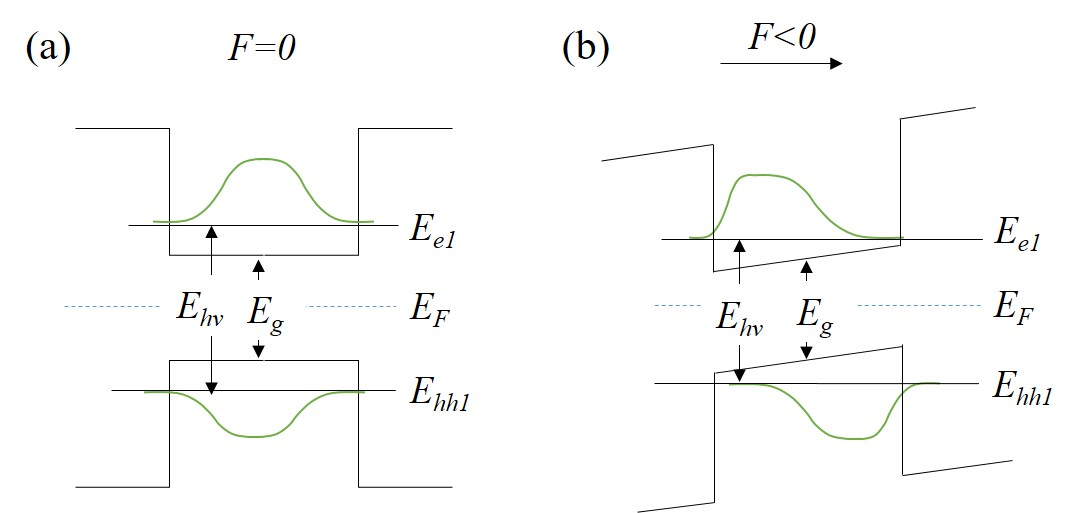
\includegraphics[width=14cm]{./Pictures/fig_ch2_band_lineup.jpg}
	\caption{ 量子阱的能带和波函数的示意图(a)有外界无电场下;(b)在外界电场的时候}
	\label{fig_ch2_band_lineup}
\end{figure}

图\ref{fig_ch2_band_lineup}(a)展示了没有外界偏压下量子阱的导带和价带,电子和空穴的波函数在空间上相互重叠,此时激子效应强度最大。当在外界电场的相互作用下,可以看到电子和空穴的分立能级的间隔变小,并且两者的波函数在空间上相错,此时激子效应的强度减弱。图\ref{fig_ch2_absorption_spec}(a,b)展示了实验测的不同偏振下量子阱的吸收谱随着外界电场的变化而变化\cite{chao1993momentum}。从中我们可以看出,外界电场使吸收谱往红移动,然后吸收谱边缘的激子吸收峰逐渐减弱,并且不同偏振下的吸收谱不同。图\ref{fig_ch2_absorption_spec}(c,d)展示了根据实验数据,里面计算得到的结果\cite{chao1993momentum}。可以看到理论和实验吻合的很好。关于量子阱中QCSE现象自从1984年在半导体量子阱材料被发现以来调\cite{miller1984band, wood1984high},依旧构建了多套完整的物理模型\cite{chuang1995physics}。下面,我们将介绍本论文采用的物理模型和计算方法。
\begin{figure}[htb]
	\centering
	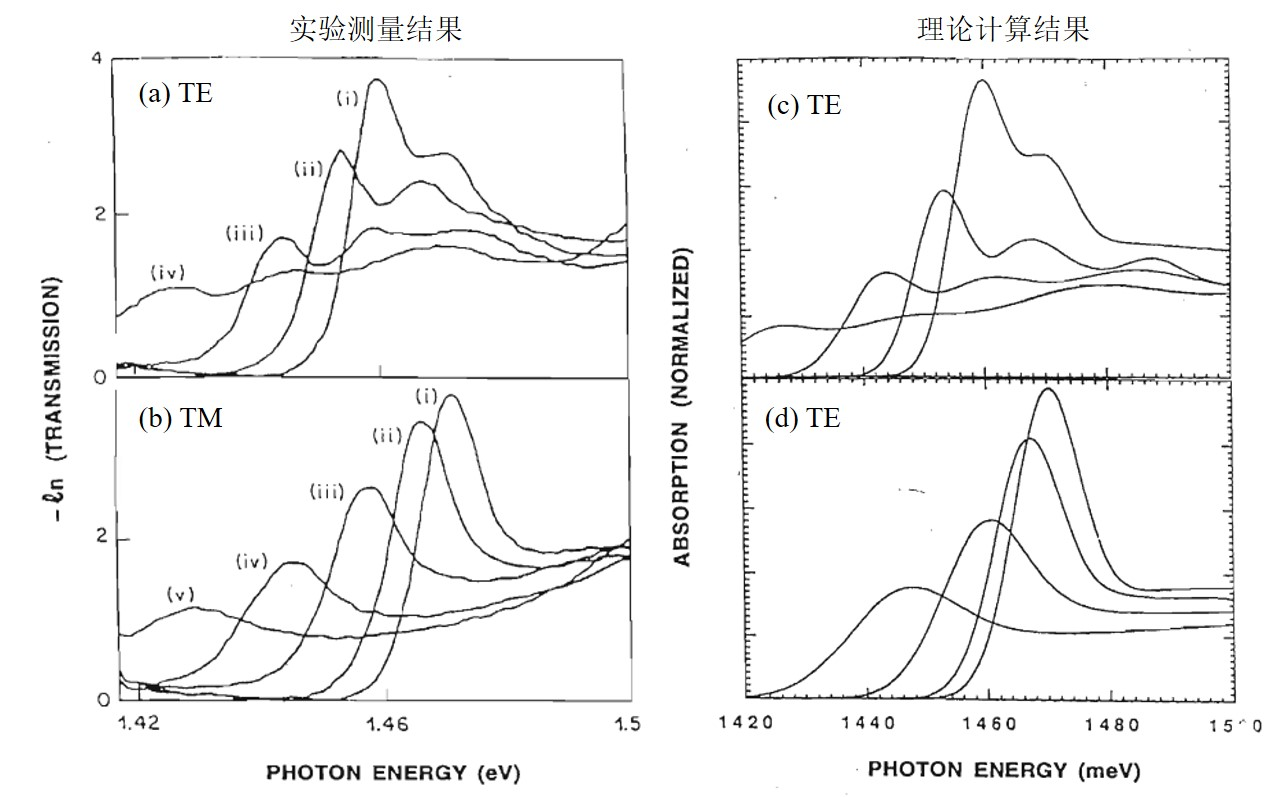
\includegraphics[width=14cm]{./Pictures/fig_ch2_absorption_spec.jpg}
	\caption{ (a,b) 实验测量的量子阱TE和TM偏振光的吸收谱\cite{chao1993momentum};(c,d) 理论计算的量子阱TE和TM偏振光的吸收谱\cite{chao1993momentum}}
	\label{fig_ch2_absorption_spec}
\end{figure}

\subsection{基本物理和数值计算}
目前计算量子阱的吸收谱商业上的软件只有一款昂贵的Harold EAM\cite{HarolEAM}软件。在此,我们采用文献[\citenum{chuang1995physics, mares1993modeling, roy1993modified, chuang1991exciton}]的方法,计算外界电场下的量子阱的吸收谱。计算吸收谱需要采用四个步骤,如图\ref{fig_ch2_flow_chart}(a)所示。通过第一步和第二布求解电子,空穴在外界下电场下的薛定谔方程\ref{Equ:Schro}得到本征能量$E$和波函数$\psi(z)$,如图\ref{fig_ch2_flow_chart}(b)所示。通过第三步和第四步求解出包含激子效应量子阱的吸收谱。
\begin{figure}[htb]
	\centering
	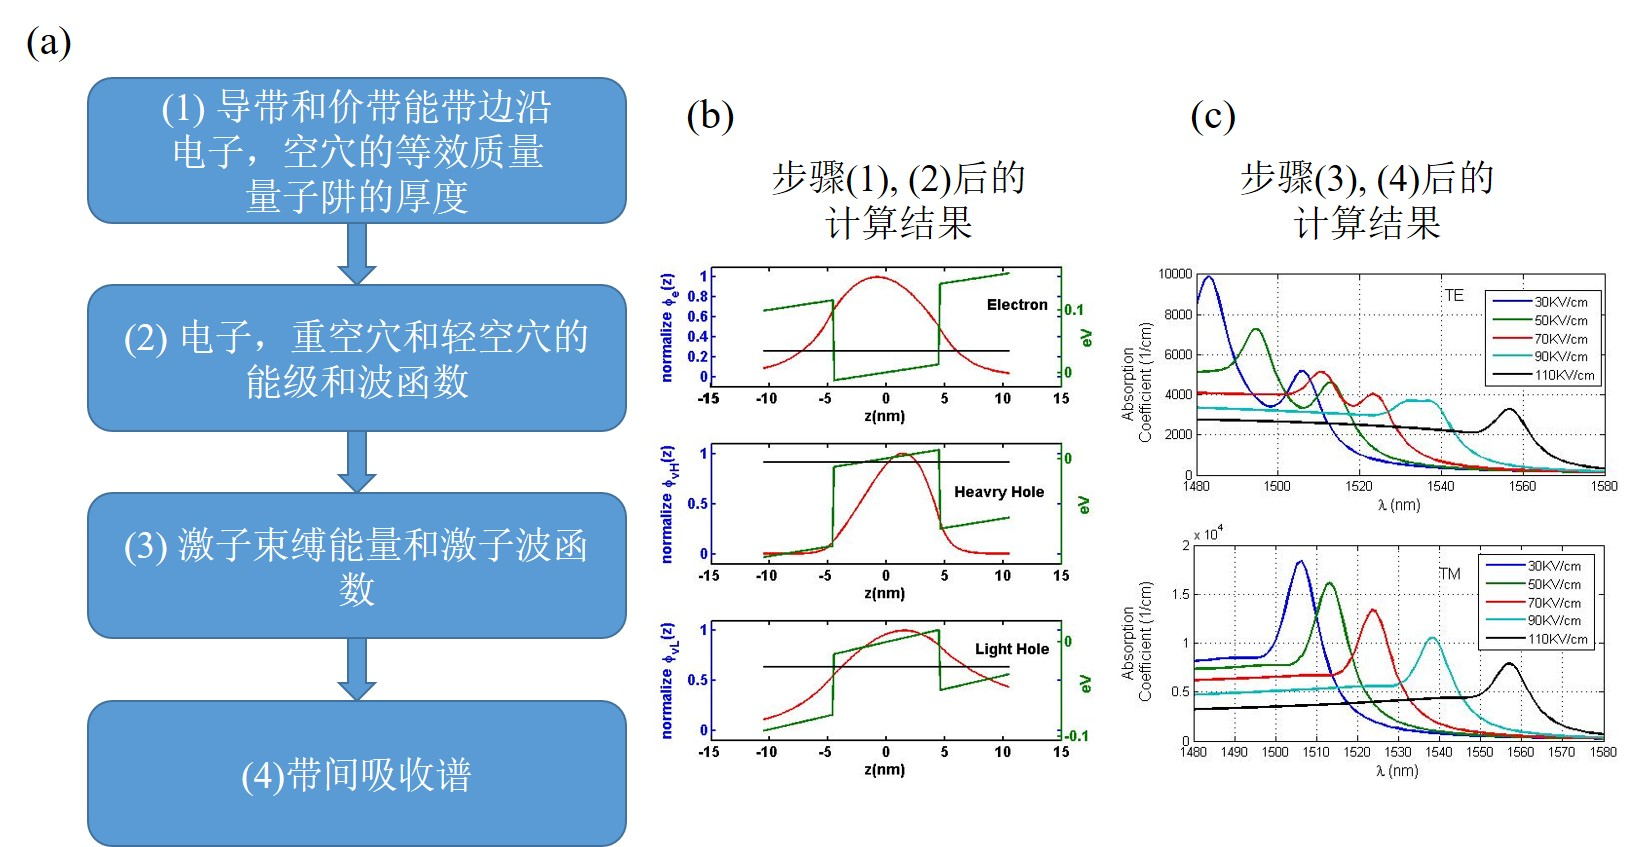
\includegraphics[width=16cm]{./Pictures/fig_ch2_flow_chart.jpg}
	\caption{(a)量子阱吸收谱的数值计算步骤;(b)第一和第二步的计算得到的电子,重空穴和轻空穴的能量和波函数;(c)第三和第四步计算得到的TE和TM偏振光的吸收谱}
	\label{fig_ch2_flow_chart}
\end{figure}

\begin{equation}
\label{Equ:Schro}
(\frac{\hbar^2}{2m}\Delta^2+V(z)+eFz)\psi(z)=E\psi(z)
\end{equation}
第一步计算材料的导带和价带的边沿结构。量子阱是由两种材料间隔排列而成。图\ref{fig_ch2_band_diagram}展示了在材料应力情况下量子阱能带边沿结构的变化\cite{chuang1995physics}。

\begin{figure}[htb]
	\centering
	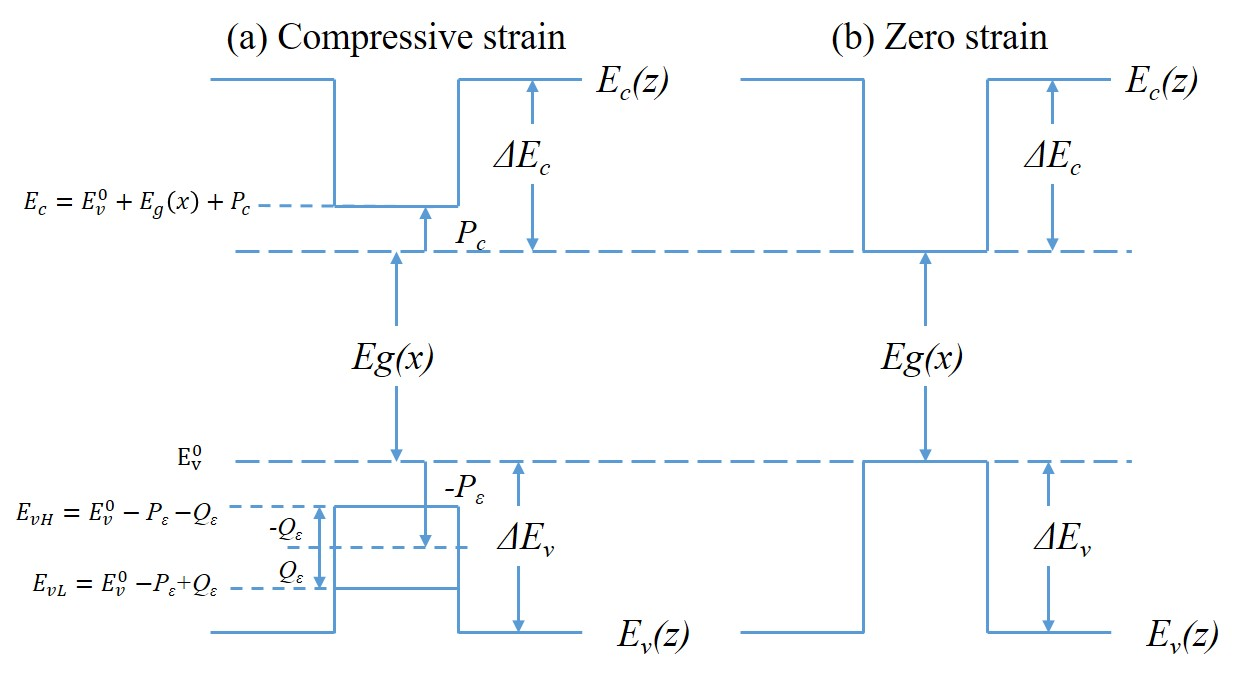
\includegraphics[width=14cm]{./Pictures/fig_ch2_band_diagram.jpg}
	\caption{有应力量子阱中的能带边沿图,(a)压缩应变;(b)张力应变}
	\label{fig_ch2_band_diagram}
\end{figure}

假设势阱中材料的晶格常熟为$a$,它在衬底晶格常数为$a_{0}$的材料上生长。那么我们可以用三个方向的应力来表式:
\begin{equation}
\label{Equ:exx}
\epsilon_{xx} = \epsilon_{yy} = \frac{a_{0}-a}{a}
\end{equation}
\begin{equation}
\label{Equ:ezz}
\epsilon_{zz} = -2\frac{C_{12}}{C_{11}}\epsilon_{xx}
\end{equation}
其中$C_{11}$和$C_{12}$是材料的弹性刚性常数(Elastic Stiffness Constants)。当$\epsilon_{zz}>0$时,材料处于压缩应变(Compressive Strain);当$\epsilon_{zz}>0$时,材料处于拉伸应变(Tensile Strain)。图\ref{fig_ch2_band_diagram}(a,b)展示了量子阱在有压缩应变和无应变情况下的能带的变化。通过比较,我们可以看到,导带上能带边沿$E_c$在受到压缩应变时,移动了$P_{c}$。表达式如下:
\begin{equation}
\label{Equ:Pc}
P_{c} = a_{c}(\epsilon_{xx}+\epsilon_{yy}+\epsilon_{zz})
\end{equation}
\begin{equation}
\label{Equ:Econ}
E_{c} = E_{v}^{0}(x)+E_{g}(x)+P_{c}
\end{equation}
其中$a_{c}$是导带的变形势能(Deformation Potentials),$E_v^0(x)$是材料在没有应变时导带的边沿,$E_{g}(x)$是材料没有应变时的导带和价带间隔,他们需要通过实验测试或者依旧材料的基本组分x查表拟合获得\cite{chuang1995physics,li2000material}。

在价带上,收到应变的影响,空穴分裂成重空穴和轻空穴,能带边沿分别是$E_{hh}$和$E_{lh}$。它们能带边沿的均值移动量是$P_{\epsilon}$,裂量是$Q_{\epsilon}$。具体表达式如下:
\begin{equation}
\label{Equ:Pe}
P_{\epsilon} = -a_{v}(\epsilon_{xx}+\epsilon_{yy}+\epsilon_{zz})
\end{equation}
\begin{equation}
\label{Equ:Qe}
Q_{\epsilon} = -\frac{b}{2}(\epsilon_{xx}+\epsilon_{yy}-2\epsilon_{zz})
\end{equation}
\begin{equation}
\label{Equ:Ehh}
E_{hh} = E_{v}^{0}(x)-P_{\epsilon}-Q_{\epsilon}
\end{equation}
\begin{equation}
\label{Equ:Elh}
E_{lh} = E_{v}^{0}(x)-P_{\epsilon}+Q_{\epsilon}
\end{equation}
其中$a_{v}$和$b$是变形势能。利用公式\ref{Equ:Econ},\ref{Equ:Ehh}、\ref{Equ:Elh}计算量子阱两种材料的能带边缘,就可以获得薛定谔方程中的电子,轻空穴和重空穴的势能$V(z)$。

在应力作用下,由于重空穴和轻空穴产的能带生劈裂,其等效质量,我们需要采用Luttinger parameters$\gamma_1, \gamma_2$计算。如下式所示:
\begin{equation}
\label{Equ:eff_mass_z}
\frac{m_{hh}^z}{m_0}=\frac{1}{\gamma_1-2\gamma_2}~~~~~~~~~~\frac{m_{lh}^z}{m_0}=\frac{1}{\gamma_1+2\gamma_2}
\end{equation}
\begin{equation}
\label{Equ:eff_mass_xy}
\frac{m_{hh}^{xy}}{m_0}=\frac{1}{\gamma_1+\gamma_2}~~~~~~~~~~\frac{m_{lh}^{xy}}{m_0}=\frac{1}{\gamma_1-\gamma_2}
\end{equation}
其中公式\ref{Equ:eff_mass_z}和公式\ref{Equ:eff_mass_xy}分别是计算垂直与量子阱方向(即z方向)和水平方向重空穴和轻空穴的等效质量\cite{eppenga1987new}。

我们用于硅基混合集成III-V电吸收光调制器的多量子阱中,单个量子阱的势阱(Well)和势垒(Barrier)分别是:In\SB{0.65}Al\SB{0.09}Ga\SB{0.26}As和In\SB{0.42}Al\SB{0.17}Ga\SB{0.39}As。从文献[\citenum{chuang1995physics,li2000material}],根据它们各个元素,再依据\ref{Equ:Econ},\ref{Equ:Ehh}、\ref{Equ:Elh}、\ref{Equ:eff_mass_z}、\ref{Equ:eff_mass_xy}式可以获得如下表\ref{QWmaterial}的量子阱材料数据。其中势阱受到了0.82\%的压缩应变,势垒受到了0.73\%的拉伸应变。
{
	\begin{table}[htb]
		\zihao{5}
		\caption{量子阱材料数据。E\SB{lh}:轻空穴的能带边沿;E\SB{hh}:重空穴的能带边沿;E\SB{c}:导带的能带边沿;$m_{lh}^z$:轻空穴z向等效质量;$m_{lh}^{xy}$:轻空穴xy向等效质量;$m_{hh}^z$:重空穴z向等效质量;$m_{hh}^{xy}$:重空穴xy向等效质量;$m_e$:电子等效质量;$m_0$:电子质量。}
		\label{QWmaterial}
		\centering
		\begin{tabular}[t]{ccccccccc}
			\hline
			类型  & E\SB{lh}(eV) & E\SB{hh}(eV) & E\SB{c}(eV) & $m_{lh}^z$ ($m_0$) & $m_{lh}^{xy}$ ($m_0$) & $m_{hh}^{z}$ ($m_0$) & $m_{hh}^{xy} $ ($m_0$) & $m_e$ ($m_0$)\\
			\hline
			Well & -6.7220 & -6.6695 & -5.9031 & 0.0374 & 0.1216 & 0.4874 & 0.0486 & 0.0457\\
			Barrier& -6.7573 & -6.8114 & -5.7680 & 0.0481 & 0.1498 & 0.5080 & 0.0621 & 0.0641\\
			\hline
		\end{tabular}
	\end{table}
}

第二步数值求解公式\ref{Equ:Schro}计算电子,重空穴和轻空穴在在一维势阱中的能级和波函数。在此我们采用的是基于传输矩阵的求解方法\cite{chuang1995physics}。首先我们将势能$V(z)+eFz$均匀分解很小的区域如图\ref{fig_ch2_divide_potential}所示。
\begin{figure}[htb]
	\centering
	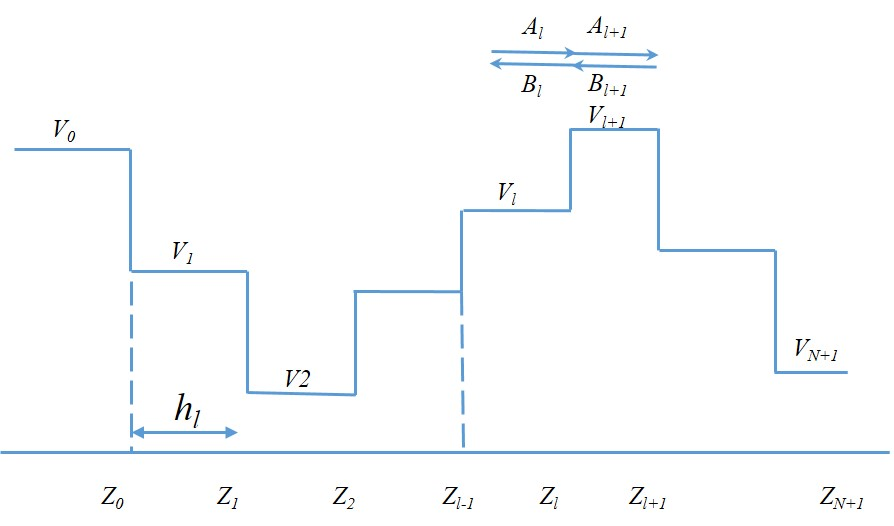
\includegraphics[width=12cm]{./Pictures/fig_ch2_divide_potential.jpg}
	\caption{将势能均匀划分成很小区域的示意图}
	\label{fig_ch2_divide_potential}
\end{figure}

假设在区域$l$,$z_{l-1} \leqslant z \leqslant z_{l}$,势能为$V_l$,粒子质量为$m_l$,那么其波函数$\psi(z)$的通解为:
\begin{equation}
\label{Equ:generalsolutionsch}
\psi(z) = A_le^{ik_l(z-z_l)}+B_le^{-ik_l(z-zl)}
\end{equation}
其中区域$l$的波数$k_l$可以用本征能量$E$来表示:
\begin{equation}
\label{Equ:kl}
k_l = \sqrt{\frac{2m_l}{\hbar^2}(E-V_l)}
\end{equation}
再利用每个区域边间上$\psi(z)$和$(1/m(z))d\psi(z)/dz$连续的条件,我们可以获得区域$l+1$的系数$A_{l+1}$和$B_{l+1}$与区域$l$的系数$A_l$和$B_l$的关系:
\begin{equation}
\label{Equ:ABrelation}
\begin{bmatrix}
A_{l+1}\\
B_{l+1}
\end{bmatrix} = \textbf{F}_{(l+1)l}\begin{bmatrix}
A_{l}\\
B_{l}
\end{bmatrix}
\end{equation}
其中$\textbf{F}_{(l+1)l}$可以表示为:
\begin{equation}
\label{Equ:Fdetail}
\textbf{F}_{(l+1)l} = \frac{1}{2}\begin{bmatrix}
(1+P_{(l+1)l})e^{ik_{l+1}h_l}&(1-P_{(l+1)l})e^{ik_{l+1}h_l}\\
(1-P_{(l+1)l})e^{-ik_{l+1}h_l}&(1+P_{(l+1)l})e^{-ik_{l+1}h_l}
\end{bmatrix}
\end{equation}
其中$P_{(l+1)l}$可以表示为:
\begin{equation}
\label{Equ:Pdetail}
P_{(l+1)l} = \frac{m_lk_{l+1}}{m_{l+1}k_{l}}
\end{equation}
因此,我们可以得到第一个区域系数$A_{0}$和$B_{0}$和最后一个区域系数$A_{N+1}$和$B_{N+1}$的关系:
\begin{equation}
\label{Equ:Fmulti}
\begin{bmatrix}
A_{N+1}\\
B_{N+1}
\end{bmatrix} = \textbf{F}_{(N+1)N}\textbf{F}_{N(N-1)}\cdots\textbf{F}_{21}\textbf{F}_{10}\begin{bmatrix}
A_{0}\\
B_{0}
\end{bmatrix}
\end{equation}
由于第一区域和最后区域波函数一般要衰减的,因此$A_0 = 0$,$B_{N+1} = 0$。另外我们将矩阵的连乘写成如下形式:
\begin{equation}
\label{Equ:Fsimple}
\textbf{F}_{(N+1)N}\textbf{F}_{N(N-1)}\cdots\textbf{F}_{21}\textbf{F}_{10} = \begin{bmatrix}
f_{11}&f_{12}\\
f_{21}&f_{22}
\end{bmatrix}
\end{equation}
因此公式\ref{Equ:Fmulti}可以写成如下形式:
\begin{equation}
\label{Equ:Fmulti}
\begin{bmatrix}
A_{N+1}\\
0
\end{bmatrix} = \begin{bmatrix}
f_{11}&f_{12}\\
f_{21}&f_{22}
\end{bmatrix}
\begin{bmatrix}
0\\
B_{0}
\end{bmatrix}
\end{equation}
因此,我们获得了求解借本征量能$E$的方程:
\begin{equation}
\label{Equ:sloveE}
f_{22}(E) = 0
\end{equation}
利用牛顿迭代法或者其他数值方法我们可以获得$E$的数值。然后公式\ref{Equ:kl},\ref{Equ:Pdetail},\ref{Equ:Fdetail}反推得到$\textbf{F}$。再假设$B_{0}$的数值,利用公式\ref{Equ:Fmulti},我们就可以得到每个区域波函数$\psi(z)$。最后,根据粒子在整个空间出现的概率为1,对波函数进行归一化。图\ref{fig_ch2_bias_wavefunction}分别展示了在没有偏压和2 KV/cm的偏压下,利用传输矩阵,计算得到的电子,重空穴,轻空穴的最低能级和对应波函数,其中量子阱势阱的宽度 $t_w = 11 ~nm$。在没有偏压下,电子和重空穴之间的能量间隔是$E_{e-hh} = 0.7997 ~eV$,当偏压为18~ KV/cm时,其间隔变为$E_{e-hh} = 0.7982~eV$,表明吸收峰红移了$\Delta E_{e-hh} = 1.5 ~meV$。电子和轻空穴在没有偏压和18 ~KV/cm下的能量间隔$E_{e-lh}$分别是$0.8649 eV$和$0.8597 eV$,红移量为 $\Delta E_{e-lh} = 5.2~ mV$。$\Delta E_{e-lh}$ 大于 $\Delta E_{e-hh}$是由于,如表\ref{QWmaterial}所示,轻空穴的等效质量少于重空穴,并且轻空穴的势垒和势阱的能带变差相比重空穴而言更小,因此轻空穴更容易受到势能变化的影响。从图\ref{fig_ch2_bias_18KV_wf}的最后一幅轻空穴的波函数图中可以看出,轻空穴即将突破量子阱势垒的束缚。当外界电场很强时,由于粒子会有部分从势阱里逃逸,此时波函数无法用公式\ref{Equ:generalsolutionsch}来表示,需要采用Airy方程表示此时波函数的通解\cite{chuang1991exciton}。
%\begin{figure}[htb]
%	\centering
%	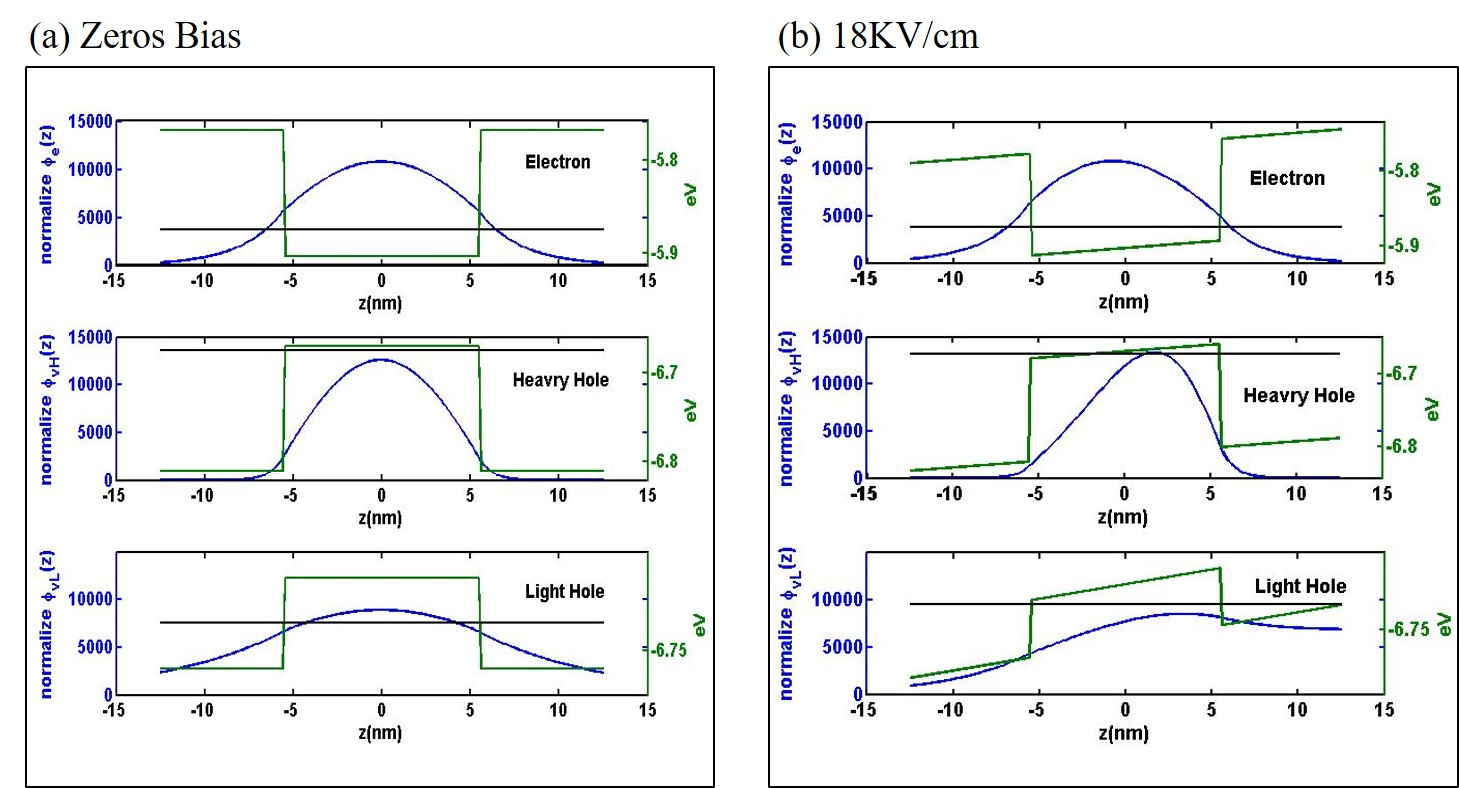
\includegraphics[width=16cm]{./Pictures/fig_ch2_bias_wavefunction.jpg}
%	\caption{在不同偏压下电子,重空穴和轻空穴能带边沿,波函数,能级的变化,(a)无电场;(b)电场强度为18~ KV/cm}
%	\label{fig_ch2_bias_wavefunction}
%\end{figure}

\begin{figure}[htb]
	\small
	\subfigure[0~KV/cm]{
		\begin{minipage}[]{0.5\textwidth}
			\centering
			\label{fig_ch2_bias_0KV_wf}
			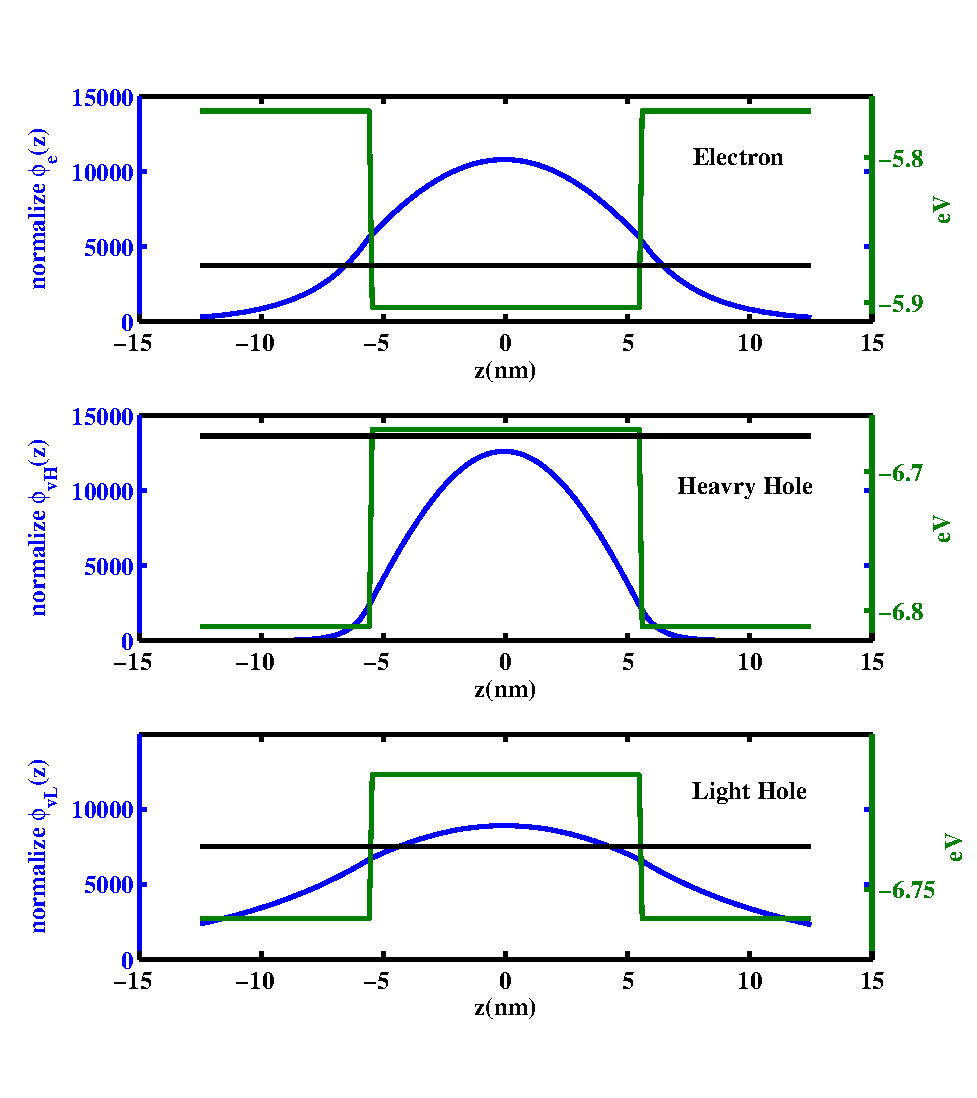
\includegraphics[width=8cm]{./Pictures/fig_ch2_bias_0KV_wf.eps}
		\end{minipage}}
	\subfigure[18~KV/cm]{
		\begin{minipage}[]{0.5\textwidth}
			\centering
			\label{fig_ch2_bias_18KV_wf} %% label for second subfigure
			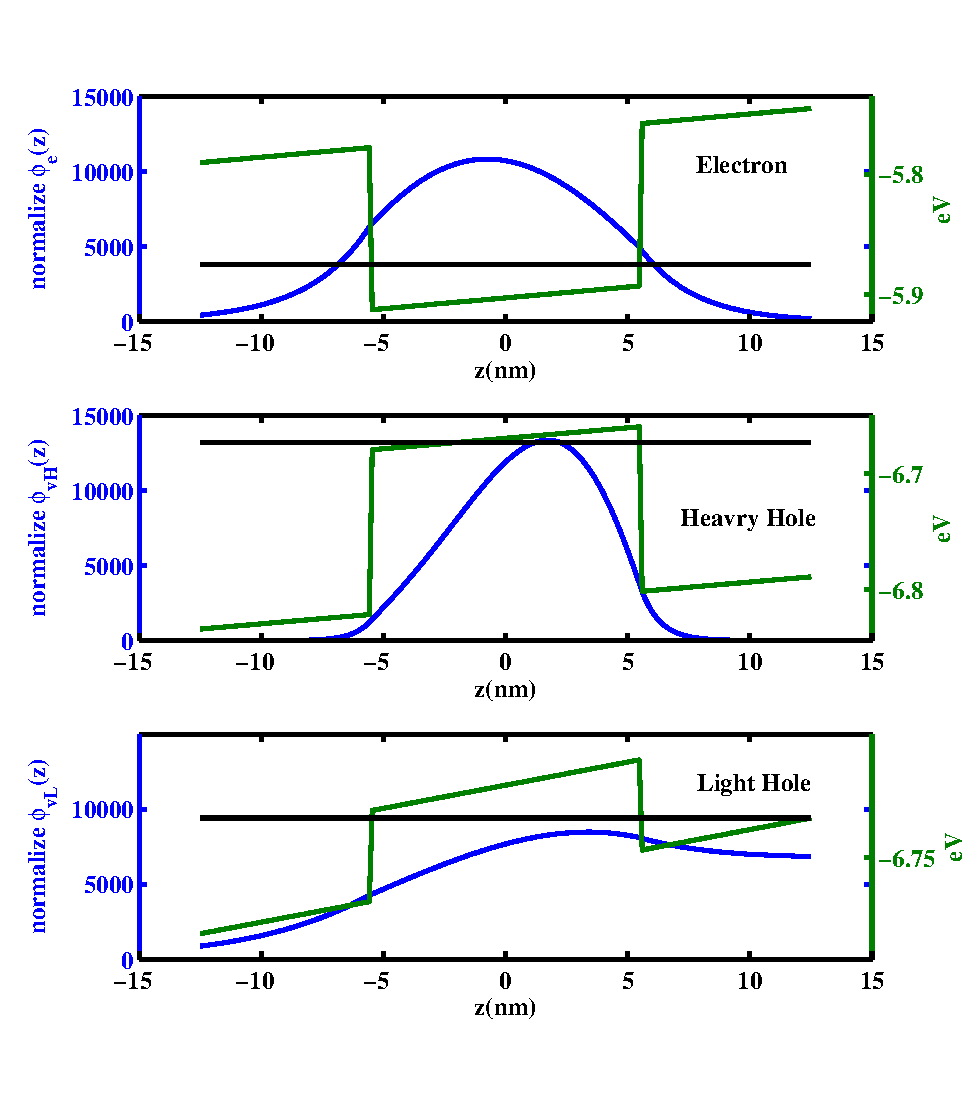
\includegraphics[width=8cm]{./Pictures/fig_ch2_bias_18KV_wf.eps}
		\end{minipage}}
	\caption{在不同偏压下电子,重空穴和轻空穴能带边沿,波函数,能级的变化}
	\label{fig_ch2_bias_wavefunction}	
\end{figure}
		
第三步求解激子的束缚能$E_B$和激子波函数$\psi(\rho)$。$\rho$是电子和空穴的xy平面上的距离。量子阱吸收谱的边缘处的能量$E_{e-h}$由能带间隔$E_g$,电子的能级$E_e$,空穴的能级$E_h$,激子束缚能$E_B$确定的,如下式所示:
\begin{equation}
\label{Equ:Eeh}
E_{e-h} = E_g + E_e + E_h + E_B
\end{equation}

求解$E_B$和$\psi(\rho)$需要解含电子空穴在库仑动能中的薛定谔方程\cite{mares1993modeling}。可以通过变法发求解这个方程\cite{miller1985electric, mares1993modeling}。最后可以转化为求解公式\ref{Equ:EB_lambda}的最小值问题。
\begin{equation}
\label{Equ:EB_lambda}
E_B(\lambda)=\frac{\hbar^2}{2\mu\lambda^2}-\frac{e^2}{4\pi\epsilon_r\epsilon_0}\int_{ - \infty }^{ \infty } {dz_e}\int_{ - \infty }^{ \infty } {dz_h	\left| \psi_e(z_e) \right|^2\left| \psi_h(z_h) \right|^2}\int_{ 0 }^{ \infty }{dq\frac{e^{-q\left| z_e-z_h \right|}}{\left[1+\left( \lambda q/2 \right) ^2 \right]^{3/2}}}
\end{equation}
其中$\lambda$是变分法中的变分参数。激子波函数$\psi(\rho)$可以用变分参数$\lambda$表示为:
\begin{equation}
\label{Equ:psirho}
\psi(\rho)=\sqrt{2/\pi}\left(e^{-\rho/\lambda}/\lambda \right)
\end{equation}

图\ref{fig_ch2_ex_abs1}和图\ref{fig_ch2_ex_abs2}展示了,在有激子和没有激子效应下,量子阱中$E_{e-hh}$与$E_{e-lh}$所对应的吸收峰边沿随外界电场的漂移。可以看出不考虑激子效应的吸收峰边沿比实际的吸收峰往短波偏,但是两者的吸收峰边沿在外界电压的变化下,都以二次函数的关系进行红移。可以总结出,激子的束缚能随外界电场的变化量远小于电子和空穴能级间隔的变化量。
\begin{figure}[htb]
	\centering
	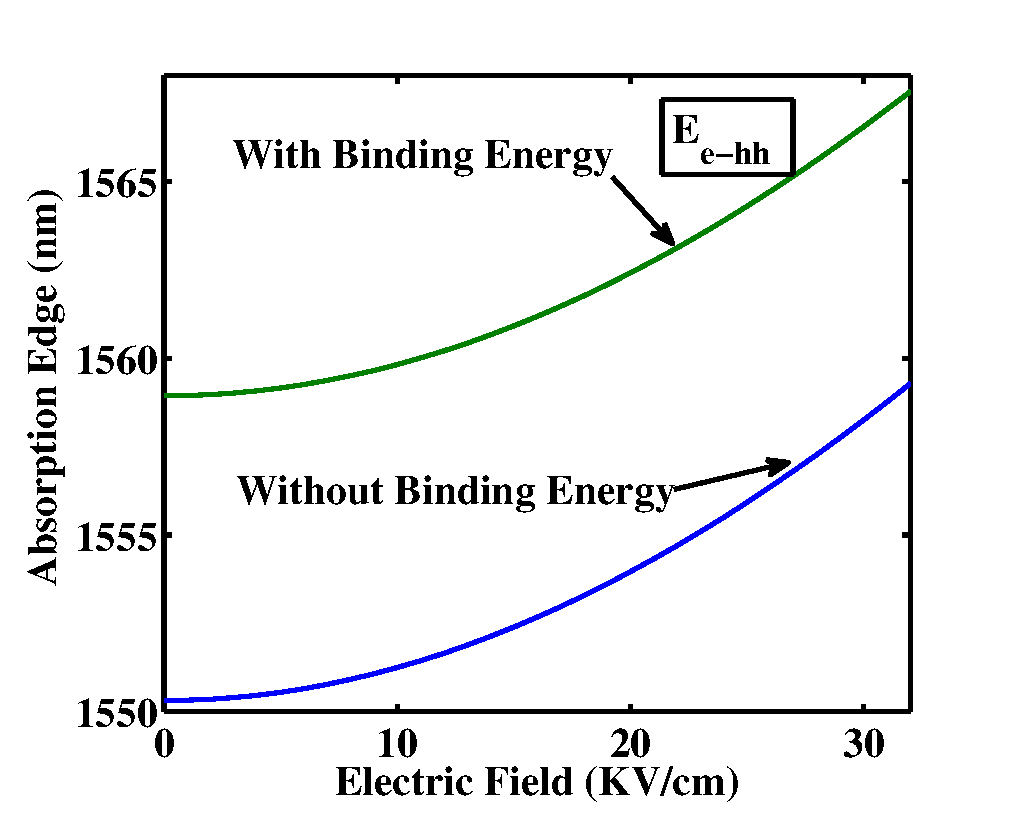
\includegraphics[width=12cm]{./Pictures/fig_ch2_ex_abs1.eps}
	\caption{$E_{e-hh}$所对应吸收峰边沿没有和存在激子效应下,随外界电场的变化}
	\label{fig_ch2_ex_abs1}
\end{figure}
\begin{figure}[htb]
	\centering
	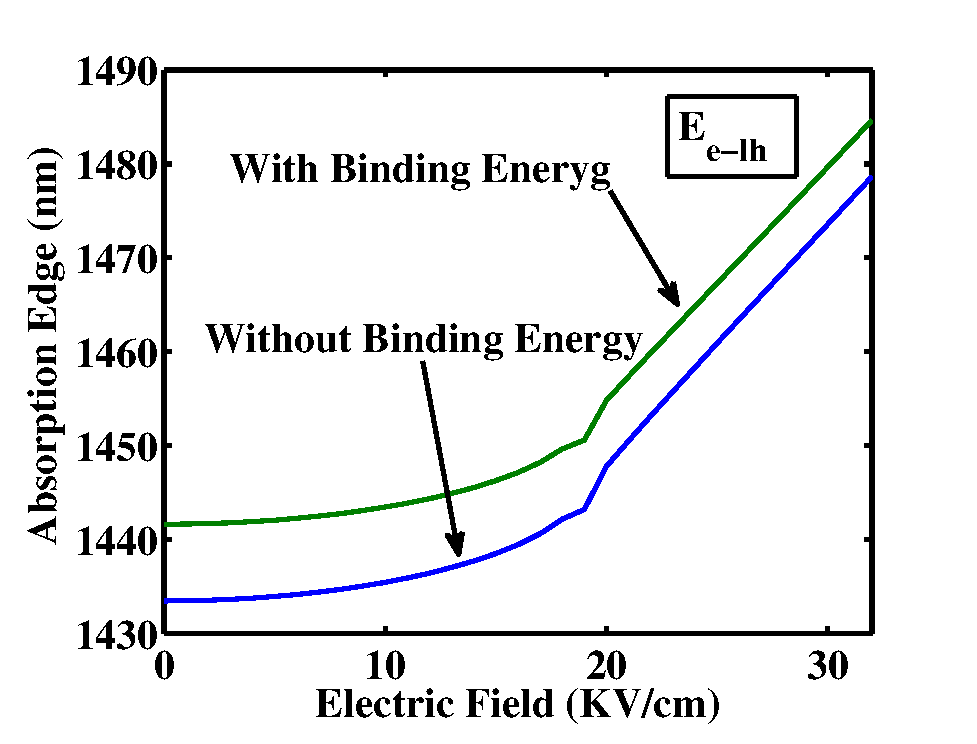
\includegraphics[width=12cm]{./Pictures/fig_ch2_ex_abs2.eps}
	\caption{$E_{e-lh}$所对应吸收峰边沿没有和存在激子效应下,随外界电场的变化}
	\label{fig_ch2_ex_abs2}
\end{figure}

第四步求解量子阱带间跃迁的吸收谱。带间电子能级$n$和空穴能级$m$的跃迁吸收谱可以简化成两个部分,第一个部分是带间连续跃迁导致的连续吸收谱,如公式\ref{Equ:continuumabs}所示;第二个部分是激子跃迁产生的激子吸收谱,如公式\ref{Equ:excitonabs}所示。
\begin{equation}
\label{Equ:continuumabs}
\begin{aligned}
\alpha(\omega) = &\frac{\omega \mu e^2}{n_rc\epsilon_0\pi m_0^2 L_p} \sum_m\sum_n\left| I_{nm} \right|^2\left| M_{AVG} \right|^2 \\ & \int_{0}^{\infty}\frac{dE~M(E)S_{nm}\Gamma}{(E_g+E_m+E_n+E)^2[(E_g+E_m+E_n+E-\hbar\omega)^2+\Gamma^2]}
\end{aligned}
\end{equation}

\begin{equation}
\label{Equ:excitonabs}
\alpha(\omega) = \frac{2\omega e^2 \hbar^2}{n_r c \epsilon_0 m_0^2 L_p} \sum_{mn}\frac{M(E)|M_{AVG}|^2|I_{nm}|^2|\psi(\rho = 0)^2|^2\Gamma}{(E_g+E_m+E_n+E_B)^2[(E_g+E_m+E_n+E_B-\hbar\omega)^2+\Gamma^2]}
\end{equation}
其中,$I_{nm}$是电子和空穴对应能级的波函数的重叠积分
\begin{equation}
\label{Equ:Imn}
I_{nm} = \left< \psi_n(z)|\psi_m(z)\right>,
\end{equation}
$|M_{AVG}| ^2$是布洛赫模式的平均矩阵量
\begin{equation}
\label{Equ:MAVG}
\left| M_{AVG} \right| ^2 = \frac{m_0}{6} \left( \frac{m_0}{m^*}-1\right)\frac{E_g(E_g+\Delta)}{E_g+(2\Delta/3)},
\end{equation}
其中,$\Delta$是自旋轨道分裂能(spin-orbit split-off energy),$L_p$是量子阱的单个周期长度,$m_0$是电子的静止能量,$\mu = (1/m_e+1/m_{h}^xy)$是约化有效质量, $S_{nm}$是库仑增强因子,$M(E)$具有偏振相关性\cite{chuang1991exciton, yamanishi1984comment, asada1984gain}。对于TE偏振的$M(E)$见表\ref{METE}:
{
	\begin{table}[htb]
		\zihao{5}
		\caption{TE偏振的$M(E)$}
		\label{METE}
		\centering
		\begin{tabular}[t]{p{3cm}cc}
			\hline
			     & 重空穴 & 轻空穴 \\
			\hline
			连续跃迁  & $\frac{3}{4} \left[ 1+ \left( \frac{E_m + E_n}{E_m+E_n+E}\right)\right]$ & $\frac{1}{4} \left[ 5-3 \left( \frac{E_m + E_n}{E_m+E_n+E}\right)\right]$ \\
			激子跃迁  & $\frac{3}{2}$ & $\frac{1}{2}$\\
			\hline
		\end{tabular}
	\end{table}
}

对于TM偏振的$M(E)$见表\ref{METM}:
{
	\begin{table}[htb]
		\zihao{5}
		\caption{TM偏振的$M(E)$}
		\label{METM}
		\centering
		\begin{tabular}[t]{p{3cm}cc}
			\hline
			& 重空穴 & 轻空穴 \\
			\hline
			连续跃迁  & $\frac{3}{2} \left[ 1- \left( \frac{E_m + E_n}{E_m+E_n+E}\right)\right]$ & $\frac{1}{2} \left[ 1+3 \left( \frac{E_m + E_n}{E_m+E_n+E}\right)\right]$ \\
			激子跃迁  & 0 & 2\\
			\hline
		\end{tabular}
	\end{table}
}

结合公式\ref{Equ:continuumabs}和公式\ref{Equ:excitonabs}我们可以获得量子阱在电场下的总吸收谱。我们仿真量子阱(In\SB{0.65}Al\SB{0.09}Ga\SB{0.26}As和In\SB{0.42}Al\SB{0.17}Ga\SB{0.39}As分别作为势阱和势垒)的TE模式的吸收谱见图\ref{fig_ch2_te_abs},TM模式的吸收谱见图\ref{fig_ch2_tm_abs}。作为电吸收光调制器,我们最关注的是吸收谱边沿的变化,因此仿真吸收谱时,我们只考虑了电子,重空穴和轻空穴最低的能级和对应的波函数。吸收谱的宽度因子$\Gamma$根据实验数据拟合,其随外界电场的变化而展宽;外界电场为0时,$ \Gamma = 1 ~meV$;外界电场为32 KV时,$ \Gamma = 1.3 ~meV$。库仑增强因子是1~2的范围内\cite{mares1993modeling, chuang1995physics},在此我们取2。公式\ref{Equ:MAVG}中的等效质量$m^* = 0.14m_{e—well}$ ($m_{e-well}$是势阱中的等效电子质量)。

\begin{figure}[htb]
	\centering
	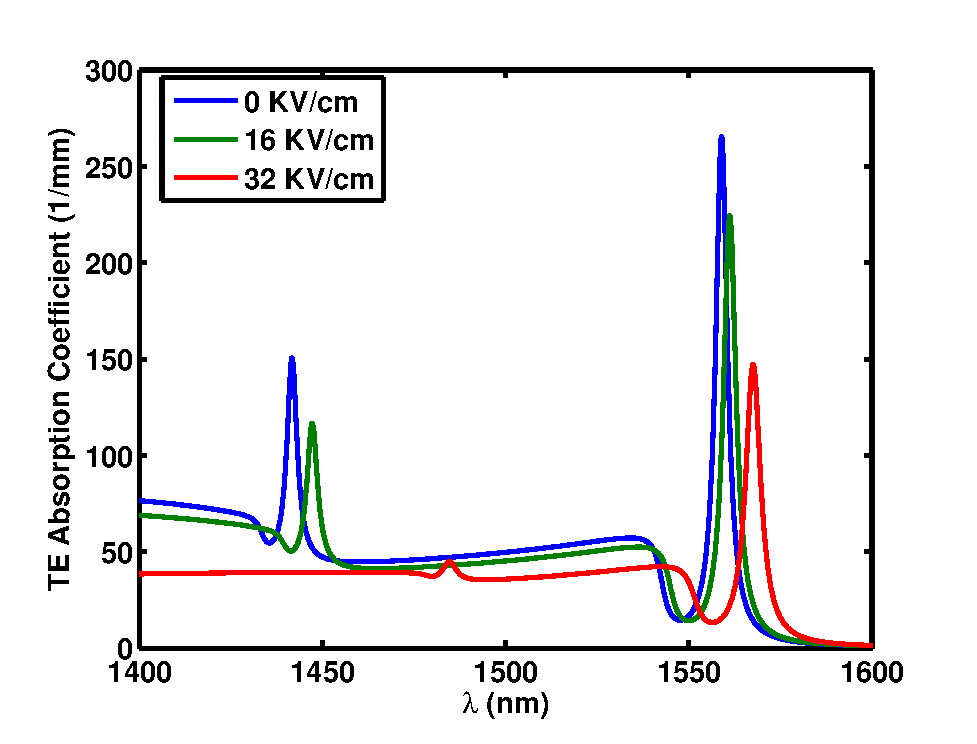
\includegraphics[width=12cm]{./Pictures/fig_ch2_te_abs.eps}
	\caption{TE模式的吸收谱}
	\label{fig_ch2_te_abs}
\end{figure}
\begin{figure}[htb]
	\centering
	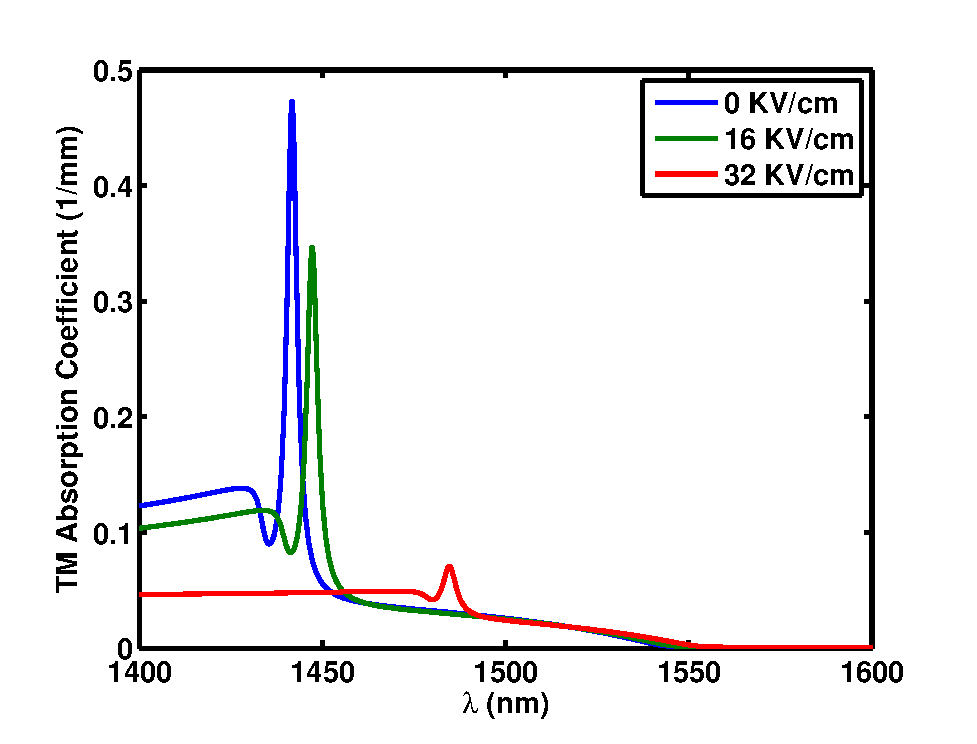
\includegraphics[width=12cm]{./Pictures/fig_ch2_tm_abs.eps}
	\caption{TM模式的吸收谱}
	\label{fig_ch2_tm_abs}
\end{figure}

从图\ref{fig_ch2_te_abs}我们可以看出,量子阱TE偏振吸收谱边沿有强烈的激子吸收峰,并且随着电场的增强往长波移动,其对应的是电子和重空穴跃迁的能量$E_{e-hh}$如图\ref{fig_ch2_ex_abs}(a)所示。而1.45 $\mu m$处对应的小吸收峰是电子和轻空穴跃迁的能量$E_{e-lh}$如图\ref{fig_ch2_ex_abs}(b)。除此之外,激子吸收峰的强度在电场的作用下从$265 mm^{-1}$减弱到$147 mm^{-1}$。从图\ref{fig_ch2_tm_abs}我们可以看出,量子阱TM偏振吸收谱对应的是$E_{e-lh}$,激子吸收峰的强度从$473~ mm^{-1}$减弱到$70~ mm^{-1}$,这是由于轻空穴在强外界电场下从势阱中逃逸,导致轻空穴和电子波函数的叠加积分迅速降低,激子效应减弱。因此,在外界强电场下,高的势垒能,大的空穴与电子等效质量,能保持激子吸收峰的强度,但同时减弱了激子吸收峰随电场的偏移量。这也说明了电吸收调制器中,基于QCSE效应下,在相同长度的材料中,不采用谐振结构时,同时实现高消光比和低驱动电压的光调制器的矛盾。

\subsection{基于退火算法的优化设计}
在设计量子阱时,我们关注的是吸收谱边沿的位置,而设计量子阱的吸收谱边沿是一个多参数优化的问题,吸收谱的位置和量子阱中势阱的宽度$t_w$,以及材料的组分有关。比如我们采用的量子阱是In\SB{x}Al\SB{y}Ga\SB{1-x-y}As材料,势阱和势垒都需要2个参数确定。因此,设计量子阱的吸收谱边沿需要5个参数。在此我们采用了退火算法(Simulated annealing, SA)\cite{Kirkpatrick671}设计量子阱结构。退火算法可用于在受约束条件下寻找多参数的全局最优解。在使用退火算法时,需要注意约束条件的设计和权值函数的设计。合理的约束条件和权值函数能加快退火算法的收敛。

在此利用退火算法,设计了对TE和TM偏振有相同吸收边沿波长位于1530~ nm的量子阱,用于实现偏振不敏感的光调制。本文采用对材料的约束条件是势阱和势垒材料的约束条件相同:0.35 < x < 0.99,0.01 < y < 0.99。量子阱中势阱宽度的约束条件:8 nm < $t_w$ < 15 nm。我们的权值$f_{val}$的表达式如公式\ref{Equ:SAfunvalue}所示。
\begin{equation}
\label{Equ:SAfunvalue}
f_{val} = C_{TE}(\lambda_{TE}-\lambda_{0})^2 + C_{TM}(\lambda_{TM}-\lambda_{0})^2 + C_{diff}(\lambda_{TE}-\lambda_{TM})^2 + C_{w}(t_w-t_{w0})^2,
\end{equation}
其中$C_{TE}, C_{TM}$ 为计算得到的吸收峰边沿$\lambda_{TE}, \lambda_{TM}$与设计值$\lambda_{0}$偏差的权值函数; $C_{diff}$为TE和TM偏振吸收峰之间的距离的权值函数;$C_{w}$为优化得到的量子阱势阱宽度$t_w$和设计值之间的偏差的权值函数;在此我们取:$C_{TE} = C_{TM} = 20; C_{diff} = 100; C_{w} = 10$。由于退火算法是包含随机性,因此每次优化的时间都有所不同。图\ref{fig_ch2_fast_annealing}展示了退火算法的优化过程,可以看到经过了200次迭代,权值函数就已经达到稳定值236。
\begin{figure}[htb]
	\centering
	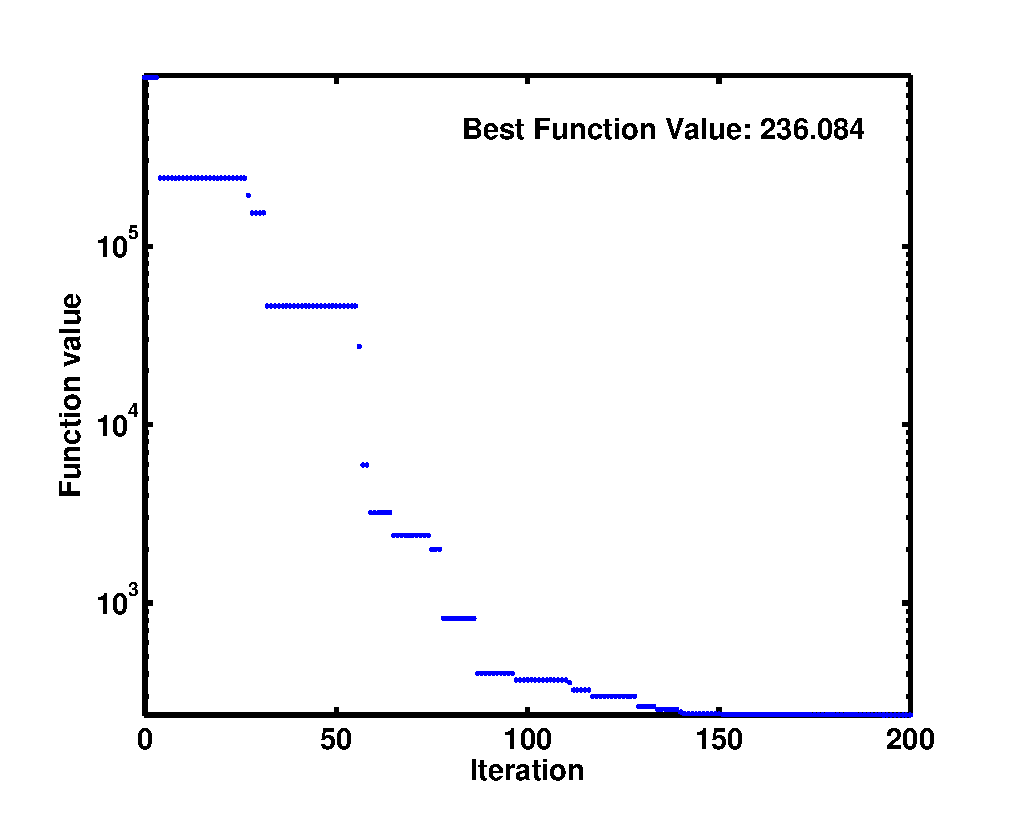
\includegraphics[width=12cm]{./Pictures/fig_ch2_fast_annealing.eps}
	\caption{退火算法的权值函数的优化过程}
	\label{fig_ch2_fast_annealing}
\end{figure}
此时对应量子阱的参数是:势阱$x = 0.495$, $y  = 0.01$;势垒$x = 0.521$,$y = 0.077$;量子阱势阱宽度$t_w = 9.5 nm$。其对应两个偏振吸收峰边沿的波长分别是$ \lambda_{TE} =1529.99~ nm, \lambda_{TM} =  1529.96 ~nm$,两者差值只有0.03nm。在考虑激子效应后,两者波长的分别是$ \lambda_{TE-ex} =1537.58~ nm, \lambda_{TM-ex} =  1538.49~ nm$,两者相差也只有0.91~nm。沿用之前计算吸收谱的参数,此量子阱的吸收谱如图\ref{fig_ch2_opt_abs_tetm},可以看到两个吸收峰位置几乎完全重合,而吸收谱强度的高低主要是由于轻空穴和重空穴波函数的不同,以及$M(E)$见表\ref{METE}和\ref{METM}。
\begin{figure}[htb]
	\centering
	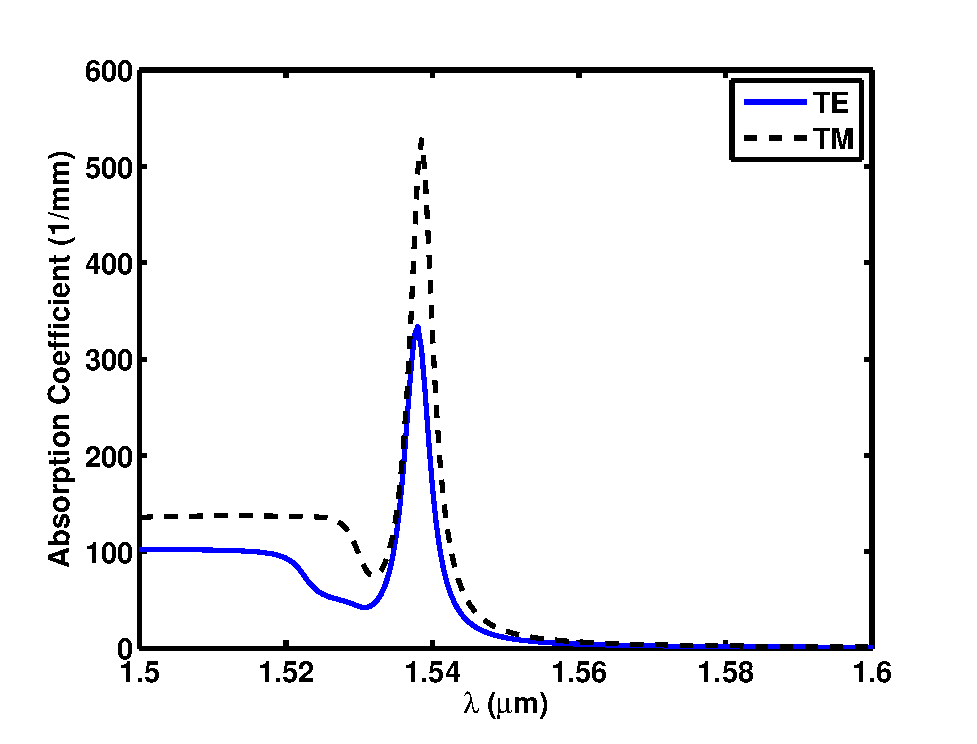
\includegraphics[width=12cm]{./Pictures/fig_ch2_opt_abs_tetm.eps}
	\caption{最后优化的量子阱对TE和TM偏振的吸收谱}
	\label{fig_ch2_opt_abs_tetm}
\end{figure}

\section{III-V外延片的总体设计}
III-V外延结构,不仅包含量子阱的设计,也也包p型重掺杂的欧姆接触层(p contact), 覆盖层(p cladding),隔离限制异质层(Separate Confinement Heterostructure, SCH),n参杂的欧姆接触层(n contact),如图\ref{fig_ch2_banddiagram}(a)所示。其中p contact层为InGaAs,用于和金属电极之间形成欧姆接触,掺杂浓度一般达到1.5$\times$10\SP{19} ~cm\SP{-3}。p cladding层为InP,SCH层是和量子阱相同元素的材料,但是它的折射率比量子阱偏小,能带间隔也偏大以防吸收多量子阱区域的光。SCH层也需要和InP衬底晶格匹配,避免产生额外的应力。p cladding和SCH共同作用使光场约束在多量子阱区域,防止光被重掺杂的p-cladding层和金属电极吸收。通常p pcladding层的厚度达到1.5~$\mu m$。
\begin{figure}[htb]
	\centering
	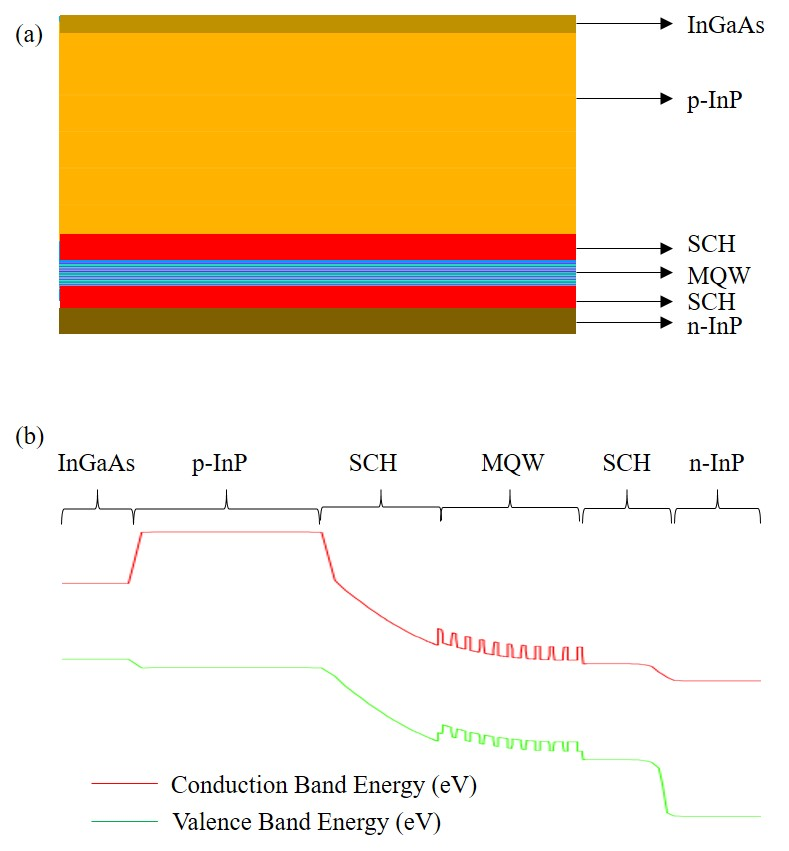
\includegraphics[width=12cm]{./Pictures/fig_ch2_banddiagram.jpg}
	\caption{(a)多量子阱外延片的结构示意图;(b)多量子阱外延片的能带示意图}
	\label{fig_ch2_banddiagram}
\end{figure}

图\ref{fig_ch2_banddiagram}(b)展示了多量子阱的能带示意图,其中量子阱区域能带的弯曲是由于内部p-i-n结的内建电场导致的。多量子阱是由多个量子阱叠加而成的,除了要设计单个单个量子阱的吸收峰外,我们还需要考虑实际工艺中多量子阱中的应力问题。虽然单个量子阱中势阱的应力无法避免,但是通过合理设计势垒的应力以及它的宽度,使总应力$S_{total}$变为0,能增强材料的可靠性\cite{chen2011high}。
\begin{equation}
\label{Equ:strain_net}
S_{total} = t_{w}\epsilon_{w}+t_b\epsilon_b
\end{equation}
其中,$t_{w}$和$t_{b}$分别是多量子阱中势阱和势垒的总厚度,$\epsilon_w$和$\epsilon_b$分别是势阱和势垒的应力。

\section{波导的设计}
在设计用于光调制器的硅基混合集成III-V波导时,我们不仅需要考虑波导在光学上的性能,比如传输损耗,约束因子,等效折射率,群折射率,还需要考虑微波信号传输的特性,比如特征阻抗,微波的等效折射率,传输线的等效电容和电阻。下面将分析矩形波导和蘑菇型波导的两种结构在光学和微波上的性能。这两种波导采用同样的材料参数如表所示\ref{epi_structure}\cite{yongbophd}:
{
	\begin{table}[htb]
		\zihao{5}
		\caption{III-V 波导的材料参数}
		\label{epi_structure}
		\centering
		\begin{tabular}[t]{lllll}
			\hline
			名称 & 厚度 ($\mu m$) & 折射率 n& \tabincell{l}{微波相对 \\ 介电常数 $\epsilon_r$} & 电导率$\delta$ (S/m) \\
			\hline
			p-contact & 0.1 & 3.42 & 13.9 & 20 \\
			p-cladding  & 1.5 & 3.1563 & 12.5 & 1520 \\
			SCH & 0.15 & 3.431 & 13.4 & 0 \\
			MQW & $h_{mqw}$ & 3.491 & 13.5 & 0 \\
			SCH & 0.1 & 3.431 & 13.3 & 32500\\
			n-contact & 0.15 & 3.1563 & 12.5 & 109920 \\
			Metal & 1 & 0.559-$i$9.81 & 1 & 4.1$\times$10\SP{7}\\
			Si & $h_{si}$&3.455 & 11.9 & 10  \\
			SiO2 & 2 & 1.445 & 3.9 & 0\\
			Substrate & >100 & 3.445 & 11.9 & 0.1\\
			BCB & - &1.543 & 2.4336 &0 \\
			\hline
		\end{tabular}
	\end{table}
}
其中,量子阱的厚度$h_{mqw}$和Si波导的厚度$h_{si}$需要后面设计确定。MQW的折射率是利用公式\ref{Equ:nmqw}取得。
\begin{equation}
\label{Equ:nmqw}
n_{mqw}=\sqrt{(t_w n_w^2+t_b n_b^2)/(t_w+t_b)}
\end{equation}
其中,$t_w = ~11 nm, t_b =~ 7 nm, n_w =~ 3.6, n_b = ~3.3$,它们分别是势阱,势垒的宽度和折射率。
\subsection{矩形波导的设计}
早期的纯InP型波导型电吸收光调制器都是采用矩形波导\cite{zhang1999traveling,Robertphd,yuphd}。虽然矩形波导的光调制器相比与蘑菇型波导的光调制器具有工艺简单的特点\cite{chiu2005enhanced},但是由于传统的矩形波导的光的群速度和微波的传播速度失配,微波的特种阻抗无法达到微波标准阻抗$50 ~\Omega$,相对蘑菇型波导有比较大的结电容,因此这三项限制了矩形波导在光调制器中的应用。而在硅基混合平台上实现的光调制器至今都是采用蘑菇型波导\cite{kuo2008high, tang201150, tang2012over, tang2012energy, chen2011forty},在此我们将首次分析硅基混合平台上矩形波导作为光调制器的特点。
\begin{figure}[htb]
	\centering
	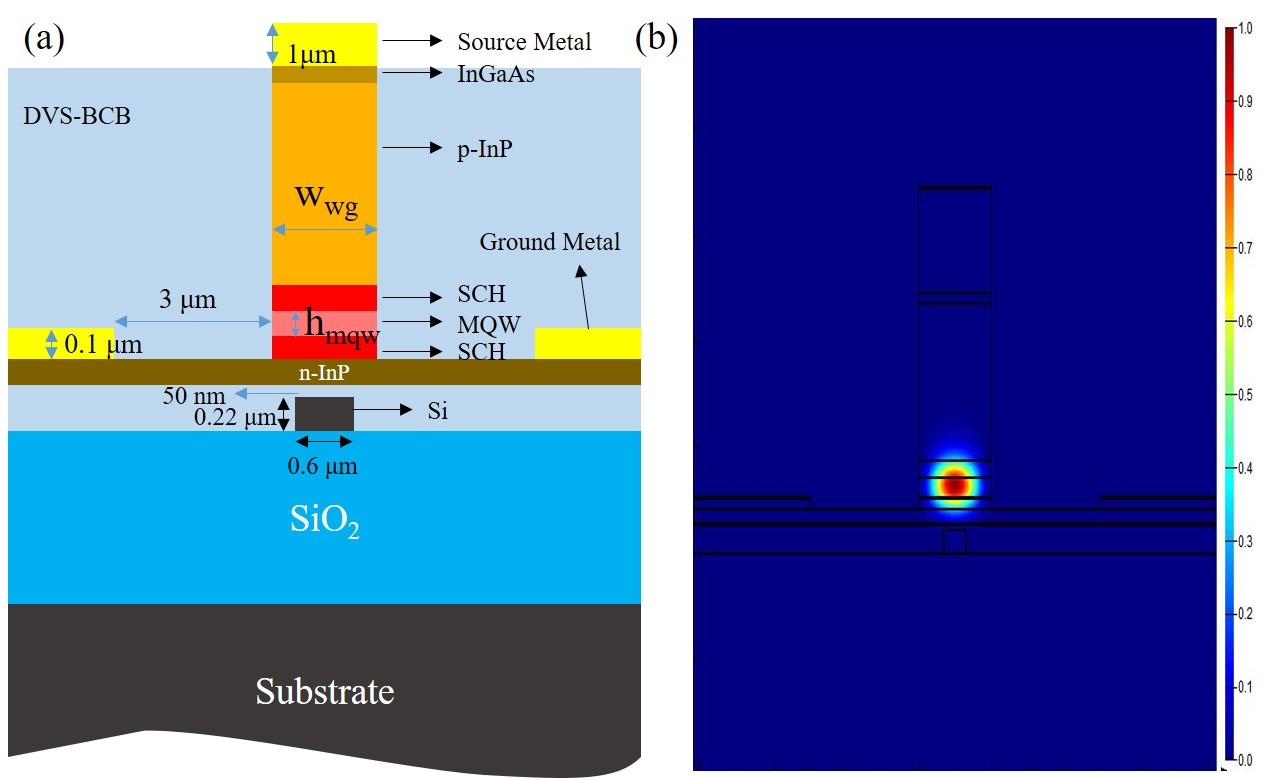
\includegraphics[width=12cm]{./Pictures/fig_ch2_rect_structure_mode.jpg}
	\caption{(a) 矩形波导截面示意图;(b) 矩形波导模场分布图,其中$w_{wg} = 2~ \mu m, h_{mqw} = 0.15 ~\mu m, \lambda_0 = 1.55\mu m$}
	\label{fig_ch2_rect_structure_mode}
\end{figure}

矩形波导的截面图如图\ref{fig_ch2_rect_structure_mode}(a)所示。其有很多参数需要设计,比如波导的宽度$w_{wg}$,多量子的厚度$h_{mqw}$,金属电极的厚度,地电极和波导之间的距离。在此,我们首先考虑波导宽度和多量子阱厚度对波导光学性能上的影响。而金属电极的厚度和地电极和波导之间的距离虽然在光学上只会影响波导损耗,但是对微波上的影响更为明显。在光学性能分析中,金属电极的设计参数如图\ref{fig_ch2_rect_structure_mode}(a)所示。图\ref{fig_ch2_rect_structure_mode}(b)展示了当$w_{wg} = 2 ~\mu m, h_{mqw} = 0.15 ~\mu m$, 工作波长$\lambda_0 = 1.55~\mu m$时的模场分布。可以看到大部分光场集中在多量子阱区域。


下面分析当矩形波导的宽度从$0.8 ~\mu m$变化到$3 \mu m$, 量子阱的高度从 $0.05 ~\mu m$变化到$0.2 ~\mu m$时,波导的等效折射率$n_{eff}$,群折射率$n_g$,损耗$loss$和光强在量子阱所占的百分比,即约束因子(confinement factor),的变化。我们采用Lumerical公司的MODE Solution进行计算\cite{modesolution},结果如图所示\ref{fig_ch2_rect_property}。

\begin{figure}[htb]
\small
\subfigure[]{
	\begin{minipage}[]{0.5\textwidth}
		\centering
		\label{fig_ch2_rect_neff}
		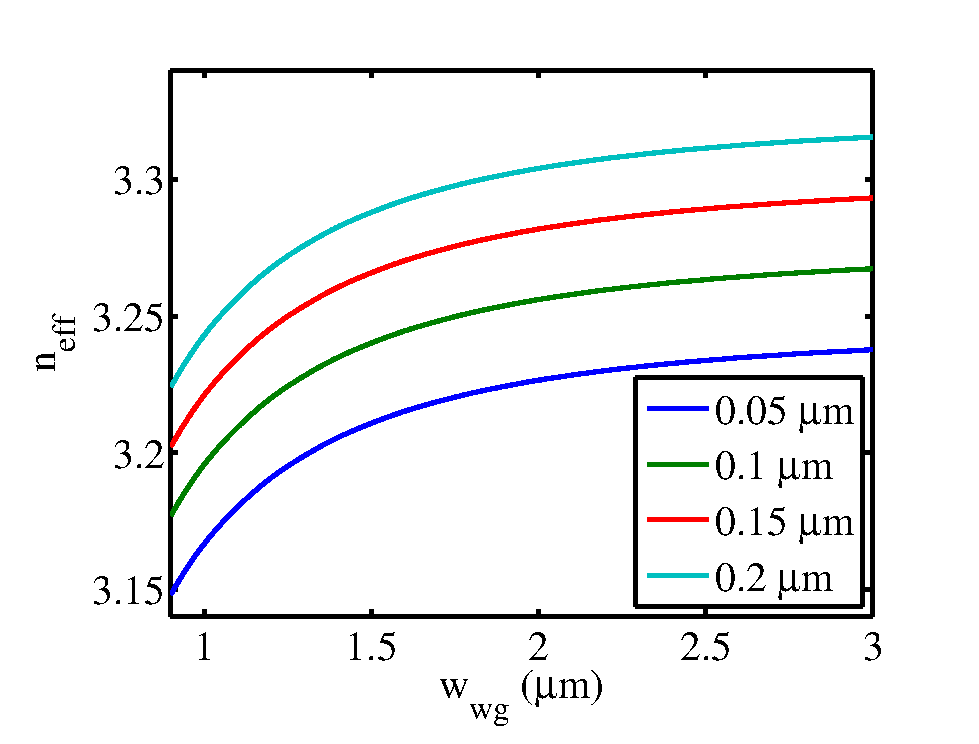
\includegraphics[width=8cm]{./Pictures/fig_ch2_rect_neff.eps}
	\end{minipage}}
\subfigure[]{
	\begin{minipage}[]{0.5\textwidth}
		\centering
		\label{fig_ch2_rect_ng} %% label for second subfigure
		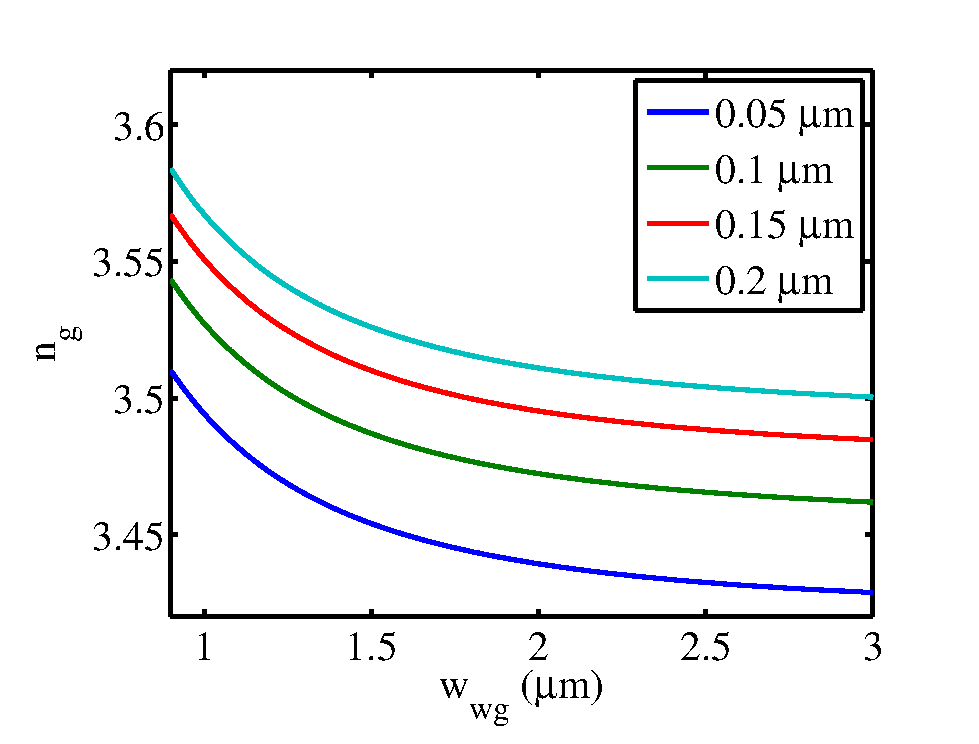
\includegraphics[width=8cm]{./Pictures/fig_ch2_rect_ng.eps}
	\end{minipage}}
\subfigure[]{
	\begin{minipage}[]{0.5\textwidth}
		\centering
		\label{fig_ch2_rect_loss} %% label for second subfigure
		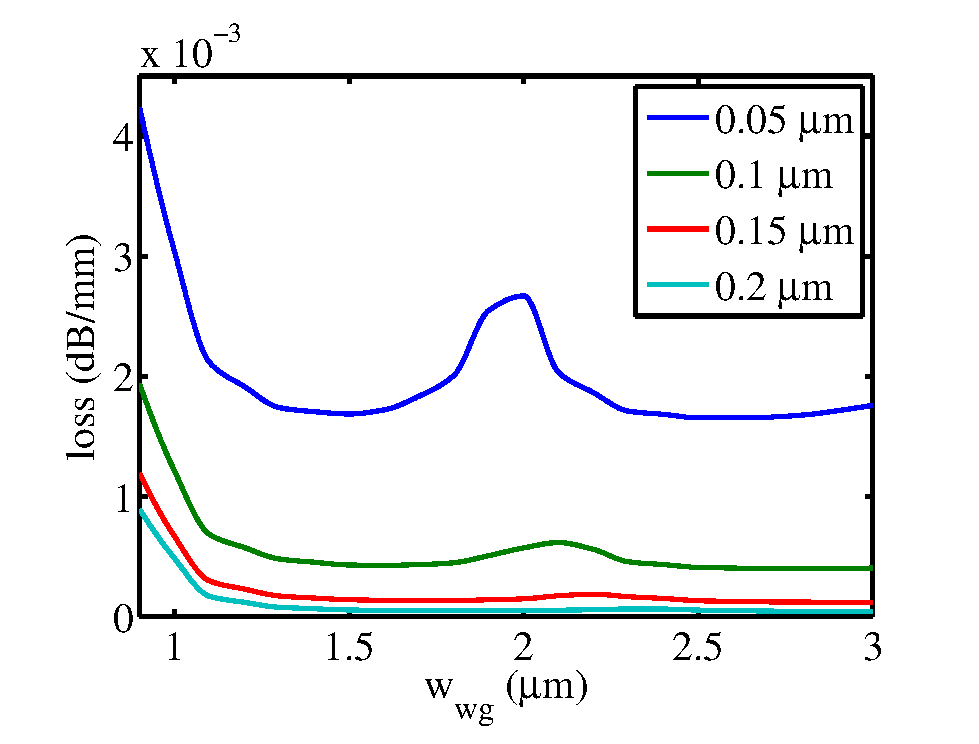
\includegraphics[width=8cm]{./Pictures/fig_ch2_rect_loss.eps}
	\end{minipage}}
\subfigure[]{
	\begin{minipage}[]{0.5\textwidth}
		\centering
		\label{fig_ch2_rect_confinement} %% label for second subfigure
		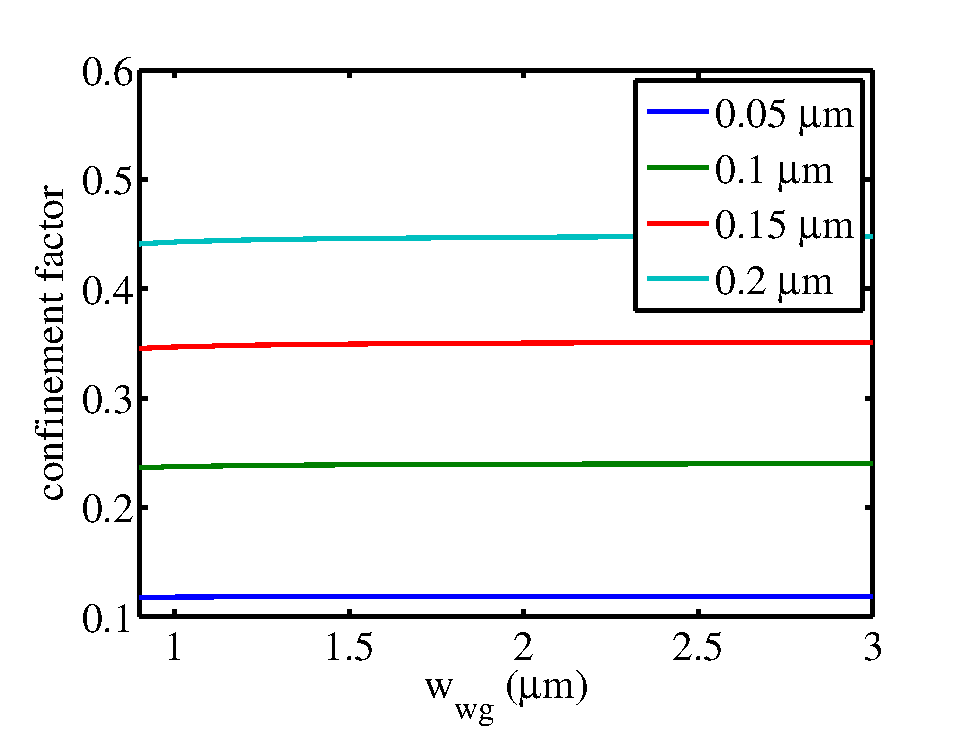
\includegraphics[width=8cm]{./Pictures/fig_ch2_rect_confinement.eps}
	\end{minipage}}
\caption{图(a)-(d)分别是在不同量子阱厚度下,矩形波导的$n_{neff}, n_g, loss, confinement~factor$随$w_{wg}$的关系,工作波长$\lambda_0 = ~1.55\mu m$}
\label{fig_ch2_rect_property}
\end{figure}

从图\ref{fig_ch2_rect_neff}可以看到,随着矩形波导的宽度和量子阱厚度的增加,等效折射率都在递增。而随着宽度的增加,等效折射率趋于稳定,但是随着高度的增加等效折射率线性增加。不过,高度继续增加的话,等效折射率也会逐渐趋向于量子阱材料的折射率。

等效折射率表征了光相位的变化速度,而调制器光信号的传输速度则与群折射率有关。从图\ref{fig_ch2_rect_ng}可以看到,随着波导宽度的增加,群折射率逐渐减小,而量子阱厚度增加群折射率反而提高。

波导的损耗可以从图\ref{fig_ch2_rect_loss}看出,随着波导宽度和量子阱高度的增加,越来越多的光约束在量子阱区域,因此损耗也会降低。可以看到当量子阱厚度大于$0.15~ \mu m$,波导宽度大于$1~ \mu m$时,损耗对波导尺寸的变化不敏感。

从图\ref{fig_ch2_rect_confinement}可以看到量子阱的厚度逐渐增加约束因子逐渐提高,约束因子对波导的宽度不敏感。当波导宽度从$1 ~\mu m$变化到$3 ~\mu m$,约束因子只有不到1\%的提高。

下面我们将分析矩形波导的微波特性。我们采用Ansys公司的HFSS进行计算\cite{ansyshfss}。图\ref{fig_ch2_rect_microwave_mode_equal_circuits}(a)展示了当$w_{wg} =~2 \mu m, h_{mqw} =~ 0.15 \mu m$,微波频率$f_m =~ 40 GHz$时的微波模场的分布。相比图\ref{fig_ch2_rect_structure_mode}(a)所示的光场分布图,微波分布图大部分能量也是集中于MQW和SCH本征层中,但是由于微波波长远大于通信波段的波长,因此微波更多的能量泄漏到量子阱外面。
\begin{figure}[htb]
	\centering
	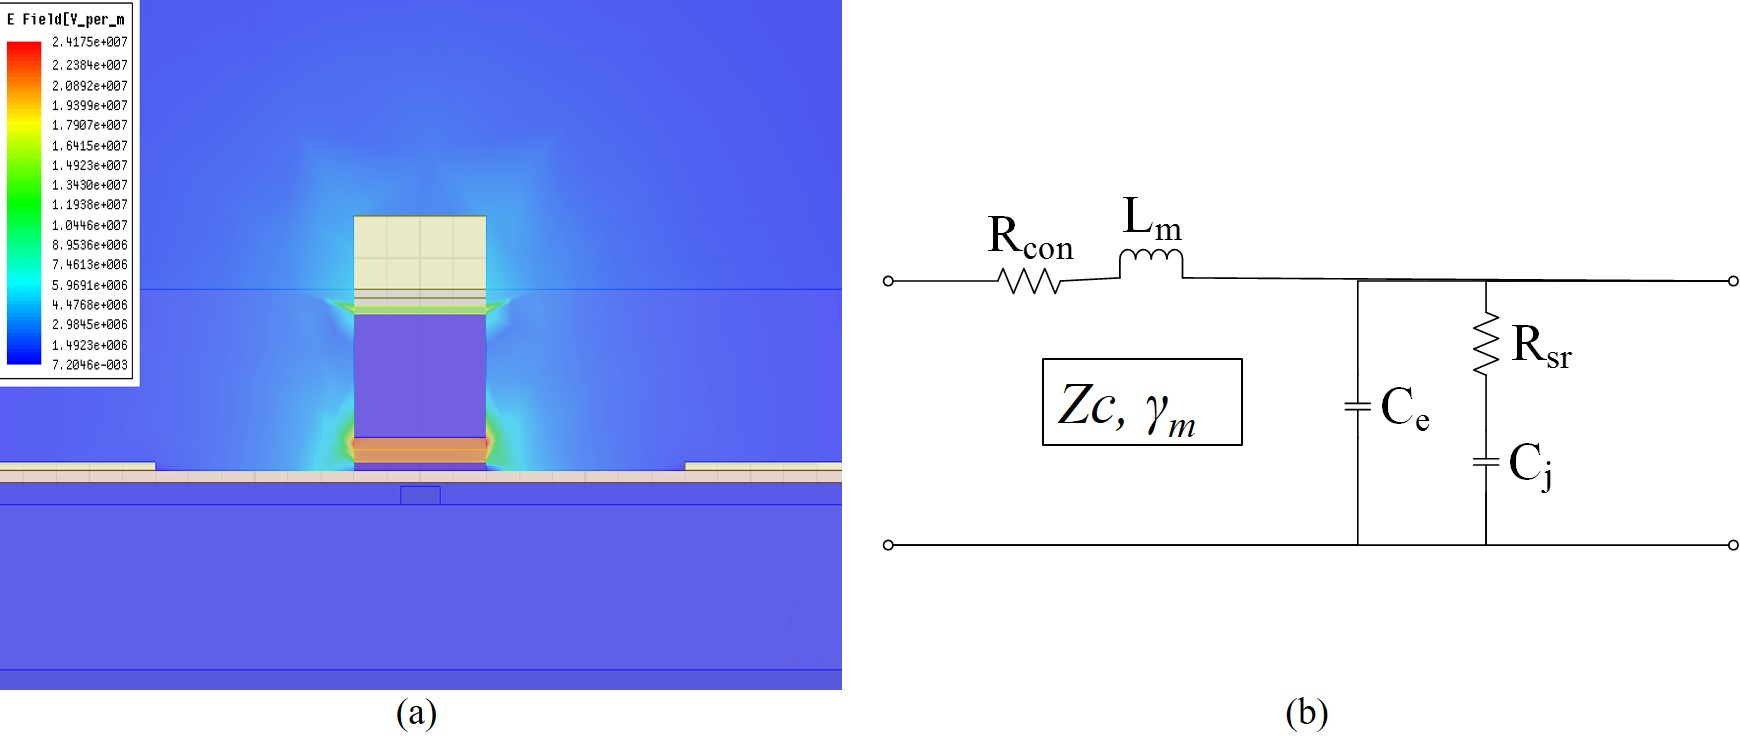
\includegraphics[width=12cm]{./Pictures/fig_ch2_rect_microwave_mode_equal_circuits.jpg}
	\caption{(a) 矩形波导微波$f_m = 40~GHz$的模式分布,其中$w_{wg} = 2~\mu m, h_{mqw} = 0.15~\mu m$;(b) 微波小信号等效电路模型}
	\label{fig_ch2_rect_microwave_mode_equal_circuits}
\end{figure}

由于矩形波导微波上对应的结构属于微带线(microstrip  line)结构,色散比较小,群折射率和等效折射率相同。描述微波的模式除了用等效折射率$n_m$外,还需要用本征阻抗(Characteristic Impedance,$Z_C$)来描述电学性能。我们可以采用微波小信号等效电路用金属电阻$R_{con}$,串联电阻$R_{sr}$,结电容$C_j$,寄生电容$C_e$,金属电感$L_m$,来表述$n_m, Z_C$。
\begin{equation}
\label{Equ:zc}
Z_C(\omega) = \sqrt{\frac{Z_S(\omega)}{Y_p(\omega)}}
\end{equation}
\begin{equation}
\label{Equ:gammam}
\gamma_m(\omega) = jn_m(\omega)\frac{\omega}{c_0} + \alpha_m(\omega) = \sqrt{Z_S(\omega)Y_p(\omega)}
\end{equation}
其中
\begin{equation}
\label{Equ:zs}
Z_S(\omega) = R_{con}+j\omega L_m
\end{equation}
\begin{equation}
\label{Equ:yp}
Y_p(\omega) = \frac{j\omega C_j}{1+j\omega C_jR_{sr}}+j\omega C_e
\end{equation}
根据文献[\citenum{li1999ultrahigh}]近似可得:
\begin{equation}
\label{Equ:zcsimple}
Z_C = \sqrt{\frac{L_m}{C_j+C_e}}
\end{equation}
\begin{equation}
\label{Equ:nmsimple}
n_m = \frac{c_0}{\omega}\left(\frac{R_{con}}{2Z_C} + \frac{\omega^2}{2}C^2_jR_{sr}Z_C\right)
\end{equation}
\begin{equation}
\label{Equ:alphasimple}
\alpha_m = \omega\sqrt{L_m(C_j+C_e)}
\end{equation}
从公式\ref{Equ:zcsimple}和\ref{Equ:alphasimple}可以看出,通过减小电容,我们能够同时增大特征阻抗和减小微波损耗。从图\ref{fig_ch2_rect_microwave_mode_equal_circuits}(a)可以看出本征层MQW和SCH是结电容器,微波的大部分能量集中于此。因此,通过增加本征层的厚度或者波导的宽度可以减小电容,提高阻抗。但是增加本征层的厚度,同时增加了所需的调制器电压。另外考虑到当量子阱的厚度小于$0.1 ~\mu m$时,光学损耗明显增加,如图\ref{fig_ch2_rect_loss}。因此我们只分析当量子阱厚度为为$0.15~ \mu m$和$0.2 ~\mu m$时的特性。
\begin{figure}[htb]
	\small
	\subfigure[]{
		\begin{minipage}[]{0.5\textwidth}
			\centering
			\label{fig_ch2_rect_zc}
			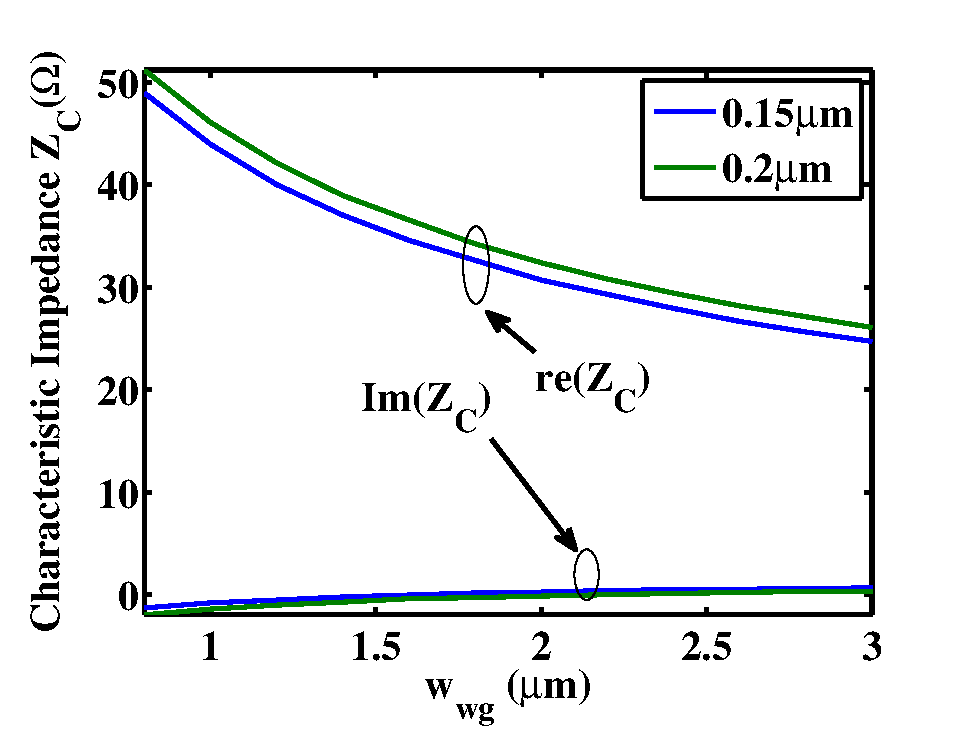
\includegraphics[width=8cm]{./Pictures/fig_ch2_rect_zc.eps}
		\end{minipage}}
	\subfigure[]{
		\begin{minipage}[]{0.5\textwidth}
			\centering
			\label{fig_ch2_rect_neff_ng} %% label for second subfigure
			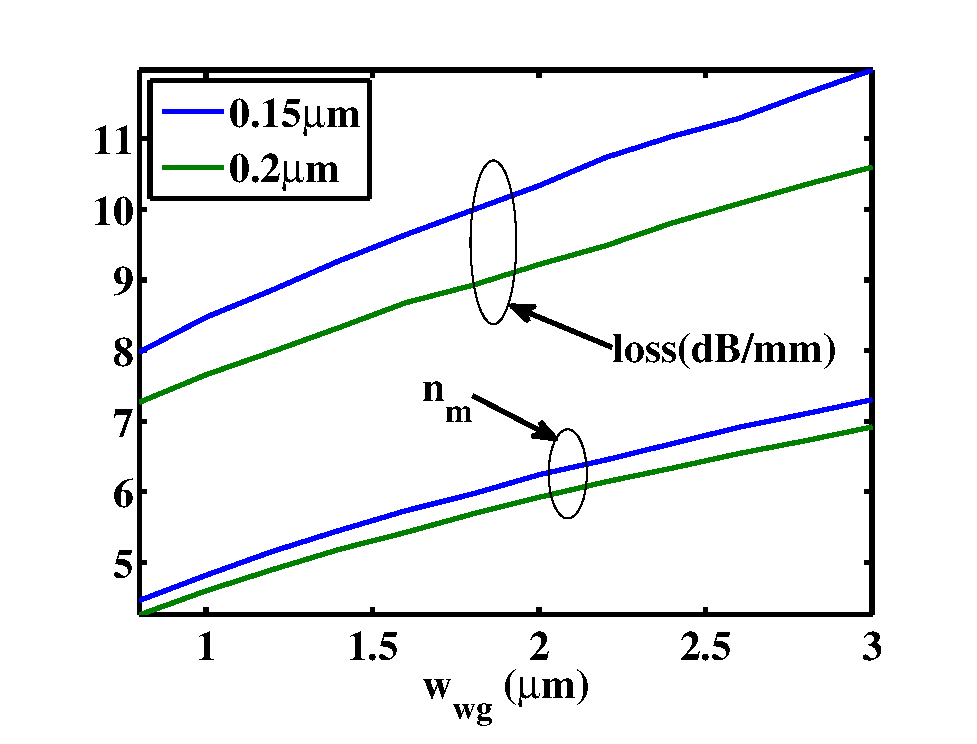
\includegraphics[width=8cm]{./Pictures/fig_ch2_rect_neff_ng.eps}
	\end{minipage}}
\caption{(a), (b)分别是$f_m = 40~GHz$时,在不同量子阱厚度下,矩形波导微波的本征阻抗$Z_C$,微波损耗$loss$,微波等效折射率$n_m$随$w_{wg}$的关系}
\label{fig_ch2_rect_microwave_property}	
\end{figure}
从图\ref{fig_ch2_rect_zc}可以看出,当波导宽度逐渐减小时或者量子阱厚度逐渐增大,导致结电容减小,因而本征阻抗逐渐提高。当$w_{wg} = 0.8~ \mu m$时,特征阻抗达到50~ $\Omega$。并且,量子阱厚度从0.15~$\mu m$增加到$0.2~\mu m$,本征阻抗变化量小。从图\ref{fig_ch2_rect_neff_ng}可以看出,微波损耗和微波的等效折射率随着同样也随着结电容的减小而减小。本征阻抗,微波损耗,微波等效折射率的变化与公式\ref{Equ:zcsimple},\ref{Equ:nmsimple},\ref{Equ:alphasimple}描述一致。

完美的行波电极调制器,需要满足微波的和光波群速度匹配,微波电阻和$50~\Omega$匹配。而目前,文献[\citenum{tang201150, zhang1999traveling}]中所展示的利用行波电极的电吸收光调制器,都没有达到这两点。之前的研究人员,通常采用分段式传输线电极,通过高阻抗高群速度和低阻抗低群速度的两种微波电极结构在小于微波波长尺寸内相互组合,达到阻抗匹配,相速度近似匹配的条件,以实现高的调制速度\cite{tang2012over,yuphd,Robertphd}。不过,分段传输线的电极结构尺寸大于行波电极结构。而在硅基混合集成平台上通过减小波导的宽度,以及合适量子阱高度,就能实现标准50~ $\Omega$完美匹配。之所以,在之前的InP基电吸收吸收光调制器中无法通过这种方式实现完美的阻抗匹配,是因为InP基的电吸收光调制器的纵向光约束能力太弱,无法实现宽度小于1~$\mu m$低损耗的波导。

借助于硅基混合集成平台能实现窄波导的特点,我们下面我们分析这种结构的调制器用行波电极的电光调制带宽。我们采用的量子阱高度是$0.187~ \mu m$与文献[\citenum{tang201150}]保持一致。当波导宽度$w_{wg} = 0.8~ \mu m$时,光学$1.55~ \mu m$的$n_g = 3.6, loss = 1.9 \times 10^{-3} ~dB/cm^{-1} $,而微波的本征阻抗$Z_C$,微波损耗$loss$,微波等效折射率$n_m$随工作频率$f$的关系如图\ref{fig_ch2_rect_freq_property}所示。
\begin{figure}[htb]
	\small
	\subfigure[]{
		\begin{minipage}[]{0.5\textwidth}
			\centering
			\label{fig_ch2_rect_freq_zc}
			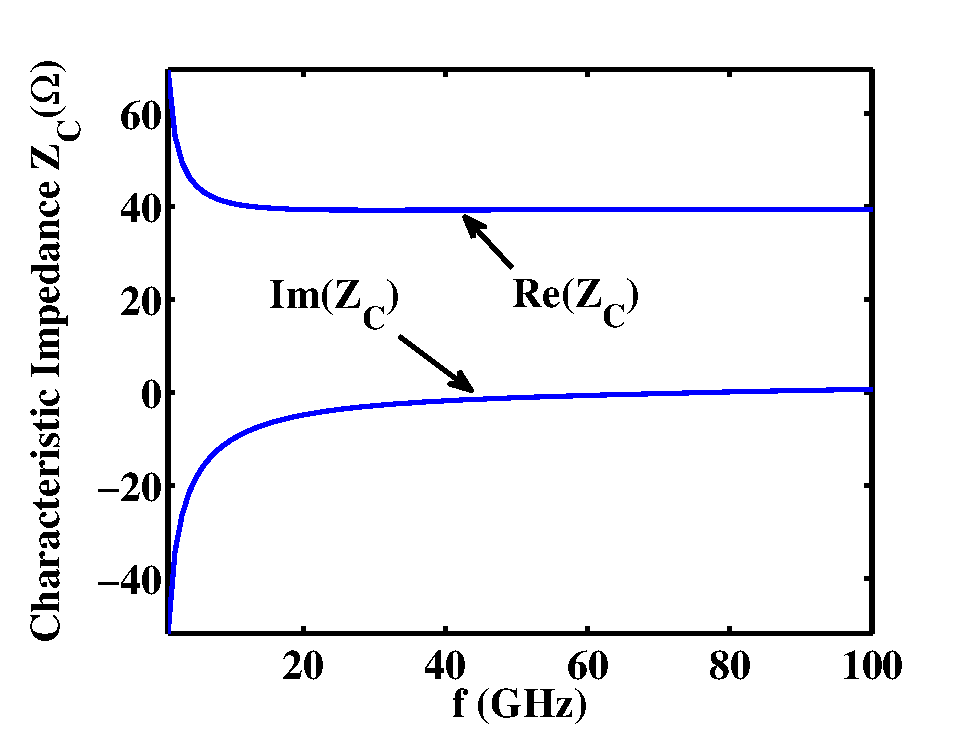
\includegraphics[width=8cm]{./Pictures/fig_ch2_rect_freq_zc.eps}
	\end{minipage}}
	\subfigure[]{
		\begin{minipage}[]{0.5\textwidth}
			\centering
			\label{fig_ch2_rect_freq_neff_loss} %% label for second subfigure
			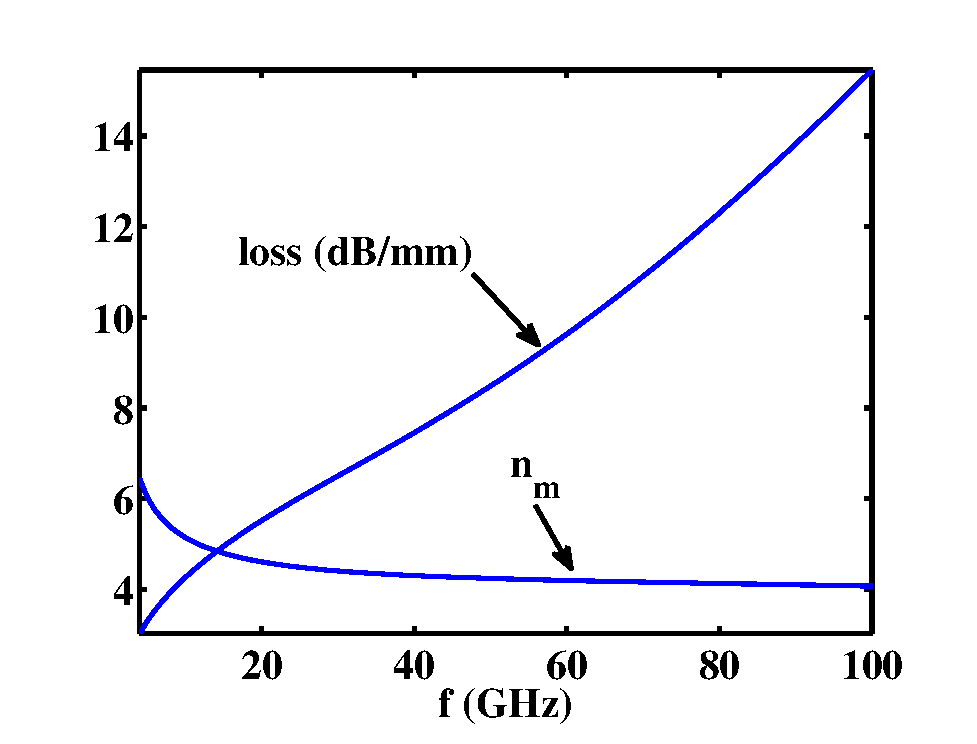
\includegraphics[width=8cm]{./Pictures/fig_ch2_rect_freq_neff_loss.eps}
		\end{minipage}}
\caption{(a), (b)分别是$w_{wg} = 0.8 ~\mu m, h_{mqw} = 0.187 ~\mu m$时,在不同量子阱厚度下,矩形波导微波的本征阻抗$Z_C$,微波损耗$loss$,微波等效折射率$n_m$随频率$f$的关系}
\label{fig_ch2_rect_freq_property}	
\end{figure}

根据波导在光学和微波的特性,计算电吸收调制器的调制带宽如下式\cite{li1999ultrahigh, tang2008design}:
\begin{equation}
\label{Equ:eoresponse}
R_{EO} = \left|\frac{1}{1+j\omega R_{rs} C_j}\frac{T}{1-\Gamma_L \Gamma_S  e^{-2 \gamma_m L} } \left\{\frac{e^{(j\beta_o-\gamma_m)L}-1}{(j\beta_o-\gamma_m)L}+\Gamma_L e^{-2\gamma_m L} \frac{e^{(j\beta_o+\gamma_m)L}-1}{(j\beta_o+\gamma_m)L} \right\} \right|^2,
\end{equation}
其中,$\beta_o = 2n_g\pi/\lambda_0, \lambda_0 = 1.55~\mu m $;微波反射系数$\Gamma_S=(Z_S-Z_C)/(Z_S+Z_C)$;$\Gamma_L=(Z_L-Z_C)/(Z_L+Z_C)$,$Z_S, Z_L$是源和负载的特征阻抗,在此我们取标准的$50~ \Omega$;调制器长度$L = 100~ \mu m$;依据文献[\citenum{tang2012over}],我们取$R_{rs} C_j=1.3~ ps$。图\ref{fig_ch2_rect_3dB_S11}展示了电光响应$R_{EO}$的带宽和微波的反射系数$S_{11}$的幅值。从图\ref{fig_ch2_rect_3dB}可以看到$R_{EO}$的3~dB带宽$f_{3dB}\approx ~100 GHz$,并且图\ref{fig_ch2_rect_S11}展示了微波的反射系数在0~GHz到100~GHz的范围内都低于-25~dB。而目前最好的硅基混合集成光调制器,利用分段传输线式电极,其3~dB带宽达到74~GHz,反射系数在高频也无法保持在-20~dB以下\cite{tang2012over}。
\begin{figure}[htb]
	\small
	\subfigure[]{
		\begin{minipage}[]{0.5\textwidth}
			\centering
			\label{fig_ch2_rect_3dB}
			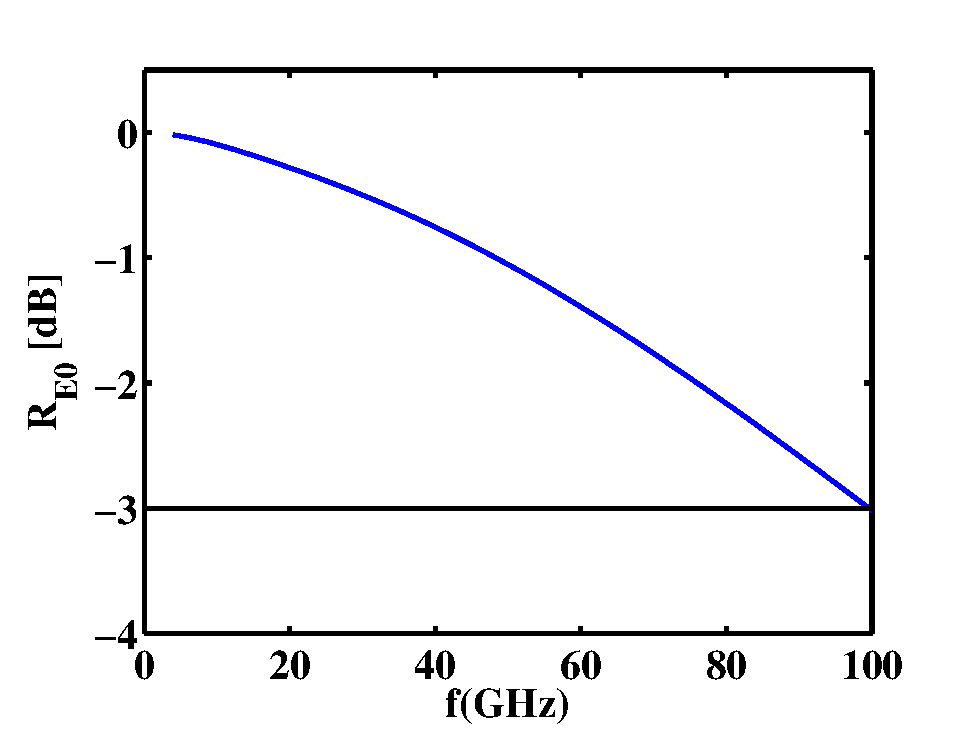
\includegraphics[width=8cm]{./Pictures/fig_ch2_rect_3dB.eps}
		\end{minipage}}
	\subfigure[]{
		\begin{minipage}[]{0.5\textwidth}
			\centering
			\label{fig_ch2_rect_S11} %% label for second subfigure
			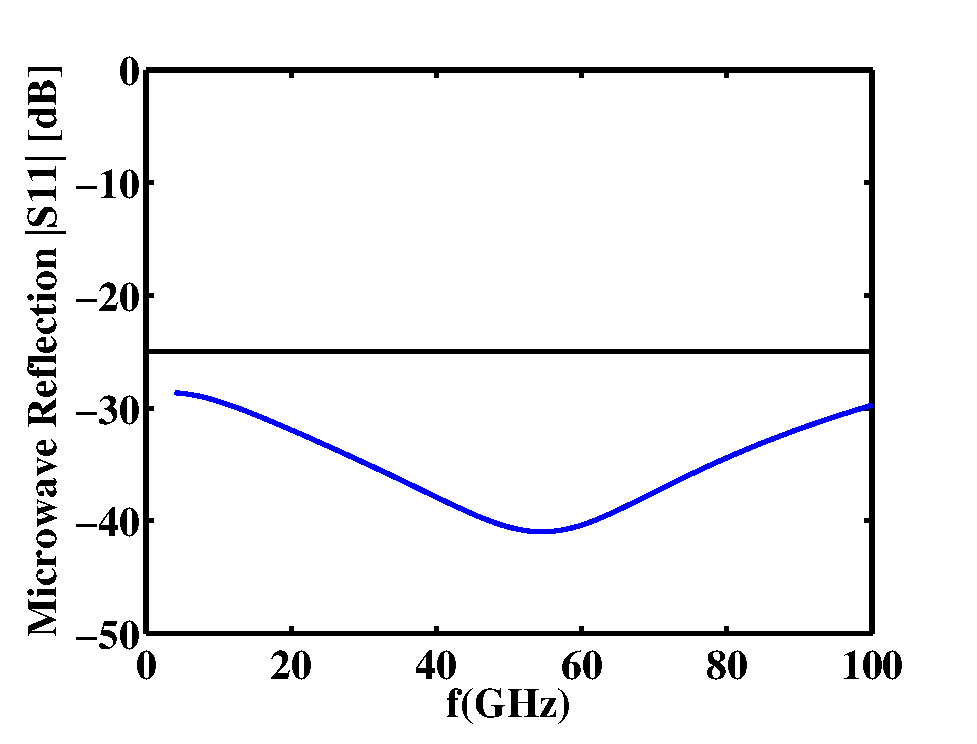
\includegraphics[width=8cm]{./Pictures/fig_ch2_rect_S11.eps}
		\end{minipage}}
\caption{(a)矩形波导调制器的电光调制器带宽$R_{EO}$;(b)矩形波导调制器的微波反射系数$|S_{11}|$}
\label{fig_ch2_rect_3dB_S11}	
\end{figure}
		
\subsection{蘑菇型波导的设计}
蘑菇型波导是利用MQW和SCH材料与InP有选择性腐蚀的特点,实现MQW和SCH区域的宽度小于p-InP层的宽度,从而降低波导的结电容$C_j$。蘑菇型波导可以先定义宽的波导掩膜,或者直接用比较宽的p-InP作为掩膜,再利用选择性腐蚀液,将量子阱区域内掏(undercut)变窄,从而降低了光刻精度,可用接触式光刻制作,因此被广泛用于电吸收光调制器\cite{chiu2005enhanced, kuo2008high, tang201150, tang2012over, tang2012energy, chen2011forty}。

蘑菇型波导的截面图如图\ref{fig_ch2_ms_structure_mode}(a)所示。相比矩形波导,蘑菇型波导的宽度有更多的待定参数,在此我们限定p-InP的宽度为2.5$\mu m$,这个尺寸是可以用接触式光刻达到。而蘑菇型波导的宽度$w_{wg}$,我们定义为多量子阱区域的宽度。其他的结构参数的定义和矩形波导保持一制,见图\ref{fig_ch2_ms_structure_mode}(a)。我们首先考虑$w_{wg}$和$h_{mqw}$对波导光学性能上的影响。图\ref{fig_ch2_ms_structure_mode}(b)展示了当$w_{wg} = 2 ~\mu m, h_{mqw} = 0.15 ~\mu m$, 工作波长$\lambda_0 = 1.55~\mu m$时的模场分布。可以看到大部分光场集中在多量子阱区域。不过相比矩形波导的模式\ref{fig_ch2_rect_structure_mode}(b),蘑菇型波导中有部分光约束在硅波导中。
\begin{figure}[htb]
	\centering
	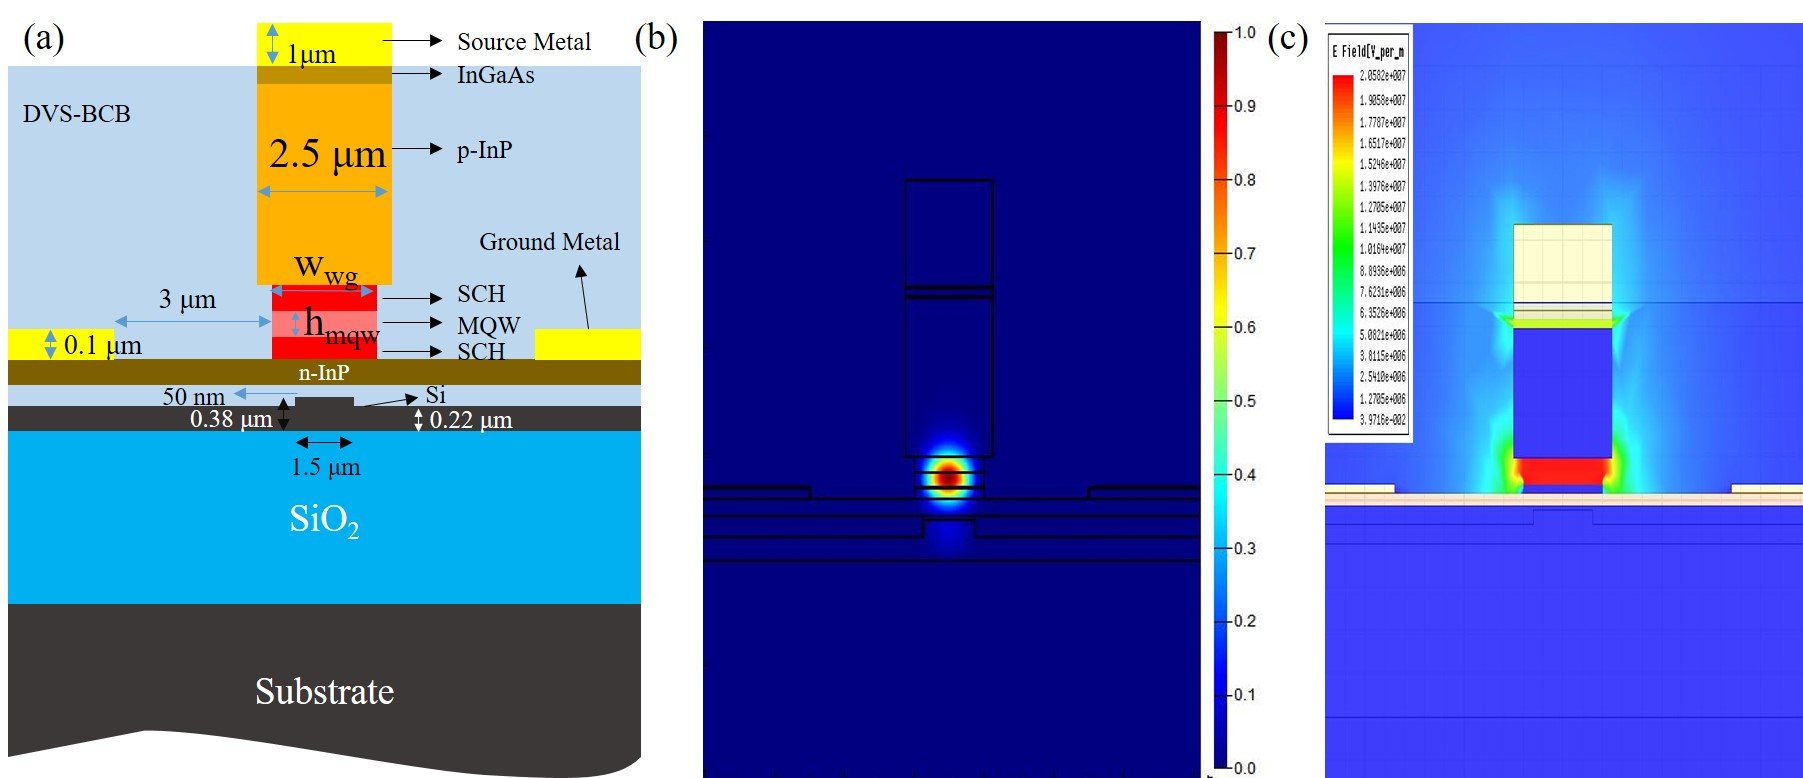
\includegraphics[width=16cm]{./Pictures/fig_ch2_ms_structure_mode.jpg}
	\caption{(a) 蘑菇型波导截面示意图;(b) 蘑菇型波导模场分布图,其中$w_{wg} = 2~ \mu m, h_{mqw} = 0.15 ~\mu m, \lambda_0 = 1.55~\mu m$;(c) 蘑菇型波导微波$f_m = 40~GHz$的模式分布,其中$w_{wg} = 2~\mu m, h_{mqw} = 0.15~\mu m$}
	\label{fig_ch2_ms_structure_mode}
\end{figure}

下面分析当蘑菇型波导的宽度从$0.8 ~\mu m$变化到$3 \mu m$, 量子阱的高度从 $0.05 ~\mu m$变化到$0.2 ~\mu m$时,蘑菇型波导的等效折射率$n_{eff}$,群折射率$n_g$,损耗$loss$和光强在量子阱所占的百分比,即约束因子(confinement factor),的变化。我们采用Lumerical公司的MODE Solution进行计算\cite{modesolution},结果如图所示\ref{fig_ch2_ms_property}。

\begin{figure}[htb]
	\small
	\subfigure[]{
		\begin{minipage}[]{0.5\textwidth}
			\centering
			\label{fig_ch2_ms_neff}
			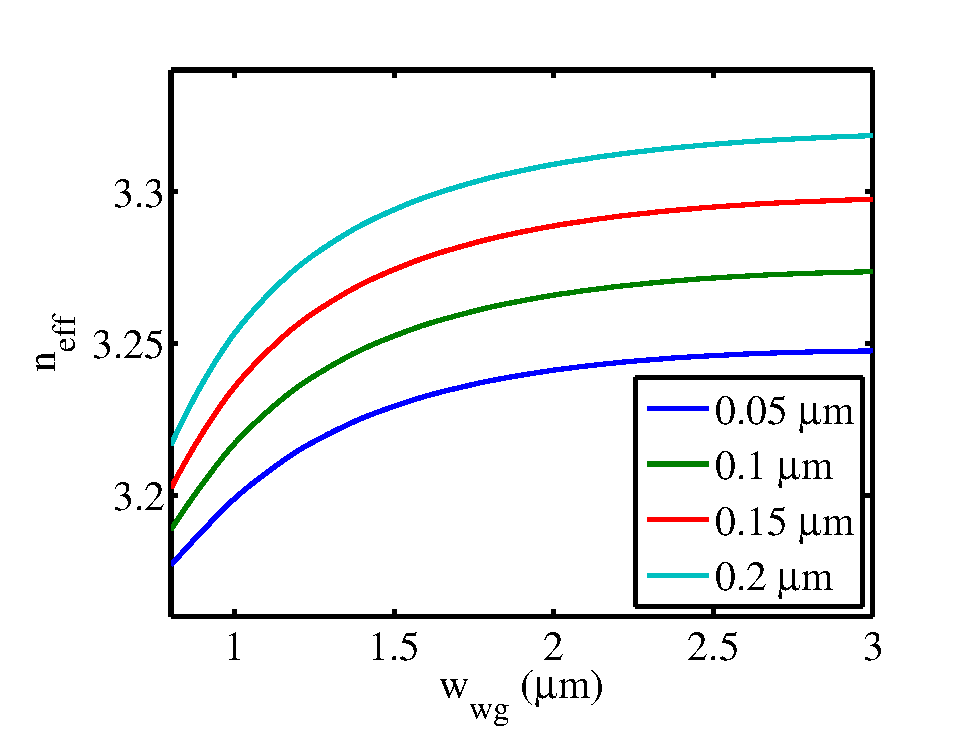
\includegraphics[width=8cm]{./Pictures/fig_ch2_ms_neff.eps}
		\end{minipage}}
	\subfigure[]{
		\begin{minipage}[]{0.5\textwidth}
			\centering
			\label{fig_ch2_ms_ng} %% label for second subfigure
			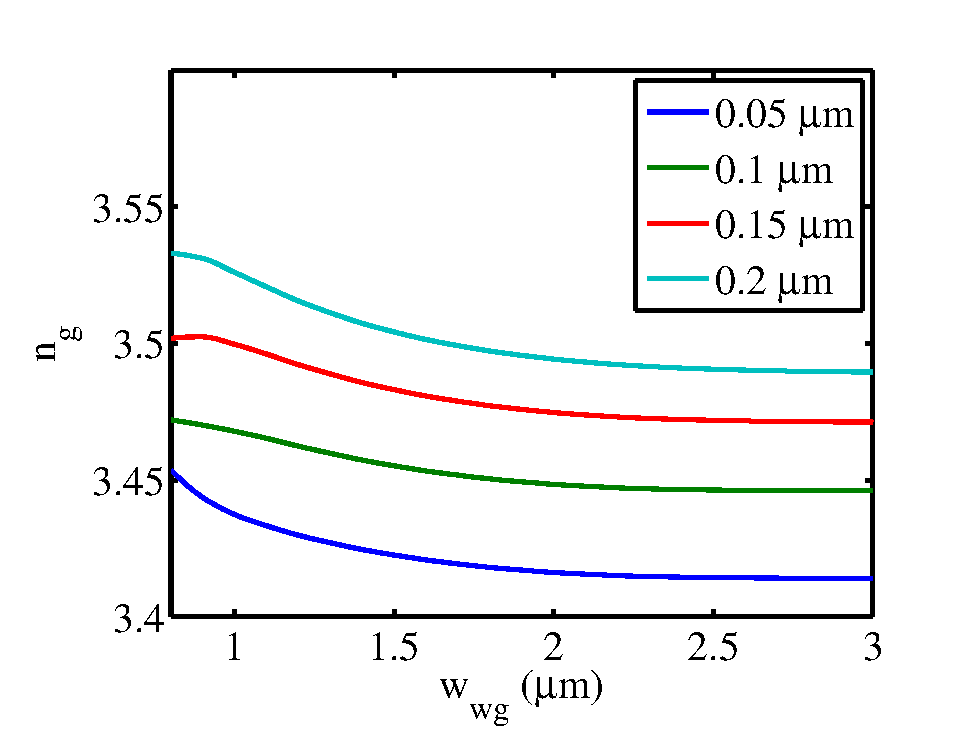
\includegraphics[width=8cm]{./Pictures/fig_ch2_ms_ng.eps}
		\end{minipage}}
	\subfigure[]{
		\begin{minipage}[]{0.5\textwidth}
			\centering
			\label{fig_ch2_ms_loss} %% label for second subfigure
			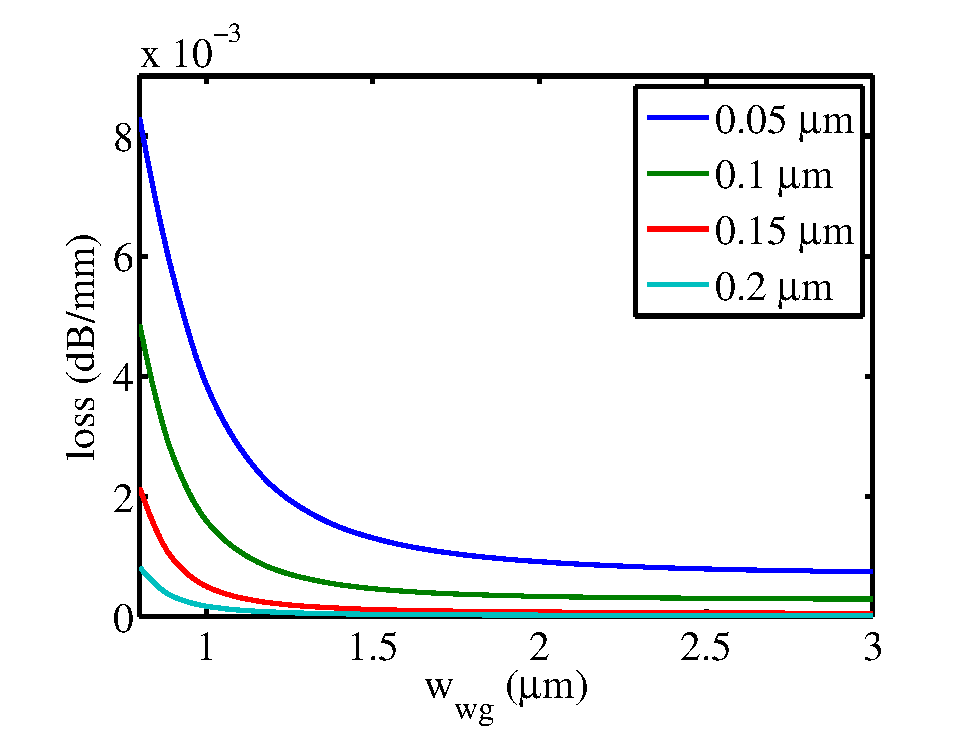
\includegraphics[width=8cm]{./Pictures/fig_ch2_ms_loss.eps}
		\end{minipage}}
	\subfigure[]{
		\begin{minipage}[]{0.5\textwidth}
			\centering
			\label{fig_ch2_ms_confinement} %% label for second subfigure
			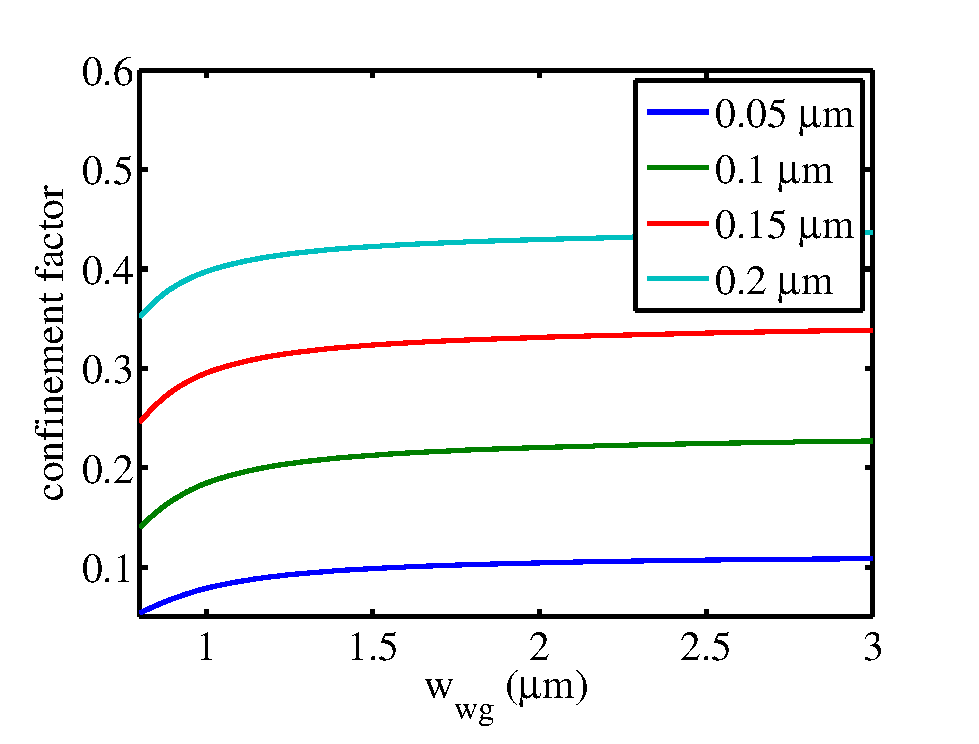
\includegraphics[width=8cm]{./Pictures/fig_ch2_ms_confinement.eps}
		\end{minipage}}
\caption{(a)-(d)分别是在不同量子阱厚度下,蘑菇型波导的$n_{neff}, n_g, loss, confinement~factor$随$w_{wg}$的关系,工作波长$\lambda_0 = ~1.55\mu m$}
\label{fig_ch2_ms_property}
\end{figure}


从图\ref{fig_ch2_ms_property}可以看到,蘑菇型等效折射率,群折射率,波导损耗,约束因子的变化趋势与矩形波导变化趋势相同。在同样的波导宽度和量子阱厚度下,蘑菇型波导的等效折射率偏大,群折射率偏小,损耗偏大,光约束能力偏小。这是由于矩形波导对光约束的更好,群折射率越大。另外蘑菇型波导相对比较宽的p-InP层,会让更多的光被上电极吸收,导致损耗偏大,光约束能力降低。

下面我们将分析蘑菇型波导的微波特性。图\ref{fig_ch2_ms_structure_mode}(c)展示了当$w_{wg} =~2 \mu m, h_{mqw} =~ 0.15 \mu m$,微波频率$f_m =40~ GHz$时的微波模场的分布,与矩形波导的微博模场分布图\ref{fig_ch2_rect_microwave_mode_equal_circuits}(a)相似,微波的大部分能量集中于MQW和SCH本征层中,部分能量集中在p-contact层。

与矩形波导分析思路相同,下面我们分析当量子阱厚度为为$0.15~ \mu m$和$0.2 ~\mu m$时蘑菇型波导的微波特性。从图\ref{fig_ch2_ms_zc}和图\ref{fig_ch2_ms_neff_ng}可以看出,当波导宽度逐渐减小或者量子阱厚度逐渐增大,蘑菇型波导的本征阻抗,微波损耗和微波等效折射率的变化趋势与矩形波导的微波特性变化趋势相同。不过,在相同波导尺寸下,这种蘑菇型波导的本征阻抗偏小,微波等效折射率偏偏大。因此,蘑菇型波导更不容易实现阻抗匹配以及微波与光波的速度匹配。
接下来,我们比较在与矩形相同波导宽度和量子阱高度下,蘑菇型波导的电光调制器带宽。当量子阱高度是$0.187~ \mu m$,波导宽度$w_{wg} = 0.8~ \mu m$工作波长为$1.55~ \mu m$时,$n_g = 3.525, loss =  2\times 10^{-3} ~dB/cm^{-1} $。此时微波的本征阻抗$Z_C$,微波损耗$loss$,微波等效折射率$n_m$随工作频率$f$的关系如图\ref{fig_ch2_ms_freq_zc}和图\ref{fig_ch2_ms_freq_neff_loss}所示。
图\ref{fig_ch2_ms_3dB}和图\ref{fig_ch2_ms_S11}分别展示了蘑菇型波导的电光响应$R_{EO}$的带宽和微波的反射系数$S_{11}$的幅值。从图\ref{fig_ch2_ms_3dB}可以看到$R_{EO}$的3~dB带宽$f_{3dB}\approx ~90 GHz$,小于矩形波导的$f_{3dB}$。并且蘑菇型波导的反射系数在25~GHz的以上时高于-25~dB,也差于矩形波导。\cite{tang2012over}。

\begin{figure}[htb]
	\small
	\subfigure[]{
		\begin{minipage}[]{0.5\textwidth}
			\centering
			\label{fig_ch2_ms_zc}
			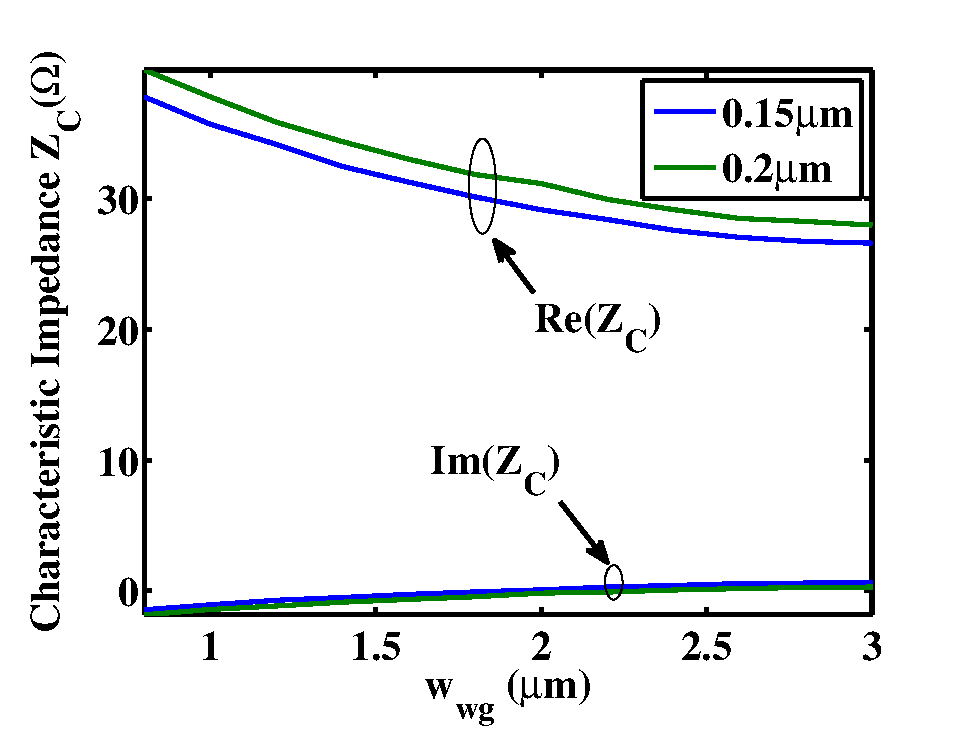
\includegraphics[width=8cm]{./Pictures/fig_ch2_ms_zc.eps}
		\end{minipage}}
		\subfigure[]{
		\begin{minipage}[]{0.5\textwidth}
			\centering
			\label{fig_ch2_ms_neff_ng} %% label for second subfigure
			\includegraphics[width=8cm]{./Pictures/fig_ch2_ms_neff_ng.eps}
		\end{minipage}}
	\subfigure[]{
		\begin{minipage}[]{0.5\textwidth}
			\centering
			\label{fig_ch2_ms_freq_zc}
			\includegraphics[width=8cm]{./Pictures/fig_ch2_ms_freq_zc.eps}
		\end{minipage}}
	\subfigure[]{
		\begin{minipage}[]{0.5\textwidth}
			\centering
			\label{fig_ch2_ms_freq_neff_loss} %% label for second subfigure
			\includegraphics[width=8cm]{./Pictures/fig_ch2_ms_freq_neff_loss.eps}
		\end{minipage}}
	\subfigure[]{
		\begin{minipage}[]{0.5\textwidth}
			\centering
			\label{fig_ch2_ms_3dB} %% label for second subfigure
			\includegraphics[width=8cm]{./Pictures/fig_ch2_ms_3dB.eps}
		\end{minipage}}
	\subfigure[]{
		\begin{minipage}[]{0.5\textwidth}
			\centering
			\label{fig_ch2_ms_S11} %% label for second subfigure
			\includegraphics[width=8cm]{./Pictures/fig_ch2_ms_S11.eps}
		\end{minipage}}
	\caption{(a), (b)分别是$f_m = 40~GHz$时,在不同量子阱厚度下,蘑菇型波导微波的本征阻抗$Z_C$,微波损耗$loss$,微波等效折射率$n_m$随$w_{wg}$的关系;(c), (d)分别是$w_{wg} = 0.8 ~\mu m, h_{mqw} = 0.187 ~\mu m$时,在不同量子阱厚度下,蘑菇型波导微波的本征阻抗$Z_C$,微波损耗$loss$,微波等效折射率$n_m$随微波频率$f$的关系;(e)蘑菇型波导调制器的电光调制器带宽$R_{EO}$;(f)蘑菇型波导调制器的微波反射系数$|S_{11}|$}
	\label{fig_ch2_ms_3dB_S11}
\end{figure}

虽然远离量子阱区域的电极尺寸的变化对光波的影响十分微弱,但是,由于微波波长尺寸大,电极尺寸的变化对微波的特性影响十分明显。在此,我们分析地电极和源电极的尺寸变化对波导微波性能的影响。通过表\ref{rect_metal_influence}的分析,我们可以通过微调电极的尺寸,在不影响光波损耗的前提下,调节电极尺寸改善波导的微波特性。	
{
	\begin{table}[htb]
		\zihao{5}
		\caption{矩形或者蘑菇型波导结构,当源电极的厚度,高度,地电极的厚度和两者之间的距离变大时,微波的本征阻抗,损耗和等效折射率的变化}
		\label{rect_metal_influence}
		\centering
		\begin{tabular}[t]{lllll}
			\hline
			参数类型 &源电极的厚度 & 源电极的宽度 & 地电极的厚度& 地电极之间的距离 \\
			\hline
			本征阻抗 &   减小 & 减小 & 减小 &增大\\
			损耗  &   减小 & 减小 & 增大 &增大\\
			等效折射率 &  减小 & 减小 & 减小 &增大\\
			\hline
		\end{tabular}
	\end{table}
}

			
\section{本章小结}
在本章中,我们详细介绍了设计硅基混合集成III-V波导的两个方面。第一方米我们首先详细介绍III-V外延片量子阱结构的吸收谱计算的四个步骤。然后对于设计量子阱,这种多参数优化问题,我们首次引入了利用退火算法设计、优化量子阱结构的思路。通过合理设计退火算法中参数的取值范围,以及退火算法的权值函数,我们可以快速设计出偏振不敏感的电吸收光调制器的量子阱结构。最后,我们总结了III-V外延片的总体设计。第二方面是混合集成III-V波导尺寸尺寸的设计,我们分析了两种类型的波导,矩形波导和蘑菇型波导分析了波导宽度和多量子阱高度对波导光学和微波特性的影响,并且分析了相同尺寸下,两种结构的电光调制带宽。我们发现在相同尺寸下矩形波导可以实现阻抗匹配,而蘑菇型波导本征阻抗偏小,这导致了矩形波导可以实现$f_{3dB} = 100~GHz$的调制带宽。

\chapter{硅波导和混合集成III-V波导的模式耦合}
\section{背景介绍}
硅基混合集成III-V平台光器件的一个共性问题就是混合集成III-V波导和硅波导模式的耦合。硅波导和硅基混合集成III-V波导的模式如图\ref{fig_ch3_si_hybrid_mode}所示,在能量分布和等效折射率上都有很大的差别。目前,采用的方案是利用锥形(taper)结构。在硅波导的锥形结构上,宽度逐渐减小,而对应的III-V波导上宽度则逐渐增大,从而使硅波导上的光缓慢耦合到III-V波导中。图\ref{fig_ch3_background_str}(a, b)展示了目前采用的用于硅波导和混合集成III-V波导的多层或者多段锥形耦合结构\cite{kurczveil2013characterization, keyvaninia2009engineering}。这些耦合结构的尺寸都在40 ~$\mu m$以上,被广泛用于混合集成的激光器,探测器和调制器。由于光器件的小型化,能增加光器件的集成度,降低单个光器件的成本,所以目前硅基光子器件的一个趋势是将原先的器件的尺寸缩小。为此,文献[\citenum{wang2012heterogeneous}]将线性锥形结构变为曲形锥形结构,如图\ref{fig_ch3_background_str}(c)所示,将耦合结构尺寸缩小到了$25~\mu m$。不过,并没说明耦合结构是否还可以进一步减小。
\begin{figure}[htb]
	\small
	\subfigure[]{
		\begin{minipage}[]{0.5\textwidth}
			\centering
			\label{fig_ch3_si_mode}
			\includegraphics[width=6cm]{./Pictures/fig_ch3_si_mode.eps}
		\end{minipage}}
	\subfigure[]{
		\begin{minipage}[]{0.5\textwidth}
			\centering
			\label{fig_ch3_hybrid_mode} %% label for second subfigure
			\includegraphics[width=6cm]{./Pictures/fig_ch3_hybrid_mode.eps}
		\end{minipage}}
	\caption{(a) $600~nm$宽硅波导的模式,其等效折射率$n_{eff}=2.58$;(b) $1~\mu m$宽硅基混合集成III-V波导的模式,其等效折射率$n_{eff}=3.19$}
	\label{fig_ch3_si_hybrid_mode}	
\end{figure}
		
\begin{figure}[htb]
	\centering
	\includegraphics[width=12cm]{./Pictures/fig_ch3_background_str.jpg}
	\caption{ 目前硅波导和混合集成III-V波导的模式耦合结构(a) 多层锥形耦合结构\cite{kurczveil2013characterization};(b)多段锥形耦合结构\cite{keyvaninia2009engineering};(c)曲形锥形结构\cite{wang2012heterogeneous}}
	\label{fig_ch3_background_str}
\end{figure}

我们在尝试减小耦合尺寸时,首次发现限制耦合长度的重要因素是来自于III-V波导的高阶模式,我们通过设计三段式耦合结构,充分利用III-V材料选择性刻蚀的特点,形成近似三维锥形结构,将光缓慢地从硅波导耦合到III-V波导中。通过这种方法我们设计了长度只有8~$\mu m$的导耦合结构。这个结构能实现了95\%以上的能量耦合,并且相应带宽也能达到100 nm。随后我们探索了用电子书光刻(Electron Beam Lithography, E-Beam)制作这种紧凑耦合结构的工艺流程。
\section{紧凑型三段式耦合结构的设计}
为了验证这种紧凑型三段式耦合结构的设计方法,我们采用的III-V材料厚度和折射率如表\ref{IIIV_qian_str}与文献[\citenum{wang2012heterogeneous}]相同。这样也便于比较我们的设计思路。硅基混合集成III-V波导的截面示意图如图\ref{fig_ch3_3d_taper}(a)所示。硅波导的上表面和III-V的下表面我们定义为键合层的厚度为$h_{BCB}$。
{
	\begin{table}[htb]
		\zihao{5}
		\caption{III-V材料各层的厚度和折射率\cite{wang2012heterogeneous}}
		\label{IIIV_qian_str}
		\centering
		\begin{tabular}[t]{lll}
			\hline
			名称  & 厚度~$(\mu m)$  & 折射率 \\
			\hline
			DVS-BCB & - & 1.543\\
			p-cladding & 1.5 &3.17 \\
			SCH & 0.08 & 3.46 \\
			MQW & 0.1 & 3.52 \\
			SCH & 0.12 & 3.46 \\
			n-contact & 0.14 & 3.17 \\
			Si & 0.22 & 3.477 \\
			SiO2 & 1 & 1.45 \\
			\hline
		\end{tabular}
	\end{table}
}

\begin{figure}[htb]
	\centering
	\includegraphics[width=12cm]{./Pictures/fig_ch3_3d_taper.jpg}
	\caption{紧凑型三段锥形耦合器的结构图:(a) 波导剖面图;(b)俯视图;(c)三维立体视图}
	\label{fig_ch3_3d_taper}
\end{figure}


图\ref{fig_ch3_3d_taper}(b)和\ref{fig_ch3_3d_taper}(c)展示了所提出的锥形耦合结构的示意图。从图中可以看出了,锥形耦合结构分成了三段结构。在第一段结构中,光从硅波导首先耦合到0.44~$\mu m$厚的由两个SCH层,MQW层和n-contact层构成的III-V波导中。在第二段结构中,0.44~$\mu m$厚的III-V波导的宽度逐渐增加,提高光在MQW层的限制能力。在第二段结构的末尾光的模场已经和最终所需的模式几乎相匹配。因此在第三段结构,我们可以将最厚的p-cladding层通过一个很短的锥形结构引入。通过三段式的锥形耦合结构,可以将整个模式耦合的长度大大缩短。

两根垂直分离的波导中两个模式相互耦合的问题已经在文献[\citenum{sun2009adiabaticity}]中进行详细的理论分析,并且给出了最短耦合长度的解析解。当两根分立波导的模式所对应的等效折射率随波导的长度有相交,并且两个光场模式的对称性相同时,那么两个波导靠近,就会有光模式的相互耦合。然而,文献[\citenum{sun2009adiabaticity}]的理论中,仅考虑了每根波导只有基模的情况。然而,实际中III-V波导,却拥有很多高阶模式。如果在耦合结构中,这些高阶模式的等效折射率变化也和硅波导的等效折射率变化有所相交,那么硅波导的部分光能量就会耦合到III-V波导的高阶模式中去。

图\ref{fig_ch3_multimode}(a)展示了,当p-cladding存在时的传统III-V波导模式的等效折射率$(n_{eff})$随波导宽度变化的关系。我们可以看到此时III-V支持很多高阶模式,并且高阶模式和基模之间的等效折射率差很小。另外一方面,从图\ref{fig_ch3_multimode}(b),我们可以看到当III-V波导没有很厚的p-cladding时,III-V波导只支持相对较少的模式。此时高阶模式和基模等效折射率的差距,见图\ref{fig_ch3_multimode}(b),也比之前有所提高。这意味着,在硅波导的基模转化成III-V波导的基模时,III-V波导高阶模式的影响就明显减弱。因此,利用没有p-cladding层的III-V波导,可以实现硅和III-V之间紧凑的耦合结构。这种三段式锥形结构不仅拥有多层锥形耦合结构少反射率的特点\cite{kurczveil2013characterization},也利用第一段的没有p-cladding III-V锥形波导阻止了高阶模式的产生。通过将整个锥形耦合结构分成独立的三段,我们可以对每段锥形耦合结构单独的优化。接下来,我们就讨论每段taper的优化过程。

\begin{figure}[htb]
	\centering
	\includegraphics[width=12cm]{./Pictures/fig_ch3_multimode.jpg}
	\caption{模式等效折射率$n_{eff}$随着III-V波导宽度的变化:(a) III-V波导包含p-cladding层;(b)III-V波导没有p-cladding层}
	\label{fig_ch3_multimode}
\end{figure}

三段式的锥形耦合结构可以通过选择性湿法腐蚀的工艺制作,这个方法也被用于制作多层锥形结构\cite{kurczveil2013characterization}。图\ref{fig_ch3_detail_structure}展示了详细的设计结构参数。所有锥形结构的尖端宽度$(W_{tip})$受到工艺的限制。更细小的尖端意味着更小的反射。在此,我们同文献[\citenum{wang2012heterogeneous}]相同,$W_{tip} = 0.15~\mu m$。输入硅波导的宽度是$0.6~\mu m$。在第三段锥形结构中,最后的硅基混合集成III-V波导的MQW层的宽度$W_{mqw2}$与p-cladding的宽度$W_{pInP}$相同,我们在此选取$W_{mqw2}$为最后波导的宽度。$W_{mqw2}$是通过优化光的约束因子来确定。图\ref{fig_ch3_confinement}展示了在$W_{mqw2}$变化时,100 nm厚的MQW层对光的约束因子。我们可以看到当$W_{mqw2} > 0.5~\mu m$时,光的限制因子已经趋于稳定。在此,我们选取$W_{mqw2} = 1 ~\mu m$,此时,光限制因子已经达到25\%的稳定值。

\begin{figure}[htb]
	\centering
	\includegraphics[width=12cm]{./Pictures/fig_ch3_detail_structure.jpg}
	\caption{三段式波导详细的结构参数:(a) 第一段垂直耦合结构;(b)第二段结构;(c)第三段结构}
	\label{fig_ch3_detail_structure}
\end{figure}

\begin{figure}[htb]
	\centering
	\includegraphics[width=12cm]{./Pictures/fig_ch3_confinement.jpg}
	\caption{光在100 nm厚量子阱区域的限制因子}
	\label{fig_ch3_confinement}
\end{figure}

在每段锥形结构的轮廓我们采用文献[\citenum{sun2009adiabaticity}]中的多项式进行描述\ref{Equ:exponential}:
\begin{equation}
\label{Equ:exponential}
W(x) = w_0+(w_1+w_0)\left(x/L_t\right)^\alpha
\end{equation}
其中,$W(x)$是$x$处的宽度,$w_0$是初始宽度,$w_1$是末尾宽度,$L_t$是锥形结构的长度,$\alpha$是指数项用于定义锥形结构的外形。由于实际工艺中,SCH层和MQW层的材料不能选择性腐蚀,因此他们的形状在此设计中是相同的。为了简化设计,MQW层和n-contact层的指数项$\alpha$保持相同。

在第一段锥形结构中,我们首先选择MQW层锥形结构末端的宽度。从图\ref{fig_ch3_multimode}(b),我们可以看到,当MQW的宽度为$0.5 ~ \mu m$时,基模的等效折射率和高阶模式的等效折射率差别最大,因此我们将其设置为$0.5 ~ \mu m$。由于很薄的n-contact层对模式的影响很小。在这个例子中,我们将n-contact锥形结构末端的宽度设置为$1.5 \mu m$。除此,在第一段锥形结构中,还有3个参数需要设计优化,即锥形结构的长度$L_1$,定义硅锥形结构外形的指数项$\alpha_{si}$和定义III-V锥形结构外形的指数项$\alpha_1$。

在第二段锥形结构中,MQW层末端的宽度与最后硅基混合集成III-V波导的宽度相同,即$W_{mqw2} = 1~\mu m$。我们将n-contact锥形结构的末端设置为$3~\mu m$。除此之外,还有两个参数需要优化,即锥形结构的长度$L_2$以及III-V锥形结构外形的指数项$\alpha_2$。

在第三段锥形结构中,MQW层波导的宽度不变为$1~\mu m$,而p-cladding锥形结构末尾宽度也为$1~\mu m$。而锥形结构的长度$L_3$和p-cladding锥形外形的指数项$\alpha_3$,这两个参数需要进一步优化。

我们采用三维的时域有限差分方法(3D Finite-Difference Time domain method, 3D-FDTD)软件去仿真各段锥形结构的耦合效率\cite{fdtdsolution}。通过分别优化每段的结构参数,实现最高的基模耦合效率。然后,将优化的每段结构在组合成整体结构。一般采用DVS-BCB键合的厚度$h_{BCB}$可以达到30 nm至100 nm。在此,我们选择$h_{BCB} = 50~nm$。之前各段锥形结构中待优化的参数,我们通过扫描,仿真结果见图\ref{fig_ch3_sweep_structure}。我们可以看到硅锥形结构的指数项$\alpha_{si}$对耦合效果没有明显影响。然而,其他的指数项$\alpha_1$,$\alpha_2$,$\alpha_3$对耦合效率有明显的影响。根据图\ref{fig_ch3_sweep_structure}(a)-\ref{fig_ch3_sweep_structure}(c),我们选取$\alpha_{si} = 2.2$,$\alpha_1 = 0.6$,$\alpha_2 = 0.6$,$ \alpha_3 = 0.9$。在扫描指数项时,锥形结构必须有足够的长度。接下来,在确定最佳锥形结构外形时,我们扫描锥形结构的长度。从图\ref{fig_ch3_sweep_structure}(d)到图\ref{fig_ch3_sweep_structure}(f),我们可以看到,当$L_1 = 4~ \mu m$, $L_2 = 1~\mu m$,$ L_3 =  3~\mu m $时,耦合效率已经达到96\%以上,继续增加长度,耦合效率只有3\%的波动。这保证了每段锥形结构都是绝热的。因此,整体锥形结构的长度只$有8 \mu m$。

\begin{figure}[htb]
	\centering
	\includegraphics[width=14cm]{./Pictures/fig_ch3_sweep_structure.jpg}
	\caption{各段锥形耦合结构在不同结构参数下的耦合效率:(a)当第一段的锥形结构的长度$L_1 = 4~\mu m$;(b)当第二段的锥形结构的长度$L_2 = 4~\mu m$;(c)当第三段的锥形结构的长度$L_1 = 3~\mu m$;(d)当第一段的锥形结构中$\alpha_{si}= 2.2$,$\alpha_1 = 0.6$;(e)当第一段的锥形结构中$\alpha_2 = 0.6$;(f)当第三段的锥形结构中$\alpha_1 = 0.9$}
	\label{fig_ch3_sweep_structure}
\end{figure}

图\ref{fig_ch3_8um_taper}展示了三段式锥形结构的仿真结果。从图\ref{fig_ch3_8um_taper}(a)可以看到,当基模的耦合效率达到95\%上时,对应的波长带宽达到了100 nm。 当基模的耦合效率达到90\%上时,对应的波长带宽达到了300 nm。从图\ref{fig_ch3_8um_taper}(a)也可以看出,在短波长,第一段锥形结的损耗构限制了耦合效率。在长波长,却是第三段锥形结构的损耗限制了耦合效率。在图\ref{fig_ch3_8um_taper}(b),我们分析了不同$h_{BCB}$下,耦合效率的变化。可以看到$8 ~\mu m$长的锥形结构在$h_{BCB}$从20 nm变化到80 nm时,耦合效率依旧保持在90\%以上。图\ref{fig_ch3_8um_taper}(c)展示了在工作波长$1.55~\mu m$,$h_{BCB} =  50 ~nm$时,光场从硅波导耦合到硅基混合集成III-V波导的模式耦合图。可以看到,光在两个波导之间的相互耦合主要发生在第一段锥形结构。因此,第一段锥形结构对$h_{BCB}$的变化十分敏感。当光耦合到III-V后,$h_{BCB}$的变化就几乎不会影响光场的变化,因此第二段和第三段锥形结构几乎不影响锥形结构的耦合效率。而在图\ref{fig_ch3_8um_taper}(b)中,也展示了$h_{BCB}$的变化对第一段锥形结构的耦合效率影响最大。

\begin{figure}[htb]
	\centering
	\includegraphics[width=14cm]{./Pictures/fig_ch3_8um_taper.jpg}
	\caption{$8~\mu m$耦合结构的性能:(a)当$h_{BCB}=50~nm$时,波长变化对耦合效率的影响;(b)当工作波长为$1550~nm$时,$h_{BCB}$变化的影响;(c)当工作波长为$1550~nm$,$h_{BCB}=50~nm$时,模场在耦合结构中的传播图;(d)当p-cladding层出现套刻误差的影响;(e)当MQW层和SCH层出现套刻误差的影响;(f)当n-contact层出现套刻误差的影响}
	\label{fig_ch3_8um_taper}
\end{figure}

加工这三段式的耦合结构需要三次掩膜版的套刻工艺。它们分别用于定义p-cladding层,MQW层和SCH层,以及n-contact层。因此,我们进一步分析了掩膜版套刻偏离对耦合效率的影响。从图\ref{fig_ch3_8um_taper}(d)可以看到,p-cladding层的套刻偏离只会影响第三段锥形结构的耦合效率。这是由于p-cladding只存在于第三段锥形耦合结构中。从图\ref{fig_ch3_8um_taper}(e)可以看出,MQW层和SCH层的套刻偏离对第一段和最后一段耦合结构的耦合效率有明显的影响,并且MQW层和SCH层的套刻偏差是对整体耦合结构效率的影响最大的。从图\ref{fig_ch3_8um_taper}(f)可以看出,n-contact层的套刻偏差对整体耦合效率只有微弱的影响。基于以上的分析,为了使$8 \mu m$长的耦合结构保持90\%以上的耦合效率,MQW层和SCH层的套刻精度需要保持在100~nm的范围内。

为了增加耦合结构的光学带宽,对$h_{BCB}$变化的容忍度和对掩膜套刻精度的容忍度,第一段和最后一段耦合结构的耦合效率需要提高。其中一个简单的方式是通过增加耦合结构的长度。我们将$L_1$增加到了$8~\mu m$,并且将$L_3$增加到了$5~\mu m$,并且保持其他的参数不变。整个耦合结构的长度增加到了$14~\mu m$。这个增长的锥形耦合结构的仿真结果如图\ref{fig_ch3_14um_taper}所示。

从图\ref{fig_ch3_14um_taper}(a)可以看出,这个增长耦合结构的模式耦合效率在95\%以上,对应的波长范围达到了200 nm。在90\%以上耦合效率的波长范围达到了500 nm。从图\ref{fig_ch3_14um_taper}(b)可以看到,当$h_{BCB}$从0 nm变化到100 nm时,整个耦合结构的耦合效率依旧能保持在95\%以上。图\ref{fig_ch3_14um_taper}(c)展示了当工作波长为$1.55 ~\mu m, h_{BCB} = 50~nm$时,在这$14~\mu m$长耦合结构的模场传播图。

从图\ref{fig_ch3_14um_taper}(d)到图\ref{fig_ch3_14um_taper}(f)展示了每层掩膜版套刻误差对这个$14~\mu m$长锥形结构的耦合效率的影响。通过与之前图\ref{fig_ch3_8um_taper}(d)至图\ref{fig_ch3_8um_taper}(f)的比较,我们可以看到长度增加的锥形结构对工艺中套刻误差的容忍度更高。当p-cladding层的套刻误差在$\pm 200~nm$的范围内,当MQW层和SCH层的套刻误差在$\pm 100~nm$的范围内,当n-contact层的套刻误差在$\pm 150~nm$的范围内时,整个锥形结构的耦合效率依旧能保持在95\%以上。通过之前的讨论分析,我们可以发现第二段锥形结构中MQW层和SCH层掩膜的套刻精度对整个锥形结构的偶耦合效率影响最大。

\begin{figure}[htb]
	\centering
	\includegraphics[width=14cm]{./Pictures/fig_ch3_14um_taper.jpg}
	\caption{$14~\mu m$长耦合结构的性能:(a)当$h_{BCB}=50~nm$时,波长变化对耦合效率的影响;(b)当工作波长为$1550~nm$时,$h_{BCB}$变化的影响;(c)当工作波长为$1550~nm$,$h_{BCB}=50~nm$时,模场在耦合结构中的传播图;(d)当p-cladding层出现套刻误差的影响;(e)当MQW层和SCH层出现套刻误差的影响;(f)当n-contact层出现套刻误差的影响}
	\label{fig_ch3_14um_taper}
\end{figure}

通常而言,硅基混合III-V平台中的调制器相比激光器和放大器,不需要高的耦合效率。因此,$8~\mu m$长的耦合结构非常适合硅基光调制器。而对于激光器和光放大器,由于三段式后结构的第一段没有p-cladding层,所以无法进行有效的电泵浦。又因为激光器和光放大器的MQW的吸收峰就落在其激光出射的波段,因此第一段耦合结构可能带来比较大的损耗。而对于电吸收光调制器,在没有电压下的MQW的吸收峰是小于工作波长的,因此就没有这个问题。文献[\citenum{tang201150,tang2012energy,tang2012over}]中特意用离子注入对锥形耦合结构进行电学隔离,而在我们所提出的三段式耦合结构中,我们通过在一段锥形结构中去除了p-cladding层,自然而然地进行了电学的隔离。

\section{紧凑三段式耦合结构的工艺探索}
紧凑型三段式耦合结构可以用于硅基混合集成III-V平台下使用矩形波导结构的电吸收光调制器。根据上章分析,这种调制器具有调制带宽大的特点。而目前硅基混合集成III-V的电吸收光调制器都是蘑菇型波导,由于其波导宽度大于$1~\mu m$,定义波导图形是采用接触式光刻。而在矩形波导的光调制器以及三段式耦合结构中,波导宽度都需要小于$1~\mu m$。因此,这种结构无法用现有的接触式光刻制作。

在此我们首次尝试用电子束光刻制作三段式耦合结构。虽然电子束光刻已经在实验室中被广泛用于制作纯硅光器件,但是没有被用于制作硅基混合集成III-V波导。其中两个主要原因是,电子束的光刻胶的厚度比较薄,和电子束容易被散射的问题。如图\ref{fig_ch3_ele_sca}(a),如果片子表面的局部高度起伏大于光刻胶的厚度,那么将会严重影响光刻胶的表面的平整度,从而影响定义图形的精确尺寸。图\ref{fig_ch3_ele_sca}(b)展示了在一个陡直的侧壁附近套刻图形,那么电子束就会被侧壁散射,从而使图形展宽。
\begin{figure}[htb]
	\centering
	\includegraphics[width=12cm]{./Pictures/fig_ch3_ele_sca.jpg}
	\caption{(a)片子局部表面起伏太大,导致光刻胶匀完后表面不平整;(b)陡直侧壁处套刻图形,导致电子被散射,使曝光图形展宽}
	\label{fig_ch3_ele_sca}
\end{figure}

电子束胶的厚度普遍小于1~$\mu m$,适合用于套刻和定义波导高度差普遍小于500~nm的纯硅光器件图形。然而在硅基混合集成III-V平台上,波导的高度差会达到2~$\mu m$。尤其在制作三段式耦合结构中,套刻第二层锥形结构时,需要在高度1.5~$\mu m$的p-cladding上再精确地套刻MQW层和SCH层的图形。这将会遇到定义图形展宽,变形的问题。下面将详细介绍工艺步骤解决这两个问题。

第一步定义p-cladding层图形,如图\ref{fig_ch3_step1_2}(a)所示。我们首先在混合集成的III-V外延片上用等离子体增强化学气相沉积(Plasma Induced Chemical Vapor Deposition,PECVD)生长一层300~nm-400~nm厚的二氧化硅(SiO\SB{2})。在生长之前,需要将片子在温度100摄氏度以上的热盘上,放置3min,使表面和背面的水汽蒸发,以防片子放入PECVD,片子滑动。在匀电子束胶之前,SiO\SB{2}表面需要用增粘剂处理,使其与ma-N 2403的粘附性增强。我们是将长完二氧化硅的片子,用甲烷轰击,以提高其和ma-N 2403的粘附性。然后,再匀电子光刻胶ma-N 2403\cite{man2403}。这是一种负胶,厚度大概300 nm左右。紧接着,我们将其放到90摄氏度的热盘上90 s。做完这步,就意味着我们的片子已经准备好放入电子束光刻机中曝光了。根据图形的最小尺寸和胶的特性,选用相应的电场强度和孔径的电子枪,从而使图形写的时间短并且精度满足要求。我们使用电场强度为30~KV,孔径为20~$\mu m$的电子枪。除此之外,不同图形的面积,形状,需要不同的曝光计量,和电子束移动的方式。这个需要根据不同材料,不同光刻胶,调整。我们写完图形后,用显影液ma-D525显影2分30秒。最后为了使光刻胶侧壁光滑些,我们将其放入110摄氏度的烘箱中,将光刻胶进行回流,从而减小光刻胶侧壁的粗糙度。

第二步将光刻胶的图形转移到p-cladding层,如图\ref{fig_ch3_step1_2}(b)所示。定义好光刻图形后,我们将片子背面涂上导热胶,放到感应耦合等离子体刻蚀机(Inductively Coupled Plasma, ICP)中,利用CH\SB{3} : CF\SB{4} = 50 : 6的混合气体,在3~mT的压强,在适当的射频功率下,进行刻蚀。刻蚀结束后,由于光刻胶已经被碳化,无法用丙酮去除干净。在此,我们用强力去胶剂(N-甲基吡咯烷酮)将残留的光刻胶去除干净,再把片子放入利用氧等离子体的去胶机中,将残留的光刻胶彻底取出干净。此时,图形已经转移到二氧化硅上。接下来,我们ICP刻蚀p-contact(材料为InGaAs) 层和p-cladding(材料为InP)层。此时ICP的中的混合气体是H\SB{2}:Cl\SB{2}:CH\SB{4}:Ar = 5:7:10:5,腔内温度为60摄氏度,压强为4~mT。由于ICP不是选择性刻蚀,会同时刻蚀SCH和p-cladding层。为此,我们根据刻蚀速率,当InP还剩下100-300 nm时,换成湿法腐蚀。我们采用HCl:H\SB{2}O = 1:1的溶液在20摄氏度下腐蚀InP。此时的腐蚀速率大概100~nm/min。腐蚀后,在显微镜下观察片子表面颜色是否均匀,表面是否光滑。此时在波导外,片子的上表面是SCH层。最后,我们将片子放入BOE (Buffered Oxide Etch,HF:NH\SB{4}F=1:6)的溶液中,去除二氧化硅掩膜。实际片子的腐蚀电镜图见图\ref{fig_ch3_step1_2}(c)。

\begin{figure}[htb]
	\centering
	\includegraphics[width=14cm]{./Pictures/fig_ch3_step1_2.jpg}
	\caption{(a)第一步结束后的波导截面示意图;(b)第二步结束后的波导截面示意图;(c)第二步结束后器件的电镜俯视图}
	\label{fig_ch3_step1_2}
\end{figure}

第三步套刻MQW层和SCH层的图形,如图\ref{fig_ch3_step3_4}(a)所示。接下来,我们需要再利用PECVD沉积一层300nm左右的二氧化硅。从图\ref{fig_ch3_step3_4}(b)可以看到沉积的二氧化硅也会把波导的侧壁包裹住。接下来,与步骤一的匀胶过程一样,对SiO\SB{2}进行表面处理提高其对光刻胶的粘附性。在此我们使用正胶ZEP~520套刻图形\cite{ZEP520},而不是负胶。如果使用负胶的话,定义图形时,就会出现之前所述的电子被波导的侧壁散射的问题,如图\ref{fig_ch3_ele_sca}(b)所示。实际中被电子散射展宽的波导如图\ref{fig_ch3_step3_4}(c)所示。而采用正胶时,电子束写图形外侧的光刻胶,避免了与波导侧壁的接触,从而可以在波导附近套刻出精准的图形。我们将图形定义的宽度稍微比实际的宽度偏大500~nm左右,通过下一步的湿法腐蚀,将这个宽度余量弥补回来。旋涂完ZEP胶,我们将其放在180摄氏度的热板上10分钟。至此片子可以放入电子束光刻机中写图形了。我们使用电场强度为30~KV,孔径为20~$\mu m$的电子枪套刻图形。套刻完图形后,我们将其放到显影液中显影,然后进行定影。最后,提高光刻胶与二氧化硅的刻蚀比,我们其放到60到120摄氏度的缓慢升温的热盘上10分钟,对光刻胶硬化。

第四步将光刻胶的图形转移到MQW层和SCH层,如图\ref{fig_ch3_step3_4}(d)所示。首先与第二步相同,ICP刻蚀SiO\SB{2}。然后,然后利用强力去胶剂和氧等离子体的去胶机,将残留的光刻胶彻底去除干净。接下来,就是将图形从SiO\SB{2}上转移到MQW层和SCH层。由于MQW和SCH的成分是InAlGaAs,因此我们使用柠檬酸(citric) : H\SB{2}O\SB{2} = 20 : 1的溶液,在室温下进行腐蚀。每隔5分钟测量腐蚀深度,确定腐蚀速率。我们适当过腐蚀,进行内刻蚀(undercut)将波导宽度缩小到设计值。最后,我们将片子放入BOE溶液中,去除二氧化硅掩膜。此时的波导如图,如图\ref{fig_ch3_step3_4}(e)所示。

\begin{figure}[htb]
	\centering
	\includegraphics[width=14cm]{./Pictures/fig_ch3_step3_4.jpg}
	\caption{(a)第三步结束后的波导截面示意图;(b)二氧化硅包裹着的波导截面电镜图;(c)用负胶套刻,导致图形展宽的电镜图;(d)第四步结束后的波导截面示意图;(e)第四步结束后的器件电镜俯视图}
	\label{fig_ch3_step3_4}
\end{figure}


第五步套刻n-contact层的图形,如图\ref{fig_ch3_step5_6}(a)所示。与第三步相同,首先利用PECVD沉积一层300 nm左右的二氧化硅膜。再对SiO\SB{2}表面处理提高其对光刻胶的粘附性。我们在此也使用正胶ZEP 520套刻图形。旋涂完ZEP胶,前烘180摄氏度的热板上10分钟。接下来电子束光刻机配置电场强度为30~KV,孔径为20~$\mu m$的电子枪,套刻图形。结束后放到显影液中显影,然后进行定影。最后,后烘片子,将其放置在60到120摄氏度缓慢升温的热盘上10分钟,提高光刻胶与二氧化硅的刻蚀比。

第六步将光刻胶的图形转移到n-contact层,如图\ref{fig_ch3_step5_6}(b)所示。与第二步相同,ICP刻蚀SiO\SB{2}。然后利用强力去胶剂和氧等离子体的去胶机,将残留的光刻胶彻底去除干净。接下来,将片子放入ICP进行刻蚀。n-contact层也是InP,因此配方与第二步中描述的一样。刻蚀完InP后,,我们将片子放入BOE溶液中,去除二氧化硅掩膜。至此,使用电子束光刻制作三段式耦合结构已经完成,如图\ref{fig_ch3_step5_6}(c)所示。由于ICP可是InP的洁净度要求很高,最好单个ICP刻蚀两三种材料相似的材料,否则会把ICP墙体弄脏。如果腔体肮脏的话,可能会很难清洗,就会使刻蚀完的结构产生如图\ref{fig_ch3_step5_6}(c)所示的小的脏颗粒。
\begin{figure}[htb]
	\centering
	\includegraphics[width=14cm]{./Pictures/fig_ch3_step5_6.jpg}
	\caption{(a)第五步结束后的波导截面示意图;(b)第六步结束后的波导截面示意图;(c)第六步结束后的器件电镜俯视图}
	\label{fig_ch3_step5_6}
\end{figure}

由于我们实验室中只有一台刻蚀III-V材料的ICP,由于ICP腔体受到污染,导致干法刻出的三段式耦合结构周围附着无法清除的脏颗粒。另外我们考虑到电子束光刻机和干法刻蚀仪器不仅设备昂贵,而且制作成本也高,所以,接下来我们采用加工成本低廉的接触式光刻和纯湿法工艺,制作改进型的混合集成III-V波导和硅波导的耦合结构。在下一章,我们将详细介绍其结构和工艺流程。
\section{本章小结}
在本章中,我们解决硅基混合平台中硅波导和混合集成III-V波导的耦合问题。并且我们分析了限制硅波导和混合集成III-V波导耦合器件长度的原因,是来自于III-V波导的高阶模式容易在光耦合的过程中被激发出来。为此,我们设计了三段式锥形耦合结构,实现了长度只有$8 ~\mu m$的耦合结构。这是目前最小的耦合结构,基模的耦合效率能达到95\%,对应的工作波长带宽具有100~nm。这种结构能增加硅基混合集成III-V器件的集成度。除此之外,考虑到实际工艺问题,我们进一步分析了制作过程中,套刻精度和硅与III-V键合层厚度的对耦合效率的影响。我们发现MQW层和SCH层的套刻精度对波导的耦合效率影响最为明显。最后,我们首次探索利用电子束光刻定义和套刻这种三段式锥形结构的工艺流程。通过巧妙地利用正胶,曝光的胶保留下来的性质,解决了由于电子束在高度落差大的波导附近套刻,出现由电子被波导侧壁反射而导致的线形展宽的问题。最后,我们初步实现了利用电子束光刻机在硅基混合集成III-V平台上制作了三段式锥形耦合的结构。不过,由于我们实验设备的缺陷,无法制作出洁净的三段式耦合结构,在下一章,我们将采用新的工艺,通过接触式光刻和湿法腐蚀方式制作混合集成III-V波导和硅波导的耦合结构。

\chapter{低驱动电压硅基混合集成电吸收光调制器}
基于QCSE效应的电吸收光调制器具有高速,低能耗,高消光比和小尺寸的特别点\cite{tang2012energy, fukano2006very}。因此电吸收光调制器被广泛应用于光通信领域。另外,电吸收光调制器具有双工作模,还可以被用于高速的光探测器\cite{welstand1996dual}。基于这个特性,研究人员实现了光电振荡器(Optoelectronic Oscillators, OEO)\cite{zhou2014compact}。我们最近也实现了单片集成的光收发器\cite{chen2016wavelength}。最近,由于硅光子和晶体管可以在统一的半导体工艺线上制作。这给复杂的光电集成系统,比如集成光子微波系统\cite{Marpaung2013integrated}和芯片间的光互联系统\cite{sun2015single},带来了希望。基于硅和III-V的键合技术,已经实现硅基混合集成III-V光调制器\cite{kuo2008high,tang201150,tang2012over,tang2012energy,chen2011forty,Srinivasan2012micro,fu20155}。不过,硅基光芯片中,低能耗是十分重要的指标。又因为电吸收光调制器的驱动电压与能耗成平方关系,见公式\ref{Equ:EC}。因此,硅基光芯片中低驱动电压的光调制器十分重要。另外,如果电吸收光调制器能够直接被来自逻辑电路的低电压信号驱动,那么消耗于电的放大器的能量也会被节省下来。最近,研究人员们在纯硅上展示了100~mV以下的硅基光调制器,见表格\ref{sil_mod}。然而,这些硅的调制器都是基于光的谐振腔结构,见图\ref{fig_mod_opt_type}(a)所示,它们对工艺的要求十分苛刻,并且还不能用于光探测器。对于传统的基于QCSE的电吸收光调制器,降低驱动电压的同时保持同样的尺寸和插入损耗十分困难。尽管研究人员利用复杂的基于慢光效应的布拉格波导\cite{gulow-voltage2013},降低了电吸收光调制器的驱动电压,但是这种结构的光调制器不仅无法和硅光子器件集成也无法将驱动电压降低到硅调制器的层次。因此,我们需要寻找一种新的思路实现低驱动电压的光调制器。

本章概述了基于能带填充效应的新型低驱动电吸收光调制器,首先介绍了低驱动电压电吸收光调制器的原理。接着阐述了设计和和仿真结果。然后,详细介绍了制作调制器的步骤。最后,在搭建的高速光调制器测试平台上,对低驱动电压光调制器的性能进行了测试。
\section{低驱动电压光调制器的原理}
\begin{figure}[htb]
	\centering
	\includegraphics[width=14cm]{./Pictures/fig_ch4_bandfilling_diag.jpg}
	\caption{ 量子阱的能带和波函数的示意图(a)有外界反向电场下;(b)在外界无电场的时候;(c)在外界正向电子子注入的时候}
	\label{fig_ch4_band_lineup}
\end{figure}
调制掺杂中的多量子阱 (Modulation-doped Multiple Quantum-wells) 中的能带填充效应在80年代已经被深入研究\cite{livescu1988free}。能带填充效应与QCSE效应的原理示意图见图\ref{fig_ch4_band_lineup}。当正向电子注入多量子阱中势阱的导带时,相应的电子准费米能级就被提高。当电子的准费米能级高过导带中最低的能级时,即最低的能级被二维电子气体填充慢时,导致了原本激子吸收峰对应的光子无法被吸收,因此其产生的电子无法跃迁到最低的能级处。这意味着只有更高能量的光子才会被吸收,使产生电子跃迁到准费米能级处。可以预测随着注入电子浓度的增加,使电子的准费米能级逐渐升高,导致了激子吸收峰的蓝移。除此之外,根据公式\ref{Equ:excitonabs}所示,激子吸收峰的强度与电子空穴波函数的重叠积分成平方关系。基于QCSE效应,外加的电场会使能带结构倾斜,从而电子空穴的重叠积分减弱,如图\ref{fig_ch4_band_lineup}(a)所示,导致激子吸收峰随着外界电场的增强而减弱,见图\ref{fig_ch2_te_abs}。而基于能带填充效应,由于能带结构并不会发生明显变化(只会由于电子间的多体效应导致能带结构发生微弱的形变\cite{livescu1988free}),电子和载流子的波函数与无外界电场下的波函数几乎相同,如图\ref{fig_ch4_band_lineup}(c)所示。因此激子吸收峰的强度随着电子浓度的增加而将保持一致。这为实现低驱动电压的电吸收光调制器提供了条件。

激子吸收峰对应光子能量的漂移量$\Delta E$与电子准费米能级$E_F$的关系如下式所示\cite{livescu1988free}:
\begin{equation}
\label{Equ:DEEF}
\Delta E = (1+m_e/m_h)E_F,
\end{equation}
其中$m_e$和$m_h$分别是电子和空穴的等效质量。当$E_F$远大于导带中最低的能级$E_1$时,电子的准费米能级和量子阱中载流子浓度成线性关系,见公式\ref{Equ:E1EF}\cite{coldren1995diode}。
\begin{equation}
\label{Equ:E1EF}
E_F = \pi\hbar^2d_xN/m_e+E_1,
\end{equation}
其中$d_x$是多量子阱中所有势阱的宽度。我们可以通过控制偏置电压,调节注入电流,从而调节量子阱区域的电子浓度。电流与载流子浓度的关系见公式\ref{Equ:VN}。
\begin{equation}
\label{Equ:VN}
N = \frac{\tau\eta I}{qV}
\end{equation}
其中,$\tau$是载流子寿命,$\eta$是载流子注入效率,I是注入电流,V是调制器有源区体积,q是电子的基本电荷。因此,利用能带填充效应,多量子阱的激子吸收峰的位置就可以通过偏置电压来控制。利用调制掺杂的多量子阱中的能带填充效应,已经被应用于只需要100 mV驱动电压的Q调制器的激光器\cite{kalinovsky1993free}。而我们在此展示的低驱动电压的电吸收光调制器是首个基于能带填充效应的光调制器。

\section{调制器的设计与仿真}
考虑到电子束光刻制作III-V波导与硅波导的耦合结构比较困难。我们设计的低驱动电压的硅基混合集成III-V电吸收光调制器将采用普通的接触式光刻工艺制作,并且为了降低工艺成本,波导加工将采用纯湿法腐蚀。因此,我们将采用蘑菇型的波导结构。波导截面结构示意图,如图\ref{chapt4_structure_mode_profile}(a)所示。硅波导的结构是380 nm厚,刻蚀深度160 nm的脊型波导。并且表面利用SiO\SB{2}进行平坦化。上面是利用DVS-BCB和SiO\SB{2}的键合层。再往上是III-V结构,与图\ref{fig_ch2_banddiagram}(a)相同。具体结构的组分如表\ref{epi_material},各个组分的材料参数,比如折射率等,见表\ref{epi_structure}。
{
	\begin{table}[htb]
		\zihao{5}
		\caption{III-V 波导的材料参数。$\lambda_{ex}$:激子吸收峰波长}
		\label{epi_material}
		\centering
		\begin{tabular}[t]{llll}
			\hline
			名称 & 材料组分 & 掺杂浓度 (cm\SP{-3}) & 厚度 \\
			\hline
			p-contact &In\SB{0.53}Ga{0.47}As& p-1.5$\times$10\SP{19}& 0.1$\mu m$  \\ 
			\hline
			p-cladding  & InP & p-2$\times$10\SP{18} to p-1$\times$10\SP{18} &1.5 $\mu m$ \\
			\hline
			SCH & In\SB{0.52}Al\SB{0.16}Ga\SB{0.32}As& - &0.15 \\
			\hline
			\multirow{2}{*}{\tabincell{l}{MQW \\ ($\lambda_{ex} = 1560~nm$)}}
			& Well:~In\SB{0.65}Al\SB{0.09}Ga\SB{0.26}As,(10$\times$) & -& 110~nm\\ 
			\cline{2-4} 
			&Barrier:~In\SB{0.42}Al\SB{0.17}Ga\SB{0.39}As,(11$\times$) &-& 70~nm\\
			\hline
			SCH & In\SB{0.52}Al\SB{0.16}Ga\SB{0.32}As& - & 0.1 $\mu m$\\
			\hline
			n-contact & InP& n-3$\times$10\SP{18} & 0.15 $\mu m$ \\
			\hline
		\end{tabular}
	\end{table}
}

\begin{figure}[htb]
	\centering
	\includegraphics[width=14cm]{./Pictures/chapt4_structure_mode_profile.jpg}
	\caption{ (a)硅基混合集成III-V调制器的截面图;(b)硅基混合集成III-V调制器波导的基模电场强度图}
	\label{chapt4_structure_mode_profile}
\end{figure}

在波导宽度方面设计,考虑到接触式光刻的精度最小$1~\mu m$左右,我们将多量子阱区域的波导宽度设计为$1.5~\mu m$。此时光场在10层势阱中的限制因子大概达到24\%。模场分布图见图\ref{chapt4_structure_mode_profile}(b)所示。图中p-InP之所形成倒梯形,是由于湿法腐蚀各项异性导致的。如果p-InP波导的底部宽度为$1.5~\mu m$,那么$1.5~\mu m$厚的p-InP顶部就有$2.5~\mu m$的宽度。

在电极方面的设计,根据之前小结\ref{electrostructure}对四种不同电极所需驱动电压的分析,我们采用了所需驱动电压最小的集总电极结构。我们设计n电极与波导边缘的间距为$3\mu m$,之所以选择这个偏大的距离,是为了降低对套刻精度的要求,防止金属引起额外吸收损耗。p电极的宽度我们设计为$6 \mu m$。最后,我们根据测试所需探针为GSG (Ground Signal Ground)的针间距为$50~\mu m$,设计了完整的电极结构,如图\ref{chapt4_3D_structure}所示。

\begin{figure}[htb]
	\centering
	\includegraphics[width=12cm]{./Pictures/chapt4_3D_structure.jpg}
	\caption{ 硅基混合集成III-V电吸收光调制器,采用集总电极的三维结构示意图}
	\label{chapt4_3D_structure}
\end{figure}

在硅波导和混合集成III-V波导的耦合结构中,我们设计的目标是为了减小工艺的难度,并且增加对加工误差的容忍度。因此通过延长了原来的三段使锥形的耦合结构到$45~\mu m$,将第一段和第二段结构合并,使三段式锥形耦合结构简化到两段式耦合结构。同时取消硅波导上的锥形结构,在III-V波导下面硅波导保持$1.5~\mu m$的宽度。这种结构对加工误差的容忍度增大,让沿波导方向的套刻精度需求下降到最低,甚至在改变III-V的结构或者位置时,不需要再改变硅的结构。在具体的设计参数中,第一段锥形耦合结构的长度是$30~\mu m$,其中n-contact层的宽度保持不变,而MQW层和SCH层的宽度从$0.2~\mu m$线性变化到$1.5 ~\mu m$。而第二段锥形耦合结构的长度是$15~\mu m$,其中MQW层和SCH层的宽度保持$1.5~\mu m$的宽度,而p-cladding层和p-contact层的宽度从$0.2~\mu m$逐渐变化到$2.5~\mu m$。整个器件的示意图见图\ref{chapt4_3D_structure}。它在$1.55~\mu m$波长的耦合效率达到了98\%,硅波导和硅基III-V混合集成III-V波导的模式耦合图,如图\ref{chapt4_taper_performance}(a)所示。
\begin{figure}[h]
	\centering
	\includegraphics[width=14cm]{./Pictures/chapt4_taper_performance.jpg}
	\caption{两段式锥形耦合结构在$1.55~\mu m$处的分析:(a)光的模场传播图;(b)键合厚度$h_{BCB}$对耦合效率的影响;(c) III-V波导和硅波导的垂直波导方向的套刻误差对耦合性能的影响;(d) MQW层和SCH层锥形尖端宽度对耦合效率的影响}
	\label{chapt4_taper_performance}
\end{figure}

接下来,我们分析这种结构对工艺误差的容忍度,包含了键合层的厚度$h_{BCB}$,III-V波导和硅波导在垂直波导方向的套刻误差,以及MQW层和SCH层锥形尖端宽度对耦合效率的影响,见图\ref{chapt4_taper_performance}(b-d)所示。可以看到当$h_{BCB} < 70 ~nm$时,耦合效率都有90\%以上。当III-V波导和硅波导垂直波导方向的套刻偏差小于300~nm时,耦合效率也能保持90\%以上。而MQW层和SCH层尖端宽度的变化,容易引起反射和激发出高阶模式,因此耦合效率随着尖端宽度从0.1~$\mu m$变化到0.5~$\mu m$会有震动。当锥形的宽度大于0.6~$\mu m$时,耦合效率就会急剧下降。

调制器的总长度设计$80~\mu m$。由于III-V外延片是pin结构。因此即使在无外界偏压的情况下,其内部依旧存在着内建电场,如图\ref{fig_ch2_banddiagram}(b)所示。当正向偏压为0.6 V左右时,MQW层和SCH层才处于没有外界偏压的状态。我们用Silvaco\cite{Silvaco}仿真不同偏压-1 V,0 V,0.6 V,1 V下的能带图,如图\ref{chapt4_band_diagram}所示。当低于0.6 V时,倾斜能带的基于QCSE效应的吸收谱可以利用公式\ref{Equ:excitonabs}进行计算。激子吸收峰随着外界电场的增强而往长波移动。当高于0.6 V时,依据能带填充效应,电子准费米能级的升高导致吸收谱将快速往短波移动,吸收峰随电压的漂移量可以利用公式\ref{Equ:DEEF},\ref{Equ:E1EF},\ref{Equ:VN},进行计算。在此,我们仿真了激子吸收峰随偏压移动的情况,如图\ref{chapt4_bandfilling_sim}。其中偏压小于0.6 V时,吸收谱的仿真参数与图\ref{fig_ch2_te_abs}所使用的参数相同。而大于0.6 V时,基于能带填充效应,其参数是通过拟合实验结果获得的:$d_x = 11~nm,~V = 80.4~\mu m^3,~\eta = 0.3,~\tau = 0.61~ns$,以及此时的拟合电阻为66~$\Omega$。可以从图\ref{chapt4_bandfilling_sim}看到,在能带填充效应下,单位电压下吸收峰的移动速度达到50 nm/V,远大于在QCSE效应下吸收峰的移动速度,并且能带填充效应下,吸收峰的强度一直保持着,而QCES效应下吸收峰却随着反向偏压的增加而减弱。
\begin{figure}[htb]
	\centering
	\includegraphics[width=14cm]{./Pictures/chapt4_band_diagram.eps}
	\caption{在不同偏压下,III-外延片多量子阱附近的能带图:(a)~-1~V;(b)~0~V;(c)~0.6~V;(d)~1~V}
	\label{chapt4_band_diagram}
\end{figure}
\begin{figure}[htb]
	\centering
	\includegraphics[width=14cm]{./Pictures/chapt4_bandfilling_sim.eps}
	\caption{80~$\mu m$长的电吸收光调制器在不同偏压下,计算得到的激子吸收谱。当偏压大于0.6~V时,激子吸收峰的漂移是基于能带填充效应,并且激子吸收峰强度保持20~dB以上。而小于0.6~V时,激子吸收峰的漂移是基于QCSE效应,激子吸收峰强度随着反偏电压的增加而减弱}
	\label{chapt4_bandfilling_sim}
\end{figure}

\section{混合集成调制器的制作}
硅基混合集成电吸收光调制器的制作,主要分成三个部分,第一个部分是硅波导的制作;第二个部分是键合工艺,在此我们采用基于DVS-BCB的粘贴键合工艺;第三部分是III-V波导和电极制作部分。下面我们就详细介绍各个步骤的流程。
\subsection{制作硅波导}\label{fab_siwg}
目前,SOI上的硅波导主要通过电子束光刻或者投影式光刻定义。电子束光刻是实验室中主要采用的方法,适合小批量,短周期的制作要求。而投影式光刻,由于设备昂贵则需要委托半导体公司流片。适合大批量,加工周期也一般比较长。这两种方式制作硅波导我们都尝试过。我们首先介绍利用电子束定义,加工硅波导。在此我们采用的是负胶ma-N~2403,其工艺步骤如下所示:
\begin{enumerate}[(1)]
	\item 匀保护胶。在大的SOI表面低速匀上保护的光刻胶,比如AZ~5214E,转速为2000~rpm,持续时间30~s。这用于保护片子,防止在后面解离步骤时,产生的碎末吸附在SOI表面。
	\item 解离SOI。用解离刀沿着晶向,划片子边沿,缺口长度尽可能小,大概3~mm左右即可,划的深度尽可能大。最后用解离钳解离片子。解离后的碎末用气枪吹干净。
	\item 清洗SOI。由于表面有一层光刻胶,因此用丙酮,异丙醇即可把表面光刻胶去除干净。为了将片子上的有机物彻底去除干净,可以将片子放到刚配好的H\SB{2}SO\SB{4} : H\SB{2}O\SB{2} = 1 : 1 的溶液中清洗,等待片子表面的气泡减少或者没有。
	\item 片子表面处理。为了提高SOI片子对ma-N~2403的粘附性,将片子放置到BOE中5s,然后用去离子水冲洗,氮气吹干。再放到120~$^{\circ}$C热盘上15~min去除水汽。
	\item 匀ma-N~2403胶。转速分别为 前转:1500~rpm, 3~s;后转:4000~rpm,30~s。分前转和后转是为了使光刻胶匀的更加均匀。
	\item 前烘光刻胶。将匀好的片子,放在90~$^{\circ}$C热盘90~s,这是为了蒸发光刻胶中的溶剂。
	\item 电子束曝光。 需要根据图形尺寸大小选择合适的曝光计量,电子枪运动的方式和图形划分的方式。我们写1.5~$\mu m$宽直波导的参数是,电子枪是30~KV, 20~$\mu m$,具体其他的参数需要时时调整。
	\item 显影。ma-N~2403 对应的显影液是Ma-D~525。在室温下,显影2 min 30 s,然后去离子水冲洗1~min,最后用氮气吹干,就可以得到图形。显好后片子截面示意图如图\ref{chapt4_3D_etch_siwg}(a)所示。
	\item 后烘回流。将片子放置在110~$^{\circ}$C的热盘上30~min,用于减小侧壁粗糙度,提高胶的耐刻蚀性。
	\item 刻蚀硅。将片子放在表面有很厚的SiO\SB{2}的Si托片上,送入ICP中刻蚀, 刻蚀结束后的波导截面示意图如图\ref{chapt4_3D_etch_siwg}(b)所示。
	\item 去胶。利用强力去胶剂和氧等离子体的去胶机,将已经部分碳化的硅波导上的光刻胶去除。去完胶的波导的截面示意图如如图\ref{chapt4_3D_etch_siwg}(c)所示,图\ref{chapt4_3D_etch_siwg}(d)是波导的电镜图。
	\item 套刻。通常硅波导和光纤是通过光栅结构进行光的耦合。当光栅的刻蚀深度和波导的刻蚀深度不同时,需要套刻光栅。此时需要将负胶ma-N~2403换成正胶比如PMMA胶或者ZEP胶。然后根据这两种胶的特性,重复第4步至11步,将其中的参数调整到对应光刻胶和图形的最佳参数。
\end{enumerate}

接下来,我们介绍委托半导体公司流片的过程。我们委托流片的公司是Imec\cite{Imec}。首先根据对方提供的器件库或者每个图层对应的刻蚀深度和材料绘制我们的器件。绘制好图形后,利用对方推荐的绘图工具比如Cadence Virtuoso或者Klayout,设置各个图层的颜色和顺序,预测最终加工完成的器件的形貌。在提交给对方工厂之前,我们还需要检查自己的图形是否符合对方工艺线流线,这就需要设计规则检查(Design Rule Check, DRC)。如果DRC检测通过,没有错误,那么就可以提交给对方公司流片。

利用电子束光刻加工的硅波导,由于工艺不稳定性,每个片子都会有些许不同,而且最后片子表面不平整,硅波导是突出的,但是加工周期可以自己可控。委托半导体公司流片,虽然工艺稳定些,但是他们是将一个小结构(Die)拼凑成一个大晶片(Wafer)进行加工。因此在大晶片不同位置上的小结构,尺寸也会有些许变化的。不过,半导体公司流片,由于对方工艺成熟,大型设备多,会将片子表面用SiO\SB{2}进行平坦化,这有益于后面的键合过程。

\begin{figure}[htb]
	\centering
	\includegraphics[width=14cm]{./Pictures/chapt4_3D_etch_siwg.jpg}
	\caption{(a)光刻胶定义图形;(b)通过干法刻蚀将图形转移到硅上;(c)去除光刻胶后,形成的硅波导;(d)实际硅波导的电镜图}
	\label{chapt4_3D_etch_siwg}
\end{figure}
\subsection{基于DVS-BCB的粘贴键合的工艺}
之所以使用基于DVS-BCB的粘贴键合工艺,是因为粘贴键合对片子表面的粗糙度要求低。即使是波导突出的SOI表面,粘贴键合依旧能完美地将III-V和SOI键合起来。粘贴键合主要分为11步,具体步骤如下:
\begin{enumerate}[(1)]
	\item 清洗硅片表面的有机物。用丙酮,异丙醇清洗,然后用去离子冲洗,氮气吹干。
	\item 清洗硅表面的颗粒。用标准的SC-1溶液(在75~$^{\circ}$C的NH\SB{3} : H\SB{2}O\SB{2} : H\SB{2}O = 1 : 1 : 5)清洗硅片15~min。再用去离子冲洗1~min,氮气枪吹干。
	\item 烘干硅表面。将硅片放置到120~$^{\circ}$C的热盘上3~min。
	\item 旋涂BCB。我们采用稀释过的DVS-BCB(Cyclotene\SP{®} 3022-35)\cite{dvsbcb35}使键合层的厚度小于50~nm\cite{keyvaninia2013ultra}。DVS-BCB : Mesitylene = 1:6的溶液,然后用转速3000~rpm, 时间40s。如果采用未被SiO\SB{2}平坦化后的硅片,则采用DVS-BCB : Mesitylene = 1 : 4的溶液,转速3000 rpm,40s。具体里的稀释比需要根据片子表面的高度差而定。
	\item 前烘BCB。将片子放置到150~$^{\circ}$C的热盘上5~min,然后自然冷却到70~$^{\circ}$C。使DVS-BCB中的溶剂和Mesitylene挥发。如果是未被SiO\SB{2}平坦化后的硅片,则需要先将片子放置到180~$^{\circ}$C的真空箱,或者氮气箱中,回流1~h,让片子表面的BCB变的更加平坦,最后也缓慢冷却到70~$^{\circ}$C。取出片子保存。此时硅片截面的示意图如图\ref{chapt4_bonding_diagram1}(a)所示。
	\begin{figure}[htb]
		\centering
		\includegraphics[width=14cm]{./Pictures/chapt4_bonding_diagram1.jpg}
		\caption{(a)匀上DVS-BCB的平坦化过的硅片截面示意图;(b)沉积SiO\SB{2}的III-V片子的截面示意图}
		\label{chapt4_bonding_diagram1}
	\end{figure}
	\item 解离III-V片子。将III-V相对比较大的片子,匀上光刻胶。再解离成合适大小的片子,解离时候注意晶向。波导需要沿着[0~1~-1]晶向的方向,这是因为用湿法腐蚀工艺的话,此时波导才会形成倒梯形。如果采用相垂直的方向,波导会形成正梯形。
	\item 清洗III-V片子。用丙酮和异丙醇,去除表面的光刻胶,然后吹干。在设计III-V的外延片时,我们一般还设计了两层200~nm厚的牺牲层InP/InGaAs。我们首先去除200~nm厚的InP牺牲层,通过将III-V片子放置到纯HCl中10s,然后用去离子水冲洗1~min,氮气吹干。然后我们再去除200~nm厚的InGaAs牺牲层,通过将III-V片子放置到H\SB{2}SO\SB{4} : H\SB{2}O\SB{2} : H\SB{2}O = 1 : 1 : 18的溶液中,腐蚀1~min,接下来用去离子水冲洗,氮气吹干。以上操作的溶液都是在20~$^{\circ}$C下进行。此时III-V表面露出干净的n-contact层。
	\item 沉积SiO\SB{2}。将III-V片子,放置到到120~$^{\circ}$C的热板上3~min,去除水汽。然后放置到PECVD中,沉积大概10~nm至20~nm的SiO\SB{2}。沉积SiO\SB{2}增加了III-V片子对DVS-BCB的粘附性。并且防止在湿法去除InP衬底时,HCl渗入BCB中,腐蚀n-contact层,导致键合的III-V片脱落。此时III-V片子的截面示意图如图\ref{chapt4_bonding_diagram1}(b)所示。
	\begin{figure}[htb]
		\centering
		\includegraphics[width=14cm]{./Pictures/chapt4_bonding_diagram2.jpg}
		\caption{(a,b)分别展示了夹在石英玻璃间垒好的硅片和III-V片子的侧视和俯视示意图;(c)玻璃化DVS-BCB过程中的温度,以及施加压力的时刻;(d)实际去除完衬底,键合好的硅基混合集成III-V片子。}
		\label{chapt4_bonding_diagram2}
	\end{figure}
	\item 倒扣III-V片子到硅片上。在室温下,将III-V片子倒扣在硅片上。倒扣III-V片子,可以用弯曲的镊子夹住III-V片子边缘实现倒扣,也用真空洗笔吸附III-V片子背面将片子倒扣。倒扣III-V片子到硅片上后,可能III-V片子不再所想要的位置,此时,需要用薄镊子,小心将III-V片子推动到所需硅片上的位置。以上操作也可以用商用的倒装键合(Flip Chip)机器实现。
	\item 机器键合。我们使用商用的键合机器S{\"u}ss Microtec ELAN CB6L。由于这个商用键合机器是用于键合4英寸的片子,而我们的硅片也就5~cm$\times$5~cm以内。因此,我们需要将垒好的硅片和III-V片子,夹在4英寸的石英载玻片之间,如图\ref{chapt4_bonding_diagram2}(a,b)所示。随后,我们将其放入键合机的腔体内,进行在真空环境中的键合。我们可以控制腔体的温度,如图\ref{chapt4_bonding_diagram2}(c)所示,将DVS-BCB玻璃化。当温度上升到150~$^{\circ}$C时,DVS-BCB还是保持流动状态,因此我们对两个石英片加入上下的压力,通过压力,能经一步减小III-V和硅片之间的DVS-BCB的厚度,同时将III-V片子和硅片表面间的空隙被DVS-BCB填慢。当温度大于180~$^{\circ}$C时,我们释放压力,以防玻璃化后的DVS-BCB受到额外的应力。
	\item 去除InP衬底。我们将键合好的片子放置到温度为40~$^{\circ}$C的HCl : H\SB{2}O = 4 : 1的溶液中。当没有气泡产生时,表明衬底已经去除干净。如果III-V片子边缘依旧有残留的衬底,尤其沿着[0~1~1]方向使。可以在匀上光刻胶后,用小刀刮掉,再用丙酮,异丙醇,去离子冲洗干净。键合后的III-V片子如图\ref{chapt4_bonding_diagram2}(d)所示。
\end{enumerate}	

虽然基于DVS-BCB的粘贴键合工艺对片子的粗糙度要求低,但是硅表面和III-V表面最好保持干净。因为在机器键合加压力时,脏颗粒,可能将局部的III-V顶破,甚至是局部脱落,或者引入气泡,如图\ref{chapt4_bonding_error}所示。这些现象,只有在去除完InP衬底后,才能看到。在键合过程中,除了保持硅片和III-V表面的干净,其中最终要的步骤,就是在III-V片子上表面沉积很薄的SiO\SB{2},防止在去除InP衬底时,III-V片子脱落。
\begin{figure}[htb]
	\centering
	\includegraphics[width=14cm]{./Pictures/chapt4_bonding_error.jpg}
	\caption{展示了由于键合前III-V表面没有长SiO\SB{2}导致键合失败的例子。(a) III-V片子边缘脱落;(b) III-V片子局部出现气泡鼓起。}
	\label{chapt4_bonding_error}
\end{figure}
\subsection{制作III-V波导}
我们根据现有的混合集成III-V波导的制作流程\cite{roelkens2015iii},简化了工艺步骤,实现了全湿法制作混合集成III-V波导的新工艺流程。新工艺的详细步骤见图\ref{chapt4_III_V_wg_process}。下面将详细介绍每一步的工艺流程。下面的湿法步骤都是在溶液温度为20~$^{\circ}$C时进行的。
\begin{figure}[!h]
	\centering
	\includegraphics[width=14cm]{./Pictures/chapt4_III_V_wg_process.jpg}
	\caption{制作硅基混合集成III-V波导的工艺流程示意图,展示了波导截面在不同步骤下的形貌示意图。}
	\label{chapt4_III_V_wg_process}
\end{figure}

第一步,去牺牲层。将p-contact层上面的两层牺牲层湿法去除。去除第一层牺牲层InGaAs用H\SB{2}SO\SB{4} : H\SB{2}O\SB{2} : H\SB{2}O = 1 : 1 : 18的溶液,腐蚀1~min。去除第二层牺牲层用纯HCl,腐蚀10 s。去除结束后的混合集成III-V片子的截面图,如图\ref{chapt4_III_V_wg_process}(a)所示。

第二步,以硅片上的标记为基准,套刻第一层图像。我们先对p-contact表面进行处理,提高其对光刻胶的粘附性。我们将片子放置到120~$^{\circ}$C的热盘上,烘烤3~min,再匀增粘剂Ti Primer,转速 3000~rpm, 40~s。随后,烘烤120 ~$^{\circ}$C, 3~min。此时片子表面处理完,开始匀光刻胶AZ~5214E定义图型。AZ~5214E定义图形最窄的线条宽度为$1~\mu m$。匀AZ~5214E胶的转速为 3000~rpm,时间为 40~s。接下来,将片子放置到100~$^{\circ}$C的热盘上,烘烤 3~min。接下来,用接触式光刻机进行曝光。最后进行显影,等到片子表面的彩色条纹全部褪去。 此时,混合集成III-V片子的截面图,如图\ref{chapt4_III_V_wg_process}(b)所示。

第三步,湿法腐蚀p-contact层。我们以光刻胶为mask,湿法腐蚀InGaAs,溶液是H\SB{3}PO\SB{4} : H\SB{2}O\SB{2} : H\SB{2}O = 1 : 1 : 20。腐蚀过程中,准确控制腐蚀深度。以防湿法腐蚀过头,导致InGaAs宽度变窄。

第四步,去除光刻胶。我们用丙酮,异丙醇清洗光刻胶AZ~5214E。为了保证光刻胶去除干净,我们再用氧离子清洗机,清洗。

第五步,湿法腐蚀p-cladding层。我们以p-contact为掩膜,用HCl : H\SB{2}O = 1 : 1的溶液腐蚀p-InP层。腐蚀结束后,p-InP层会形成倒梯形。左右上顶角的角度为70°左右。此时,混合集成III-V片子的截面图,如图\ref{chapt4_III_V_wg_process}(c)所示。在腐蚀结束后,第一层图形中锥形结构上的InGaAs会坠下来,落在SCH层上,如图\ref{chapt4_III_V_suspeneded_InGaAs}所示。由于InGaAs对$1.55~\mu m$的光波会有强烈的吸收,因此需要将悬挂部分的InGaAs去除掉。
\begin{figure}[!h]
	\centering
	\includegraphics[width=14cm]{./Pictures/chapt4_III_V_suspeneded_InGaAs.jpg}
	\caption{悬挂的InGaAs层。(a)显微镜图;(b)电镜图}
	\label{chapt4_III_V_suspeneded_InGaAs}
\end{figure}

第六步,去除悬挂的InGaAs。去除悬挂可以采用一次光刻套刻,只露出悬挂部分的InGaAs,再湿法腐蚀将其去除。在此我们首次采用更为简单的超声法去除悬挂。由于超声会在液体中产生震动,对于悬挂的InGaAs薄膜很容易在震动中断裂。因此,可以用于去除悬挂的InGaAs。由于超声机产生的震动并不是均匀的,因此会导致部分悬挂去除,而其他地方的悬挂依旧保留的情况,甚至波导被震裂,如图\ref{chapt4_III_V_remove_InGaAs}所示。不过,通过合理控制超声功率,可以只将悬挂处的InGaAs去除。
\begin{figure}[!h]
	\centering
	\includegraphics[width=14cm]{./Pictures/chapt4_III_V_remove_InGaAs.jpg}
	\caption{悬挂的InGaAs层。(a)显微镜图;(b)电镜图}
	\label{chapt4_III_V_remove_InGaAs}
\end{figure}

第七步,套刻第二层MQW层和SCH层上的图形。步骤也是与第二步相同,用Ti Primer对片子表面进行处理。然后,我们用更加厚的光刻胶AZ~9260 (大概$5~\mu m$),定义图形。AZ~9260所需的转速是 6000~rpm,时间40~s。接下来,我们进行仔细的套刻,套刻偏差需要小于200~nm。然后进行曝光显影。此时,混合集成III-V片子的截面图,如图\ref{chapt4_III_V_wg_process}(d)所示。

第八步,湿法腐蚀量子阱。我们采用柠檬酸(Citric) : H\SB{2}O\SB{2} = 1 : 1的溶液进行腐蚀。由于我们光刻胶定义的波导宽度大于实际宽度,因此我们需要内腐蚀(undercut),使波导的宽度变窄。在实验中,我们发现波导的斜率在腐蚀的过程中并不会改变。利用这个特点,我们可以在掩膜中将锥形的宽度展宽,长度延长。在内腐蚀后,波导宽度就会变窄,长度也会缩短。图\ref{chapt4_III_V_undercut_MQW}(a)展示了以SiO\SB{2}为掩膜时,内腐蚀过程中量子阱的宽度比掩膜的图形小。但是光刻胶为掩膜,我们无法观测到掩膜下面波导的宽度。因此我们采用如图\ref{chapt4_III_V_undercut_MQW}(b)中宽度不同的直波导,当内腐蚀程度大于直波导的宽度,直波导的胶飘落,以此可以来预测內腐蚀的程度。图\ref{chapt4_III_V_undercut_MQW}(c)展示了,腐蚀结束后的MQW层和SCH层的尖端。可看到,MQW层和SCH层也被腐蚀成了倒梯形。并且侧壁不是完美的光滑直线。因此这也会导致额外的损耗。做完这步后,混合集成III-V片子的截面图,如图\ref{chapt4_III_V_wg_process}(d)所示。
\begin{figure}[!h]
	\centering
	\includegraphics[width=14cm]{./Pictures/chapt4_III_V_undercut_MQW.jpg}
	\caption{悬挂的InGaAs层。(a)显微镜图;(b)电镜图}
	\label{chapt4_III_V_undercut_MQW}
\end{figure}

第九步,定义n金属电极的图形。我们采用正胶Ti~35E。Ti~35E可以做图像反转,显影后形成倒梯形结构,适合做金属的Lift-off。先用丙酮,异丙醇和去离子水将片子表面的光刻胶去除干净,用氮气枪吹干。然后放置到温度为120 ~$^{\circ}$C的热板上烘干。接下来,我们用3000~rpm,40~s的参数匀上Ti~35E。先在100 ~$^{\circ}$C下,前烘3~min,再套刻曝光,静置10~min。随后,进行放置到123 ~$^{\circ}$C的热盘上,烘2~min。然后,在无掩膜的情况下曝光185~s。最后,进行显影。此时,可以在显微镜下观察,由于倒梯形的关系,光刻胶的图形边缘会有两层轮廓。

第十步,溅射n金属,我们首先将显影结束的片子放置到反应等离子刻蚀机(Reactive Ion Etching,RIE)中,氧清洗30~s,确保Ti~35E孔内没有光刻胶残留。然后,用H\SB{2}SO\SB{4} : H\SB{2}O\SB{2} : H\SB{2}O = 1 : 1 : 50的溶液浸泡5~s。接下来,在溅射机中,溅射金属30~nm的Ni,20~nm的Ge,50~nm的金。最后,取出溅射好的片子,放置到丙酮中,剥离(Lift-off)金属。此时,混合集成III-V片子的截面图,如图\ref{chapt4_III_V_wg_process}(f)所示。

第十一步,定义n-contact图形。匀胶光刻和显影步骤与第七步相同。此时的波导结构如图\ref{chapt4_III_V_wg_process}(g)所示。

第十二步,刻蚀n-contact层图形。n-contact层的材料也是InP,因此,我们采用HCl : H\SB{2}O = 1 : 1的溶液进行腐蚀。不过,我们实验发现,重掺n型的InP,其侧向的腐蚀速率比掺p型的InP的侧向腐蚀速率快。另外,金属附近的InP侧向腐蚀几乎没有。如果,n-contact层也需要是锥形形状,可以采用干法刻蚀获得。此时,混合集成III-V片子的截面图,如图\ref{chapt4_III_V_wg_process}(h)所示。

第十三步,匀DVS-BCB进行平坦化。在匀DVS-BCB之前,我们需要去除III-V侧壁在空中产生的氧化层。我们将片放置在BOE : H\SB{2}O = 1 : 1 的溶液中浸泡1~min。由于我们III-V波导的台阶有3层,并且高度差也有$2 \mu m$以上,为了使DVS-BCB充分填充III-V波导,我们首先匀DVS-BCB35 (Cyclotene\SP{®} 3022-35)\cite{dvsbcb35} : Mesitylene = 1:4的溶液,转速1000~rpm, 40~s.然后匀纯的DVS-BCB46(Cyclotene\SP{®} 3022-46)\cite{dvsbcb46},转速3000~rpm, 40~s。接着将片子送入氮气箱,用图\ref{chapt4_bonding_diagram2}(c)的曲线,在不加压力的情况下玻璃化DVS-BCB。波导的截面示意图如图\ref{chapt4_III_V_wg_process}(i)所示。

第十四步,反向刻蚀DVS-BCB。我们使用ICP采用SF6 : O\SB{2} = 50 : 5的气体,刻蚀DVS-BCB。使BCB的上表面距离p-contact的上表面还剩下300~nm左右。波导的截面示意图如图\ref{chapt4_III_V_wg_process}(j)所示。

第十五步,在p-contact上开孔。我们首先按照第九步的Ti~35E工艺配方,定义p-contact孔的图形。然后,用第十四步的刻蚀DVS-BCB的配方,将p-contact上的DVS-BCB刻蚀干净。波导的截面示意图如图\ref{chapt4_III_V_wg_process}(k)所示。

第十六步,在n电极上开孔。与第十五步相同,以n电极的图形为掩膜,开孔。此时,波导截面的示意图如\ref{chapt4_III_V_wg_process}(l)所示。

第十七步,定义p电极和接触电极。这步与第九步的工艺步骤相同。结束后,波导的截面示意图如图\ref{chapt4_III_V_wg_process}(m)所示。

第十八步,溅射p电极和接触电极。我们首先将显影结束的片子放置到反应等离子刻蚀机(Reactive Ion Etching,RIE)中,氧清洗30~s,确保待溅射孔内的没有光刻胶残留。然后用H\SB{2}SO\SB{4} : H\SB{2}O\SB{2} : H\SB{2}O = 1 : 1 : 50的溶液浸泡5~s。接下来,在溅射机中,溅射金属40~nm的Ti,1~$\mu m$的金。最后,将溅射好的片子放置到丙酮中,剥离(Lift-off)金属。此时,混合集成III-V片子的截面图,如图\ref{chapt4_III_V_wg_process}(n)所示。最后制作成功的硅基混合集成III-V调制器的波导截面电镜图和调制器整体结构显微镜图如图\ref{chapt4_III_V_results}所示。
\begin{figure}[htb]
	\centering
	\includegraphics[width=12cm]{./Pictures/chapt4_III_V_results.jpg}
	\caption{硅基混合集成调制器(a)波导截面电镜图;(b)调制器整体结构显微镜图}
	\label{chapt4_III_V_results}
\end{figure}

虽然纯湿法制作III-V波导能够简化工艺步骤,但是有三个步骤有一定的风险。第一个是第六步去除悬挂的InGaAs。如果超声不均匀可能将波导损坏,或者部分InGaAs可能落在III-V波导上,如图\ref{chapt4_III_V_wrong_results}(1)所示,从而导致额外的损耗。第二个是MQW层和SCH层的套刻精度,套刻偏差大,将导致硅波导到III-V波导的耦合效率降低,如图\ref{chapt4_III_V_wrong_results}(2)。第三个是腐蚀MQW层和SCH层如果用不正确的腐蚀液比如使用H\SB{3}PO\SB{4},H\SB{2}O\SB{2},H\SB{2}O的混合液,就会导致锥形结构的侧壁粗糙度显著增加,如图\ref{chapt4_III_V_wrong_results}(3)所示。
\begin{figure}[htb]
	\centering
	\includegraphics[width=14cm]{./Pictures/chapt4_III_V_wrong_results.jpg}
	\caption{(a)悬挂的InGaAs掉落到SCH上;(b)MQW层和SCH层的套刻误差;(c)MQW层和SCH层锥形结构粗糙的侧壁}
	\label{chapt4_III_V_wrong_results}
\end{figure}

\subsection{金属电极退火}
制作完硅基混合集成III-V电吸收光调制器后,就需要进行I-V测试。由于III-V材料,整体是一个pin结构,所以I-V曲线也是标准的二极管曲线。当接触电阻过大时,我们就需要对器件进行快速退火,改善金属与p-contact,n-contact间的接触。在此,我们采用的是电压快速退火法。通过加载一个比较高的电压,利用焦耳热直接对电极进行退火。这种方法的优点是,可以对单个器件进行操作,不需要快速退火炉,直接在测试过程中进行退火,单个器件的退火速度快,适合实验中使用。缺点是电流太大可能将器件烧坏,如果所有器件都需要退火,那么这种方法退火速度慢。

图\ref{chapt4_3D_resist}(a)中,退火前的曲线,是我们将电压从-1~V逐渐增高到2~V时获得的。可以看到,此时的正向导通电阻受到金属和半导体接触电阻的限制,有$3.5~ \Omega \cdot mm$。然后,我们将电压从-1~V提高到3~V,为了防止器件被烧坏,我们将电流最大值限制在50~mA,其I-V曲线见图\ref{chapt4_3D_resist}(b)。从中可以看到,当电压在2.3~V时,电流瞬间变大,表明电阻瞬间减小,从而说明退火成功,接触电阻减小了。随后,我们再次将电压从-1~V提高到2~V,可以看到接触电阻减小到了$2.3~ \Omega \cdot mm$。
\begin{figure}[htb]
	\centering
	\includegraphics[width=15cm]{./Pictures/chapt4_3D_resist.jpg}
	\caption{(a)退火前和退火后调制器的I-V曲线;(b)利用电压快速退火法时,调制器的I-V曲线。在2.3~V出现电流突然增大,对应的电阻瞬间降低,从而说明退火成功,接触电阻减小}
	\label{chapt4_3D_resist}
\end{figure}
\section{硅基混合集成III-V电吸收光调制器的性能测试}
我们将制作完成的电吸收光调制器,首先进行静态性能,获取调制器的插入损耗,消光比特性。然后再依据静态测试结果,选择合适的偏压和工作波长,测试其动态性能。
\subsection{静态性能}
\begin{figure}[htb]
	\centering
	\includegraphics[width=15cm]{./Pictures/chapt4_static_measure_setup.jpg}
	\caption{硅基混合集成III-V电吸收光调制器的静态测试装置示意图,包含全局和局部示意图}
	\label{chapt4_static_measure_setup}
\end{figure}
我们构建的静态测试装置的结构示意图如图\ref{chapt4_static_measure_setup}所示。 其中,来自电压源的偏压通过同轴电缆连接到探针上,再与调制器上的GSG电极接触,将电信号直接加载到调制器上。而来自可调激光器的光信号,然后经过偏振控制器(Polarization Controller, PC),通过与垂直面成10$^\circ$角的光纤入射到硅基芯片上的耦合光栅上。耦合光栅用于将光纤中的光模式转化到硅波导中的光模式。光经过调制器,然后传播到输出耦合光栅上,再耦合回光纤光模式。最后,我们从光探测器读取光功率值。通过扫描电压源的偏压,我们就能获得调制器的静态响应,如图\ref{chapt4_static_measure_1550}所示。
\begin{figure}[htb]
	\centering
	\includegraphics[width=14cm]{./Pictures/chapt4_static_measure_1550.jpg}
	\caption{调制区域80~$\mu m$长的硅基混合集成III-V电吸收光调制器,在不同偏压下对波长1.55 $\mu m$光的吸收变化曲线}
	\label{chapt4_static_measure_1550}
\end{figure}

图\ref{chapt4_static_measure_1550}中测试的调制器随电压的吸收曲线,已经减去直波导加上两个耦合光栅的损耗。可以看到在0~V偏压下调制器的插入损耗达到了5~dB,大于之前的仿真结果。这主要是由于MQW层和SCH层的实际宽度(见图\ref{chapt4_III_V_results}(a) )大于设计值1.5~$\mu m$ (见图\ref{chapt4_structure_mode_profile}(a) )。这意味着MQW层和SCH层的锥形尖端展宽,不仅激发出高阶模式,也增加了反射,导致耦合效率降低。从图\ref{chapt4_taper_performance}(d) 也可以看出,MQW层和SCH层的锥形尖端宽度增加会导致耦合效率的急剧降低。

图\ref{chapt4_static_measure_1550}中也展示了随着电压变化,调制器吸收谱有两段变化趋势。在反向偏压时,调制器的吸收的变化是由于带间连续跃迁随电压变化导致的。可以看到,80$\mu m$长的器件,在电压从-1~V变化到-2~V时,消光比只有4~dB的变化。当在正向偏压时,吸收的变化是由激子跃迁随电压变化导致的。同样长度的器件,在100~mV的电压变化下,就有大于20~dB消光比的变化。

\begin{figure}[htb]
	\centering
	\includegraphics[width=14cm]{./Pictures/chapt4_static_measure_absorption_spectra.eps}
	\caption{调制区域80~$\mu m$长的硅基混合集成III-V电吸收光调制器,在不同偏压下的吸收谱的变化。可以看到,在正偏的情况下,激子吸收强度达到了20dB}
	\label{chapt4_static_measure_absorption_spectra}
\end{figure}
在图\ref{chapt4_static_measure_absorption_spectra}展示了,调制器的吸收谱随偏压的变化。激子的吸收峰随电压的实验和理论的预测值很好的吻合,如图\ref{chapt4_bandfilling_sim}所示。在正向偏压下,激子吸收峰随电压增加的蓝移速度达到了50~nm/V,并且激子吸收峰的强度一直保持着。因此,我们可以在正向偏压下,获得低驱动电压的电吸收光调制器。

\subsection{动态性能}
\begin{figure}[htb]
	\centering
	\includegraphics[width=15cm]{./Pictures/chapt4_dynamic_measure_setup.jpg}
	\caption{硅基混合集成III-V电吸收光调制器的动态眼图测试装置示意图}
	\label{chapt4_dynamic_measure_setup}
\end{figure}
\begin{figure}[htb]
	\centering
	\includegraphics[width=15cm]{./Pictures/chapt4_eyediagram.jpg}
	\caption{硅基混合集成III-V电吸收光调制器在1.55~$\mu m$处,长度为2\SP{31}-1的PRBS NRZ眼图:(a) 正向偏压 0.6~V,1.25~Gbps时;(b)反向偏压-1.5~V,12.5~Gbps时}
	\label{chapt4_eyediagram}
\end{figure}
接下来我们测试电吸收光调制器在1.55~$\mu m$的动态特性。我们构建的动态测试装置的构建示意图如图\ref{chapt4_dynamic_measure_setup}所示。我们用伪随机二进制序列发生器(Pseudo-Random Bit Sequence, PRBS)产生长度为2\SP{31}-1的非归零码(Non-Return-to-Zero, NRZ)。然后进过微波衰减器将微波信号衰减到峰峰值为50~mV。再利用T型偏置器(Bias-Tee)将微波信号和静态偏压0.6~V耦合到同一条cable中,传输到GSG探针,加载到硅基混合集成III-V电吸收光调制器上。调制后的光从耦合光栅输出到光纤中。光纤中的光经过掺铒光纤放大器(Erbium-Doped Fiber Amplifier, EDFA)放大,再经过窄带光滤波器将EDFA的受激自发辐射谱滤除,输入到眼图仪中。图\ref{chapt4_eyediagram}(a)展示了1.25~Gbps的调制器眼图。动态的消光比达到了6.3~dB。相对于目前驱动电压最低的硅基光调制器,在相同的驱动电压下,基于能带填充效应的调制器消光比达到了它们的两倍。

调制器的功耗计算我们利用公式\ref{Equ:EC},根据我们之前100~$\mu m$长的调制器的电容值\cite{fu20155},估计我们调制器的结区电容大概116~fF。对应的动态调制器能耗是0.29~fJ/bit。动态调制能耗可以通过将MQW层和SCH宽度减小,进一步降低结区电容实现。调制器在1.25~Gbps的静态偏置能耗是110~fJ/bit。静态偏置能耗可以通过提高调制器的速度减小。值的注意的是,目前在正向偏压下,调制器的上升沿和下降沿的时间是受到量子阱中载流子的寿命限制。

图\ref{chapt4_eyediagram}(b)展示了调制器工作在反向-1.5~V的偏置电压,驱动电压的峰峰值为1.1~V时,12.5~Gbps的眼图。表面,我们可以在反偏下,使载流子寿命降低,提高调制速度。此时电吸收光调制器的速度受到RC常数的限制。利用调制掺杂的多量子阱结构,我们可以将电子的准费米能级在无偏压下提高到导带最低束缚能级之上,从而我们将正常工作点移动到反向偏压区域\cite{livescu1988free,kalinovsky1993free}。利用这种方法,基于能带填充效应的电吸收光调制器的调制速度将得到大幅度的提高。

\section{硅基混合集成III-V电吸收光调制器的双工作模式}
电吸收光调制器在反偏电压吸收光信号的同时,将光信号转化成了光电流。因此电吸收光调制器本身就是一个光探测器。下面我们将分析电吸收光调制器双工作模式中光探测器的静态和动态性能。最后,利用光调制器这一特性,实现了单片集成的光收发模块。
\subsection{光探测器的静态性能}
\begin{figure}[htb]
	\centering
	\includegraphics[width=12cm]{./Pictures/chapt4_pd_static.jpg}
	\caption{硅基混合集成III-V电吸收光调制器双工作模式下的光探测性能在1548~$n m$处(a) 不同输入光强下,反向偏压和光电流的关系;(b)反向偏压和光响应度的关系;(c)暗电流随反向电压的变化曲线}
	\label{chapt4_pd_static}
\end{figure}
我们构建的静态测试光探测器装置与图\ref{chapt4_static_measure_setup}相同。不过,我们不需要获取光纤的输出光强,只需要记录电压源上的光电流信号即可。图\ref{chapt4_pd_static}(a)展示了在波长1548~nm,不同偏压,不同输入光强下的光电流变化。可以看到当电压缓慢增大时,光电流先增大。当偏压达到-2~V时,光电流达到最大值,然后缓慢下降。对于不同光强,光电流一直是递增状态。图\ref{chapt4_pd_static}(b)根据输入光强和光电流的线性关系,我们拟合获得光探测器的响应度。可以看到,当偏压从-0.1~V达到-2~V时,对应的光响应度从0.15~A/W增大到了0.86~A/W。继续增加反偏电压到-4~V,光电流只是微弱减小到0.79~A/W。而暗电流随电压的变化如图\ref{chapt4_pd_static}(c)。可以看到当偏压从0~V变化到-4~V时,除了由于测试原因造成的抖动,暗电流单调递增到13~nA。 因此,电吸收光调制器作为光探测器也具有暗电流小,响应度大的特点。

\subsection{光探测器的动态性能}
\begin{figure}[htb]
	\centering
	\includegraphics[width=15cm]{./Pictures/chapt4_dynamic_measure_setup_pd.jpg}
	\caption{硅基混合集成III-V电吸收光调制器用于光探测器时的动态眼图测试装置示意图}
	\label{chapt4_dynamic_measure_setup_pd}
\end{figure}
\begin{figure}[htb]
	\centering
	\includegraphics[width=15cm]{./Pictures/chapt4_eyediagram_pd.jpg}
	\caption{光探测器在1548~nm处,长度为2\SP{31}-1的PRBS NRZ眼图:(a)速度为12.5~Gbps时;(b)速度为20~Gbps}
	\label{chapt4_eyediagram_pd}
\end{figure}

接下来我们测试电吸收光调制器做为光探测器在1548~nm的动态特性。我们构建的动态测试装置的构建示意图如图\ref{chapt4_dynamic_measure_setup_pd}所示。我们用伪随机二进制序列发生器产生长度为2\SP{31}-1的非归零码,驱动商用的铌酸锂光调制器。铌酸锂光调制器将电信号再加载到从可调激光器输出,经过偏振控制器调节的光信号上。然后被调制器的光信号经过再偏振控制器通过耦合光栅耦合到硅波导中。偏置电压利用T型偏置器,将反向偏压-3~V加载到电吸收光调制器上。当被调制的光信号被电吸收光调制器吸收,就会转化成调制的光电流。这个调制器的光电流信号就会通过T型偏置器,滤除直流部分,经过微波放大器,传输到眼图仪中。

图\ref{chapt4_eyediagram_pd}(a)展示了光探测器探测得到的12.5~Gbps的眼图,眼图中间的高度$H_{eye}$有300~mV。这意味电吸收光调制器作为光探测器,也可以用于高速测试。不过光探测器的速度除了受到RC常数的限制外,还受到光生载流子从量子阱中迁移到电极所需的时间的限制。因此,加大偏置电压,能提高载流子的迁移速度。这也是我们不将偏压定于拥有最高光响应度的-2~V,而是选在-3~V的原因。当我们进一步将调制速率提高到20~Gbps时,探测器将光信号转化为电信号后的眼图如图\ref{chapt4_eyediagram_pd}(b)所示。眼睛中间的高度降低到了100~mV。

\subsection{单片集成的光收发模块}
单片集成的光收发模块,充分利用了硅基混合集成III-V平台的三个优点,第一个是硅基平台紧凑的无源光波导器件;第二个是III-V电吸收光调制器的双工作模式;第三个是能带填充效应使电吸收光调制器具有大的消光比。
\begin{figure}[htb]
	\centering
	\includegraphics[width=12cm]{./Pictures/chapt4_casacade_awg_structure.jpg}
	\caption{单片集成6通道双级联整列波导光栅的光收发模块显微镜俯视图。整个器件的尺寸3$\times$0.65 mm\SP{2}}
	\label{chapt4_casacade_awg_structure}
\end{figure}
\begin{figure}[htb]
	\centering
	\includegraphics[width=12cm]{./Pictures/chapt4_cascade_awg_spectra.eps}
	\caption{级联整列波导光栅的光谱图(其中一个通道损坏)}
	\label{chapt4_cascade_awg_spectra}
\end{figure}

借助于硅基平台紧凑的无源光波导器件,我们实现了在3$\times$0.65~mm\SP{2}的面积内集成了两个级联的6通道,通道间隔1.6~nm的整列波导光栅(Arrayed Waveguide Grating, AWG),6个硅基混合集成III-V光调制器和6个同样结构的光探测器。图\ref{chapt4_casacade_awg_structure}展示了器件的俯视图。图\ref{chapt4_cascade_awg_spectra}展示了集成调制器的整列波导光栅的光谱图。

借助于电吸收光调制器的双工作模式,我们将6个调制器和1个AWG构成一个波长复用的光发射端,另外一边1个AWG和6个光探测器构成一个波长解复用的光接收端。由于发射端和接收端的结构相同,我们直接级联就实现了基于波长复用的单片集成的光收发模块。

借助于能带填充效应的高消光比特性,提高了调制器输出信号的信噪比,从而克服了级联AWG中大的插入损耗导致探测器的信号被噪声淹没信号的问题。帮助我们在接收端观察到了睁开的眼图。

\begin{figure}[htb]
	\centering
	\includegraphics[width=15cm]{./Pictures/chapt4_tranciever_measure.jpg}
	\caption{光收发模块的测试装置示意图}
	\label{chapt4_tranciever_measure}
\end{figure}

\begin{figure}[htb]
	\centering
	\includegraphics[width=15cm]{./Pictures/chapt4_cascade_eyediagram.jpg}
	\caption{1548~nm级联通道的眼图,长度为2\SP{31}-1的PRBS NRZ眼图:(a) 正向偏压 0.9~V,1.5~Gbps时;(b)反向偏压-1.5~V,10~Gbps时}
	\label{chapt4_cascade_eyediagram}
\end{figure}

光收发模块的测试装置图,如图\ref{chapt4_tranciever_measure}所示。可调激光器输出的光信号首先经过偏振控制器,再经过光栅耦合器传播到硅波导中。在发射端,通过T型偏置器,我们将PRBS产生长度为2\SP{31}-1的NRZ与偏置电压加载到调制器上。被光调制器调制后的光信号,经过两个级联的AWG传播到光探测器。光探测器由电压源连接第二个T型偏置器,给予偏置电压。光探测器产生的光电流,经过T型偏置器,滤除直流部分,被微波放大器放大后传播到眼图上。图\ref{chapt4_cascade_eyediagram}(a)给出了一个插入损耗比较小的级联通道的眼图。我们可以观测到睁开的眼图,不过眼睛$H_{eye}$高度只有20~mV。这是由于级联AWG的插入损耗达到了24~dB。这意味着从调制器出来,只有0.4\%的光耦合到光探测器中。如果,我们将调制器工作在反向偏置电压下,由于光调制器的消光比只有3~dB,我们在接收端就无法观察到睁开的眼睛,如图\ref{chapt4_cascade_eyediagram}(b)所示。

在此,我们初步实现了基于波长复用的单片硅衬底上的光收发模块,观察到了睁开的眼图。不过,为了进一步优化单片集成的光收发模块,我们发现有三个方面需要改进。首先需要降低目前硅基平台上AWG等无源器件和混合集成III-V光调制器、光探测器的插入损耗。其次需要一个高速,高消光比的光调制器。最后,需要在硅基上集成光放大器,从而弥补因器件增加而导致的额外损耗。

\section{本章小结}
在本章中,我们首先介绍了基于能带填充效应的低驱动电压的电吸收光调制器的工作原理。然后,我们对调制器的波导结构,硅波导与硅基混合集成III-V波导的耦合结构,电极结构,能带结构进行了设计和仿真。其中,我们首次仿真了综合QCSE效应和能带填充效应的激子吸收峰随外界电压变化的漂移图。仿真结果与器件的静态测试结果相吻合。接着,我们先简要介绍了硅波导的两种加工方式,再详细介绍了制作硅基混合集成III-V电吸收光调制器的键合工艺和III-V波导的加工步骤。我们利用III-V材料选择性腐蚀的特点,摸索出了全湿法制作混合集成III-V波导的新工艺流程,简化了工艺步骤。在加工结束后,我们介绍了用于降低金属和半导体接触电阻的电压快速退火法。随后,在搭建的测试光调制器的高速平台上,对其高速性能进行了测试。我们制作的基于能带填充效应的光调制器,驱动电压只需要50~mV,动态消光比有6.3~dB,速度能达到1.25~Gbps。目前,调制速度主要受到载流子寿命的影响。通过对量子阱区域进行掺杂,使调制器工作在反向偏压,能进一步提高调制速度。

接下来,我们对电吸收光调制器作为光探测器的静态和动态性能进行了测试。我们验证了电吸收调制器本身就可以作为高速光探测器。探测速度可以达到20~Gbps,在-2~V偏压下的响应度为0.86~A/W。最后,借助于硅基平台,我们初步实现了单片混合集成整列波导光栅,高速调制器,高速探测器的的光收发模块。而电吸收光调制器的双工作模式和能带填充效应下的高消光比,使我们克服了光路中的高插入损耗,在探测器中观测到了睁开的眼图。


\chapter{硅基反射微环的光调制器}
纯硅基调制器的进展我们已经在第一章\ref{pure_simodulator}中有所分析。硅基光调制器目前都采用调节波导折射率,从而改变谐振腔的谐振峰或者,或者改变马赫曾德两臂的相位实现调制。谐振腔型硅基光调制器,可以采用微环或者光子晶体结构。这类光调制器具有尺寸小,速度快的特点,但是光学带宽受到谐振峰漂移量的限制。如果采用热调节微环谐振峰的位置,那么只有10~nm左右的漂移量。而硅基马赫曾德型光调制器具有光学带宽大,速度大的特点,但是调制区尺寸大。目前硅基微弱的等离子色散效应,至少需要500~$\mu m$的臂长才能调节$\Pi$的相位变化。

在本章中我们分析在微环内引入可调的反射镜,从而可以调制输出波导光的强度。首先我们对微环内有反射进行了理论分析。接下来我们在微环内加工光栅,研究不同反射率下,微环透射谱的变化。随后,我们分析可调反射镜的性质。最后我们设计了在微环中集成可调反射镜,实现光的强度调制。
\section{微环内反射的理论分析}
微环内反射对微环性能的影响可以时域或者频域为切入点进行分析。以频域为切入点,需要采用传输矩阵模型\cite{yariv2006photonics}。而以时域为切入点,需要用时变的微分方程来分析\cite{haus1984waves}。由于频域模型下的传输矩阵模型需要考虑微环内部反射的具体结构,以及具体的工作波长,因此更适用于设计。而时域中的时变微分方程则更适合分析反射对微环的动态和静态进行分析。下面我们首先介绍基于时变的微分方程法分析反射对微环透射谱的影响\cite{haus1984waves,Li2016design,little1997microring}。
\begin{figure}[htb]
	\centering
	\includegraphics[width=6cm]{./Pictures/chapt5_ring_reflector_structure.jpg}
	\caption{在时序耦合模式理论(tCMT)下,有内部反射的微环模型。其中正向传播的能量$\alpha_+$和反向传播的能量$\alpha_-$,在反射处相互耦合}
	\label{chapt5_ring_reflector_structure}
\end{figure}
基于时变的微分方程法又称作时序耦合模式理论(Temporal Coupled Mode Theory, tCMT)。当微环内部有反射时,微环内部就会有两个方向传播的光模式,如图\ref{chapt5_ring_reflector_structure}所示。我们根据其传播的方向,将其正向传播的幅值记为$\alpha_+$,将反向传播的幅值记为$\alpha_-$。而$|\alpha_+|^2$和$|\alpha_-|^2$表示正向传播和反向传播模式的能量。当微环中有反射时,这两个模式在反射处相互耦合,从而影响了微环的正常输出光谱,使其消光比发生变化,甚至谐振模式产生了劈裂。如果用tCMT方程描述这种情况就如公式\ref{Equ:alpha_ccw},公式\ref{Equ:alpha_cw}和公式\ref{Equ:St_Sr}所示\cite{Li2016design}。
\begin{equation}
\label{Equ:alpha_ccw}
\frac{d\alpha_+}{dt}=j\omega_0\alpha_+-\left(\frac{1}{\tau_i}+\frac{1}{\tau_l}\right)\alpha_+-j\mu_iS_i-j\mu_r\alpha_-
\end{equation}
\begin{equation}
\label{Equ:alpha_cw}
\frac{d\alpha_-}{dt}=j\omega_0\alpha_--\left(\frac{1}{\tau_i}+\frac{1}{\tau_l}\right)\alpha_--j\mu_r^*\alpha_-
\end{equation}
\begin{equation}
\label{Equ:St_Sr}
S_t = S_i-j\mu_i\alpha_+ ~~~~~~~~~~~~ S_r = -j\mu_i\alpha_-
\end{equation}
其中$\omega_0$是微环的谐振频率。$S_i$表示输入光的振幅。$1/\tau_i$表示微环中光场耦合到波导导致的能量衰减率。$1/tau_l$表示微环中的光场由于微环本身弯曲,材料等损耗$\alpha_l$导致的能量衰减率。$\mu_i$是波导和微环的波导耦合强度。$\mu_r$是$\alpha_+$和$\alpha_-$的反射耦合强度。其中,波导耦合强度$\mu_i$与衰减率$\tau_i$,损耗系数$\alpha_l$与衰减率$\tau_l$,反射耦合强度$\mu_r$与光场反射率$r$的关系分别如公式\ref{Equ:mu_tau}所示\cite{little1997microring}。
\begin{equation}
\label{Equ:mu_tau}
\mu_i^2=k_i^2\frac{c}{n_gL}=\frac{2}{\tau_i}~~~~~~~~~~~~\alpha_l^2\frac{c}{n_gL}=\frac{2}{\tau_l}~~~~~~~~~~~~\mu_r^2=r^2\frac{c}{n_gL}^2
\end{equation}
其中$c$是真空中的光速,$n_g$是波导的群折射率,$L$是微环的周长。通过解公式\ref{Equ:alpha_ccw}、公式\ref{Equ:alpha_cw}和公式\ref{Equ:St_Sr},我们可以获得波导输出光场$S_i$与输入光场$S_i$的关系如公式\ref{Equ:St}所示。
\begin{equation}
\label{Equ:St}
\frac{S_t}{S_i}=1-\frac{1}{\tau_i}\left(\frac{1}{j(\omega-\omega_1)+(1/\tau_i+1/\tau_l)} + \frac{1}{j(\omega-\omega_2)+(1/\tau_i+1/\tau_l)}\right)
\end{equation}

可以看到,此时输出光谱需要用两个洛仑兹线形(Lorentzian-shape)进行拟合,而传统的微环,只需要一个洛仑兹线线。两个洛仑兹线形的中心频率分别为$\omega_1 = \omega_0+|\mu_r|$,$\omega_2=\omega_0-|\mu_r|$。中心频率的偏移量正比于微环的反射耦合强度$\mu_r$,也就是中间反射器的反射强度$r$。在两个谐振频率出的透射率$P_r$如公式\ref{Equ:Pr}所示。
\begin{equation}
\label{Equ:Pr}
P_r = \left|\frac{S_t}{S_i}\right|^2_{\omega = \omega_1~or~\omega_2}= \left(\frac{\alpha_l^2}{k_i^2+\alpha_l^2}\right)^2+\frac{(k_i^4-2k_i^2\alpha_l^2)}{(k_i^2+\alpha_l^2)^2+16r^2}
\end{equation}
当$r=0$时,公式\ref{Equ:Pr}就变成了普通微环的谐振频率处的透射率:
\begin{equation}
\label{Equ:Pr_no_r}
P_r=\left(\frac{\alpha_l^2-k_i^2}{k_i^2+\alpha_l^2}\right)^2
\end{equation}
当$k_i = \alpha_l$时,微环处于临界工作点,$k_i$成为临界耦合系数$k$。此时,普通微环在谐振频率处的透射率达到最小值0。而当微环内有反射时,谐振峰处的透射谱将于反射率$r$有关,如公式\ref{Equ:Pr_critical_r}所示。微环在谐振峰处的消光比我们采用公式\ref{Equ:RingER}的定义。
\begin{equation}
\label{Equ:RingER}
ER_{ring}=-10 \times log_{10}(Pr)
\end{equation}
\begin{equation}
\label{Equ:Pr_critical_r}
P_r=\frac{1}{4}-\frac{k_i^4}{4k_i^2+16r^2}
\end{equation}
\begin{figure}[htb]
	\centering
	\includegraphics[width=12cm]{./Pictures/chapt5_r_k_Ex_alpha1e-2.eps}
	\caption{当微环损耗$\alpha_l^2= 10^{-2}$时,谐振峰处的消光比与耦合系数$k_i^2$,内部反射率$r^2$的关系}
	\label{chapt5_r_k_Ex_alpha1e-2}
\end{figure}
\begin{figure}[htb]
	\centering
	\includegraphics[width=12cm]{./Pictures/chapt5_r_k_Ex_alpha1e-3.eps}
	\caption{当微环损耗$\alpha_l^2= 10^{-3}$时,谐振峰处的消光比与耦合系数$k_i^2$,内部反射率$r^2$的关系}
	\label{chapt5_r_k_Ex_alpha1e-3}
\end{figure}
\begin{figure}[htb]
	\centering
	\includegraphics[width=12cm]{./Pictures/chapt5_r_k_Ex_alpha1e-4.eps}
	\caption{当微环损耗$\alpha_l^2= 10^{-4}$时,谐振峰处的消光比与耦合系数$k_i^2$,内部反射率$r^2$的关系}
	\label{chapt5_r_k_Ex_alpha1e-4}
\end{figure}
图\ref{chapt5_r_k_Ex_alpha1e-2},\ref{chapt5_r_k_Ex_alpha1e-3},\ref{chapt5_r_k_Ex_alpha1e-4}展示了,在不同损耗$\alpha_l$的微环中,$k_i$,$r$对谐振频率处的消光比的影响。从图\ref{chapt5_r_k_Ex_alpha1e-2}可以看到,当微环的损耗很大($\alpha_l^2 = 10^{-2}$)时,微环内部存在微弱的反射时($r^2<10^{-7}$),对$k_i$与消光比的关系影响很弱,依旧是在$k_i=\alpha_l$时存在最大的消光比。不过此时,临界耦合处的消光比,随着反射率的增大而减弱。当微环内部存在的反射率继续增大时,$k_i$的变化对消光比的影响逐渐弱。而且谐振峰消光比最大处满足的条件不再是$k_i = \alpha_l$,而是$k_i > \alpha_l$,并且随着$r$的增加对应的$k_i$继续增大。

当微环内部损耗降低到$\alpha_l^2 = 10^{-3}$时,从图\ref{chapt5_r_k_Ex_alpha1e-3}可以看到,微环对内部的反射敏感。只有当$r^2<10^{-8}$时,微环才能保持原先的$k_i$与消光比的关系。当微环内部的反射率继续增加到$r>10^{-4}$时,谐振峰的消光比最大时的$k_i$也是随着$r$的增加而增大。并且相比于$r^2<10^{-8}$时,高的消光比只存在很窄的$k_i\approx k_i$区域,而当$r^2>10^{-2}$,高的消光比对应更宽的$k_i$区域。

当微环的内部损耗继续降低到$\alpha_l^2=10^{-4}$时,从图\ref{chapt5_r_k_Ex_alpha1e-4}可以看到,微环对内部反射更加敏感。在临界耦合处的微环只需要引入极小的反射{$r^2\approx 10^{-10}$},消光比就会有很大的改变。而当$r>10^{-6}$时,谐振峰的消光比最大时对应的$k_i$和$r$的变化几乎成线性关系。$r^2>10^{-2}$时,高的消光比存在的区域比之前高损耗的情况下,面积更大。

利用微环内反射引起反射谱变化的现象,之前研究人员已经在超低损耗微盘中,利用微小颗粒附着微盘引起微环内部微小反射,从而使实现检测半径只有30~nm纳米颗粒\cite{zhu2010chip}。而对于当微环内部反射率很大时,高消光比的微环对耦合系数不敏感的现象,我们可以用于实现工艺容差大的光波长滤波器\cite{qiangsheng2015fsr}。

我们在本论文中,我们将探讨调制微环内部反射率从而实现光调制器。不过下面我们先将对这个理论现象进行实验的验证。
\section{含内部反射的微环的设计与实验}
\begin{figure}[htb]
	\centering
	\includegraphics[width=12cm]{./Pictures/chapt5_ring_grating_reflector_structure.jpg}
	\caption{利用光栅结构在微环内引入反射的结构示意图}
	\label{chapt5_ring_grating_reflector_structure}
\end{figure}

在实验分析微环内反射的影响时,我们也分析了不同反射强度和耦合系数对微环投射谱的影响。我们通过将微环内部加入光栅,具体结构示意图如图\ref{chapt5_ring_grating_reflector_structure}所示,从而引入反射。通过改变反射光栅的尺寸,调节反射强度。而波导与微环的耦合系数则通过波导和微环的距离调节。
\subsection{结构参数设计和仿真}
在设计这个结构时,我们采用的频域的传输矩阵法\cite{yariv2006photonics}。在图\ref{chapt5_ring_grating_reflector_structure}中的全局图中,$\tau$是波导的自耦合系数,$\kappa$是交叉耦合系数,$R$是微环半径。$\tau$和$\kappa$满足能量守恒关系$\tau^2+\kappa^2=1$。在光栅的第$i$个周期的局部小图中,$A_i, B_i$分别是正向和反向传播模式的振幅。$\Lambda$是光栅的周期,$l_g$是光栅齿的宽度,$h_g$是光栅齿的高度,$r$是单个光栅界面的反射率。另外我们定义光栅的占空比$D=l_g/\Lambda$。

当$N$个光栅均匀分布在整个微环时,对于微环中m阶的谐振波长$\lambda_m$,若$N = 2m$,则谐振波长$\lambda_m$正好是光栅反射谱的中心波长。这是由于第m阶的谐振波长满足公式\ref{Equ:lambdam}:
\begin{equation}
\label{Equ:lambdam}
m\lambda_m = 2n_{n_{eff}}\pi R
\end{equation}
其中$n_{eff}$为波导在$\lambda_m$的等效折射率。若$N=2m$,则公式\ref{Equ:lambdam}可以写成:
\begin{equation}
\label{Equ:grating}
\frac{\lambda_m}{2}=\frac{2n_{eff}\pi R}{N}=n_{eff}\Lambda.
\end{equation}

公式\ref{Equ:grating}说明$\lambda_m$此时正好是光栅的布拉格波长(Bragg wavelength),处于反射谱的中心。我们通过调节光栅的尺寸,进而调节$\lambda_m$处反射率的大小。而微环其他的谐振波长则不受到光栅反射的影响。 

接下来,我们详细介绍利用传输矩阵计算包含光栅的微环的透射谱的方法。微环的传输矩阵可以写成公式\ref{Equ:ring_TMM}所示:
\begin{equation}
\label{Equ:ring_TMM}
\begin{bmatrix}
S_{i}\\
S_{t}
\end{bmatrix} =\frac{1}{k}\begin{bmatrix}
1 & -\tau\\
\tau & -1
\end{bmatrix}
\begin{bmatrix}
A_{1}\\
A_{n+1}
\end{bmatrix}
\end{equation}

我们假设$A_1$与$A_{n+1}$的关系为$A_1=f(A_{n+1})$,那么微环的透射谱为公式\ref{Equ:ring_TMM_T}。
\begin{equation}
\label{Equ:ring_TMM_T}
\frac{S_t}{S_i}=\frac{\tau f(A_{n+1})-A_{n+1}}{f(A_{n+1}-\tau A_{n+1})}
\end{equation}

我们再根据光栅的传输矩阵方程,计算得到$f(A_{n+1})$的形式。在第i个光栅周期中$A_i$,$B_i$,$A_{i+1}$,$B{i+1}$的关系如下:
\begin{equation}
\label{Equ:ithTMM}
\begin{bmatrix}
A_{i}\\
B_{i}
\end{bmatrix} 
=
\frac{1}{1-r^2}
\begin{bmatrix}
1 & r\\
r & 1
\end{bmatrix}
\begin{bmatrix}
e^{i\phi_1} & 0 \\
0 & e^{-i\phi_1}
\end{bmatrix}
\begin{bmatrix}
1 & r\\
r & 1
\end{bmatrix}
\begin{bmatrix}
e^{i\phi_2} & 0 \\
0 & e^{-i\phi_2}
\end{bmatrix}
\begin{bmatrix}
A_{i+1}\\
B_{i+1}
\end{bmatrix} 
\end{equation}
其中$\phi_1=D\pi/2$,$\phi_2=(1-D)\pi/2$。我们将中间的四个矩阵形式相乘,可以简化为公式\ref{Equ:ring_TMM_sim}的形式。
\begin{equation}
\label{Equ:ring_TMM_sim}
\begin{bmatrix}
A_{i}\\
B_{i}
\end{bmatrix} 
=
\begin{bmatrix}
m_{11} & m_{12}\\
m_{21} & m_{22}
\end{bmatrix}
\begin{bmatrix}
A_{i+1}\\
B_{i+1}
\end{bmatrix}
\end{equation}

我们只需要把N个周期的光栅矩阵相乘就可以获得如$A_1$,$B_1$,$A_{N+1}$,$B_{N+1}$的关系:
\begin{equation}
\label{Equ:ring_TMM_multi}
\begin{bmatrix}
A_{1}\\
B_{1}
\end{bmatrix} 
=
\begin{bmatrix}
m_{11} & m_{12}\\
m_{21} & m_{22}
\end{bmatrix}^N
\begin{bmatrix}
A_{N+1}\\
B_{N+1}
\end{bmatrix}
=
\begin{bmatrix}
M_{11} & M_{12}\\
M_{21} & M_{22}
\end{bmatrix}
\begin{bmatrix}
A_{N+1}\\
B_{N+1}
\end{bmatrix}
=
\textbf{M}
\begin{bmatrix}
A_{N+1}\\
B_{N+1}
\end{bmatrix}
\end{equation}

利用布洛赫波(Bloch Wave)的方法\cite{yariv2006photonics},我们将最后的\textbf{M}矩阵写为:
\begin{equation}
\label{Equ:ring_bloch}
\textbf{M}
=
\begin{bmatrix}
m_{11}U_{N-1} - U_{N-1}& m_{12}U_{N-1}\\
m_{21}U_{N-1} & m_{22}U_{N-1}-U_{N-2}
\end{bmatrix}
\end{equation}
其中,
\begin{equation}
\label{Equ:UN}
U_N = \frac{sin((N+1)K\Lambda)}{sin(K\Lambda)}
\end{equation}
\begin{equation}
\label{Equ:KLambda}
K\Lambda = cos^-1\left(\frac{m_{11}+m_{22}}{2}\right)
\end{equation}

为了求解$A_1$与$A_{N+1}$的关系,我们还需要$B_{1}$与$B_{N+1}$的关系,如公式\ref{Equ:B1BN1}所示。
\begin{equation}
\label{Equ:B1BN1}
B_{N+1} = \tau B_1 
\end{equation}
利用公式\ref{Equ:ring_TMM_multi},\ref{Equ:ring_bloch},\ref{Equ:UN},\ref{Equ:KLambda},\ref{Equ:B1BN1}我们可以获得$A_1$与$A_{N+1}$的关系如公式\ref{Equ:A1relationAN}所示。
\begin{equation}
\label{Equ:A1relationAN}
A_1 = \frac{M_{11}-\tau |\textbf{M}|}{1-\tau M_{22}}A_{N+1}
\end{equation}
将公式\ref{Equ:A1relationAN}代入公式\ref{Equ:ring_TMM_T}我们就可以得到公式\ref{Equ:ring_grating_T},用于计算含光栅微环的透射谱。
\begin{equation}
\label{Equ:ring_grating_T}
\frac{S_t}{S_i}=\frac{\tau M_{11} + \tau M_{22} - \tau^2|\textbf{M}|-1}{M_{11}+\tau^2 M_{22}-2\tau}
\end{equation}
\begin{figure}[htb]
	\small
	\subfigure[]{
		\begin{minipage}[]{0.5\textwidth}
			\centering
			\label{chapt5_grating_ring_single_small}
			\includegraphics[width=8cm]{./Pictures/chapt5_grating_ring_single.eps}
		\end{minipage}}
	\subfigure[]{
		\begin{minipage}[]{0.5\textwidth}
			\centering
			\label{chapt5_grating_ring_single_large} %% label for second subfigure
			\includegraphics[width=8cm]{./Pictures/chapt5_grating_ring_single_large.eps}
		\end{minipage}}
	\caption{含光栅的微环的实验和理论的透射谱,其中红色虚线是理论计算结果,黑色实线是实验测试结果。(a)包含不同微环谐振波长的透射谱;(b)与光栅布拉格波长相同的谐振波的局部放大图}
	\label{chapt5_grating_ring_single}	
\end{figure}

图\ref{chapt5_grating_ring_single}展示了,半径30~$\mu m$的光栅微环透射谱。其中红虚线部分是按公式\ref{Equ:ring_grating_T}计算的结果。而黑实线则是实验测试的结果。光栅的个数$N = 658$,对应的谐振波长$\lambda = 1541.1~nm$,占空比$D = 0.2$, 品质因子$Q = 100,000$,自耦合系数$\tau = 0.87$,单个周期的反射率$r = 0.000335$。从图\ref{chapt5_grating_ring_single_small}中可以看出,由于光栅只在谐振波长1541.1~nm处有反射,因此,此处谐振波长的消光与没有反射谐振峰的消光比有很大不同。由于微环Q值比较高,而此时自耦合系数比较小(意味着交叉耦合系数$k$远大于临界耦合系数),根据图\ref{chapt5_r_k_Ex_alpha1e-4}可以知道,因此在1541.1~nm处大的反射率能引起此时较大的消光比。从图\ref{chapt5_grating_ring_single_large}可以看到理论计算结果和实际测试结果十分吻合。

\subsection{结构制作和实验结果}
\begin{figure}[htb]
	\centering
	\includegraphics[width=12cm]{./Pictures/chapt5_ring_grating_reflector_structure_real.jpg}
	\caption{含光栅微环的电镜图,右图是微环的局部放大图}
	\label{chapt5_ring_grating_reflector_structure_real}
\end{figure}
包含光栅的微环结构,我们是采用电子束光刻机定义图形。工艺流程与第五章\ref{fab_siwg}小结相同。SOI最上层硅的厚度是220~nm。为了防止光栅结构引起微环侧壁粗糙导致损耗,我们采用浅刻蚀70~nm宽度为600~nm的脊形波导。光栅和微环是同时用电子束光刻机定义的,无需套刻。最后加工完成的期期间电镜图如图\ref{chapt5_ring_grating_reflector_structure_real}所示。我们也在输入输出波导端加上光栅耦合结构,用于和光纤的耦合。

\begin{figure}[htb]
	\centering
	\includegraphics[width=12cm]{./Pictures/chapt5_ring_grating_vary_reflector.jpg}
	\caption{(a)含光栅微环的透射谱随不同反射率的关系,其中黑实线是实验测试的结果,红虚线是理论计算的结果;(b)和(c)分别是理论计算得的两个峰之间劈裂的距离和消光比随反射率的关系}
	\label{chapt5_ring_grating_vary_reflector}
\end{figure}

图\ref{chapt5_ring_grating_vary_reflector}(a)展示的透射谱的变化是通过控制光栅的尺寸参数$h_g$从30~nm变化到80~nm来实现的,对应的单个周期的反射率是从0.0001736变化到0.00132。由于光栅尺寸的变化,以及工艺的不稳定性,谐振峰的波长会有所漂移。从图\ref{chapt5_ring_grating_vary_reflector}(b)我们可以看到当反射率增大时,谐振峰劈裂的间隔也会增加。虽然,在反射率小于一个临界值$\r_c$的时候,谐振峰看起来只有一个,没有劈裂,其实这是两个洛仑兹线性的谐振峰叠加在一起形成的。图\ref{chapt5_ring_grating_vary_reflector}(c)展示的反射率与消光比的关系,从中我们可以到,当反射率达到临界的$r_c$时,透射谱的消光比达到最高,并且随着反射率的增加,反射率将稳定在一个值。这个现象与我们之前用时域微分法的图\ref{chapt5_r_k_Ex_alpha1e-4}的有所差别。这是由于这里的反射率是单个周期的反射率,而图\ref{chapt5_r_k_Ex_alpha1e-4}的反射率是个整体的反射率。并且用频域的传输矩阵法,整体光栅的反射率将不仅包含对光振幅的反射,还有对光振幅相位的影响,而图\ref{chapt5_r_k_Ex_alpha1e-4}的反射率仅包含对光幅度的影响。因此,对与含光栅的微环结构,图\ref{chapt5_ring_grating_vary_reflector}(c)比图\ref{chapt5_r_k_Ex_alpha1e-4}的精确度更高。

\begin{figure}[htb]
	\centering
	\includegraphics[width=12cm]{./Pictures/chapt5_ring_grating_vary_tau.jpg}
	\caption{(a)含光栅微环的透射谱随不同自耦合系数$\tau$的关系,其中黑实线是实验测试的结果,红虚线是理论计算的结果;(b)和(c)分别是理论计算得的两个峰之间劈裂的距离和消光比随自耦合系数$\tau$的关系}
	\label{chapt5_ring_grating_vary_tau}
\end{figure}

接下来,我们还分析了含光栅的微环的自耦合系数$\tau$的变化对透射谱的影响。我们将波导和微环的间隔从50~nm变化到300~nm,使其对应的自耦合系数$\tau$从0.3变化到0.9,即交叉耦合系数$\kappa$则从0.954变化到0.435。图\ref{chapt5_ring_grating_vary_tau}(a)展示了测量与理论的透射谱的变化与自耦合系数的关系。图\ref{chapt5_ring_grating_vary_tau}(b)中展示了,随着自耦合系数$\tau$的增加,刚开始两个劈裂的波长距离近,无法分辨。但是超过一个临界值$\tau_c$后,两个劈裂波长之间的距离,随着自耦合系数的增大而逐渐增加。当$\tau$趋向于1时,劈裂波长之间的距离将趋向于饱和。从图\ref{chapt5_ring_grating_vary_tau}(c),我们可以看到随着自耦合系数$\tau$的增加,劈裂波长处的消光比先逐渐增加。当自耦合系数达到相同临界点$\tau_c$时,含光栅的微环的消光比达到最高。当自耦合系数超过$\tau_c$时,消光比又会回落。在图\ref{chapt5_ring_grating_vary_tau}(c)中的红线是不含反射的普通微环的消光比随自耦合系数的关系。通过比较,我们可以得到,微环中应入反射,将会使更大范围的自耦合系数$\tau$拥有高的消光比。

通过比较图\ref{chapt5_ring_grating_vary_reflector}(b)和图\ref{chapt5_ring_grating_vary_tau}(b)我们可以发现,反射率$r$的大小决定了当自耦合系数趋向于1时,谐振峰劈裂的最大距离。通过比较图\ref{chapt5_ring_grating_vary_reflector}(c)和图\ref{chapt5_ring_grating_vary_tau}(c)我们可以发现自耦合系数$\tau$决定了当反射率大于临界值$r_c$时,最后的饱和消光比。

如果利用微环加光栅的结构制作调制器,我们可以通过调节每个周期的反射率$r$,根据图\ref{chapt5_ring_grating_vary_reflector}(c),使其工作在临界点$r_c$附近。制作这种结构的硅基光调制器,不仅对电极套刻要求很高,而且由于光栅宽度只有30~nm到80~nm,对掺杂的精度要求也高。这驱使我们设计新的结构以实现微环内部的反射率可调。
\section{硅基可调反射镜的设计}
\section{硅基可调反射镜的微环调制器的设计}

\chapter{总结与展望}
本论文主要研究了两种重要的硅基光调制器:基于硅基混合集成III-V平台上的电吸收光调制器和纯硅基上结合可调反射镜和微环的光调制器。

本论文首先回顾了目前在硅基平台上6种光调制器的实现方式。其中纯硅基光调制器和硅基外延锗硅光调制器,由于加工工艺与标准的半导体工艺完美兼容,受到研究人员的重点关注。不过,近些年不同结构的光调制器蜂拥而出,它们在速度,尺寸,功耗上都各有千秋。虽然这两种类型的光调制器是目前主流的光调制器,但也受到在硅基平台上结合新材料的光调制器的挑战。首当其冲的是硅基石墨烯光调制器。虽然,石墨烯光调制器具有光学带宽大,尺寸小的优点。但是目前其速度受到器件寄生电容的影响,无法实现高速调制。而硅基聚合物光调制器,作为目前硅基光调制器中最快速度的保持着,并且结合表面等离子体波导结构,最近受到越来越多的关注。而通过在硅基上结合其他电光材料的调制器,比如BaTiO\SB{3},LiNbO\SB{3},它们的性能差强人意。而硅基混合集成III-V光调制器,借助于成熟的III-V光调制器经验,其调制性能与纯硅基和硅基外延锗硅光调制器不分上下。我们选择了硅基混合集成III-V光调制器和纯硅基光调制器作为研究方向,并且在这两个方向上都有新的设计和发现。

对于设计硅基混合集成III-V的电吸收光调制器,我们从三个方面进行了研究设计。第一方面的研究是设计III-V多量子阱结构,我们自己编写了用于设计了III-V多量子阱中结构的程序,并且利用快速退火算法解决了设计III-V多量子阱结构中的多参数优化问题,并设计了偏振不敏感的量子阱结构。第二个方面的研究是设计混合集成III-V波导结构。我们分析了对于硅基混合集成III-V平台,矩形波导结构和蘑菇型波导结构在光学和微波上的优缺点。在相同多量子阱的尺寸下,蘑菇型波导的特征阻抗偏小,而矩形波导结构的特征阻抗能够实现达到50 $\Omega$,与标准阻抗匹配,使其电光调制的3~dB带宽能达到100~GHz。第三个方面的研究是设计混合集成III-V波导和硅波导的耦合结构。利用III-V材料可被选择性腐蚀的特点,我们设计了三段式锥形耦合结构,使III-V波导在三维上缓慢变化,避免了耦合过程过程中激发出III-V波导的高阶模式,从而实现了长度只有8~$\mu m$,基模耦合效率达到95\%的耦合结构。我们还首次探索了利用电子束光刻定义和套刻这种三段式锥形结构的工艺流程。为了解决电子束在高度落差大的波导附近套刻会有尺寸展宽的问题,我们巧妙地利用了正胶的特性,避免了电子束与波导侧壁的接触,从而解决了这个问题。我们初步实现了利用电子束光刻机在硅基混合集成III-V平台上加工三段式锥形耦合结构。

借助于之前的设计思路,我们首次在硅基混合集成III-V平台上实现了基于能带填充原理的电吸收光调制器。此电吸收光调制器是采用接触式光刻定义图形。因此,根据光刻精度,我们采用了蘑菇型波导的结构,以及长度更长,工艺容差更大的两段式锥形耦合结构。我们利用III-V选择性腐蚀的特点,摸索出全湿法制作III-V波导的工艺流程,减少了工艺步骤。我们首次仿真了结合QCSE和能带填充效应的激子吸收峰随外界电压变化的漂移图。仿真结果与我们调制器的静态测试结果相吻合。基于能带填充效应的电吸收光调制器的动态性能为:驱动电压50~mV,对应动态消光6.3~dB,速度1.25~Gbps。此调制器是目前所有硅基光调制器中,驱动电压最低之一。而调制速度目前受到载流子寿命的限制,我们可以通过在量子阱中掺杂,使调制器的工作点在反向偏压区域,从而降低载流子寿命,提高调制速度。

电吸收光调制器作为光探测器的静态和动态性能,我们也进行了详细的测试。我们实验上验证了电吸收调制器本身就可以用作高速光探测器。其在-2~V偏压下静态响应度为0.86~A/W,且探测速度可以达到20~Gbps。最后,我们在单个硅片上集成级联的阵列波导光栅,以及混合集成III-V光调制器和光探测器,展示了单片个硅片上的光收发模块。虽然,级联阵列波导光栅的插入损耗达到了24~dB,但是基于能带填充效应的电吸收光调制器具有高消光比的特性,使调制的信号的信噪比得到提高,克服了损耗,让我们在光探测器端观测到了睁开的眼图。

对于设计纯硅基光调制器,我们首次设计了利用可调反射镜与微环相结合的光调制器。我们用时域模式耦合理论和频域的传输矩阵法,分析了微环内部的反射,对微环透射谱的影响。对于低损耗,并且工作在临界耦合点的微环,内部微小的反射将会使微环谐振波长处的透过率发生显著变化。我们在实验上,通过在微环中引入光栅结构,验证了微环中反射对透射谱的影响。利用微环的这个性质,我们通过可调反射镜和微环相互结合的结构就能实现光强度的调制器。我们设计的硅基可调反射镜,具有大光学带宽,大工艺容差的特点。由于微环对内部发射十分敏感,因此,硅基反射镜的调制区域长度只需要20~$\mu m$。我们比较了调制区域在交趾pn掺杂和水平侧向pn掺杂的两种掺杂方式下,调制的电光调制带宽,驱动电压和动态能耗。如果使用集总电极,并且采用水平侧向pn掺杂模式,硅基可调反射镜的微环光调制器的3~dB电光调制带宽将达到67~GHz,动态能耗有2.6~fJ/bit,驱动电压能为1.22~V。

未来,对于硅基混合集成III-V电吸收光调制器和纯硅基可调反射镜的微环光调制器,可以在以下方面进行深入的研究和应用:
\begin{enumerate}[(1)]
	\item 利用硅基混合集成III-V平台上的矩形波导结构,进一步提高基于QCSE的电吸收光调制器的调制速度。通过电子束光刻定义图形,并且改善干法刻蚀InP的配方,制作矩形波导结构的硅基混合集成III-V电吸收光调制器,以使调制区域的电极阻抗达到$50~\Omega$。这样能够降低阻抗不匹配导致的微波反射,提高调制带宽。
	\item 利用混合集成技术,在硅片上同时集成用于激光器和半导体放大器的III-V外延片和用于光调制器和光探测器的III-V外延片。从而在单个硅片上实现复杂的光电子芯片,比如高速光收发模块,光电光的微波发生器。
	\item 提高基于能带填充效应的电吸收光调制器的调制速度。通过对调制器的量子阱区域进行n掺杂,使光调制器工作在反向偏压,从而降低载流子寿命,提高调制速度。进而实现高速,低驱动电压,低能耗的基于能带填充效应的电吸收光调制器。
	\item 由于纯硅基上的结合可调反射镜和微环的新型光调制器,具有小尺寸,高速,低驱动电压,低能耗,大光学带宽的特点,是一种非常有潜力能和马赫曾德与微环光调制器相竞争的方案。我们将根据Imec公司提供的工艺要求,对掩膜进行细化设计,尝试在标准的半导体工艺的流水线上,制作出实际器件。
\end{enumerate}


%\chapter{beamer的使用}


做好了论文,也要准备答辨的PPT了。当然用PowerPoint做是没有任何问题的。
演示也可以用latex做的,这一章就介绍用beamer模版做一个演示用的PDF版PPT。

\section{模版工具包}

首先,新建一个tex文件,使用beamer这个cls包,为使用中文,还需要ctex扩展包,如果在演示中使用表格,还需要有booktabs包,multirow包等等。
beamer有一些整体的风格模版(theme),有Warsaw,Madrid,Pittsburgh,Rochester,等以城市命名的若干模版,这些模板的式样可以在/usr/share/texmf/doc/latex/beamer目录中找到相应的例子,根据例子选择合适的模版即可。这里使用的是Warsaw模版。
相关的代码如下所示:

{
\linespread{1}
\zihao{5}\noindent
\begin{verbatim}
\documentclass{beamer}
\usepackage{ctex}
\usepackage{booktabs}
\usepackage{multirow}
\usepackage{upgreek}
\usetheme{Warsaw}
\end{verbatim}
}

\section{标题及作者等}

与论文略有不同的是,在\verb+\begin{document}+之前,就需要对这个演示的标题及作者以及日期进行相应的设置。相关代码如下:

{
\linespread{1}
\zihao{5}\noindent
\begin{verbatim}
\title{题目第一行\\题目第二行}
\author[WANG]{王东举}
\date{2015年6月12日}
\end{verbatim}
}

关于\verb|\author[WANG]{王东举}|中的WANG是一个出现在演示每页下面名字的简写。这个参数也可以不写。

\section{正文部分}

在例行的\verb|\begin{document}|命令之后,就进入到了演示页的正文部分。
beamer文档的正文的主要组成部分是frame环境,
每个frame就是一页,在frame内部,写法与论文正文的写法相似,可以有文字、列举(enumerate)环境,图形,表格,小页等。
在frame之外,可以有section,subsection这样的分章节命令,相应命令给出的章节表,会自动同步到目录以及每页页头上去。

\subsection{题目页}

首先生成题目题目页,相应的代码如下:

{
	\linespread{1}
	\zihao{5}\noindent
	\begin{verbatim}
	\begin{document}
	\begin{frame}
	\titlepage
	\end{frame}
	\end{verbatim}
}

\subsection{目录页}

目录可以自动生成,相应的代码如下:

{
	\linespread{1}
	\zihao{5}\noindent
	\begin{verbatim}
	\frametitle{目录}
	\tableofcontents
	\end{frame}
	\end{verbatim}
}

\subsection{正文页}

在写正文frame之前,相应的section,subsection题目要写在frame环境之外。相应代码如下:

{
	\linespread{1}
	\zihao{5}\noindent
	\begin{verbatim}
	\section{第一章}
	\begin{frame}
	\frametitle{绪论}
	\framesubtitle{小标题}
	这是frame里面的正文部分
	\begin{enumerate}
	\item{}内容1
	\item{}内容2
	\item{}内容3
	\end{enumerate}
	\end{frame}
	\end{verbatim}
}

\subsection{block环境}

beamer中的block环境可以起到醒目作用,block的颜色风格与整个演示的风格是相符的。下面是一个例子。

{
	\linespread{1}
	\zihao{5}\noindent
	\begin{verbatim}
	\section{第二章}
	\begin{frame}
	\frametitle{block环境}
	\framesubtitle{小标题}
	这是frame里面的正文部分
	\begin{block}{这是一个block}
	这个block可以用来写一些定义等。
	\end{block}
	\end{frame}
	\end{verbatim}
}


\subsection{插入图片}

在frame中插入图片与在正文中插入图片的方式相同。如下面代码为例:

{
	\linespread{1}
	\zihao{5}\noindent
	\begin{verbatim}
\begin{frame}
	\frametitle{一个图片的例子}	
	\includegraphics[width = 0.6\textwidth]{../Pictures/LHS.eps}
\end{frame}
	\end{verbatim}
}

也可以既有文字又不图片,做一个相应的排布,这个地方利用columns这个环境对frame进行分列。相应代码如下:

{
	\linespread{1}
	\zihao{5}\noindent
	\begin{verbatim}
\begin{frame}
	\frametitle{columns分列}	
	\begin{columns}
		\begin{column}{0.5\textwidth}			
		\includegraphics[width = 0.8\textwidth]{../Pictures/LHS.eps}
		\end{column}
		\begin{column}{0.5\textwidth}			
			\begin{enumerate}
			\item{}内容1
			\item{}内容2
			\item{}内容3
			\end{enumerate}			
		\end{column}
	\end{columns}	
\end{frame}
	\end{verbatim}
}

注意上面代码中相应比例宽度的设置。每列0.5倍的文字宽,在每个column中,相应的textwidth是这个column的宽度。

\subsection{插入表格}

在frame中插入表格与在正文中插入表格的方式相同。如下面代码为例:

{
	\linespread{1}
	\zihao{5}\noindent
	\begin{verbatim}
	\begin{frame}
	\frametitle{一个表格的例子}	
	\begin{table}[htb]
	\centering
	\begin{tabular}[t]{c|l|r|p{4cm}}
	\hline
	居中 & 靠左 & 靠右 & 靠左宽4cm\\
	\hline
	Center & Left & Right & Width=4cm\\
	\hline
	\end{tabular}
	\end{table}
	\end{frame}
	\end{verbatim}
}

\section{动态效果}

beamer还可以实现在同一页中的不同几项依次出现的效果。
实现方式是利用pause命令,相应代码如下:

这是一个举例,下面利用itemize来进行列举。

{
	\linespread{1}
	\zihao{5}\noindent
	\begin{verbatim}
	\begin{frame}
	\frametitle{一个依次出现的例子}		
	\begin{itemize}
	\item 这是第一个例子
	\pause
	\item 这是第二个例子
	\pause
	\item 这是第三个例子
	\end{itemize}
	\end{frame}
	\end{verbatim}
}


\ZJUbackmatter
%%%%%%%%%%%%%%%%%%%%%%%%%%%%%%
%% 参考文献
%%%%%%%%%%%%%%%%%%%%%%%%%%%%%%
\ZJUthesisbib{thesisbib}

%%%%%%%%%%%%%%%%%%%%%%%%%%%%%%
%% 附录
%%%%%%%%%%%%%%%%%%%%%%%%%%%%%%
\appendix
%\chapter{附录A}

这是附录A的内容。

\chapter{附录B}

这是附录B的内容。


%%%%%%%%%%%%%%%%%%%%%%%%%%%%%%
%% 索引
%%%%%%%%%%%%%%%%%%%%%%%%%%%%%%
%\ZJUindex

%%%%%%%%%%%%%%%%%%%%%%%%%%%%%%
%% 个人简历
%%%%%%%%%%%%%%%%%%%%%%%%%%%%%%
\begin{resume}
黄强盛,男,1989年出生,浙江乐清人。

2007年进入浙江大学学习。

2010年6月浙江大学光电信息工程学习获工学学士学位。

2010年9月至今于浙江大学光及电磁波研究中心攻读博士学位。

2014年11月至2015年11月获国家留学基金委“联合培养博士生”项目资助于比利时根特大学(Ghent University)信息工程系进行交流学习。
\end{resume}


%%%%%%%%%%%%%%%%%%%%%%%%%%%%%%
%% 发表论文目录
%%%%%%%%%%%%%%%%%%%%%%%%%%%%%%
\begin{publications}
\begin{enumerate}[]
	\item \textbf{期刊文章}
	\begin{enumerate}[1.]
		\item \textbf{Q. Huang}, Y. Wu, K. Ma, J. Zhang, W. Xie, X. Fu, Y. Shi, K. Chen, J. He, D. Van Thourhout, G. Roelkens, L. Liu, and S. He. Low driving voltage band-filling based III-V-on-silicon electroabsorption modulator. Appl. Phys. Lett., accepted.
		\item \textbf{Q. Huang}, K. Ma, and S. He. Experimental Demonstration of Single Mode-Splitting in Microring With Bragg Gratings. IEEE Photonics Thechnology Letters, 27(13): 1402-1405, 2015.
		\item \textbf{Q. Huang}, J. Chen, L. Liu, Y. Tang, and S. He. Ultracompact tapered coupler for the Si/III-V heterogeneous integration. Applied Optics, 54(14): 4327-4332, 2015.
		\item \textbf{Q. Huang}, F. Bao, and S. He. Nonlocal effects in a hybrid plasmonic waveguide for nanoscale confinement. Optics Express, 21(2): 1430-1439, 2013.
		\item K. Chen, \textbf{Q. Huang (并列一作)}, J. Zhang, J. Chen, X. Fu, C. Zhang, K. Ma, Y. Shi, D. Van Thourhout, G. Roelkens, L. Liu, and S. He. Wavelength-multiplexed duplex transceiver based on IIIV/Si hybrid integration for off-chip 
		and on-chip optical interconnects. IEEE Photonics Journal, 8(1): 1-10, 2016. 		
		\item A. Li, \textbf{Q. Huang}, and W. Bogaerts. Design of a single all-silicon ring resonator with a 150 nm free spectral range and a 100 nm tuning range around 1550 nm. Photonics Research, 4(2): 84-92, 2016.
		\item P. Xu, \textbf{Q. Huang}, and Y. Shi. Silicon hybrid plasmonic Bragg grating reflectors and high Q-factor micro-cavities. Optics Communications, 289(15): 81-84, 2013.		
		\item X. Fu, J. Cheng, \textbf{Q. Huang}, Y. Hu, W. Xie, M. Tassaert, J. Verbist, K. Ma, J. Zhang, K. Chen, et al. 5 x 20 Gb/s heterogeneously integrated III-V on silicon electro-absorption modulator array with arrayed waveguide grating multiplexer. Optics Express, 23(14): 18686-18693, 2015.
		\item X. Wang, X. Guan,\textbf{ Q. Huang}, J. Zheng, Y. Shi, and D. Dai. Suspended ultra-small disk resonator on silicon for optical sensing. Optics Letters, 38(24): 5405-5408, 2013.
		\item J. Cheng, Y. Zhu, C. Zhao,\textbf{ Q. Huang}, and L. Liu. Double-side processed III-V nanowire waveguide on a silicon substrate. Optical and Quantum Electronics, 47(10): 3381-3390, 2015.
		\item G. Roelkens, A. Abassi, P. Cardile, U. Dave, A. de Groote, Y. de Koninck, S. Dhoore, X. Fu, A. Gassenq, N. Hattasan, \textbf{Q. Huang}, S. Kumari, S. Keyvaninia, B. Kuyken, L. Li, P. Mechet, M. Muneeb, D. Sanchez, H. Shao, T. Spuesens, A. Z. Subramanian, S. Uvin, M. Tassaert, K. van Gasse, J. Verbist, R. Wang, Z. Wang, J. Zhang, J. van Campenhout, X. Yin, J. Bauwelinck, G. Morthier, R. Baets, and D. Van Thourhout. III-V-on-Silicon Photonic Devices for Optical Communication and Sensing. Photonics, 2(3): 969-1004, 2015.
	\end{enumerate}
	\item \textbf{会议文章}
	\begin{enumerate}[1.]
		\item \textbf{Q. Huang}, K. Ma, and S. He. FSR-Free Filter Based on a Coupled Microring Grating System. Optical Fiber Communication Conference, Tu3A. 1, 2015 
		\item \textbf{Q. Huang}, J. Cheng, L. Liu, Y. Tang, S. He. Ultracompact adiabatic tapered coupler for the Si/III-V heterogeneous integration. PIERS Proceedings, 920-924, 2014.
		\item \textbf{Q. Huang}, F. Bao, Y. Shi, D. Dao, and S. He. Novel silicon hybrid plasmonic waveguide with an inverted metal nano-rib for a nanoscale light confinement. Asia Communications and Photonics Conference, AS2H-3, 2012.
		\item S. Huang, \textbf{Q. Huang}, K. Ma, J. Zhang, Y. Shi, D. Dai, T. Lu, and S. He. Design, optimization and fabrication of two-dimension high contrast subwavelength grating (HCG) mirror on Silicon-on-insulator. Next-Generation Electronics (ISNE), International Symposium on Taipei, 1-3, 2015.
		\item X. Fu, \textbf{Q. Huang}, Y. Hu, M. Tassaert, J. Verbist, J. Cheng, K. Ma, J. Zhang, K. Chen, C. Zhang, Y. Shi, J. Bauwelinck, G. Roelkens, and S. He. 5 x 20 Gb/s III-V on Silicon Electroabsorption Modulator Array Heterogeneously Integrated with a 1.6nm Channel-Spacing Silicon AWG. in CLEO: 2015, STu4F.2, 2015.		
		\item K. Chen, Y. Zhu, J. Cheng, \textbf{Q. Huang}, X. Fu, J. Zhang, J. Liu, G. Roelkens, and L. Liu. IIIV/Si hybrid integrated devices for optical interconnect. Proc. SPIE 9366, Smart Photonic and Optoelectronic Integrated Circuits XVII, 93660I, 2015.
	\end{enumerate}
\end{enumerate}
\end{publications}


\end{document}
